\documentclass[cn,11pt,chinese]{elegantbook}

\usepackage{amsmath,environ}
\usepackage{epigraph}
\usepackage{marginnote}
\usepackage{minted,tcolorbox}
\usepackage{diagbox}
\usepackage{tabularx,tikz}
\usepackage{graphicx}
\usetikzlibrary{
  shapes,
  shapes.geometric,
  decorations.text,
  shapes.geometric,
  calc,
  decorations.pathreplacing,
  automata,
  positioning,
  arrows
}

\newenvironment{code}[4][]
{\VerbatimEnvironment
  \begin{center}
  \begin{tcolorbox}[space to upper,
    skin=bicolor,
    colbacklower=black!75,
    collower=white,
    title={#4},
    halign=center,
    valign=center,
    nobeforeafter,
    halign lower=flush right,
    ]
    \begin{minted}[breaklines,
      highlightlines={#3},#1]{#2}}
    {\end{minted}\end{tcolorbox}\end{center}}

\NewEnviron{ebnf}{
  \begin{center}
  \begin{tcolorbox}[space to upper,skin=bicolor,colbacklower=black!75,collower=white,halign=center,valign=center,nobeforeafter,halign lower=flush right]
    \begin{align*}
      \BODY
    \end{align*}
  \end{tcolorbox}
  \end{center}
}

\tcbuselibrary{skins, breakable, theorems}

\setcounter{tocdepth}{2}

\title{尚硅谷Flink教程}

% 本文档命令
\usepackage{array}
\newcommand{\ccr}[1]{\makecell{{\color{#1}\rule{1cm}{1cm}}}}

\DeclareMathSymbol{"}{\mathalpha}{letters}{`"}
\begin{document}

\thispagestyle{empty}

\begin{tikzpicture}[remember picture,overlay]
%%%%%%%%%%%%%%%%%%%% Background %%%%%%%%%%%%%%%%%%%%%%%%
\fill[Dandelion] (current page.south west) rectangle (current page.north east);




%%%%%%%%%%%%%%%%%%%% Background Polygon %%%%%%%%%%%%%%%%%%%%

\foreach \i in {2.5,...,22}
{
    \node[rounded corners,Dandelion!60,draw,regular polygon,regular polygon sides=6, minimum size=\i cm,ultra thick] at ($(current page.west)+(2.5,-5)$) {} ;
}

\foreach \i in {0.5,...,22}
{
\node[rounded corners,Dandelion!60,draw,regular polygon,regular polygon sides=6, minimum size=\i cm,ultra thick] at ($(current page.north west)+(2.5,0)$) {} ;
}

\foreach \i in {0.5,...,22}
{
\node[rounded corners,Dandelion!90,draw,regular polygon,regular polygon sides=6, minimum size=\i cm,ultra thick] at ($(current page.north east)+(0,-9.5)$) {} ;
}


\foreach \i in {21,...,6}
{
\node[Dandelion!85,rounded corners,draw,regular polygon,regular polygon sides=6, minimum size=\i cm,ultra thick] at ($(current page.south east)+(-0.2,-0.45)$) {} ;
}


%%%%%%%%%%%%%%%%%%%% Title of the Report %%%%%%%%%%%%%%%%%%%% 
\node[left,black,minimum width=0.625*\paperwidth,minimum height=3cm, rounded corners] at ($(current page.north east)+(0,-9.5)$)
{
{\fontsize{25}{30} \selectfont \bfseries 自己动手实现解释器}
};

%%%%%%%%%%%%%%%%%%%% Subtitle %%%%%%%%%%%%%%%%%%%% 
\node[left,black,minimum width=0.625*\paperwidth,minimum height=2cm, rounded corners] at ($(current page.north east)+(0,-11)$)
{
{\huge \textit{译自Robert Nystrom的《Crafting Interpreters》}}
};

%%%%%%%%%%%%%%%%%%%% Author Name %%%%%%%%%%%%%%%%%%%% 
\node[left,black,minimum width=0.625*\paperwidth,minimum height=2cm, rounded corners] at ($(current page.north east)+(0,-13)$)
{
{\Large \textsc{左元}}
};

%%%%%%%%%%%%%%%%%%%% Year %%%%%%%%%%%%%%%%%%%% 
\node[rounded corners,fill=Dandelion!70,text =black,regular polygon,regular polygon sides=6, minimum size=2.5 cm,inner sep=0,ultra thick] at ($(current page.west)+(2.5,-5)$) {\LARGE \bfseries 2022};

\end{tikzpicture}

\frontmatter

\tableofcontents
%\listofchanges

\mainmatter

\part{欢迎大家}

这可能将会是一个伟大旅程的开始。编程语言这个领域有着巨大的探索和玩耍的空间。你可以在这个大房子里尽情的创造,可以把你做的东西分享给别人,也可以仅仅是娱乐自己。很多伟大的计算机科学家和软件工程师将他们一生的精力都投入到了这个领域,而这个领域却还远远没有到头。如果这本书是你踏入这个领域所接触的第一本书,欢迎你!

这本书将带着你在编程语言的世界里旅行一番。但在我们穿好登山靴出去旅行之前,我们需要先熟悉一下我们要旅行的地点的整个地图。这一部分的章节将会带我们学习一些编程语言中用到的基本概念,以及这些概念的组织方式。

我们也会对Lox这门语言非常熟悉。因为我们将要在书中剩下的部分实现这门语言(要实现两遍!)。

\chapter{简介}

\epigraph{童话故事是无比真实的:不是因为它告诉我们龙的存在,而是因为它告诉我们龙可以被击败。}{盖曼}

我真的很兴奋我们能一起踏上这段旅程。这是一本关于为编程语言实现解释器的书。它也是一本关于如何设计一种值得实现的语言的书。我刚开始接触编程语言的时候就希望我可以写出这本书,这本书我在脑子里已经写了将近十年了\footnote{这里要和我的家人和朋友们说声抱歉,抱歉这些年我是如此的不着调,如此的心不在焉(脑子里一直在写书)!}。

在本书中,我们将一步一步地介绍一种功能齐全的语言的两个完整的解释器实现。我假设这是您第一次涉足编程语言,因此我将介绍构建一个完整、可用、快速的语言所需的每个概念和代码。

为了在一本书中塞进两个完整的实现,而且避免这变成一个门槛,本文在理论上比其他文章更轻。在构建系统的每个模块时,我将介绍它背后的历史和概念。我会尽力让您熟悉这些行话,即便您在充满PL(编程语言)研究人员的鸡尾酒会中,也能快速融入其中。

但我们主要还是要花费精力让这门语言运转起来。这并不是说理论不重要。在学习一门语言时,能够对语法和语义进行精确而公式化的推理是一项至关重要的技能。但是,就我个人而言,我在实践中学习效果最好。对我来说,要深入阅读那些充满抽象概念的段落并真正理解它们太难了。但是,如果我(根据理论)编写了代码,运行并调试完成,那么我就明白了。

这就是我对您的期望。我想让你们直观地理解一门真正的语言是如何生活和呼吸的。我的希望是,当你以后阅读其他理论性更强的书籍时,这些概念会牢牢地留在你的脑海中,依附于这个有形的基础之上。

\section{为什么要学习这些东西?}

每一本编译器相关书籍的前言似乎都有这一节。我不知道为什么编程语言会引起这种存在性的怀疑。我认为鸟类学书籍作者不会担心证明它们的存在。他们假设读者喜欢鸟,然后就开始讲授内容。

但是编程语言有一点不同。我认为,对我们中的任何一个人来说,能够创建一种广泛成功的通用编程语言的可能性都很小,这是事实。设计世界通用语言的设计师们,一辆汽车就能装得下。如果加入这个精英群体是学习语言的唯一原因,那么就很难证明其合理性。幸运的是,事实并非如此。

\subsection{小型编程语言无处不在}

对于每一种成功的通用语言,都有上千种成功的小众语言。我们过去称它们为“小语言”,但术语泛滥的今天它们有了“领域特定语言(即DSL)”的名称。这些是为特定任务量身定做的洋泾浜语言,如应用程序脚本语言、模板引擎、标记格式和配置文件。

\begin{figure}[htbp]
  \centering
  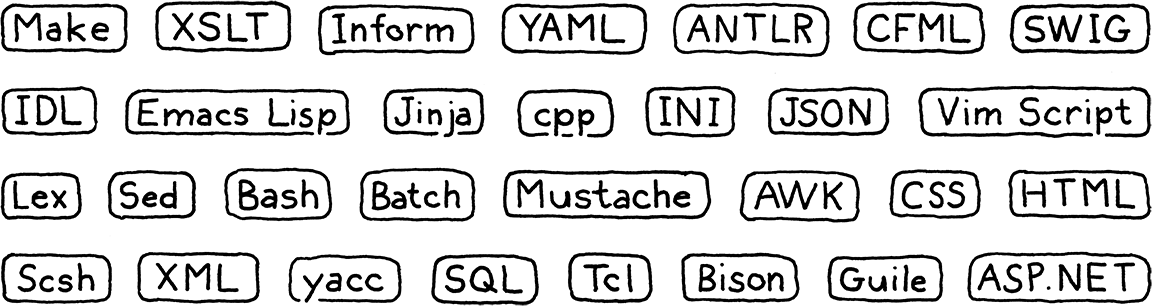
\includegraphics[width=\textwidth]{image/introduction/little-languages.png}
\end{figure}

几乎每个大型软件项目都需要一些这样的工具。如果可以的话,最好重用现有的工具,而不是自己动手实现。一旦考虑到文档、调试器、编辑器支持、语法高亮显示和所有其他可能的障碍,自己实现就成了一项艰巨的任务。

但是,当现有的库不能满足您的需要时,您仍然很有可能发现自己需要一个解析器或其他东西。即使当您重用一些现有的实现时,您也不可避免地需要调试和维护,并在其内部进行探索。

\subsection{自己实现编程语言是一种很好的锻炼}

长跑运动员有时会在脚踝上绑上重物,或者在空气稀薄的高海拔地区进行训练。当他们卸下自己的负担以后,轻便的肢体和富氧的空气带来了新的相对舒适度,使它们可以跑得更快,更远。

实现一门语言是对编程技能的真正考验。代码很复杂,而性能很关键。您必须掌握递归、动态数组、树、图和哈希表。您在日常编程中至少使用过哈希表,但您对它们的理解程度有多高呢?嗯,等我们从头完成我们的作品之后,我相信您会理解的。

虽然我想说明解释器并不像您想的那样令人生畏,但实现一个好的解释器仍然是一个挑战。学会了它,您就会成为一个更强大的程序员,并且在日常工作中也能更加聪明地使用数据结构和算法。

\subsection{一个额外的原因}

这最后一个原因我很难承认,因为它是很私密的理由。自从我小时候学会编程以来,我就觉得语言有种神奇的力量。当我第一次一个键一个键地输入BASIC程序时,我无法想象BASIC语言本身是如何制作出来的。

后来,当我的大学朋友们谈论他们的编译器课程时,脸上那种既敬畏又恐惧的表情足以让我相信,语言黑客是另一种人,某种获得了通向神秘艺术的特权的巫师。

这是一个迷人的形象,但它也有黑暗的一面。我感觉自己不像个巫师,所以我认为自己缺乏加入秘社所需的先天品质。 尽管自从我在学校笔记本上拼写关键词以来,我一直对语言着迷,但我花了数十年的时间鼓起勇气尝试真正地学习它们。那种 “神奇”的品质,那种排他性的感觉,将我挡在门外。

当我最终开始拼凑我自己的小编译器时,我很快意识到,根本就没有魔法。它只是代码,而那些掌握语言的人也只是人。

有一些技巧您在语言之外不会经常遇到,而且有些部分有点难。但不会比您克服的其他障碍更困难。我希望,如果您对语言感到害怕,而这本书能帮助您克服这种恐惧,也许我会让您比以前更勇敢一点。

而且,说不准,你也许会创造出下一个伟大的语言,毕竟总要有人做。

\section{本书的组织方式}

这本书分为三个部分。您现在正在读的是第一部分。这部分用了几章来让您进入状态,教您一些语言黑客使用的行话,并向您介绍我们将要实现的语言Lox。

其他两个部分则分别构建一个完整的Lox解释器。在这些部分中,每个章节的结构都是相同的。 每一章节挑选一个语言功能点,教您背后对应的概念,并逐步介绍实现方法。

我花了不少时间去试错,但我还是成功地把这两个解释器按照章节分成了一些小块,每一小块的内容都会建立在前面几章的基础上,但不需要后续章节的知识。从第一章开始,你就会有一个可以运行和使用的工作程序。随着章节的推移,它的功能越来越丰富,直到你最终拥有一门完整的语言。

除了大量妙趣横生的英文段落,章节中还会包含一些其它的惊喜:

\subsection{代码}

本书是关于制作解释器的,所以其中会包含真正的代码。所需要的每一行代码都需要包含在内,而且每个代码片段都会告知您需要插入到实现代码中的什么位置。

许多其他的语言书籍和语言实现都使用Lex和Yacc这样的工具,也就是所谓的\textbf{编译器——编译器},可以从一些更高层次的(语法)描述中自动生成一些实现的源文件。这些工具有利有弊,而且双方都有强烈的主张——有些人可能将其说成是信仰。

我们这里不会使用这些工具。我想确保魔法和困惑不会藏在黑暗的角落,所以我们会选择手写所有代码。正如您将看到的,这并没有听起来那么糟糕,因为这意味着您将真正理解每一行代码以及两种解释器的工作方式。

一本书和“真实世界”的条件是有区别的,因此这里的代码风格可能并不是可维护生产软件的最佳方式。可能我对某些写法是无所谓的,比如省略\textit{private}或者声明全局变量,请理解我这样做是为了让您更容易看懂代码。书页不像IDE窗口那么宽,所以每一个字符都很珍贵。

另外,代码也不会有太多的注释。这是因为每一部分代码前后,都使用了一些真的很简洁的文字来对其进行解释。当你写一本书来配合你的程序时,欢迎你也省略注释。否则,你可能应该比我使用更多的\textit{//}。

虽然这本书包含了每一行代码,并教授了每一行代码的含义,但它没有描述编译和运行解释器所需的机制。我假设您可以在IDE中选择一个makefile或一个项目导入,以使代码运行。 这类说明很快就会过时,我希望这本书能像XO白兰地一样醇久,而不是像家酿酒(一样易过期)。

\subsection{代码片段}

因为这本书包含了实现所需的每一行代码,所以代码片段相当精确。此外,即使是在缺少主要功能的时候,我也尝试将程序保持在可运行状态。因此我们有时会添加临时代码,这些代码将在以后的代码段中替换。

一个完整的代码片段可能如下所示:

\begin{code}{java}{2-6}{lox/Scanner.java,在scanToken()中替换1行}
default:
  if (isDigit(c)) {
    number();
  } else {
    Lox.error(line, "Unexpected character.");
  }
  break;
\end{code}

中间是要添加的新代码。这部分代码的上面或下面可能有一些淡出的行,以显示它在周围代码中的位置。还会附有一小段介绍,告诉您在哪个文件中以及在哪里放置代码片段。如果简介说要“替换x行”,表明在浅色的行之间有一些现有的代码需要删除,并替换为新的代码片段。

\subsection{题外话}

题外话中包含传记简介、历史背景、对相关主题的引用以及对其他要探索的领域的建议。您无需深入了解就可以理解本书的后续部分,因此可以根据需要跳过它们。我不会批评你,但我可能会有些难过。

\subsection{挑战}

每章结尾都会有一些练习题。不像教科书中的习题集那样用于回顾已讲述的内容,这些习题是为了帮助您学习更多的知识,而不仅仅是本章中的内容。它们会迫使您走出文章指出的路线,自行探索。它们将要求您研究其他语言,弄清楚如何实现功能,换句话说,就是使您走出舒适区。

克服挑战,您将获得更广泛的理解,也可能遇到一些挫折。如果您想留在旅游巴士的舒适区内,也可以跳过它们。都随你便。

\subsection{设计笔记}

大多数编程语言书籍都是严格意义上的编程语言\textit{实现}书籍。他们很少讨论如何\textit{设计}正在实现的语言。实现之所以有趣,是因为它的定义是很精确的。我们程序员似乎很喜欢黑白、1和0这样的事物。

就个人而言,我认为世界只需要这么多的FORTRAN 77实现。在某个时候,您会发现自己正在设计一种新的语言。一旦开始这样做,方程式中较柔和,人性化的一面就变得至关重要。诸如哪些功能易于学习,如何在创新和熟悉度之间取得平衡,哪种语法更易读以及对谁有帮助。

所有这些都会对您的新语言的成功产生深远的影响。我希望您的语言取得成功,因此在某些章节中,我以一篇“设计笔记”结尾,这些是关于编程语言的人文方面的一些文章。我并不是这方面的专家——我不确定是否有人真的精通这些,因此,请您在阅读这些文字的时候仔细评估。这样的话,这些文字就能成为您思考的食材,这也正是我的目标。

\section{第一个解释器}

我们将用Java编写第一个解释器jlox。(这里的)主要关注点是概念。我们将编写最简单,最干净的代码,以正确实现该语言的语义。这样能够帮助我们熟悉基本技术,并磨练对语言表现形式的确切理解。

Java是一门很适合这种场景的语言。它的级别足够高,我们不会被繁琐的实现细节淹没,但代码仍是非常明确的。与脚本语言不同的是,它的底层没有隐藏太过复杂的机制,你可以使用静态类型来查看正在处理的数据结构。

我选择Java还有特别的原因,就是因为它是一种面向对象的语言。这种范式在90年代席卷了整个编程世界,如今已成为数百万程序员的主流思维方式。很有可能您已经习惯了将代码组织到类和方法中,因此我们将让您在舒适的环境中学习。

虽然学术语言专家有时瞧不起面向对象语言,但事实上,它们即使在语言工作中也被广泛使用。GCC和LLVM是用C++编写的,大多数JavaScript虚拟机也是这样。面向对象的语言无处不在,并且针对该语言的工具和编译器通常是用同一种语言编写的。

最后,Java非常流行。这意味着您很有可能已经了解它了,所以你要学习的东西就更少了。如果您不太熟悉Java,也请不要担心。我尽量只使用它的最小子集。我使用Java 7中的菱形运算符使代码看起来更简洁,但就“高级”功能而言,仅此而已。如果您了解其它面向对象的语言(例如C\#或C++),就没有问题。

在第二部分结束时,我们将得到一个简单易读的实现。但是我们得到的不会是一个快速的解释器。它还是利用了Java虚拟机自身的运行时工具。我们想要学习Java本身是如何实现这些东西的。

\section{第二个解释器}

所以在下一部分,我们将从头开始,但这一次是用C语言。C语言是理解实现编译器工作方式的完美语言,一直到内存中的字节和流经CPU的代码。

我们使用C语言的一个重要原因是,我可以向您展示C语言特别擅长的东西,但这并不意味着您需要非常熟练地使用它。您不必是丹尼斯·里奇(Dennis Ritchie)的转世,但也不应被指针吓倒。

如果你(对C的掌握)还没到那一步,找一本关于C的入门书,仔细阅读,读完后再回来。作为回报,从这本书中你将成为一个更优秀的C程序员。可以想想有多少语言实现是用C完成的: Lua、CPython和Ruby的MRI等,这里仅举几例。

在我们的C解释器clox中,我们不得不自己实现那些Java免费提供给我们的东西。我们将编写自己的动态数组和哈希表。我们将决定对象在内存中的表示方式,并构建一个垃圾回收器来回收它。

我们的Java版实现专注于正确性。既然我们已经完成了,那么我们就要变得越来越快。我们的C解释器将包含一个编译器,该编译器会将Lox转换为有效的字节码形式(不用担心,我很快就会讲解这是什么意思)之后它会执行对应的字节码。这与Lua,Python,Ruby,PHP和许多其它成功语言的实现所使用的技术相同。

我们甚至会尝试进行基准测试和优化。到最后,我们将为lox语言提供一个强大,准确,快速的解释器,并能够不落后于其他专业水平的实现。对于一本书和几千行代码来说已经不错了。

\section{挑战}

\begin{enumerate}
  \item 在我编写的这个小系统中,至少有六种特定领域语言(DSL),它们是什么?
  \item 使用Java编写并运行一个“Hello, world!”程序,设置你需要的makefile或IDE项目使其正常工作。如果您有调试器,请先熟悉一下,并在程序运行时对代码逐步调试。
  \item 对C也进行同样的操作。为了练习使用指针,可以定义一个堆分配字符串的双向链表。编写函数以插入,查找和删除其中的项目。 测试编写的函数。
\end{enumerate}

\section{设计笔记:名字是什么?}

写这本书最困难的挑战之一是为它所实现的语言取个名字。我翻了好几页的备选名才找到一个合适的。当你某一天开始构建自己的语言时,你就会发现命名是非常困难的。一个好名字要满足几个标准:

\begin{enumerate}
  \item \textbf{尚未使用}。如果您不小心使用了别人的名字,就可能会遇到各种法律和社会上的麻烦。
  \item \textbf{容易发音}。如果一切顺利,将会有很多人会说和写您的语言名称。 超过几个音节或几个字母的任何内容都会使他们陷入无休止的烦恼。
  \item \textbf{足够独特,易于搜索}。人们会Google你的语言的名字来了解它,所以你需要一个足够独特的单词,以便大多数搜索结果都会指向你的文档。不过,随着人工智能搜索引擎数量的增加,这已经不是什么大问题了。但是,如果您将语言命名为“for”,那对用户基本不会有任何帮助。
  \item \textbf{在多种文化中,都没有负面的含义}。这很难防范,但是值得深思。Nimrod的设计师最终将其语言重命名为“Nim”,因为太多的人只记得Bugs Bunny使用“Nimrod”作为一种侮辱(其实是讽刺)。
\end{enumerate}

如果你潜在的名字通过了考验,就保留它吧。不要纠结于寻找一个能够抓住你语言精髓的名称。如果说世界上其他成功的语言的名字教会了我们什么的话,那就是名字并不重要。您所需要的只是一个相当独特的标记。

\chapter{全书地图}

\epigraph{你必须要有一张地图,无论它是多么粗糙。否则你就会到处乱逛。在《指环王》中,我从未让任何人在某一天走得超出他力所能及的范围。}{托尔金}

我们不想到处乱逛,所以在我们开始之前,让我们先浏览一下以前的语言实现者所绘制的领土。它能帮助我们了解我们的目的地和其他人采用的备选路线。

首先,我先做个简单说明。本书的大部分内容都是关于语言的\textit{实现},它与\textit{语言本身}这种柏拉图式的理想形式有所不同。诸如“堆栈”,“字节码”和“递归下降”之类的东西是某个特定实现中可能使用的基本要素。从用户的角度来说,只要最终产生的装置能够忠实地遵循语言规范,它内部的都是实现细节。

我们将会花很多时间在这些细节上,所以如果我每次提及的时候都写“语言实现”,我的手指都会被磨掉。相反,除非有重要的区别,否则我将使用“语言”来指代一种语言或该语言的一种实现,或两者皆有。

\section{语言的各部分}

自计算机的黑暗时代以来,工程师们就一直在构建编程语言。当我们可以和计算机对话的时候,我们发现这样做太难了,于是我们寻求电脑的帮助。我觉得很有趣的是,即使今天的机器确实快了一百万倍,存储空间也大了几个数量级,但我们构建编程语言的方式几乎没有改变。

尽管语言设计师所探索的领域辽阔,但他们所走过的路却很少。并非每种语言都采用完全相同的路径(有些采用一种或两种捷径),但除此之外,从海军少将Grace Hopper的第一个COBOL编译器,一直到一些热门的新移植到JavaScript的语言,它们的“文档”完全是由Git仓库中一个编辑得很差的README组成的。

我把一个语言实现可能选择的路径网络类比为爬山。你从最底层开始,程序是原始的源文本,实际上只是一串字符。每个阶段都会对程序进行分析,并将其转换为更高层次的表现形式,从而使语义(作者希望计算机做什么)变得更加明显。

最终我们达到了峰顶。我们可以鸟瞰用户的程序,可以看到他们的代码含义是什么。我们开始从山的另一边下山。我们将这个最高级的表示形式转化为连续的较低级别的形式,从而越来越接近我们所知道的如何让CPU真正执行的形式。

\begin{figure}[htbp]
  \centering
  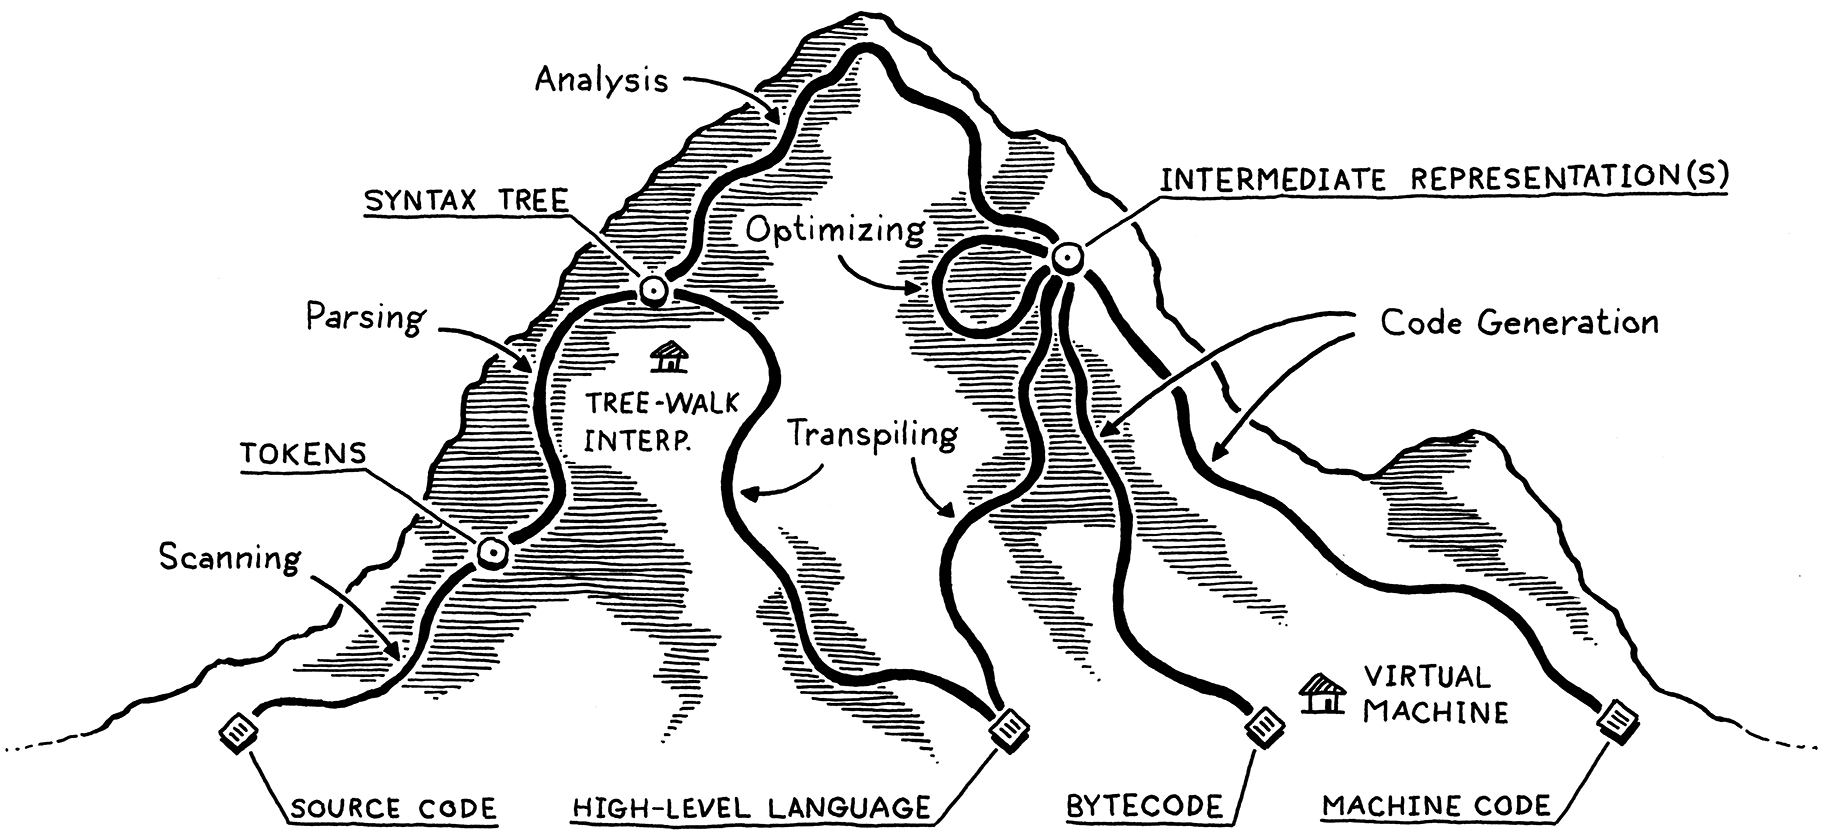
\includegraphics[width=\textwidth]{image/a-map-of-the-territory/mountain.png}
\end{figure}

让我们沿着每一条路线和每一个感兴趣的地方走一遍。我们的旅程从左边的用户源代码的纯文本开始。

\begin{figure}[htbp]
  \centering
  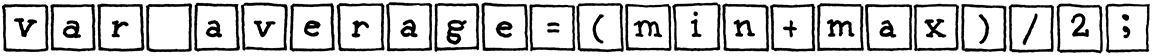
\includegraphics[width=\textwidth]{image/a-map-of-the-territory/string.png}
\end{figure}

\subsection{扫描}

第一步是\textbf{扫描},也就是所谓的\textbf{词法},或者说(如果你想给别人留下深刻印象)\textbf{词法分析}。它们的意思都差不多。我喜欢“lexing”,因为这听起来像是一个邪恶的超级大坏蛋会做的事情,但我还是用“scanning”,因为它似乎更常见一些。

扫描器(或词法解析器)接收线性字符流,并将它们组合成一系列更类似于“单词”的东西。在编程语言中,这些词的每一个都被称为\textbf{标记}。有些标记是单个字符,比如(和,。其他的可能是几个字符长的,比如数字(123)、字符串字元("hi!")和标识符(min)。

源文件中的一些字符实际上没有任何意义。空格通常是无关紧要的,而注释,从定义就能看出来,会被语言忽略。扫描仪通常会丢弃这些字符,留下一个干净的有意义的标记序列。

\begin{figure}[htbp]
  \centering
  
\includegraphics[width=\textwidth]{image/a-map-of-the-territory/tokens.png}
\end{figure}

\subsection{语法分析}

下一步是\textbf{解析}。这就是我们从句法中得到\textbf{语法}的地方——语法能够将较小的部分组成较大的表达式和语句。你在英语课上画过句子图吗?如果有,你就做了解析器所做的事情,区别在于,英语中有成千上万的“关键字”和大量的歧义,而编程语言要简单得多。

\textbf{解析器}接受标记的平面序列,并构建反映语法嵌套本质的树结构。这些树有两个不同的名称:\textbf{解析树}或\textbf{抽象语法树},这取决于它们与源语言的语法结构有多接近。在实践中,语言黑客通常称它们为“\textbf{语法树}”、“\textbf{AST}”,或者干脆直接说“\textbf{树}”。

\begin{figure}[htbp]
  \centering
  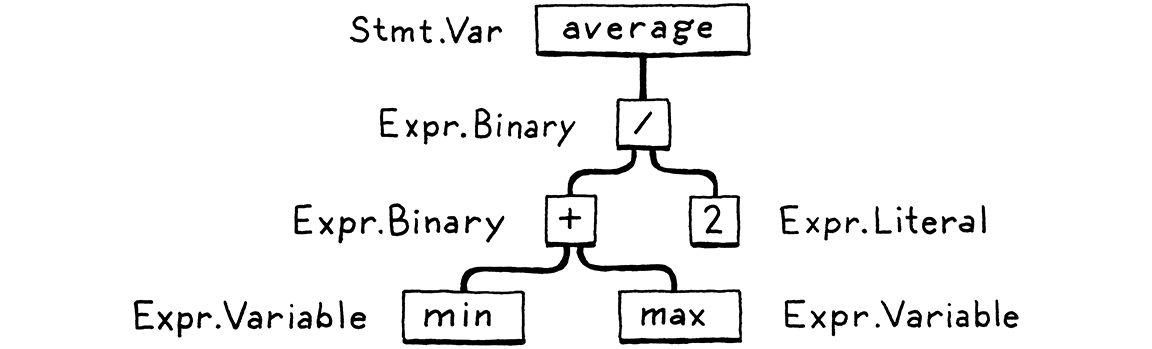
\includegraphics[width=\textwidth]{image/a-map-of-the-territory/ast.png}
\end{figure}

解析在计算机科学中有着悠久而丰富的历史,它与人工智能界有着密切的联系。今天用于解析编程语言的许多技术最初是由人工智能研究人员设想的,他们试图让计算机与我们对话,以解析人类语言。

事实证明,相对那些解析器能够处理的严格语法来说,人类语言太混乱了;但对于编程语言中更简单的人工语法来说,人类语言却是完美的。唉,可惜我们这些有缺陷的人类仍然会错误地使用这些简单的语法,因此解析器的工作还包括通过报告\textbf{语法错误}让我们知道出错了。

\subsection{静态分析}

在所有实现中,前两个阶段都非常相似。现在,每种语言的个性化特征开始发挥作用。至此,我们知道了代码的语法结构(诸如哪些表达式嵌套在其他表达式中)之类的东西,但是我们知道的也就仅限于此了。

在a+b这样的表达式中,我们知道我们要把a和b相加,但我们不知道这些名字指的是什么。它们是局部变量吗?全局变量?它们在哪里被定义?

大多数语言所做的第一点分析叫做\textbf{绑定}或\textbf{解析}。对于每一个\textbf{标识符},我们都要找出定义该名称的地方,并将两者连接起来。这就是\textbf{作用域}的作用—在这个源代码区域中,某个名字可以用来引用某个声明。

如果语言是静态类型的,这时我们就进行类型检查。一旦我们知道了a和b的声明位置,我们也可以弄清楚它们的类型。然后如果这些类型不支持互相累加,我们就会报告一个\textbf{类型错误}。

深吸一口气。我们已经到达了山顶,并对用户的程序有了全面的了解。所有这些从分析中可见的语义信息都需要存储在某个地方。我们可以把它藏在几个地方:

\begin{itemize}
  \item 通常,它会被直接存储在语法树本身的\textbf{属性}中—属性是节点中的额外字段,这些字段在解析时不会初始化,但在稍后会进行填充。
  \item 有时,我们可能会将数据存储在外部的查找表中。通常,该表的关键字是标识符,即变量和声明的名称。在这种情况下,我们称其为\textbf{符号表},并且其中与每个键关联的值告诉我们该标识符所指的是什么。
  \item 最强大的记录工具是将树转化为一个全新的数据结构,更直接地表达代码的语义。这是下一节的内容。
\end{itemize}

到目前为止,所有内容都被视为实现的\textbf{前端}。您可能会猜至此以后是\textbf{后端},其实并不是。在过去的年代,当“前端”和“后端”被创造出来时,编译器要简单得多。后来,研究人员在两个半部之间引入了新阶段。威廉·沃尔夫(William Wulf)和他的同伴没有放弃旧术语,而是新添加了一个迷人但有点自相矛盾的名称“\textbf{中端}”。

\subsection{中间表示}

你可以把编译器看成是一条流水线,每个阶段的工作是把代表用户代码的数据组织起来,使下一阶段的实现更加简单。管道的前端是针对程序所使用的源语言编写的。后端关注的是程序运行的最终架构。

在中间阶段,代码可能被存储在一些\textbf{中间表示}(\textbf{intermediate representation}, 也叫\textbf{IR})中,这些中间表示与源文件或目标文件形式都没有紧密的联系(因此叫作“中间”)。相反,IR充当了这两种语言之间的接口。

这可以让你更轻松地支持多种源语言和目标平台。假设你想实现Pascal、C和Fortran编译器,并且你的目标平台的体系结构是:x86、ARM,还有SPARC。通常情况下,这意味着你需要写九个完整的编译器:Pascal $\rightarrow$ x86,C $\rightarrow$ ARM,以及其他各种组合。

一个共享的中间表示可以大大减少这种情况。你为每个产生IR的源语言写\textit{一个}前端。然后为每个目标平台写\textit{一个}后端。现在,你可以将这些混搭起来,得到每一种组合。

还有一个重要的原因是,我们可能希望将代码转化为某种形式,使语义更加明确...。

\subsection{优化}

一旦我们理解了用户程序的含义,我们就可以自由地用另一个具有相同语义但实现效率更高的程序来交换它—我们可以对它进行\textbf{优化}。

一个简单的例子是\textbf{常量折叠}:如果某个表达式求值得到的始终是完全相同的值,我们可以在编译时进行求值,并用其结果替换该表达式的代码。如果用户输入:

\begin{code}{java}{}{}
pennyArea = 3.14159 * (0.75 / 2) * (0.75 / 2);
\end{code}

我们可以在编译器中完成所有的算术运算,并将代码更改为:

\begin{code}{java}{}{}
pennyArea = 0.4417860938;
\end{code}

优化是编程语言业务的重要组成部分。许多语言黑客把他们的整个职业生涯都花在了这里,竭尽所能地从他们的编译器中挤出每一点性能,以使他们的基准测试速度提高一个百分点。这可能会成为一种困扰。

我们通常会跳过本书中的棘手问题。许多成功的语言令人惊讶地很少进行编译期优化。例如,Lua和CPython生成相对未优化的代码,并将其大部分性能优化工作集中在运行时上。

\subsection{代码生成}

我们已经将所有可以想到的优化应用到了用户程序中。最后一步是将其转换为机器可以实际运行的形式。换句话说,\textbf{生成代码}(或\textbf{代码生成}),这里的“代码”通常是指CPU运行的类似于汇编的原始指令,而不是人类可能想要阅读的“源代码”。

最后,我们到了\textbf{后端},从山的另一侧开始向下。从现在开始,随着我们越来越接近于思维简单的机器可以理解的东西,我们对代码的表示变得越来越原始,就像逆向进化。

我们需要做一个决定。我们是为真实CPU还是虚拟CPU生成指令? 如果我们生成真实的机器代码,则会得到一个可执行文件,操作系统可以将其直接加载到芯片上。原生代码快如闪电,但生成它需要大量工作。当今的体系结构包含大量指令,复杂的流水线和足够塞满一架747行李舱的历史包袱。

使用芯片的语言也意味着你的编译器是与特定的架构相绑定的。如果你的编译器以x86机器代码为目标,那么它就无法在ARM设备上运行。一直到60年代,在计算机体系结构的寒武纪大爆发期间,这种缺乏可移植性的情况是一个真正的障碍。

为了解决这个问题,像BCPL的Martin Richards和Pascal的Niklaus Wirth这样的黑客,让他们的编译器生成虚拟机代码。他们不是为真正的芯片编写指令,而是为一个假设的、理想化的机器编写代码。Wirth称这种\textbf{p-code}为“可移植代码”,但今天,我们通常称它为\textbf{字节码},因为每条指令通常都是一个字节长。

这些合成指令的设计是为了更紧密地映射到语言的语义上,而不必与任何一个计算机体系结构的特性和它积累的历史错误绑定在一起。你可以把它想象成语言底层操作的密集二进制编码。

\subsection{虚拟机}

如果你的编译器产生了字节码,你的工作还没有结束。因为没有芯片可以解析这些字节码,因此你还需要进行翻译。同样,您有两个选择。您可以为每个目标体系结构编写一个小型编译器,将字节码转换为该机器的本机代码。您仍然需要针对您支持的每个芯片做一些工作,但最后这个阶段非常简单,你可以在你支持的所有机器上重复使用编译器管道的其余部分。你基本上是把你的字节码作为一个中介码。

或者,您可以编写\textbf{虚拟机(VM)},该程序可在运行时模拟支持虚拟架构的虚拟芯片。在虚拟机中运行字节码比提前将其翻译成本地代码要慢,因为每条指令每次执行时都必须在运行时模拟。作为回报,你得到的是简单性和可移植性。用比如说C语言实现你的虚拟机,你就可以在任何有C编译器的平台上运行你的语言。这就是我们在本书中构建的第二个解释器的工作原理。

\subsection{运行时}

我们终于将用户程序锤炼成可以执行的形式。最后一步是运行它。如果我们将其编译为机器码,我们只需告诉操作系统加载可执行文件,然后就可以运行了。如果我们将它编译成字节码,我们需要启动VM并将程序加载到其中。

在这两种情况下,除了最基本的底层语言外,我们通常需要我们的语言在程序运行时提供一些服务。例如,如果语言自动管理内存,我们需要一个垃圾收集器去回收未使用的比特位。如果我们的语言支持instance of测试,这样你就可以看到你有什么类型的对象,那么我们就需要一些表示方法来跟踪执行过程中每个对象的类型。

所有这些东西都是在运行时进行的,所以它被恰当地称为,\textbf{运行时}。在一个完全编译的语言中,实现运行时的代码会直接插入到生成的可执行文件中。比如说,在Go中,每个编译后的应用程序都有自己的一份Go的运行时副本直接嵌入其中。如果语言是在解释器或虚拟机内运行,那么运行时将驻留于虚拟机中。这也就是Java、Python和JavaScript等大多数语言实现的工作方式。

\section{捷径和备选路线}

这是一条漫长的道路,涵盖了你要实现的每个可能的阶段。许多语言的确走完了整条路线,但也有一些捷径和备选路径。

\subsection{单遍编译器}

一些简单的编译器将解析、分析和代码生成交织在一起,这样它们就可以直接在解析器中生成输出代码,而无需分配任何语法树或其他IR。这些\textbf{单遍编译器}限制了语言的设计。您没有中间数据结构来存储程序的全局信息,也不会重新访问任何之前解析过的代码部分。这意味着,一旦您看到某个表达式,就需要足够的知识来正确地对其进行编译。

Pascal和C语言就是围绕这个限制而设计的。在当时,内存非常珍贵,一个编译器可能连整个源文件都无法存放在内存中,更不用说整个程序了。这也是为什么Pascal的语法要求类型声明要先出现在一个块中。这也是为什么在C语言中,你不能在定义函数的代码上面调用函数,除非你有一个明确的前向声明,告诉编译器它需要知道什么,以便生成调用后面函数的代码。

\subsection{树遍历解释器}

有些编程语言在将代码解析为AST后就开始执行代码(可能应用了一点静态分析)。为了运行程序,解释器每次都会遍历语法树的一个分支和叶子,并在运行过程中计算每个节点。

这种实现风格在学生项目和小型语言中很常见,但在通用语言中并不广泛使用,因为它往往很慢。有些人使用“解释器”仅指这类实现,但其他人对“解释器”一词的定义更宽泛,因此我将使用没有歧义的“\textbf{树遍历解释器}”来指代这些实现。我们的第一个解释器就是这样工作的。

\subsection{转译器}

为一种语言编写一个完整的后端可能需要大量的工作。如果您有一些现有的通用IR作为目标,则可以将前端转换到该IR上。否则,您可能会陷入困境。但是,如果您将某些其他\textit{源语言}视为中间表示,该怎么办?

您需要为您的语言编写一个前端。然后,在后端,您可以生成一份与您的语言级别差不多的其他语言的有效源代码字符串,而不是将所有代码\textit{降低}到某个原始目标语言的语义。然后,您可以使用该语言现有的编译工具作为逃离大山的路径,得到某些可执行的内容。

人们过去称之为\textbf{源到源编译器}或\textbf{转换编译器}。随着那些为了在浏览器中运行而编译成JavaScript的各类语言的兴起,它们有了一个时髦的名字—\textbf{转译器}。

虽然第一个编译器是将一种汇编语言翻译成另一种汇编语言,但现今,大多数编译器都适用于高级语言。在UNIX病毒式地传播到各种各样的机器之后,开始了一个悠久的编译器传统,即编译器以C作为输出语言。只要UNIX存在,就可以使用C编译器,并生成有效的代码,因此,以C为目标是让语言在许多体系结构上运行的好方法。

Web浏览器是今天的“机器”,它们的“机器代码”是JavaScript,所以现在似乎几乎所有的语言都有一个以JS为目标的编译器,因为这是让你的代码在浏览器中运行的主要方式。

编译器的前端(扫描器和解析器)看起来跟其他编译器相似。然后,如果源语言只是在目标语言之上包装的简单语法外壳,则它可能会完全跳过分析,并直接输出目标语言中的类似语法。

如果两种语言的语义差异较大,那么你就会看到完整编译器的更多典型阶段,包括分析甚至优化。然后,在代码生成阶段,无需输出一些像机器代码一样的二进制语言,而是在目标语言中生成一串语法正确的源码(好吧,目标代码)。

不管是哪种方式,你再通过目标语言已有的编译管道运行生成的代码,就可以了。

\subsection{即时编译}

最后一个与其说是捷径,不如说是危险的高山争霸赛,最好留给专家。执行代码最快的方法是将代码编译成机器代码,但你可能不知道你的最终用户的机器支持什么架构。该怎么做呢?

您可以做和HotSpot JVM、Microsoft的CLR和大多数JavaScript解释器相同的事情。在终端用户的机器上,当程序加载时(无论是从JS中还是从源代码加载,或者是JVM和CLR的平台无关的字节码),都可以将其编译为对应的本地代码,以适应本机支持的体系结构。自然地,这被称为\textbf{即时编译}。大多数黑客只是说“JIT”,其发音与“fit”押韵。

最复杂的JIT将性能分析钩子插入到生成的代码中,以查看哪些区域对性能最为关键,以及哪些类型的数据正在流经其中。然后,随着时间的推移,它们将通过更高级的优化功能自动重新编译那些热点部分。

\section{编译器和解释器}

现在我已经向你的脑袋里塞满了一大堆编程语言术语,我们终于可以解决一个自远古以来一直困扰着程序员的问题:编译器和解释器之间有什么区别?

事实证明,这就像问水果和蔬菜的区别一样。这看上去似乎是一个非此即彼的选择,但实际上“水果”是一个植物学术语,“蔬菜”是烹饪学术语。严格来说,一个并不意味着对另一个的否定。有不是蔬菜的水果(苹果),也有不是水果的蔬菜(胡萝卜),也有既是水果又是蔬菜的可食用植物,比如西红柿。

\begin{figure}[htbp]
  \centering
  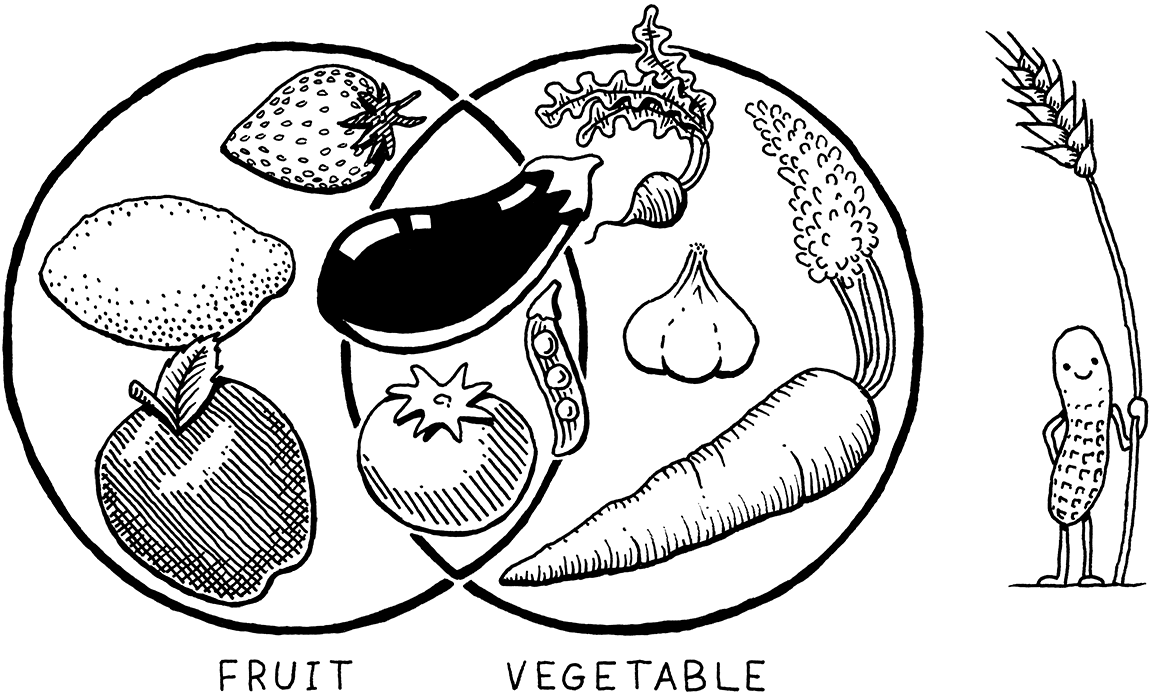
\includegraphics[width=\textwidth]{image/a-map-of-the-territory/plants.png}
\end{figure}

好,回到语言上:

\begin{itemize}
  \item \textbf{编译}是一种实现技术,其中涉及到将源语言翻译成其他语言——通常是较低级的形式。当你生成字节码或机器代码时,你就是在编译。当你移植到另一种高级语言时,你也在编译。
  \item 当我们说语言实现“是\textbf{编译器}”时,是指它会将源代码转换为其他形式,但不会执行。用户必须获取结果输出并自己运行。
  \item 相反,当我们说一个实现“是一个\textbf{解释器}”时,是指它接受源代码并立即执行它。它“从源代码”运行程序。
\end{itemize}

像苹果和橘子一样,某些实现显然是编译器,而不是解释器。GCC和Clang接受您的C代码并将其编译为机器代码。最终用户直接运行该可执行文件,甚至可能永远都不知道使用了哪个工具来编译它。所以这些是C的\textit{编译器}。

在Matz的旧版本的Ruby规范实现中,用户从源代码中运行Ruby。该实现通过遍历语法树对其进行解析并直接执行。期间都没有发生其他的转换,无论是在实现内部还是以任何用户可见的形式。所以这绝对是一个Ruby的\textit{解释器}。

但是CPython呢?当你使用它运行你的Python程序时,代码会被解析并转换为内部字节码格式,然后在虚拟机内部执行。从用户的角度来看,这显然是一个解释器——他们是从源代码开始运行自己的程序。但如果你看一下CPython的内部,你会发现肯定有一些编译工作在进行。

答案是两者兼而有之。CPython是一个解释器,但他也\textit{有}一个编译器。实际上,大多数脚本语言都以这种方式工作,如您所见:

\begin{figure}[htbp]
  \centering
  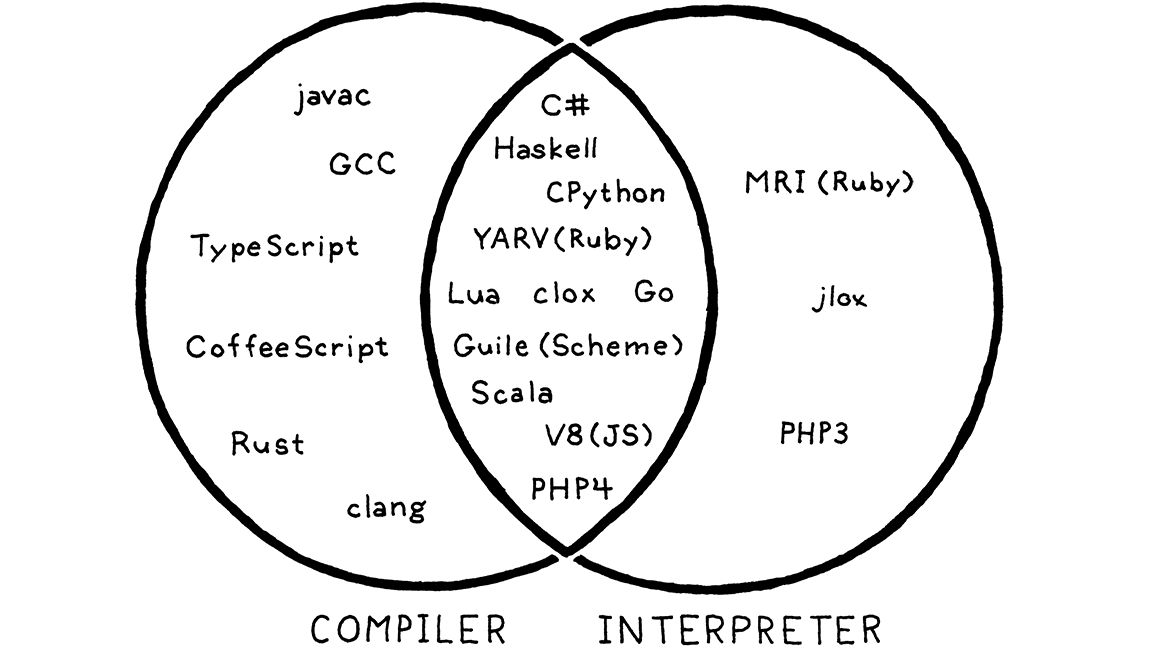
\includegraphics[width=\textwidth]{image/a-map-of-the-territory/venn.png}
\end{figure}

中间那个重叠的区域也是我们第二个解释器所在的位置,因为它会在内部编译成字节码。所以,虽然本书名义上是关于解释器的,但我们也会涉及一些编译的内容。

\section{我们的旅程}

一下子有太多东西要消化掉。别担心。这一章并不是要求你理解所有这些零碎的内容。我只是想让你们知道它们是存在的,以及大致了解它们是如何组合在一起的。

当您探索本书本书所指导的路径之外的领域时,这张地图应该对你很有用。我希望你自己出击,在那座山里到处游走。

但是,现在,是我们自己的旅程开始的时候了。系好你的鞋带,背好你的包,走吧。从这里开始,你需要关注的是你面前的路。

\section{挑战}

\begin{enumerate}
  \item 选择一个你喜欢的语言的开源实现。下载源代码,并在其中探索。试着找到实现扫描器和解析器的代码,它们是手写的,还是用Lex和Yacc等工具生成的?(存在.l或.y文件通常意味着后者)
  \item 实时编译往往是实现动态类型语言最快的方法,但并不是所有的语言都使用它。有什么理由不采用JIT呢?
  \item 大多数可编译为C的Lisp实现也包含一个解释器,该解释器还使它们能够即时执行Lisp代码。为什么?
\end{enumerate}

\chapter{Lox编程语言}

\epigraph{你能够为别人做什么比做早餐更好的事情吗?}{布尔丹}

我们将用本书的其余部分来照亮Lox语言的每一个黑暗和杂乱的角落,但如果让你在对目标一无所知的情况下,就立即开始为解释器编写代码,这似乎很残忍。

与此同时,我也不想在您编码之前,就把您拖入大量的语言和规范术语中。所以这是一个温和、友好的Lox介绍,它会省去很多细节和边缘情况。后面我们有足够的时间来解决这些问题。

\section{Hello, Lox}

下面是你对Lox的第一次体验:

\begin{code}{js}{}{}
// Your first Lox program!
print "Hello, world!";
\end{code}

正如那句//行注释和后面的分号所暗示的那样,Lox的语法是C语言家族的成员之一。(因为print是一个内置语句,而不是库函数,所以字符串周围没有括号。)

这里,我并不是想说C语言具有出色的语法。如果我们想要一些优雅的东西,我们可能会模仿Pascal或Smalltalk。如果我们想要完全体现斯堪的纳维亚家具的极简主义风格,我们会实现一个Scheme。这些都有其优点。

但是,类C的语法所具有的反而是一些在语言中更有价值的东西:\textit{熟悉度}。我知道你已经对这种风格很熟悉了,因为我们将用来实现Lox的两种语言——Java和C——也继承了这种风格。让Lox使用类似的语法,你就少了一件需要学习的事情。

\section{高级语言}

虽然这本书最终比我所希望的要大,但它仍然不够大,无法将Java这样一门庞大的语言放进去。为了在有限的篇幅里容纳两个完整的Lox实现,Lox本身必须相当紧凑。

当我想到那些小而有用的语言时,我脑海中浮现的是像JavaScript、Scheme和Lua这样的高级“脚本”语言。在这三种语言中,Lox看起来最像JavaScript,主要是因为大多数C语法语言都是这样的。稍后我们将了解到,Lox实现作用域的方式与Scheme密切相关。我们将在第三部分中构建的C风格的Lox很大程度上得益于Lua的干净、高效的实现。

Lox与这三种语言有两个共同之处:

\subsection{动态类型}

Lox是动态类型的。变量可以存储任何类型的值,单个变量甚至可以在不同时间存储不同类型的值。如果尝试对错误类型的值执行操作(例如,将数字除以字符串),则会在运行时检测到错误并报告。

喜欢静态类型的原因有很多,但它们都比不上为Lox选择动态类型的实际原因。静态类型系统需要学习和实现大量的工作。跳过它会让你的语言更简单,也可以让本书更短。如果我们将类型检查推迟到运行时,我们将可以更快地启动解释器并执行代码。

\subsection{自动内存管理}

高级语言的存在是为了消除容易出错的低级工作,还有什么比手动管理存储的分配和释放更繁琐的呢?没有人会抬起头来迎接早晨的阳光,“我迫不及待想找到正确的位置,调用free()方法来准备今天每个字节需要分配的内存!”

有两种主要的内存管理技术:\textbf{引用计数}和\textbf{跟踪垃圾收集}(通常仅称为“\textbf{垃圾收集}”或“\textbf{GC}”)。引用计数器的实现要简单得多——我想这就是为什么Perl、PHP和Python一开始都使用该方式的原因。但是,随着时间的流逝,引用计数的限制变得太麻烦了。所有这些语言最终都添加了完整的跟踪GC或至少一种足以清除对象循环的管理方式。

追踪垃圾收集有一个可怕的名声。在原始内存的层面上工作是有点折磨人的。调试GC有时会让你在梦中看到hex dumps。但是,请记住,这本书是关于驱散魔法和杀死那些怪物的,所以我们要写出自己的垃圾收集器。我想你会发现这个算法相当简单,而且实现起来很有趣。

\section{数据类型}

在Lox的小宇宙中,构成所有物质的原子是内置的数据类型。只有几个:

\textbf{Booleans}——没有逻辑就不能编码,没有布尔值也就没有逻辑。“真”和“假”,就是软件的阴与阳。与某些古老的语言重新利用已有类型来表示真假不同,Lox具有专用的布尔类型。在这次探险中,我们可能会有些粗暴,但我们不是野蛮人。

显然,有两个布尔值,每个值都有一个字面量:

\begin{code}{js}{}{}
true;  // Not false.
false; // Not *not* false.
\end{code}

\textbf{Numbers}——Lox只有一种数字:双精度浮点数。由于浮点数还可以表示各种各样的整数,因此可以覆盖很多领域,同时保持简单。

功能齐全的语言具有多种数字语法——十六进制,科学计数法,八进制和各种有趣的东西。我们只使用基本的整数和十进制文字:

\begin{code}{js}{}{}
1234;  // An integer.
12.34; // A decimal number.
\end{code}

\textbf{Strings}——在第一个示例中,我们已经看到一个字符串字面量。与大多数语言一样,它们用双引号引起来:

\begin{code}{js}{}{}
"I am a string";
"";    // The empty string.
"123"; // This is a string, not a number.
\end{code}

我们在实现它们时会看到,在这个无害的字符序列中隐藏了相当多的复杂性。

\textbf{Nil}——还有最后一个内置数据,它从未被邀请参加聚会,但似乎总是会出现。它代表“没有价值”。在许多其他语言中称为“null”。在Lox中,我们将其拼写为nil。(当我们实现它时,这将有助于区分Lox的nil与Java或C的null)

有一些很好的理由表明在语言中不使用空值是合理的,因为空指针错误是我们行业的祸害。如果我们使用的是静态类型语言,那么禁止它是值得的。然而,在动态类型中,消除它往往比保留它更加麻烦。

\section{表达式}

如果内置数据类型及其字面量是原子,那么表达式必须是分子。其中大部分大家都很熟悉。

\subsection{算术运算}

Lox具备了您从C和其他语言中了解到的基本算术运算符:

\begin{code}{js}{}{}
add + me;
subtract - me;
multiply * me;
divide / me;
\end{code}

操作符两边的子表达式都是\textbf{操作数}。因为有两个操作数,它们被称为\textbf{二元}运算符(这与二进制的1和0二元没有关联)。由于操作符固定在操作数的中间,因此也称为\textbf{中缀}操作符,相对的,还有\textbf{前缀}操作符(操作符在操作数前面)和\textbf{后缀}操作符(操作符在操作数后面)。

有一个数学运算符既是中缀运算符也是前缀运算符,-运算符可以对数字取负:

\begin{code}{js}{}{}
-negateMe;
\end{code}

所有这些操作符都是针对数字的,将任何其他类型操作数传递给它们都是错误的。唯一的例外是+运算符——你也可以传给它两个字符串将它们串接起来。

\subsection{比较与相等}

接下来,我们有几个返回布尔值的操作符。我们可以使用旧的比较操作符来比较数字(并且只能比较数字):

\begin{code}{js}{}{}
less < than;
lessThan <= orEqual;
greater > than;
greaterThan >= orEqual;
\end{code}

我们可以测试两个任意类型的值是否相等:

\begin{code}{js}{}{}
1 == 2;         // false.
"cat" != "dog"; // true.
\end{code}

即使是不同类型也可以:

\begin{code}{js}{}{}
314 == "pi"; // false.
\end{code}

不同类型的值\textit{永远不会}相等:

\begin{code}{js}{}{}
123 == "123"; // false.
\end{code}

我通常是反对隐式转换的。

\subsection{逻辑运算}

取非操作符,是前缀操作符!,如果操作数是true,则返回false,反之亦然:

\begin{code}{js}{}{}
!true;  // false.
!false; // true.
\end{code}

其他两个逻辑操作符实际上是表达式伪装下的控制流结构。and表达式用于确认两个操作数是否\textit{都是}true。如果左侧操作数是false,则返回左侧操作数,否则返回右侧操作数:

\begin{code}{js}{}{}
true and false; // false.
true and true;  // true.
\end{code}

or表达式用于确认两个操作数中任意一个(或者都是)为true。如果左侧操作数为true,则返回左侧操作数,否则返回右侧操作数:

\begin{code}{js}{}{}
false or false; // false.
true or false;  // true.
\end{code}

and和or之所以像控制流结构,是因为它们会\textbf{短路}。如果左操作数为假,and不仅会返回左操作数,在这种情况下,它甚至不会计算右操作数。反过来,(“相对的”?)如果or的左操作数为真,右操作数就会被跳过。

\subsection{优先级与分组}

所有这些操作符都具有与c语言相同的优先级和结合性(当我们开始解析时,会进行更详细的说明)。在优先级不满足要求的情况下,你可以使用()来分组:

\begin{code}{js}{}{}
var average = (min + max) / 2;
\end{code}

我把其他典型的操作符从我们的小语言中去掉了,因为它们在技术上不是很有趣。没有位运算、移位、取模或条件运算符。我不是在给你打分,但如果你通过自己的方式来完成支持这些运算的Lox实现,你会在我心中得到额外的加分。

这些都是表达式形式(除了一些与我们将在后面介绍的特定特性相关的),所以让我们继续。

\section{语句}

现在我们来看语句。表达式的主要作用是产生一个\textit{值},语句的主要作用是产生一个\textit{作用}。由于根据定义,语句不求值,因此必须以某种方式改变世界(通常是修改某些状态,读取输入或产生输出)才能有用。

您已经看到了几种语句。 第一个是:

\begin{code}{js}{}{}
print "Hello, world!";
\end{code}

print语句计算单个表达式并将结果显示给用户。您还看到了一些语句,例如:

\begin{code}{js}{}{}
"some expression";
\end{code}

表达式后跟分号(;)可以将表达式提升为语句状态。这被称为(很有想象力)\textbf{表达式语句}。

如果您想将一系列语句打包成一个语句,那么可以将它们打包在一个块中:

\begin{code}{js}{}{}
{
  print "One statement.";
  print "Two statements.";
}
\end{code}

块还会影响作用域,我们将在下一节中进行说明。

\section{变量}

你可以使用var语句声明变量。如果你省略了初始化操作,变量的值默认为nil:

\begin{code}{js}{}{}
var imAVariable = "here is my value";
var iAmNil;
\end{code}

一旦声明完成,你自然就可以通过变量名对其进行访问和赋值:

\begin{code}{js}{}{}
var breakfast = "bagels";
print breakfast; // "bagels".
breakfast = "beignets";
print breakfast; // "beignets".
\end{code}

我不会在这里讨论变量作用域的规则,因为我们在后面的章节中将会花费大量的时间来详细讨论这些规则。在大多数情况下,它的工作方式与您期望的C或Java一样。

\section{控制流}

如果你不能跳过某些代码,或者不能多次执行某些代码,就很难写出有用的程序。这意味着控制流。除了我们已经介绍过的逻辑运算符之外,Lox直接从C中借鉴了三种语句类型。

if语句根据某些条件执行两条语句中的一条:

\begin{code}{js}{}{}
if (condition) {
  print "yes";
} else {
  print "no";
}
\end{code}

只要条件表达式的计算结果为true,while循环就会重复执行循环体:

\begin{code}{js}{}{}
var a = 1;
while (a < 10) {
  print a;
  a = a + 1;
}
\end{code}

最后,还有for循环:

\begin{code}{js}{}{}
for (var a = 1; a < 10; a = a + 1) {
  print a;
}
\end{code}

这个循环与之前的 while 循环做同样的事情。大多数现代语言也有某种for-in或foreach循环,用于显式迭代各种序列类型。在真正的语言中,这比我们在这里使用的粗糙的C风格for循环要好。Lox只保持了它的基本功能。

\section{函数}

函数调用表达式与C语言中一样:

\begin{code}{js}{}{}
makeBreakfast(bacon, eggs, toast);
\end{code}

你也可以在不传递任何参数的情况下调用一个函数:

\begin{code}{js}{}{}
makeBreakfast();
\end{code}

与Ruby不同的是,在本例中括号是强制性的。如果你把它们去掉,就不会调用函数,只是指向该函数。

如果你不能定义自己的函数,一门语言就不能算有趣。在Lox里,你可以通过fun完成:

\begin{code}{js}{}{}
fun printSum(a, b) {
  print a + b;
}
\end{code}

现在是澄清一些术语的好时机。有些人把parameter和argument混为一谈,好像它们可以互换,而对许多人来说,它们确实可以互换。我们要花很多时间围绕语义学来对其进行分辨,所以让我们在这里把话说清楚:

\begin{itemize}
  \item \textbf{argument}是你在调用函数时传递给它的实际值。所以一个函数\textit{调用}有一个\textit{argument}列表。有时你会听到有人用\textbf{实际参数}指代这些参数。
  \item \textbf{parameter}是一个变量,用于在函数的主体里面存放参数的值。因此,一个函数\textit{声明}有一个\textit{parameter}列表。也有人把这些称为\textbf{形式参数}或者干脆称为\textbf{形参}。
\end{itemize}

函数体总是一个块。在其中,您可以使用return语句返回一个值:

\begin{code}{js}{}{}
fun returnSum(a, b) {
  return a + b;
}
\end{code}

如果执行到达代码块的末尾而没有return语句,则会隐式返回nil。

\subsection{闭包}

在Lox中,函数是一等公民,这意味着它们都是真实的值,你可以对这些值进行引用、存储在变量中、传递等等。下面的代码是有效的:

\begin{code}{js}{}{}
fun addPair(a, b) {
  return a + b;
}

fun identity(a) {
  return a;
}

print identity(addPair)(1, 2); // Prints "3".
\end{code}

由于函数声明是语句,所以可以在另一个函数中声明局部函数:

\begin{code}{js}{}{}
fun outerFunction() {
  fun localFunction() {
    print "I'm local!";
  }

  localFunction();
}
\end{code}

如果将局部函数、头等函数和块作用域组合在一起,就会遇到这种有趣的情况:

\begin{code}{js}{}{}
fun returnFunction() {
  var outside = "outside";

  fun inner() {
    print outside;
  }

  return inner;
}

var fn = returnFunction();
fn();
\end{code}

在这里,inner()访问了在其函数体外的外部函数中声明的局部变量。这样可行吗?现在很多语言都从Lisp借鉴了这个特性,你应该也知道答案是肯定的。

要做到这一点,inner()必须“保留”对它使用的任何周围变量的引用,这样即使在外层函数返回之后,这些变量仍然存在。我们把能做到这一点的函数称为\textbf{闭包}。现在,这个术语经常被用于任何头类函数,但是如果函数没有在任何变量上闭包,那就有点用词不当了。

可以想象,实现这些会增加一些复杂性,因为我们不能再假定变量作用域严格地像堆栈一样工作,在函数返回时局部变量就消失了。我们将度过一段有趣的时间来学习如何使这些工作,并有效地做到这一点。

\section{类}

因为Lox具有动态类型、词法(粗略地说,就是块)作用域和闭包,所以它离函数式语言只有一半的距离。但正如您将看到的,它离成为一种面向对象的语言也有一半的距离。这两种模式都有很多优点,所以我认为有必要分别介绍一下。

类因为没有达到其宣传效果而受到抨击,所以让我先解释一下为什么我把它们放到Lox和这本书中。这里实际上有两个问题:

\subsection{为什么任何语言都想要面向对象?}

现在像Java这样的面向对象的语言已经销声匿迹了,只能在舞台上表演,喜欢它们已经不酷了。为什么有人要用对象来做一门新的语言呢?这不就像发行8轨音乐一样吗?

90年代的“一直都是继承”的狂潮确实产生了一些畸形的类层次结构,但面向对象的编程还是很流行的。数十亿行成功的代码都是用OOP语言编写的,为用户提供了数百万个应用程序。很可能今天大多数在职程序员都在使用面向对象语言。他们不可能都错得那么离谱。

特别是,对于动态类型语言来说,对象是非常方便的。我们需要某种方式来定义复合数据类型,用来将一堆数据组合在一起。

如果我们也能把方法挂在这些对象上,那么我们就不需要把函数操作的数据类型的名字作为函数名称的前缀,以避免与不同类型的类似函数发生冲突。比如说,在Racket中,你最终不得不将你的函数命名为hash-copy(复制一个哈希表)和vector-copy(复制一个向量),这样它们就不会互相覆盖。方法的作用域是对象,所以这个问题就不存在了。

\subsection{为什么Lox是面向对象的?}

我可以声明对象是groovy的,但仍然超出了本书的范围。大多数编程语言的书籍,特别是那些试图实现一门完整语言的书籍,都忽略了对象。对我来说,这意味着这个主题没有被很好地覆盖。对于如此广泛使用的范式,这种遗漏让我感到悲伤。

鉴于我们很多人整天都在使用OOP语言,似乎这个世界应该有一些关于如何制作OOP语言的文档。正如你将看到的那样,事实证明这很有趣。没有你担心的那么难,但也没有你想象的那么简单。

\subsection{类还是原型?}

当涉及对象时,实际上有两种方法,类和原型。类最先出现,由于C++、Java、C\#和其它近似语言的出现,类更加普遍。直到JavaScript意外地占领了世界之前,原型几乎是一个被遗忘的分支。

在基于类的语言中,有两个核心概念:实例和类。实例存储每个对象的状态,并有一个对实例的类的引用。类包含方法和继承链。要在实例上调用方法,总是存在一个中间层。您要先查找实例的类,然后在其中找到方法:

\begin{figure}[htbp]
  \centering
  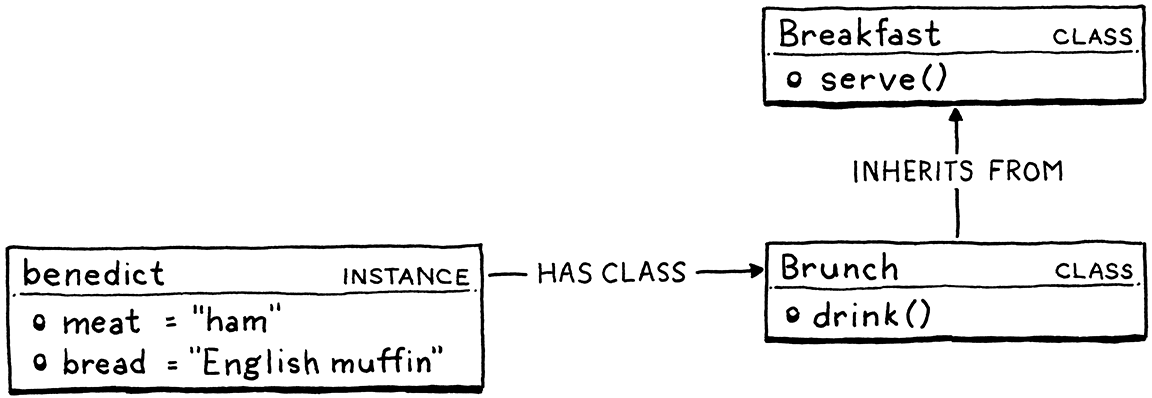
\includegraphics[width=\textwidth]{image/the-lox-language/class-lookup.png}
\end{figure}

基于原型的语言融合了这两个概念。这里只有对象——没有类,而且每个对象都可以包含状态和方法。对象之间可以直接继承(或者用原型语言的术语说是“委托”):

\begin{figure}[htbp]
  \centering
  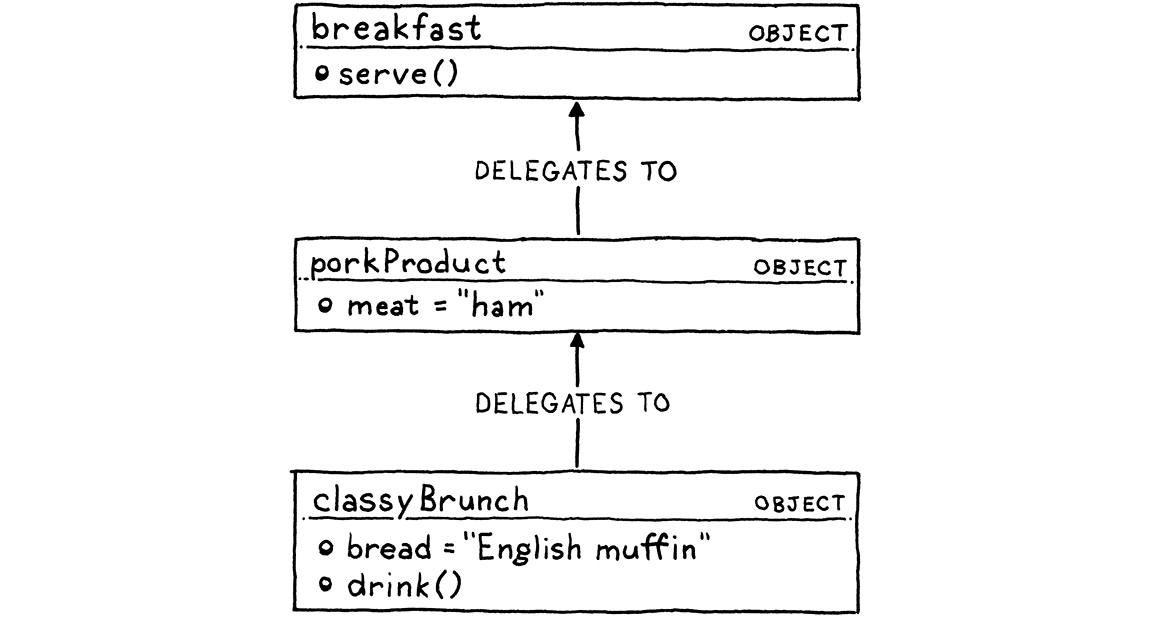
\includegraphics[width=\textwidth]{image/the-lox-language/prototype-lookup.png}
\end{figure}

这意味着原型语言在某些方面比类更基础。它们实现起来真的很整洁,因为它们很简单。另外,它们还可以表达很多不寻常的模式,而这些模式是类所不具备的。

但是我看过很多用原型语言写的代码——包括我自己设计的一些代码。你知道人们一般会怎么使用原型的强大功能和灵活性吗?...他们用它来重新发明类。

我不知道这是为什么,但人们自然而然地似乎更喜欢基于类的(经典?优雅?)风格。原型在语言中更简单,但它们似乎只是通过将复杂性推给用户来实现的。所以,对于Lox来说,我们将省去用户的麻烦,直接把类包含进去。

\subsection{Lox中的类}

理由已经说够了,来看看我们实际上拥有什么。在大多数语言中,类包含了一系列的特性。对于Lox,我选择了我认为最闪亮的一点。您可以像这样声明一个类及其方法:

\begin{code}{js}{}{}
class Breakfast {
  cook() {
    print "Eggs a-fryin'!";
  }

  serve(who) {
    print "Enjoy your breakfast, " + who + ".";
  }
}
\end{code}

类的主体包含其方法。它们看起来像函数声明,但没有fun关键字。当类声明生效时,Lox将创建一个类对象,并将其存储在以该类命名的变量中。就像函数一样,类在Lox中也是一等公民:

\begin{code}{js}{}{}
// Store it in variables.
var someVariable = Breakfast;

// Pass it to functions.
someFunction(Breakfast);
\end{code}

接下来,我们需要一种创建实例的方法。我们可以添加某种new关键字,但为了简单起见,在Lox中,类本身是实例的工厂函数。像调用函数一样调用一个类,它会生成一个自己的新实例:

\begin{code}{js}{}{}
var breakfast = Breakfast();
print breakfast; // "Breakfast instance".
\end{code}

\subsection{实例化和初始化}

只有行为的类不是非常有用。面向对象编程背后的思想是将行为和状态封装在一起。为此,您需要有字段。Lox和其他动态类型语言一样,允许您自由地向对象添加属性:

\begin{code}{js}{}{}
breakfast.meat = "sausage";
breakfast.bread = "sourdough";
\end{code}

如果一个字段不存在,那么对它进行赋值时就会先创建。

如果您想从方法内部访问当前对象上的字段或方法,可以使用this:

\begin{code}{js}{}{}
class Breakfast {
  serve(who) {
    print "Enjoy your " + this.meat + " and " +
        this.bread + ", " + who + ".";
  }

  // ...
}
\end{code}

在对象中封装数据的目的之一是确保对象在创建时处于有效状态。为此,你可以定义一个初始化器。如果您的类中包含一个名为init()的方法,则在构造对象时会自动调用该方法。传递给类的任何参数都会转发给它的初始化器:

\begin{code}{js}{}{}
class Breakfast {
  init(meat, bread) {
    this.meat = meat;
    this.bread = bread;
  }

  // ...
}

var baconAndToast = Breakfast("bacon", "toast");
baconAndToast.serve("Dear Reader");
// "Enjoy your bacon and toast, Dear Reader."
\end{code}

\subsection{继承}

在每一种面向对象的语言中,你不仅可以定义方法,而且可以在多个类或对象中重用它们。为此,Lox支持单继承。当你声明一个类时,你可以使用小于(<)操作符指定它继承的类:

\begin{code}{js}{}{}
class Brunch < Breakfast {
  drink() {
    print "How about a Bloody Mary?";
  }
}
\end{code}

这里,Brunch是\textbf{派生类}或\textbf{子类},而Breakfast是\textbf{基类}或\textbf{超类}。父类中定义的每个方法对其子类也可用:

\begin{code}{js}{}{}
var benedict = Brunch("ham", "English muffin");
benedict.serve("Noble Reader");
\end{code}

即使是init()方法也会被继承。在实践中,子类通常也想定义自己的init()方法。但还需要调用原始的初始化方法,以便超类能够维护其状态。我们需要某种方式能够调用自己实例上的方法,而无需触发实例自身的方法。

与Java中一样,您可以使用super:

\begin{code}{js}{}{}
class Brunch < Breakfast {
  init(meat, bread, drink) {
    super.init(meat, bread);
    this.drink = drink;
  }
}
\end{code}

这就是面向对象的内容。我尽量将功能设置保持在最低限度。本书的结构确实迫使我做了一个妥协。Lox不是一种纯粹的面向对象的语言。在真正的OOP语言中,每个对象都是一个类的实例,即使是像数字和布尔值这样的基本类型。

因为我们开始使用内置类型很久之后才会实现类,所以这一点很难实现。因此,从类实例的意义上说,基本类型的值并不是真正的对象。它们没有方法或属性。如果以后我想让Lox成为真正的用户使用的语言,我会解决这个问题。

\section{标准库}

我们快结束了,这就是整个语言,所剩下的就是“核心”或“标准”库——这是一组直接在解释器中实现的功能集,所有用户定义的行为都是建立在此之上。

这是Lox中最可悲的部分。它的标准库已经超过了极简主义,解决彻底的虚无主义。对于本书中的示例代码,我们只需要证明代码在运行,并且在做它应该做的事。为此,我们已经有了内置的print语句。

稍后,当我们开始优化时,我们将编写一些基准测试,看看执行代码需要多长时间。这意味着我们需要跟踪时间,因此我们将定义一个内置函数clock(),该函数会返回程序启动后的秒数。

嗯...就是这样。我知道,有点尴尬,对吧? 

如果您想将Lox变成一门实际可用的语言,那么您应该做的第一件事就是对其充实。字符串操作、三角函数、文件I/O、网络、扩展,甚至读取用户的输入都将有所帮助。但对于本书来说,我们不需要这些,而且加入这些也不会教给你任何有趣的东西,所以我把它省略了。

别担心,这门语言本身就有很多精彩的内容让我们忙个不停。

\section{挑战}

\begin{enumerate}
  \item 编写一些示例Lox程序并运行它们(您可以使用我的Lox实现)。试着想出我在这里没有详细说明的边界情况。它是否按照期望运行?为什么?
  \item 这种非正式的介绍留下了很多未说明的东西。列出几个关于语言语法和语义的开放问题。你认为答案应该是什么?
  \item Lox是一种很小的语言。您认为缺少哪些功能会使其不适用于实际程序? (当然,除了标准库。)
\end{enumerate}

\section{设计笔记:表达式和语句}

Lox既有表达式也有语句。有些语言省略了后者。相对地,它们将声明和控制流结构也视为表达式。这类“一切都是表达式”的语言往往具有函数式的血统,包括大多数Lisp、SML、Haskell、Ruby和CoffeeScript。

要做到这一点,对于语言中的每一个“类似于语句”的构造,你需要决定它所计算的值是什么。其中有些很简单:

\begin{itemize}
  \item if表达式的计算结果是所选分支的结果。同样,switch或其他多路分支的计算结果取决于所选择的情况。
  \item 变量声明的计算结果是变量的值。
  \item 块的计算结果是序列中最后一个表达式的结果。
\end{itemize}

有一些是比较复杂的。循环应该计算什么值?在CoffeeScript中,一个while循环计算结果为一个数组,其中包含了循环体中计算到的每个元素。这可能很方便,但如果你不需要这个数组,就会浪费内存。

您还必须决定这些类似语句的表达式如何与其他表达式组合,必须将它们放入语法的优先表中。例如,Ruby允许下面这种写法:

\begin{code}{ruby}{}{}
puts 1 + if true then 2 else 3 end + 4
\end{code}

这是你所期望的吗?这是你的用户所期望的吗?这对你如何设计“语句”的语法有什么影响?请注意,Ruby有一个显式的end关键字来表明if表达式结束。如果没有它,+4很可能会被解析为else子句的一部分。

把每个语句都转换成表达式会迫使你回答一些类似这样的复杂问题。作为回报,您消除了一些冗余。C语言中既有用于排序语句的块,以及用于排序表达式的逗号操作符。它既有if语句,也有?:条件操作符。如果在C语言中所有东西都是表达式,你就可以把它们统一起来。

取消了语句的语言通常还具有\textbf{隐式返回}的特点——函数自动返回其函数主体所计算得到的任何值,而不需要显式的return语法。对于小型函数和方法来说,这真的很方便。事实上,许多有语句的语言都添加了类似于=>的语法,以便能够定义函数体是计算单一表达式结果的函数。

但是让所有的函数以这种方式工作可能有点奇怪。即使你只是想让函数产生副作用,如果不小心,函数也可能会泄露返回值。但实际上,这些语言的用户并不觉得这是一个问题。

对于Lox,我在其中添加语句是出于朴素的原因。为了熟悉起见,我选择了一种类似于C的语法,而试图把现有的C语句语法像表达式一样解释,会变得非常快。

\part{树遍历解释器}

\chapter{扫描}

\epigraph{大干特工。每件值得做的事都值得反复去做。}{罗伯特}

任何编译器或解释器的第一步都是扫描。扫描器以一系列字符的形式接收原始源代码,并将其分组成一系列的块,我们称之为\textbf{标识}(词法单元)。这些是有意义的“单词”和“标点”,它们构成了语言的语法。

对于我们来说,扫描也是一个很好的起点,因为代码不是很难——相当于有很多分支的switch语句。这可以帮助我们在学习更后面有趣的部分之前进行热身。在本章结束时,我们将拥有一个功能齐全、速度快的扫描器,它可以接收任何一串Lox源代码,并产生标记,我们将在下一章把这些标记输入到解析器中。

\section{解释器框架}

由于这是我们的第一个真正的章节,在我们开始实际扫描代码之前,我们需要先勾勒出我们的解释器jlox的基本形态。在Java中,一切都是从一个类开始的。

\begin{code}{java}{}{lox/Lox.java,创建新文件}
package com.craftinginterpreters.lox;

import java.io.BufferedReader;
import java.io.IOException;
import java.io.InputStreamReader;
import java.nio.charset.Charset;
import java.nio.file.Files;
import java.nio.file.Paths;
import java.util.List;

public class Lox {
  public static void main(String[] args) throws IOException {
    if (args.length > 1) {
      System.out.println("Usage: jlox [script]");
      System.exit(64); 
    } else if (args.length == 1) {
      runFile(args[0]);
    } else {
      runPrompt();
    }
  }
}
\end{code}

把它贴在一个文本文件里,然后去把你的IDE或者Makefile或者其他工具设置好。我就在这里等你准备好。好了吗?好的!

Lox是一种脚本语言,这意味着它直接从源代码执行。我们的解释器支持两种运行代码的方式。如果从命令行启动jlox并为其提供文件路径,它将读取该文件并执行。

\begin{code}{java}{}{lox/Lox.java,添加到main()方法之后}
private static void runFile(String path) throws IOException {
  byte[] bytes = Files.readAllBytes(Paths.get(path));
  run(new String(bytes, Charset.defaultCharset()));
}
\end{code}

\begin{code}{java}{}{lox/Lox.java,添加到runFile()方法之后}
private static void runPrompt() throws IOException {
  InputStreamReader input = new InputStreamReader(System.in);
  BufferedReader reader = new BufferedReader(input);

  for (;;) { 
    System.out.print("> ");
    String line = reader.readLine();
    if (line == null) break;
    run(line);
  }
}
\end{code}

readLine()函数,顾名思义,读取用户在命令行上的一行输入,并返回结果。要终止交互式命令行应用程序,通常需要输入Control-D。这样做会向程序发出“文件结束”的信号。当这种情况发生时,readLine()就会返回null,所以我们检查一下是否存在null以退出循环。

交互式提示符和文件运行工具都是对这个核心函数的简单包装:

\begin{code}{java}{}{lox/Lox.java,添加到runPrompt()之后}
  private static void run(String source) {
    Scanner scanner = new Scanner(source);
    List<Token> tokens = scanner.scanTokens();

    // For now, just print the tokens.
    for (Token token : tokens) {
      System.out.println(token);
    }
  }
\end{code}

因为我们还没有写出解释器,所以这些代码还不是很有用,但这只是小步骤,你要明白?现在,它可以打印出我们即将完成的扫描器所返回的标记,这样我们就可以看到我们的解析是否生效。

\subsection{错误处理}

当我们设置东西的时候,另一个关键的基础设施是错误处理。教科书有时会掩盖这一点,因为这更多的是一个实际问题,而不是一个正式的计算机科学问题。但是,如果你关心的是如何制作一个真正可用的语言,那么优雅地处理错误是至关重要的。

我们的语言提供的处理错误的工具构成了其用户界面的很大一部分。当用户的代码在工作时,他们根本不会考虑我们的语言——他们的脑子里都是他们的程序。通常只有当程序出现问题时,他们才会注意到我们的实现。

当这种情况发生时,我们就需要向用户提供他们所需要的所有信息,让他们了解哪里出了问题,并引导他们慢慢达到他们想要去的地方。要做好这一点,意味着从现在开始,在解释器的整个实现过程中都要考虑错误处理。

\begin{code}{java}{}{lox/Lox.java,添加到run()方法之后}
static void error(int line, String message) {
    report(line, "", message);
  }

  private static void report(int line, String where,
                             String message) {
    System.err.println(
        "[line " + line + "] Error" + where + ": " + message);
    hadError = true;
  }
\end{code}

这个error()函数和其工具方法report()会告诉用户在某一行上发生了一些语法错误。这其实是最起码的,可以说你有错误报告功能。想象一下,如果你在某个函数调用中不小心留下了一个悬空的逗号,解释器就会打印出来:

\begin{code}{java}{}{}
Error: Unexpected "," somewhere in your code. Good luck finding it!
\end{code}

这种信息没有多大帮助。我们至少要给他们指出正确的方向。好一些的做法是指出开头和结尾一栏,这样他们就知道这一行的位置了。更好的做法是向用户显示违规的行,比如:

\begin{code}{java}{}{}
Error: Unexpected "," in argument list.

    15 | function(first, second,);
                               ^-- Here.
\end{code}

我很想在这本书里实现这样的东西,但老实说,这会引入很多繁琐的字符串操作代码。这些代码对用户来说非常有用,但在书中读起来并不友好,而且技术上也不是很有趣。所以我们还是只用一个行号。在你们自己的解释器中,请按我说的做,而不是按我做的做。

我们在Lox主类中坚持使用这个错误报告功能的主要原因就是因为那个hadError字段。它的定义在这里:

\begin{code}{java}{}{lox/Lox.java 在Lox类中添加}
public class Lox {
  static boolean hadError = false;
\end{code}

我们将以此来确保我们不会尝试执行有已知错误的代码。此外,它还能让我们像一个好的命令行工具那样,用一个非零的结束代码退出。

\begin{code}{java}{}{lox/Lox.java,在runFile()中添加}
    run(new String(bytes, Charset.defaultCharset()));
    
    // Indicate an error in the exit code.
    if (hadError) System.exit(65);
  }
\end{code}

我们需要在交互式循环中重置此标志。如果用户输入有误,也不应终止整个会话。

\begin{code}{java}{}{lox/Lox.java,在runPrompt()中添加}
      run(line);
      hadError = false;
    }
\end{code}

我把错误报告拉出来,而不是把它塞进扫描器和其他可能发生错误的阶段,还有另一个原因,是为了提醒您,把产生错误的代码和报告错误的代码分开是一个很好的工程实践。

前端的各个阶段都会检测到错误,但是它们不需要知道如何向用户展示错误。再一个功能齐全的语言实现中,可能有多种方式展示错误信息:在stderr,在IDE的错误窗口中,记录到文件,等等。您肯定不希望扫描器和解释器中到处充斥着这类代码。

理想情况下,我们应该有一个实际的抽象,即传递给扫描程序和解析器的某种ErrorReporter接口,这样我们就可以交换不同的报告策略。对于我们这里的简单解释器,我没有那样做,但我至少将错误报告代码移到了一个不同的类中。

有了一些基本的错误处理,我们的应用程序外壳已经准备好了。一旦我们有了一个带有scanTokens()方法的Scanner类,我们就可以开始运行它了。在我们开始之前,让我们更精确地了解什么是标记(tokens)。

\section{词素和标记(词法单元)}

下面是一行lox代码:

\begin{code}{js}{}{}
var language = "lox";
\end{code}

在这里,var是声明变量的关键字。“v-a-r”这三个字符的序列是有意义的。但如果我们从language中间抽出三个字母,比如“g-u-a”,它们本身并没有任何意义。

这就是词法分析的意义所在。我们的工作是扫描字符列表,并将它们归纳为具有某些含义的最小序列。每一组字符都被称为词素。在示例代码行中,词素是:

\begin{figure}[htbp]
  \centering
  
\includegraphics[width=\textwidth]{image/scanning/lexemes.png}
\end{figure}

词素只是源代码的原始子字符串。但是,在将字符序列分组为词素的过程中,我们也会发现了一些其他有用的信息。当我们获取词素并将其与其他数据捆绑在一起时,结果是一个标记(token,词法单元)。它包含一些有用的内容,比如:

\subsection{标记类型}

关键词是语言语法的一部分,所以解析器经常会有这样的代码:“如果下一个标记是while,那么就......”。这意味着解析器想知道的不仅仅是它有某个标识符的词素,而是它得到一个\textit{保留词},以及它是\textit{哪个}关键词。

解析器可以通过比较字符串对原始词素中的标记进行分类,但这样做很慢,而且有点难看。相反,在我们识别一个词素的时候,我们还要记住它代表的是哪种词素。我们为每个关键字、操作符、标点位和字面量都有不同的类型。

\begin{code}{java}{}{lox/TokenType.java,创建新文件}
package com.craftinginterpreters.lox;

enum TokenType {
  // Single-character tokens.
  LEFT_PAREN, RIGHT_PAREN, LEFT_BRACE, RIGHT_BRACE,
  COMMA, DOT, MINUS, PLUS, SEMICOLON, SLASH, STAR,

  // One or two character tokens.
  BANG, BANG_EQUAL,
  EQUAL, EQUAL_EQUAL,
  GREATER, GREATER_EQUAL,
  LESS, LESS_EQUAL,

  // Literals.
  IDENTIFIER, STRING, NUMBER,

  // Keywords.
  AND, CLASS, ELSE, FALSE, FUN, FOR, IF, NIL, OR,
  PRINT, RETURN, SUPER, THIS, TRUE, VAR, WHILE,

  EOF
}
\end{code}

\subsection{字面量}

字面量有对应词素——数字和字符串等。由于扫描器必须遍历文字中的每个字符才能正确识别,所以它还可以将值的文本表示转换为运行时对象,解释器后续将使用该对象。

\subsection{位置信息}

早在我宣讲错误处理的福音时,我们就看到,我们需要告诉用户错误发生在哪里。(用户)从这里开始定位问题。在我们的简易解释器中,我们只说明了标记出现在哪一行上,但更复杂的实现中还应该包括列位置和长度。

我们将所有这些数据打包到一个类中。

\begin{code}{java}{}{lox/Token.java,创建新文件}
package com.craftinginterpreters.lox;

class Token {
  final TokenType type;
  final String lexeme;
  final Object literal;
  final int line; 

  Token(TokenType type, String lexeme, Object literal, int line) {
    this.type = type;
    this.lexeme = lexeme;
    this.literal = literal;
    this.line = line;
  }

  public String toString() {
    return type + " " + lexeme + " " + literal;
  }
}
\end{code}

现在我们有了一个信息充分的对象,足以支撑解释器的所有后期阶段。

\section{正则语言和表达式}

既然我们已知道我们要输出的什么,那么,我们就开始吧。扫描器的核心是一个循环。从源码的第一个字符开始,扫描器计算出该字符属于哪个词素,并消费它和属于该词素的任何后续字符。当到达该词素的末尾时,扫描器会输出一个标记。

然后再循环一次,它又循环回来,从源代码中的下一个字符开始再做一次。它一直这样做,吃掉字符,偶尔,呃,排出标记,直到它到达输入的终点。

\begin{figure}[htbp]
  \centering
  
\includegraphics[width=\textwidth]{image/scanning/lexigator.png}
\end{figure}

在循环中,我们会查看一些字符,以确定它“匹配”的是哪种词素,这部分内容可能听起来很熟悉,但如果你知道正则表达式,你可以考虑为每一种词素定义一个regex,并使用这些regex来匹配字符。如果你了解正则表达式,你可以考虑为每一种词素定义一个regex,然后用来匹配字符。例如,Lox对标识符(变量名等)的规则与C语言相同。下面的regex可以匹配一个标识符:

\begin{code}{js}{}{}
[a-zA-Z_][a-zA-Z_0-9]*
\end{code}

如果你确实想到了正则表达式,那么你的直觉还是很深刻的。决定一门语言如何将字符分组为词素的规则被称为它的\textbf{词法语法}。在Lox中,和大多数编程语言一样,该语法的规则非常简单,可以将其归为\textbf{正则语言}。这里的正则和正则表达式中的“正则”是一样的含义。

如果你愿意,你可以非常精确地使用正则表达式来识别Lox的所有不同词组,而且还有一堆有趣的理论来支撑着为什么会这样以及它的意义。像Lex或Flex这样的工具就是专门为实现这一功能而设计的——向其中传入一些正则表达式,它可以为您提供完整的扫描器。

由于我们的目标是了解扫描器是如何工作的,所以我们不会把这个任务交给正则表达式。我们要亲自动手实现。

\section{Scanner类}

事不宜迟,我们先来建一个扫描器吧。

\begin{code}{java}{}{lox/Scanner.java,创建新文件}
package com.craftinginterpreters.lox;

import java.util.ArrayList;
import java.util.HashMap;
import java.util.List;
import java.util.Map;

import static com.craftinginterpreters.lox.TokenType.*; 

class Scanner {
  private final String source;
  private final List<Token> tokens = new ArrayList<>();

  Scanner(String source) {
    this.source = source;
  }
}
\end{code}

我们将原始的源代码存储为一个简单的字符串,并且我们已经准备了一个列表来保存扫描时产生的标记。前面提到的循环看起来类似于:

\begin{code}{java}{}{lox/Scanner.java,方法Scanner()后添加}
  List<Token> scanTokens() {
    while (!isAtEnd()) {
      // We are at the beginning of the next lexeme.
      start = current;
      scanToken();
    }

    tokens.add(new Token(EOF, "", null, line));
    return tokens;
  }
\end{code}

扫描器通过自己的方式遍历源代码,添加标记,直到遍历完所有字符。然后,它在最后附加一个的“end of file”标记。严格意义上来说,这并不是必须的,但它可以使我们的解析器更加干净。

这个循环依赖于几个字段来跟踪扫描器在源代码中的位置。

\begin{code}{java}{2-4}{lox/Scanner.java,在Scanner类中添加}
  private final List<Token> tokens = new ArrayList<>();
  private int start = 0;
  private int current = 0;
  private int line = 1;

  Scanner(String source) {
\end{code}

start和current字段是指向字符串的偏移量。start字段指向被扫描的词素中的第一个字符,current字段指向当前正在处理的字符。line字段跟踪的是current所在的源文件行数,这样我们产生的标记就可以知道其位置。

然后,我们还有一个辅助函数,用来告诉我们是否已消费完所有字符。

\begin{code}{java}{}{lox/Scanner.java在scanTokens()方法之后添加}
  private boolean isAtEnd() {
    return current >= source.length();
  }
\end{code}

\section{识别词素}

在每一次循环中,我们会扫描一个标记。这是扫描器真正的核心。让我们先从简单情况开始。想象一下,如果每个词素只有一个字符长。您所需要做的就是消费下一个字符并为其选择一个标记类型。在Lox中有一些词素只包含一个字符,所以我们从这些词素开始。

\begin{code}{java}{}{lox/Scanner.java添加到scanTokens()方法之后}
private void scanToken() {
    char c = advance();
    switch (c) {
      case '(': addToken(LEFT_PAREN); break;
      case ')': addToken(RIGHT_PAREN); break;
      case '{': addToken(LEFT_BRACE); break;
      case '}': addToken(RIGHT_BRACE); break;
      case ',': addToken(COMMA); break;
      case '.': addToken(DOT); break;
      case '-': addToken(MINUS); break;
      case '+': addToken(PLUS); break;
      case ';': addToken(SEMICOLON); break;
      case '*': addToken(STAR); break; 
    }
  }
\end{code}

同样,我们也需要一些辅助方法。

\begin{code}{java}{}{lox/Scanner.java,添加到isAtEnd()方法后}
  private char advance() {
    current++;
    return source.charAt(current - 1);
  }

  private void addToken(TokenType type) {
    addToken(type, null);
  }

  private void addToken(TokenType type, Object literal) {
    String text = source.substring(start, current);
    tokens.add(new Token(type, text, literal, line));
  }
\end{code}

advance()方法获取源文件中的下一个字符并返回它。advance()用于处理输入,addToken()则用于输出。该方法获取当前词素的文本并为其创建一个新标记。我们马上会使用另一个重载方法来处理带有字面值的标记。

\subsection{词法错误}

在我们深入探讨之前,我们先花一点时间考虑一下词法层面的错误。如果用户抛入解释器的源文件中包含一些Lox中不使用的字符——如@\#\^,会发生什么?现在,这些字符被默默抛弃了。它们没有被Lox语言使用,但是不意味着解释器可以假装它们不存在。相反,我们应该报告一个错误:

\begin{code}{java}{}{lox/Scanner.java 在scanToken()方法中添加}
      case '*': addToken(STAR); break; 

      default:
        Lox.error(line, "Unexpected character.");
        break;
    }
\end{code}

注意,错误的字符仍然会被前面调用的advance()方法消费。这一点很重要,这样我们就不会陷入无限循环了。

另请注意,我们一直在扫描。程序稍后可能还会出现其他错误。如果我们能够一次检测出尽可能多的错误,将为我们的用户带来更好的体验。否则,他们会看到一个小错误并修复它,但是却出现下一个错误,不断重复这个过程。语法错误“打地鼠”一点也不好玩。

(别担心。因为hadError进行了赋值,我们永远不会尝试执行任何代码,即使程序在继续运行并扫描代码文件的其余部分。)

\subsection{运算符}

我们的单字符词素已经生效了,但是这不能涵盖Lox中的所有操作符。比如!?这是单字符,对吧?有时候是的,但是如果下一个字符是等号,那么我们应该改用!=词素。注意,这里的!和=\textit{不是}两个独立的运算符。在Lox中,你不能写! =来表示不等操作符。这就是为什么我们需要将!=作为单个词素进行扫描。同样地,<、>和=都可以与后面跟随的=来组合成其他相等和比较操作符。

对于所有这些情况,我们都需要查看第二个字符。

\begin{code}{java}{}{lox/Scanner.java,在scanToken()方法中添加}
      case '*': addToken(STAR); break; 
      case '!':
        addToken(match('=') ? BANG_EQUAL : BANG);
        break;
      case '=':
        addToken(match('=') ? EQUAL_EQUAL : EQUAL);
        break;
      case '<':
        addToken(match('=') ? LESS_EQUAL : LESS);
        break;
      case '>':
        addToken(match('=') ? GREATER_EQUAL : GREATER);
        break;
      default:
\end{code}

这些分支中使用了下面的新方法:

\begin{code}{java}{}{lox/Scanner.java 添加到scanToken()方法后}
  private boolean match(char expected) {
    if (isAtEnd()) return false;
    if (source.charAt(current) != expected) return false;

    current++;
    return true;
  }
\end{code}

这就像一个有条件的advance()。只有当前字符是我们正在寻找的字符时,我们才会消费。

使用match(),我们分两个阶段识别这些词素。例如,当我们得到!时,我们会跳转到它的case分支。这意味着我们知道这个词素是以!开始的。然后,我们查看下一个字符,以确认词素是一个!=还是仅仅是一个!。

\section{更长的词素}

我们还缺少一个操作符:表示除法的/。这个字符需要一些特殊处理,因为注释也是以斜线开头的。

\begin{code}{java}{}{lox/Scanner.java,在scanToken()方法中添加}
      break;
      case '/':
        if (match('/')) {
          // A comment goes until the end of the line.
          while (peek() != '\n' && !isAtEnd()) advance();
        } else {
          addToken(SLASH);
        }
        break;
      default:
\end{code}

这与其它的双字符运算符是类似的,区别在于我们找到第二个/时,还没有结束本次标记。相反,我们会继续消费字符直至行尾。

这是我们处理较长词素的一般策略。当我们检测到一个词素的开头后,我们会分流到一些特定于该词素的代码,这些代码会不断地消费字符,直到结尾。

我们又有了一个辅助函数:

\begin{code}{java}{}{lox/Scanner.java,在match()方法后添加}
  private char peek() {
    if (isAtEnd()) return '\0';
    return source.charAt(current);
  }
\end{code}

这有点像advance()方法,只是不会消费字符。这就是所谓的\textbf{lookahead(前瞻)}。因为它只关注当前未消费的字符,所以我们有\textit{一个前瞻字符}。一般来说,数字越小,扫描器运行速度就越快。词法语法的规则决定了我们需要前瞻多少字符。幸运的是,大多数广泛使用的语言只需要提前一到两个字符。

注释是词素,但是它们没有含义,而且解析器也不想要处理它们。所以,我们达到注释末尾后,\textit{不会}调用addToken()方法。当我们循环处理下一个词素时,start已经被重置了,注释的词素就消失在一阵烟雾中了。

既然如此,现在正好可以跳过其它那些无意义的字符了:换行和空格。

\begin{code}{java}{}{lox/Scanner.java,在scanToken()方法中添加}
        break;
      case ' ':
      case '\r':
      case '\t':
        // Ignore whitespace.
        break;

      case '\n':
        line++;
        break;
      default:
        Lox.error(line, "Unexpected character.");
\end{code}

当遇到空白字符时,我们只需回到扫描循环的开头。这样就会在空白字符之后开始一个新的词素。对于换行符,我们做同样的事情,但我们也会递增行计数器。(这就是为什么我们使用peek()而不是match()来查找注释结尾的换行符。我们到这里希望能读取到换行符,这样我们就可以更新行数了)

我们的扫描器越来越聪明了。它可以处理相当自由形式的代码,如:

\begin{code}{java}{}{}
// this is a comment
(( )){} // grouping stuff
!*+-/=<> <= == // operators
\end{code}

\subsection{字符串字面量}

现在我们对长词素已经很熟悉了,我们可以开始处理字面量了。我们先处理字符串,因为字符串总是以一个特定的字符"开头。

\begin{code}{java}{}{lox/Scanner.java,在scanToken()方法中添加}
        break;
      case '"': string(); break;
      default:
\end{code}

这里会调用:

\begin{code}{java}{}{lox/Scanner.java,在scanToken()方法之后添加}
  private void string() {
    while (peek() != '"' && !isAtEnd()) {
      if (peek() == '\n') line++;
      advance();
    }

    if (isAtEnd()) {
      Lox.error(line, "Unterminated string.");
      return;
    }

    // The closing ".
    advance();

    // Trim the surrounding quotes.
    String value = source.substring(start + 1, current - 1);
    addToken(STRING, value);
  }
\end{code}

与注释类似,我们会一直消费字符,直到"结束该字符串。如果输入内容耗尽,我们也会进行优雅的处理,并报告一个对应的错误。

没有特别的原因,Lox支持多行字符串。这有利有弊,但禁止换行比允许换行更复杂一些,所以我把它们保留了下来。这意味着当我们在字符串内遇到新行时,我们也需要更新line值。

最后,还有一个有趣的地方就是当我们创建标记时,我们也会产生实际的字符串值,该值稍后将被解释器使用。这里,值的转换只需要调用substring()剥离前后的引号。如果Lox支持转义序列,比如\\n,我们会在这里取消转义。

\subsection{数字字面量}

在Lox中,所有的数字在运行时都是浮点数,但是同时支持整数和小数字面量。一个数字字面量就是一系列数位,后面可以跟一个.和一或多个尾数。

\begin{code}{java}{}{}
1234
12.34
\end{code}

我们不允许小数点处于最开始或最末尾,所以下面的格式是不正确的:

\begin{code}{java}{}{}
.1234
1234.
\end{code}

我们可以很容易地支持前者,但为了保持简单,我把它删掉了。如果我们要允许对数字进行方法调用,比如123.sqrt(),后者会变得很奇怪。

为了识别数字词素的开头,我们会寻找任何一位数字。为每个十进制数字添加case分支有点乏味,所以我们直接在默认分支中进行处理。

\begin{code}{java}{2-6}{lox/Scanner.java,在scanToken()方法中替换1行:}
      default:
        if (isDigit(c)) {
          number();
        } else {
          Lox.error(line, "Unexpected character.");
        }
        break;
\end{code}

这里依赖下面的小工具函数:

\begin{code}{java}{}{lox/Scanner.java,在peek()方法之后添加}
  private boolean isDigit(char c) {
    return c >= '0' && c <= '9';
  } 
\end{code}

一旦我们知道当前在处理数字,我们就分支进入一个单独的方法消费剩余的字面量,跟字符串的处理类似。

\begin{code}{java}{}{lox/Scanner.java,在scanToken()方法后添加}
  private void number() {
    while (isDigit(peek())) advance();

    // Look for a fractional part.
    if (peek() == '.' && isDigit(peekNext())) {
      // Consume the "."
      advance();

      while (isDigit(peek())) advance();
    }

    addToken(NUMBER,
        Double.parseDouble(source.substring(start, current)));
  }
\end{code}

我们在字面量的整数部分中尽可能多地获取数字。然后我们寻找小数部分,也就是一个小数点(.)后面至少跟一个数字。如果确实有小数部分,同样地,我们也尽可能多地获取数字。

在定位到小数点之后需要前瞻两个字符,因为我们只有确认其\textit{后}有数字才会消费.。所以我们添加了:

\begin{code}{java}{}{lox/Scanner.java,在peek()方法后添加}
  private char peekNext() {
    if (current + 1 >= source.length()) return '\0';
    return source.charAt(current + 1);
  }
\end{code}

最后,我们将词素转换为其对应的数值。我们的解释器使用Java的Double类型来表示数字,所以我们创建一个该类型的值。我们使用Java自带的解析方法将词素转换为真正的Java double。我们可以自己实现,但是,说实话,除非你想为即将到来的编程面试做准备,否则不值得你花时间。

剩下的词素是Boolean和nil,但我们把它们作为关键字来处理,这样我们就来到了......

\section{保留字和标识符}

我们的扫描器基本完成了,词法语法中还需要实现的部分仅剩标识符及其近亲——保留字。你也许会想,我们可以采用与处理<=等多字符操作符时相同的方法来匹配关键字,如or。

\begin{code}{java}{}{}
case 'o':
  if (peek() == 'r') {
    addToken(OR);
  }
  break;
\end{code}

考虑一下,如果用户将变量命名为orchid会发生什么?扫描器会先看到前面的两个字符,然后立刻生成一个or标记。这就涉及到了一个重要原则,叫作\textbf{maximal munch}(最长匹配)。当两个语法规则都能匹配扫描器正在处理的一大块代码时,\textit{哪个规则相匹配的字符最多,就使用哪个规则}。

该规则规定,如果我们可以将orchid匹配为一个标识符,也可以将or匹配为一个关键字,那就采用第一种结果。这也就是为什么我们在前面会默认为,<=应该识别为单一的<=标记,而不是<后面跟了一个=。

最大匹配原则意味着,我们只有扫描完一个可能是标识符的片段,才能确认是否一个保留字。毕竟,保留字也是一个标识符,只是一个已经被语言要求为自己所用的标识符。这也是\textbf{保留字}一词的由来。

所以我们首先假设任何以字母或下划线开头的词素都是一个标识符。

\begin{code}{java}{4-5}{lox/Scanner.java,在scanToken()中添加代码}
        default:
        if (isDigit(c)) {
          number();
        } else if (isAlpha(c)) {
          identifier();
        } else {
          Lox.error(line, "Unexpected character.");
        }
\end{code}

其它代码如下:

\begin{code}{java}{}{lox/Scanner.java,在scanToken()方法之后添加}
  private void identifier() {
    while (isAlphaNumeric(peek())) advance();

    addToken(IDENTIFIER);
  }
\end{code}

通过以下辅助函数来定义:

\begin{code}{java}{}{lox/Scanner.java,在peekNext()方法之后添加}
  private boolean isAlpha(char c) {
    return (c >= 'a' && c <= 'z') ||
           (c >= 'A' && c <= 'Z') ||
            c == '_';
  }

  private boolean isAlphaNumeric(char c) {
    return isAlpha(c) || isDigit(c);
  }
\end{code}

这样标识符就开始工作了。为了处理关键字,我们要查看标识符的词素是否是保留字之一。如果是,我们就使用该关键字特有的标记类型。我们在map中定义保留字的集合。

\begin{code}{java}{}{lox/Scanner.java,在Scanner类中添加}
  private static final Map<String, TokenType> keywords;

  static {
    keywords = new HashMap<>();
    keywords.put("and",    AND);
    keywords.put("class",  CLASS);
    keywords.put("else",   ELSE);
    keywords.put("false",  FALSE);
    keywords.put("for",    FOR);
    keywords.put("fun",    FUN);
    keywords.put("if",     IF);
    keywords.put("nil",    NIL);
    keywords.put("or",     OR);
    keywords.put("print",  PRINT);
    keywords.put("return", RETURN);
    keywords.put("super",  SUPER);
    keywords.put("this",   THIS);
    keywords.put("true",   TRUE);
    keywords.put("var",    VAR);
    keywords.put("while",  WHILE);
  }
\end{code}

接下来,在我们扫描到标识符之后,要检查是否与map中的某些项匹配。

\begin{code}{java}{3-6}{lox/Scanner.java,在identifier()方法中替换1行:}
    while (isAlphaNumeric(peek())) advance();

    String text = source.substring(start, current);
    TokenType type = keywords.get(text);
    if (type == null) type = IDENTIFIER;
    addToken(type);
  }
\end{code}

如果匹配的话,就使用关键字的标记类型。否则,就是一个普通的用户定义的标识符。

至此,我们就有了一个完整的扫描器,可以扫描整个Lox词法语法。启动REPL,输入一些有效和无效的代码。它是否产生了你所期望的词法单元?试着想出一些有趣的边界情况,看看它是否能正确地处理它们。

\section{挑战}

\begin{enumerate}
  \item Python和Haskell的语法不是\textit{正则的}。这是什么意思,为什么不是呢?
  \begin{itemize}
    \item Python和Haskell都采用了对缩进敏感的语法,所以它们必须将缩进级别的变动识别为词法标记。这样做需要比较连续行的开头空格数量,这是使用常规语法无法做到的。
  \end{itemize}
  \item 除了分隔标记——区分print foo和printfoo——空格在大多数语言中并没有什么用处。在CoffeeScript、Ruby和C预处理器中的一些隐秘的地方,空格确实会影响代码解析方式。在这些语言中,空格在什么地方,会有什么影响?
  \item 我们这里的扫描器和大多数扫描器一样,会丢弃注释和空格,因为解析器不需要这些。什么情况下你会写一个不丢弃这些的扫描器?它有什么用呢?
  \item 为Lox扫描器增加对C样式/ * ... * /屏蔽注释的支持。确保要处理其中的换行符。考虑允许它们嵌套,增加对嵌套的支持是否比你预期的工作更多?为什么?
\end{enumerate}

\section{设计笔记:隐藏的分号}

现在的程序员已经被越来越多的语言选择宠坏了,对语法也越来越挑剔。他们希望自己的代码看起来干净、现代化。几乎每一种新语言都会放弃一个小的语法点(一些古老的语言,比如BASIC从来没有过),那就是将;作为显式的语句结束符。

相对地,它们将“有意义的”换行符看作是语句结束符。这里所说的“有意义的”是有挑战性的部分。尽管\textit{大多数的}语句都是在同一行,但有时你需要将一个语句扩展到多行。这些混杂的换行符不应该被视作结束符。

大多数明显的应该忽略换行的情况都很容易发现,但也有少数讨厌的情况:

\begin{itemize}
  \item 返回值在下一行:

  \begin{code}{js}{}{}
  if (condition) return
  "value"
  \end{code}

  “value”是要返回的值吗?还是说我们有一个空的return语句,后面跟着包含一个字符串字面量的表达式语句。

  \item 下一行中有带圆括号的表达式:

  \begin{code}{js}{}{}
  func
  (parenthesized)
  \end{code}

  这是一个对func(parenthesized)的调用,还是两个表达式语句,一个用于func,一个用于圆括号表达式?

  \item “-”号在下一行:

  \begin{code}{js}{}{}
  first
  -second
  \end{code}

  这是一个中缀表达式——first - second,还是两个表达式语句,一个是first,另一个是对second取负?

在所有这些情况下,无论是否将换行符作为分隔符,都会产生有效的代码,但可能不是用户想要的代码。在不同的语言中,有各种不同的规则来决定哪些换行符是分隔符。下面是几个例子:

  \item Lua完全忽略了换行符,但是仔细地控制了它的语法,因此在大多数情况下,语句之间根本不需要分隔符。这段代码是完全合法的:

  \begin{code}{lua}{}{}
  a = 1 b = 2
  \end{code}

  Lua要求return语句是一个块中的最后一条语句,从而避免return问题。如果在关键字end之前、return之后有一个值,这个值\textit{必须}是用于return。对于其他两种情况来说,Lua允许显式的;并且期望用户使用它。在实践中,这种情况基本不会发生,因为在小括号或一元否定表达式语句中没有任何意义。

  \item Go会处理扫描器中的换行。如果在词法单元之后出现换行,并且该词法标记是已知可能结束语句的少数标记类型之一,则将换行视为分号,否则就忽略它。Go团队提供了一个规范的代码格式化程序gofmt,整个软件生态系统非常热衷于使用它,这确保了常用样式的代码能够很好地遵循这个简单的规则。

  \item Python将所有换行符都视为有效,除非在行末使用明确的反斜杠将其延续到下一行。但是,括号(()、[]或{})内的任何换行都将被忽略。惯用的代码风格更倾向于后者。

  这条规则对Python很有效,因为它是一种高度面向语句的语言。特别是,Python的语法确保了语句永远不会出现在表达式内。C语言也是如此,但许多其他有lambda或函数字面语法的语言则不然。

  举一个JavaScript中的例子:

  \begin{code}{js}{}{}
  console.log(function() {
    statement();
  });
  \end{code}

  这里,console.log()\textit{表达式}包含一个函数字面量,而这个函数字面量又包含statement();\textit{语句}。

  如果要求\textit{进入}一个嵌套在括号内的语句中,并且要求其中的换行是有意义的,那么Python将需要一套不同的隐式连接行的规则。

  \item JavaScript的“自动分号插入”规则才是真正的奇葩。其他语言认为大多数换行符都是有意义的,只有少数换行符在多行语句中应该被忽略,而JS的假设恰恰相反。它将所有的换行符都视为无意义的空白,除非遇到解析错误。如果遇到了,它就会回过头来,尝试把之前的换行变成分号,以期得到正确的语法。

  如果我完全详细地介绍它是如何工作的,那么这个设计说明就会变成一篇设计檄文,更不用说JavaScript的“解决方案”从各种角度看都是个坏主意。真是一团糟。许多风格指南要求在每条语句后都显式地使用分号,尽管理论上该语言允许您省略它们,但JavaScript是我所知道的唯一一种(省略分号的)语言。
\end{itemize}

如果您要设计一种新的语言,则几乎可以肯定应该避免使用显式的语句终止符。程序员和其他人类一样是时尚的动物,分号和ALL CAPS KEYWORDS(全大写关键字)一样已经过时了。只是要确保您选择了一套适用于您语言的特定语法和习语的规则即可。不要重蹈JavaScript的覆辙。

\chapter{表示代码}

\epigraph{对于森林中的居民来说,几乎每一种树都有它的声音和特点。}{哈代}

在上一章中,我们以字符串形式接收原始源代码,并将其转换为一个稍高级别的表示:一系列词法标记。我们在下一章中要编写的解析器,会将这些词法标记再次转换为更丰富、更复杂的表示形式。

在我们能够输出这种表示形式之前,我们需要先对其进行定义。这就是本章的主题。在这一过程中,我们将围绕形式化语法进行一些理论讲解,感受函数式编程和面向对象编程的区别,会介绍几种设计模式,并进行一些元编程。

在做这些事情之前,我们先关注一下主要目标——代码的表示形式。它应该易于解析器生成,也易于解释器使用。如果您还没有编写过解析器或解释器,那么这样的需求描述并不能很好地说明问题。也许你的直觉可以帮助你。当你扮演一个\textit{人类}解释器的角色时,你的大脑在做什么?你如何在心里计算这样的算术表达式:

\begin{code}{js}{}{}
1 + 2 * 3 - 4
\end{code}

因为你已经理解了操作的顺序——以前的“Please Excuse My Dear Aunt Sally”之类,你知道乘法在加减操作之前执行。有一种方法可以将这种优先级进行可视化,那就是使用树。叶子节点是数字,内部节点是运算符,它们的每个操作数都对应一个分支。

要想计算一个算术节点,你需要知道它的子树的数值,所以你必须先计算子树的结果。这意味着要从叶节点一直计算到根节点——\textit{后序}遍历:

\begin{figure}[htbp]
  \centering
  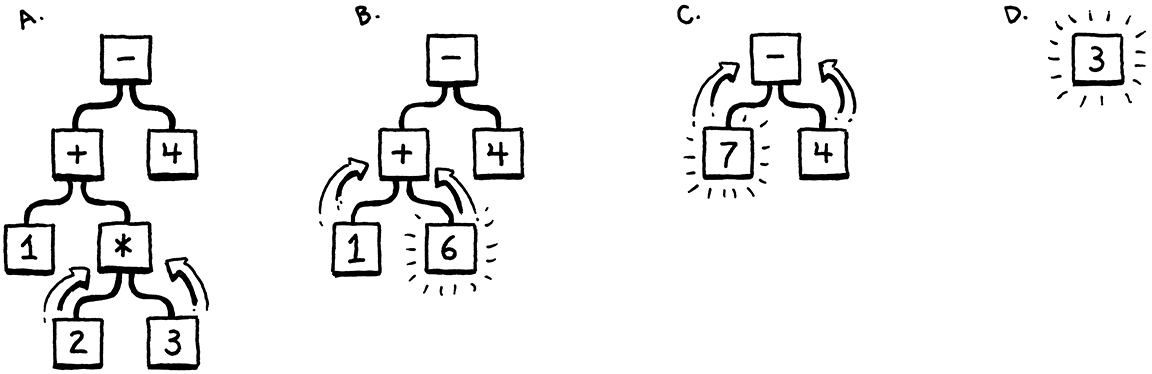
\includegraphics[width=\textwidth]{image/representing-code/tree-evaluate.png}
\end{figure}

\begin{itemize}
  \item A. 从完整的树开始,先计算最下面的操作2*3;
  \item B. 现在计算+;
  \item C. 接下来,计算-;
  \item D. 最终得到答案。
\end{itemize}

如果我给你一个算术表达式,你可以很容易地画出这样的树;给你一棵树,你也可以毫不费力地进行计算。因此,从直观上看,我们的代码的一种可行的表示形式是一棵与语言的语法结构(运算符嵌套)相匹配的树。

那么我们需要更精确地了解这个语法是什么。就像上一章的词法词法一样,围绕句法语法也有一大堆理论。我们要比之前处理扫描时投入更多精力去研究这个理论,因为它在整个解释器的很多地方都是一个有用的工具。我们先从乔姆斯基谱系中往上升一级......

\section{上下文无关语法}

在上一章中,我们用来定义词法语法(字符如何被分组为词法标记的规则)的形式体系,被称为\textit{正则语言}。这对于我们的扫描器来说没什么问题,因为它输出的是一个扁平的词法标记序列。但正则语言还不够强大,无法处理可以任意深度嵌套的表达式。

我们还需要一个更强大的工具,就是上下文无关语法(\textbf{context-free grammar},CFG)。它是形式化语法的工具箱中下一个最重的工具。一个形式化语法需要一组原子片段,它称之为“alphabet(字母表)”。然后它定义了一组(通常是无限的)“strings(字符串)”,这些字符串“包含”在语法中。每个字符串都是字母表中“letters(字符)”的序列。

我这里使用引号是因为当你从词法转到文法语法时,这些术语会让你有点困惑。在我们的扫描器词法中,alphabet(字母表)由单个字符组成,strings(字符串)是有效的词素(粗略的说,就是“单词”)。在现在讨论的文法语法中,我们处于一个不同的粒度水平。现在,字母表中的一个“letters(字符)”是一个完整的词法标记,而“strings(字符串)”是一个词法标记系列——一个完整的表达式。

嗯,使用表格可能更有助于理解:

\begin{center}
  \begin{tabular}{ |c|c|c|c| } 
   \hline
   术语 &  & 词法 & 语法 \\
   \hline 
   字母表 & $\rightarrow$ & 字符 & 词法标记 \\ 
   字符串 & $\rightarrow$ & 词素或词法标记 & 表达式 \\
   实现 & $\rightarrow$ & 扫描器 & 解析器 \\ 
   \hline
  \end{tabular}
\end{center}

形式化语法的工作是指定哪些字符串有效,哪些无效。如果我们要为英语句子定义一个语法,“eggs are tasty for breakfast”会包含在语法中,但“tasty breakfast for are eggs”可能不会。

\subsection{语法规则}

我们如何写下一个包含无限多有效字符串的语法?我们显然无法一一列举出来。相反,我们创建了一组有限的规则。你可以把它们想象成一场你可以朝两个方向“玩”的游戏。

如果你从规则入手,你可以用它们\textit{生成}语法中的字符串。以这种方式创建的字符串被称为\textbf{推导式}(派生式),因为每个字符串都是从语法规则中\textit{推导}出来的。在游戏的每一步中,你都要选择一条规则,然后按照它告诉你的去做。围绕形式化语法的大部分语言都倾向这种方式。规则被称为\textbf{生成式},因为它们生成了语法中的字符串。

上下文无关语法中的每个生成式都有一个\textbf{头部}(其名称)和描述其生成内容的\textbf{主体}。在纯粹的形式上看,主体只是一系列符号。符号有两种:

\begin{itemize}
  \item \textbf{终结符}是语法字母表中的一个字母。你可以把它想象成一个字面值。在我们定义的语法中,终止符是独立的词素——来自扫描器的词法标记,比如if或1234。这些词素被称为“终止符”,表示“终点”,因为它们不会导致游戏中任何进一步的 "动作"。你只是简单地产生了那一个符号。
  \item 非终止符是对语法中另一条规则的命名引用。它的意思是“执行那条规则,然后将它产生的任何内容插入这里”。这样,语法就构成了。
\end{itemize}

还有最后一个细节:你可以有多个同名的规则。当你遇到一个该名字的非终止符时,你可以为它选择任何一条规则,随您喜欢。

为了让这个规则具体化,我们需要一种方式来写下这些生成规则。人们一直试图将语法具体化,可以追溯到Pāṇini的\textit{Ashtadhyayi},他在几千年前编纂了梵文语法。直到约翰-巴科斯(John Backus)和公司需要一个声明ALGOL 58的符号,并提出了巴科斯范式(\textbf{BNF}),才有了很大的进展。从那时起,几乎每个人都在使用BNF的某种变形,并根据自己的需要进行了调整。

我试图提出一个简单的形式。 每个规则都是一个名称,后跟一个箭头($\rightarrow$),后跟一系列符号,最后以分号(;)结尾。终止符是带引号的字符串,非终止符是小写的单词。

以此为基础,下面是一个早餐菜单语法:

\begin{ebnf}
breakfast \quad & \rightarrow \quad protein \quad \mathtt{"}with\mathtt{"} \quad breakfast \quad \mathtt{"}on \; the \; side\mathtt{"} \quad ; \\
breakfast \quad & \rightarrow \quad protein \quad ; \\
breakfast \quad & \rightarrow \quad bread \quad ; \\
\\
protein  \quad & \rightarrow \quad crispiness \quad \mathtt{"}crispy\mathtt{"} \quad \mathtt{"}bacon\mathtt{"} \quad ; \\
protein  \quad & \rightarrow \quad \mathtt{"}sausage\mathtt{"} \quad ; \\
protein  \quad & \rightarrow \quad cooked \quad \mathtt{"}eggs\mathtt{"} \quad ; \\
\\
crispiness \quad & \rightarrow \quad \mathtt{"}really\mathtt{"} \quad ; \\
crispiness \quad & \rightarrow \quad \mathtt{"}really\mathtt{"} \quad crispiness \quad ; \\
\\
cooked \quad & \rightarrow \quad \mathtt{"}scrambled\mathtt{"} \quad ; \\
cooked \quad & \rightarrow \quad \mathtt{"}poached\mathtt{"} \quad ; \\
cooked \quad & \rightarrow \quad \mathtt{"}fried\mathtt{"} \quad ; \\
\\
bread \quad & \rightarrow \quad \mathtt{"}toast\mathtt{"} \quad; \\
bread \quad & \rightarrow \quad \mathtt{"}biscuits\mathtt{"} \quad ; \\
bread \quad & \rightarrow \quad \mathtt{"}English \; muffin\mathtt{"} \quad ;
\end{ebnf}

我们可以使用这个语法来随机生成早餐。我们来玩一轮,看看它是如何工作的。按照老规矩,游戏从语法中的第一个规则开始,这里是breakfast。它有三个生成式,我们随机选择第一个。我们得到的字符串是这样的:

\begin{tcolorbox}
protein "with" breakfast "on the side"
\end{tcolorbox}

我们需要展开第一个非终止符,protein,所有我们要选择它对应的一个生成式。我们选:

\begin{tcolorbox}
protein $\rightarrow$ cooked "eggs" ;
\end{tcolorbox}

接下来,我们需要cooked的生成式,我们选择“poached”。这是一个终止符,我们加上它。现在我们的字符串是这样的:

\begin{tcolorbox}
"poached" "eggs" "with" breakfast "on the side"
\end{tcolorbox}

下一个非终止符还是breakfast,我们开始选择的breakfast生成式递归地指向了breakfast规则。语法中的递归是一个很好的标志,表明所定义的语言是上下文无关的,而不是正则的。特别是,递归非终止符两边都有生成式的递归,意味着语言不是正则的。

我们可以不断选择breakfast的第一个生成式,以做出各种各样的早餐:“bacon with sausage with scrambled eggs with bacon......”,【存疑,按照规则设置,这里应该不会出现以bacon开头的字符串,原文可能有误】但我们不会这样做。这一次我们选择bread。有三个对应的规则,每个规则只包含一个终止符。我们选“English muffin”。

这样一来,字符串中的每一个非终止符都被展开了,直到最后只包含终止符,我们就剩下:

\begin{figure}[htbp]
  \centering
  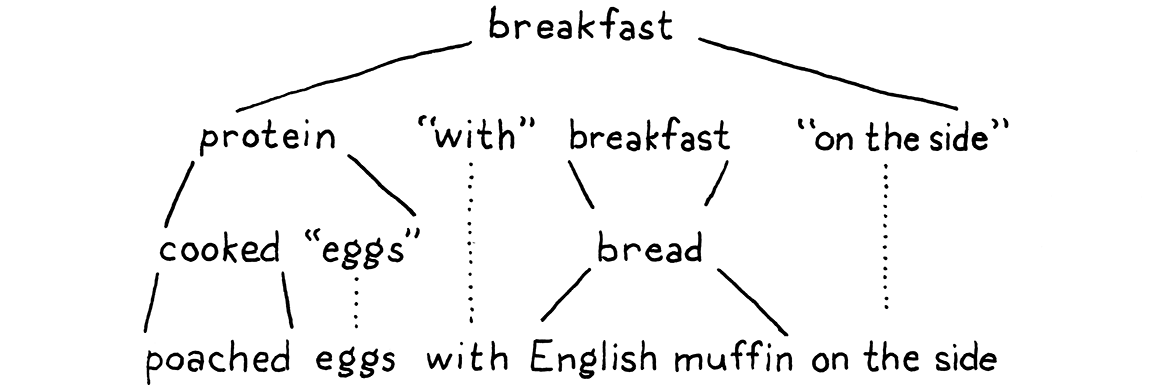
\includegraphics[width=\textwidth]{image/representing-code/breakfast.png}
\end{figure}

再加上一些火腿和荷兰酱,你就得到了松饼蛋。

每当我们遇到具有多个作品的规则时,我们都只是随意选择了一个。正是这种灵活性允许用少量的语法规则来编码出组合性更强的字符串集。一个规则可以直接或间接地引用它自己,这就更提高了它的灵活性,让我们可以将无限多的字符串打包到一个有限的语法中。

\subsection{增强符号}

在少量的规则中可以填充无限多的字符串是相当奇妙的,但是我们可以更进一步。我们的符号是可行的,但有点乏味。所以,就像所有优秀的语言设计者一样,我们会在上面撒一些语法糖。除了终止符和非终止符之外,我们还允许在规则的主体中使用一些其他类型的表达式:

\begin{itemize}
  \item 我们将允许一系列由管道符(|)分隔的生成式,避免在每次在添加另一个生成式时重复规则名称。

  \begin{tcolorbox}
  bread $\rightarrow$ "toast" | "biscuits" | "English muffin" ;
  \end{tcolorbox}

  \item 此外,我们允许用括号进行分组,然后在分组中可以用|表示从一系列生成式中选择一个。

  \begin{tcolorbox}
  protein $\rightarrow$ ( "scrambled" | "poached" | "fried" ) "eggs" ;
  \end{tcolorbox}

  \item 使用递归来支持符号的重复序列有一定的吸引力,但每次我们要循环的时候,都要创建一个单独的命名子规则,有点繁琐。所以,我们也使用后缀*来允许前一个符号或组重复零次或多次。

  \begin{tcolorbox}
  crispiness $\rightarrow$ "really" "really"* ;
  \end{tcolorbox}

  \item 后缀+与此类似,但要求前面的生成式至少出现一次。

  \begin{tcolorbox}
  crispiness $\rightarrow$ "really"+ ;
  \end{tcolorbox}

  \item 后缀?表示可选生成式,它之前的生成式可以出现零次或一次,但不能出现多次。

  \begin{tcolorbox}
  breakfast $\rightarrow$ protein ( "with" breakfast "on the side" )? ;
  \end{tcolorbox}

  \item 有了所有这些语法上的技巧,我们的早餐语法浓缩为:

\begin{ebnf}
breakfast \quad & \rightarrow \quad protein \quad ( \quad \mathtt{"}with\mathtt{"} \quad breakfast \quad \mathtt{"}on \; the \; side\mathtt{"} \quad )? \\
& \;\; \vert \;\;\quad bread \quad ; \\
\\
protein \quad & \rightarrow \quad \mathtt{"}really\mathtt{"}+ \quad \mathtt{"}crispy\mathtt{"} \quad \mathtt{"}bacon\mathtt{"}\\
& \;\; \vert \;\;\quad \mathtt{"}sausage\mathtt{"}\\
& \;\; \vert \;\;\quad ( \quad \mathtt{"}scrambled\mathtt{"} \quad \vert \quad \mathtt{"}poached\mathtt{"} \quad \vert \quad \mathtt{"}fried\mathtt{"} \quad ) \quad \mathtt{"}eggs\mathtt{"} \quad ;\\
\\
bread \quad & \rightarrow \quad \mathtt{"}toast\mathtt{"} \quad\vert\quad \mathtt{"}biscuits\mathtt{"} \quad\vert\quad \mathtt{"}English \; muffin\mathtt{"} \quad ;
\end{ebnf}

\end{itemize}

我希望还不算太坏。如果你习惯使用grep或在你的文本编辑器中使用正则表达式,大多数的标点符号应该是熟悉的。主要区别在于,这里的符号代表整个标记,而不是单个字符。

在本书的其余部分中,我们将使用这种表示法来精确地描述Lox的语法。当您使用编程语言时,您会发现上下文无关的语法(使用此语法或EBNF或其他一些符号)可以帮助您将非正式的语法设计思想具体化。它们也是与其他语言黑客交流语法的方便媒介。

我们为Lox定义的规则和生成式也是我们将要实现的树数据结构(用于表示内存中的代码)的指南。 在此之前,我们需要为Lox编写一个实际的语法,或者至少要有一个足够上手的语法。

\subsection{Lox表达式语法}

在上一章中,我们一气呵成地完成了Lox的全部词汇语法,包括每一个关键词和标点符号。但句法语法的规模更大,如果在我们真正启动并运行解释器之前,就要把整个语法啃完,那就太无聊了。

相反,我们将在接下来的几章中摸索该语言的一个子集。一旦我们可以对这个迷你语言进行表示、解析和解释,那么在之后的章节中将逐步为它添加新的特性,包括新的语法。现在,我们只关心几个表达式:

\begin{itemize}
  \item \textbf{字面量}。数字、字符串、布尔值以及nil。
  \item \textbf{一元表达式}。前缀!执行逻辑非运算,-对数字求反。
  \item \textbf{二元表达式}。我们已经知道的中缀算术符(+,-,*,/)和逻辑运算符(==,!=,<,<=,>,> =)。
  \item \textbf{括号}。表达式前后的一对(和)。
\end{itemize}

这已经为表达式提供了足够的语法,例如:

\begin{code}{js}{}{}
1 - (2 * 3) < 4 == false
\end{code}

使用我们的新符号,下面是语法的表示:

\begin{ebnf}
expression & \rightarrow \quad literal \\
           & \;\;\vert \quad unary \\
           & \;\;\vert \quad binary \\
           & \;\;\vert \quad grouping \quad ; \\
\\
literal  & \rightarrow \quad NUMBER \quad\vert\quad STRING \quad\vert\quad \mathtt{"}true\mathtt{"} \quad\vert\quad \mathtt{"}false\mathtt{"} \quad\vert\quad \mathtt{"}nil\mathtt{"} \quad ; \\
grouping & \rightarrow \quad \mathtt{"}(\mathtt{"} \quad expression \quad \mathtt{"})\mathtt{"} \quad ; \\
unary    & \rightarrow \quad ( \quad \mathtt{"}-\mathtt{"} \quad\vert\quad \mathtt{"}!\mathtt{"} \quad ) \quad expression \quad ; \\
binary   & \rightarrow \quad expression \quad operator \quad expression \quad ; \\
operator & \rightarrow \quad \mathtt{"}==\mathtt{"} \quad\vert\quad \mathtt{"}!=\mathtt{"} \quad\vert\quad \mathtt{"}<\mathtt{"} \quad\vert\quad \mathtt{"}<=\mathtt{"} \quad\vert\quad \mathtt{"}>\mathtt{"} \quad\vert\quad \mathtt{"}>=\mathtt{"} \\
                    & \;\;\vert \quad \mathtt{"}+\mathtt{"} \quad\vert\quad \mathtt{"}-\mathtt{"} \quad\vert\quad \mathtt{"}*\mathtt{"} \quad\vert\quad \mathtt{"}/\mathtt{"} \quad ;
\end{ebnf}

这里有一点额外的元语法。除了与精确词素相匹配的终止符会加引号外,我们还对表示单一词素的终止符进行“大写化”,这些词素的文本表示方式可能会有所不同。NUMBER是任何数字字面量,STRING是任何字符串字面量。稍后,我们将对IDENTIFIER进行同样的处理。

这个语法实际上是模棱两可的,我们在解析它时就会看到这一点。但现在这已经足够了。

\section{实现语法树}

最后,我们要写一些代码。这个小小的表达式语法就是我们的骨架。由于语法是递归的——请注意grouping,unary,和binary都是指回expression的——我们的数据结构将形成一棵树。因为这个结构代表了我们语言的语法,所以叫做\textbf{语法树}。

我们的扫描器使用一个单一的Token类来表示所有类型的词素。为了区分不同的种类——想想数字123和字符串"123"——我们创建了一个简单的TokenType枚举。语法树并不是那么同质的。一元表达式只有一个操作数,二元表达式有两个操作数,而字面量则没有。

我们\textit{可以}将所有这些内容整合到一个包含任意子类列表的Expression类中。有些编译器会这么做。但我希望充分利用Java的类型系统。所以我们将为表达式定义一个基类。然后,对于每一种表达式——expression下的每一个生成式——我们创建一个子类,这个子类有该规则所特有的非终止符字段。这样,如果试图访问一元表达式的第二个操作数,就会得到一个编译错误。

类似这样:

\begin{code}{java}{}{}
package com.craftinginterpreters.lox;

abstract class Expr { 
  static class Binary extends Expr {
    Binary(Expr left, Token operator, Expr right) {
      this.left = left;
      this.operator = operator;
      this.right = right;
    }

    final Expr left;
    final Token operator;
    final Expr right;
  }

  // Other expressions...
}
\end{code}

Expr是所有表达式类继承的基类。从Binary中可以看到,子类都嵌套在它的内部。这在技术上没有必要,但它允许我们将所有类都塞进一个Java文件中。

\subsection{非面向对象}

你会注意到,(表达式类)像Token类一样,其中没有任何方法。这是一个很愚蠢的结构,巧妙的类型封装,但仅仅是一包数据。这在Java这样的面向对象语言中会有些奇怪,难道类不是应该\textit{做一些事情}吗?

问题在于这些树类不属于任何单个的领域。树是在解析的时候创建的,难道类中应该有解析对应的方法?或者因为树结构在解释的时候被消费,其中是不是要提供解释相关的方法?树跨越了这些领域之间的边界,这意味着它们实际上不属于任何一方。

事实上,这些类型的存在是为了让解析器和解释器能够\textit{进行交流}。这就适合于那些只是简单的数据而没有相关行为的类型。这种风格在Lisp和ML这样的函数式语言中是非常自然的,因为在这些语言中,\textit{所有的}数据和行为都是分开的,但是在Java中感觉很奇怪。

函数式编程的爱好者们现在都跳起来惊呼:“看吧!面向对象的语言不适合作为解释器!”我不会那么过分的。您可能还记得,扫描器本身非常适合面向对象。它包含所有的可变状态来跟踪其在源代码中的位置、一组定义良好的公共方法和少量的私有辅助方法。

我的感觉是,在面向对象的风格下,解释器的每个阶段或部分都能正常工作。只不过在它们之间流动的数据结构剥离了行为。

\subsection{语法树的元编程}

Java可以表达无行为的类,但很难说它特别擅长。用11行代码在一个对象中填充3个字段是相当乏味的,当我们全部完成后,我们将有21个这样的类。

我不想浪费你的时间或我的墨水把这些都写下来。真的,每个子类的本质是什么?一个名称和一个字段列表而已。我们是聪明的语言黑客,对吧?我们把它自动化。

与其繁琐地手写每个类的定义、字段声明、构造函数和初始化器,我们一起编写一个脚本来完成任务。它具有每种树类型(名称和字段)的描述,并打印出定义具有该名称和状态的类所需的Java代码。

该脚本是一个微型Java命令行应用程序,它生成一个名为“Expr.java”的文件:

\begin{code}{java}{}{tool/GenerateAst.java,创建新文件}
package com.craftinginterpreters.tool;

import java.io.IOException;
import java.io.PrintWriter;
import java.util.Arrays;
import java.util.List;

public class GenerateAst {
  public static void main(String[] args) throws IOException {
    if (args.length != 1) {
      System.err.println("Usage: generate_ast <output directory>");
      System.exit(64);
    }
    String outputDir = args[0];
  }
}
\end{code}

注意,这个文件在另一个包中,是.tool而不是.lox。这个脚本并不是解释器本身的一部分,它是一个工具,我们这种编写解释器的人,通过运行该脚本来生成语法树类。完成后,我们把“Expr.java”与实现中的其它文件进行相同的处理。我们只是自动化了文件的生成方式。

为了生成类,还需要对每种类型及其字段进行一些描述。

\begin{code}{java}{2-7}{tool/GenerateAst.java,在main()方法中添加}
    String outputDir = args[0];
    defineAst(outputDir, "Expr", Arrays.asList(
      "Binary   : Expr left, Token operator, Expr right",
      "Grouping : Expr expression",
      "Literal  : Object value",
      "Unary    : Token operator, Expr right"
    ));
  }
\end{code}

为简便起见,我将表达式类型的描述放入了字符串中。每一项都包括类的名称,后跟:和以逗号分隔的字段列表。每个字段都有一个类型和一个名称。

defineAst()需要做的第一件事是输出基类Expr。

\begin{code}{java}{}{tool/GenerateAst.java,在main()方法后添加}
  private static void defineAst(
      String outputDir, String baseName, List<String> types)
      throws IOException {
    String path = outputDir + "/" + baseName + ".java";
    PrintWriter writer = new PrintWriter(path, "UTF-8");

    writer.println("package com.craftinginterpreters.lox;");
    writer.println();
    writer.println("import java.util.List;");
    writer.println();
    writer.println("abstract class " + baseName + " {");

    writer.println("}");
    writer.close();
  }
\end{code}

我们调用这个函数时,baseName是“Expr”,它既是类的名称,也是它输出的文件的名称。我们将它作为参数传递,而不是对名称进行硬编码,因为稍后我们将为语句添加一个单独的类族。

在基类内部,我们定义每个子类。

\begin{code}{java}{2-7}{tool/GenerateAst.java,在defineAst()类中添加}
    writer.println("abstract class " + baseName + " {");
    // The AST classes.
    for (String type : types) {
      String className = type.split(":")[0].trim();
      String fields = type.split(":")[1].trim(); 
      defineType(writer, baseName, className, fields);
    }
    writer.println("}");
\end{code}

这段代码依次调用:

\begin{code}{java}{}{tool/GenerateAst.java,在defineAst()后面添加}
  private static void defineType(
      PrintWriter writer, String baseName,
      String className, String fieldList) {
    writer.println("  static class " + className + " extends " +
        baseName + " {");

    // Constructor.
    writer.println("    " + className + "(" + fieldList + ") {");

    // Store parameters in fields.
    String[] fields = fieldList.split(", ");
    for (String field : fields) {
      String name = field.split(" ")[1];
      writer.println("      this." + name + " = " + name + ";");
    }

    writer.println("    }");

    // Fields.
    writer.println();
    for (String field : fields) {
      writer.println("    final " + field + ";");
    }

    writer.println("  }");
  }
\end{code}

好了。所有的Java模板都完成了。它在类体中声明了每个字段。它为类定义了一个构造函数,为每个字段提供参数,并在类体中对其初始化。

现在编译并运行这个Java程序,它会生成一个新的“.java”文件,其中包含几十行代码。那份文件还会变得更长。

\section{处理树形结构}

先想象一下吧。尽管我们还没有到那一步,但请考虑一下解释器将如何处理语法树。Lox中的每种表达式在运行时的行为都不一样。这意味着解释器需要选择不同的代码块来处理每种表达式类型。对于词法标记,我们可以简单地根据TokenType进行转换。但是我们并没有为语法树设置一个“type”枚举,只是为每个语法树单独设置一个Java类。

我们可以编写一长串类型测试:

\begin{code}{java}{}{}
if (expr instanceof Expr.Binary) {
  // ...
} else if (expr instanceof Expr.Grouping) {
  // ...
} else // ...
\end{code}

但所有这些顺序类型测试都很慢。类型名称按字母顺序排列在后面的表达式,执行起来会花费更多的时间,因为在找到正确的类型之前,它们会遇到更多的if情况。这不是我认为的优雅解决方案。

我们有一个类族,我们需要将一组行为与每个类关联起来。在Java这样的面向对象语言中,最自然的解决方案是将这些行为放入类本身的方法中。我们可以在Expr上添加一个抽象的interpret()方法,然后每个子类都要实现这个方法来解释自己。

这对于小型项目来说还行,但它的扩展性很差。就像我之前提到的,这些树类跨越了几个领域。至少,解析器和解释器都会对它们进行干扰。稍后您将看到,我们需要对它们进行名称解析。如果我们的语言是静态类型的,我们还需要做类型检查。

如果我们为每一个操作的表达式类中添加实例方法,就会将一堆不同的领域混在一起。这违反了关注点分离原则,并会产生难以维护的代码。

\subsection{表达式问题}

这个问题比起初看起来更基础。我们有一些类型,和一些高级操作,比如“解释”。对于每一对类型和操作,我们都需要一个特定的实现。画一个表:

\begin{figure}[htbp]
  \centering
  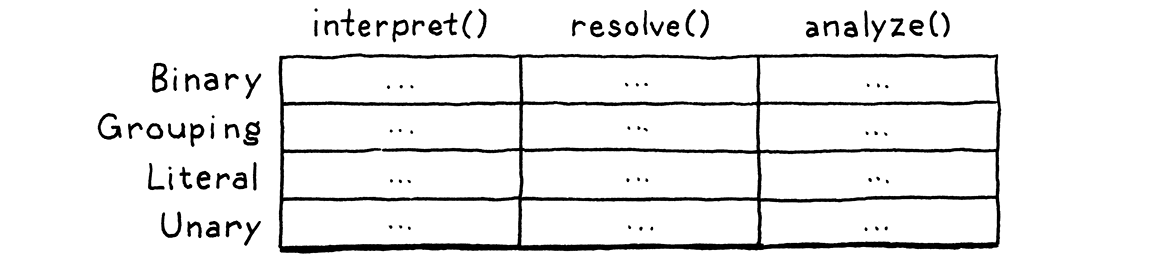
\includegraphics[width=\textwidth]{image/representing-code/table.png}
\end{figure}

行是类型,列是操作。每个单元格表示在该类型上实现该操作的唯一代码段。

像Java这样的面向对象的语言,假定一行中的所有代码都自然地挂在一起。它认为你对一个类型所做的所有事情都可能是相互关联的,而使用这类语言可以很容易将它们一起定义为同一个类里面的方法。

\begin{figure}[htbp]
  \centering
  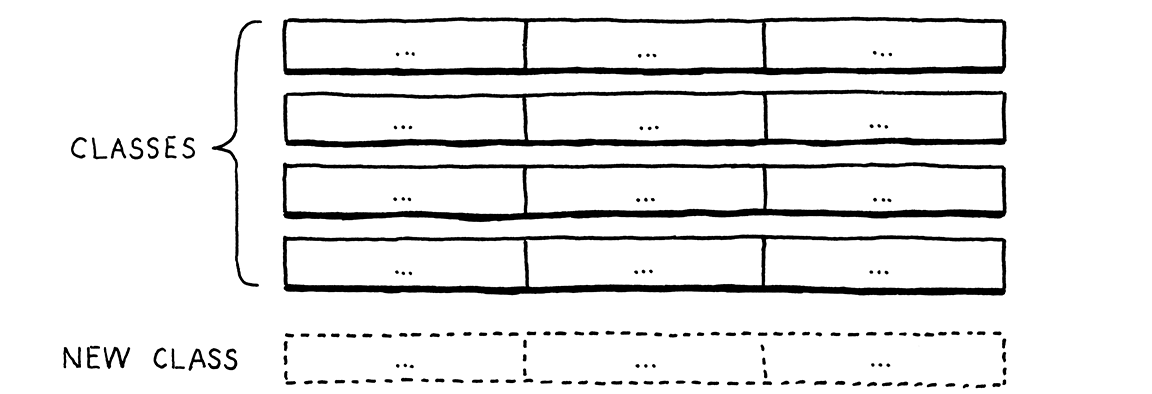
\includegraphics[width=\textwidth]{image/representing-code/rows.png}
\end{figure}

这种情况下,向表中加入新行来扩展列表是很容易的,简单地定义一个新类即可,不需要修改现有的代码。但是,想象一下,如果你要添加一个新操作(新的一行)。在Java中,这意味着要拆开已有的那些类并向其中添加方法。

ML家族中的函数式范型反过来了。在这些语言中,没有带方法的类,类型和函数是完全独立的。要为许多不同类型实现一个操作,只需定义一个函数。在该函数体中,您可以使用\textit{模式匹配}(某种基于类型的switch操作)在同一个函数中实现每个类型对应的操作。

这使得添加新操作非常简单——只需定义另一个与所有类型模式匹配的的函数即可。

\begin{figure}[htbp]
  \centering
  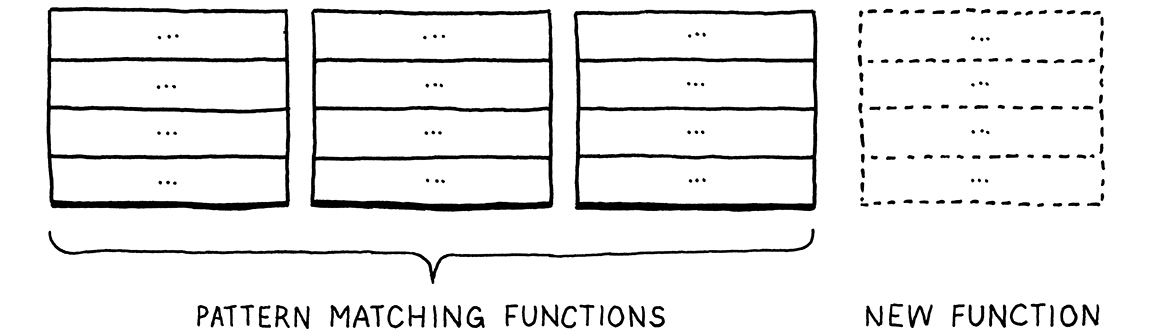
\includegraphics[width=\textwidth]{image/representing-code/columns.png}
\end{figure}

但是,反过来说,添加新类型是困难的。您必须回头向已有函数中的所有模式匹配添加一个新的case。

每种风格都有一定的“纹路”。这就是范式名称的字面意思——面向对象的语言希望你按照类型的行来\textit{组织}你的代码。而函数式语言则鼓励你把每一列的代码都归纳为一个\textit{函数}。

一群聪明的语言迷注意到,这两种风格都不容易向表格中添加行和列。他们称这个困难为“表达式问题”。就像我们现在一样,他们是在试图找出在编译器中建模表达式语法树节点的最佳方法时,第一次遇到了该问题。

人们已经抛出了各种各样的语言特性、设计模式和编程技巧,试图解决这个问题,但还没有一种完美的语言能够解决它。与此同时,我们所能做的就是尽量选择一种与我们正在编写的程序的自然架构相匹配的语言。

面向对象在我们的解释器的许多部分都可以正常工作,但是这些树类与Java的本质背道而驰。幸运的是,我们可以采用一种设计模式来解决这个问题。

\subsection{访问者模式}

\textbf{访问者模式}是所有\textit{设计模式}中最容易被误解的模式,当您回顾过去几十年的软件架构泛滥状况时,会发现确实如此。

问题出在术语上。这个模式不是关于“visiting(访问)”,它的“accept”方法也没有让人产生任何有用的想象。许多人认为这种模式与遍历树有关,但事实并非如此。我们确实要在一组树结构的类上使用它,但这只是一个巧合。如您所见,该模式在单个对象上也可以正常使用。

访问者模式实际上近似于OOP语言中的函数式。它让我们可以很容易地向表中添加新的列。我们可以在一个地方定义针对一组类型的新操作的所有行为,而不必触及类型本身。这与我们解决计算机科学中几乎所有问题的方式相同:添加中间层。

在将其应用到自动生成的Expr类之前,让我们先看一个更简单的例子。比方说我们有两种点心:Beignet(卷饼)和Cruller(油酥卷)。

\begin{code}{java}{}{}
 abstract class Pastry {
  }

  class Beignet extends Pastry {
  }

  class Cruller extends Pastry {
  }
\end{code}

我们希望能够定义新的糕点操作(烹饪,食用,装饰等),而不必每次都向每个类添加新方法。我们是这样做的。首先,我们定义一个单独的接口。

\begin{code}{java}{}{}
  interface PastryVisitor {
    void visitBeignet(Beignet beignet); 
    void visitCruller(Cruller cruller);
  }
\end{code}

可以对糕点执行的每个操作都是实现该接口的新类。它对每种类型的糕点都有具体的方法。这样一来,针对两种类型的操作代码都紧密地嵌套在一个类中。

给定一个糕点,我们如何根据其类型将其路由到访问者的正确方法?多态性拯救了我们!我们在Pastry中添加这个方法:

\begin{code}{java}{}{}
  abstract class Pastry {
    abstract void accept(PastryVisitor visitor);
  }
\end{code}

每个子类都需要实现该方法:

\begin{code}{java}{}{}
  class Beignet extends Pastry {
    @Override
    void accept(PastryVisitor visitor) {
      visitor.visitBeignet(this);
    }
  }
\end{code}

以及:

\begin{code}{java}{}{}
  class Cruller extends Pastry {
    @Override
    void accept(PastryVisitor visitor) {
      visitor.visitCruller(this);
    }
  }
\end{code}

要对糕点执行一个操作,我们就调用它的accept()方法,并将我们要执行的操作vistor作为参数传入该方法。pastry类——特定子类对accept()的重写实现——会反过来,在visitor上调用合适的visit方法,并将\textit{自身}作为参数传入。

这就是这个技巧的核心所在。它让我们可以在\textit{pastry}类上使用多态派遣,在\textit{visitor}类上选择合适的方法。对应在表格中,每个pastry类都是一行,但如果你看一个visitor的所有方法,它们就会形成一\textit{列}。

\begin{figure}[htbp]
  \centering
  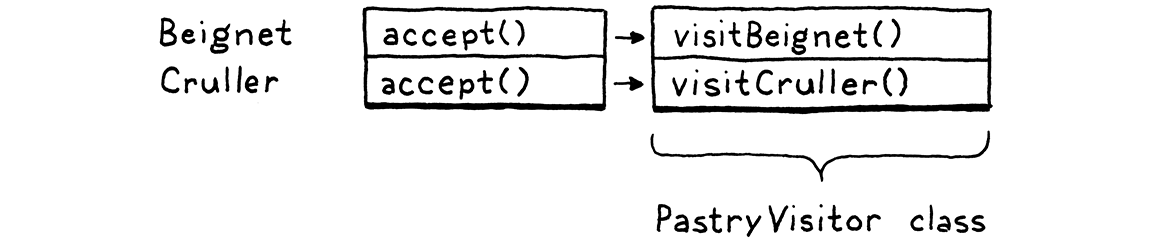
\includegraphics[width=\textwidth]{image/representing-code/visitor.png}
\end{figure}

我们为每个类添加了一个accept()方法,我们可以根据需要将其用于任意数量的访问者,而无需再次修改\textit{pastry}类。这是一个聪明的模式。

\subsection{表达式访问者}

好的,让我们将它编入表达式类中。我们还要对这个模式进行一下完善。在糕点的例子中,visit和accept()方法没有返回任何东西。在实践中,访问者通常希望定义能够产生值的操作。但accept()应该具有什么返回类型呢?我们不能假设每个访问者类都想产生相同的类型,所以我们将使用泛型来让每个实现类自行填充一个返回类型。

首先,我们定义访问者接口。同样,我们把它嵌套在基类中,以便将所有的内容都放在一个文件中。

\begin{code}{java}{2}{tool/GenerateAst.java,在defineAst()方法中添加}
    writer.println("abstract class " + baseName + " {");
    defineVisitor(writer, baseName, types);
    // The AST classes.
\end{code}

这个函数会生成visitor接口。

\begin{code}{java}{}{tool/GenerateAst.java,在defineAst()方法后添加}
  private static void defineVisitor(
      PrintWriter writer, String baseName, List<String> types) {
    writer.println("  interface Visitor<R> {");

    for (String type : types) {
      String typeName = type.split(":")[0].trim();
      writer.println("    R visit" + typeName + baseName + "(" +
          typeName + " " + baseName.toLowerCase() + ");");
    }

    writer.println("  }");
  }
\end{code}

在这里,我们遍历所有的子类,并为每个子类声明一个visit方法。当我们以后定义新的表达式类型时,会自动包含这些内容。

在基类中,定义抽象accept()方法。

\begin{code}{java}{3-5}{tool/GenerateAst.java,在defineAst()方法中添加}
      defineType(writer, baseName, className, fields);
    }
    // The base accept() method.
    writer.println();
    writer.println("  abstract <R> R accept(Visitor<R> visitor);");
    writer.println("}");
\end{code}

最后,每个子类都实现该方法,并调用其类型对应的visit方法。

\begin{code}{java}{2-8}{tool/GenerateAst.java,在defineType()方法中添加}
    writer.println("    }");
    // Visitor pattern.
    writer.println();
    writer.println("    @Override");
    writer.println("    <R> R accept(Visitor<R> visitor) {");
    writer.println("      return visitor.visit" +
        className + baseName + "(this);");
    writer.println("    }");
    // Fields.
\end{code}

这下好了。现在我们可以在表达式上定义操作,而且无需对类或生成器脚本进行修改。编译并运行这个生成器脚本,输出一个更新后的“Expr.java”文件。该文件中包含一个生成的Visitor接口和一组使用该接口支持Visitor模式的表达式节点类。

在结束这一章的闲聊之前,我们先实现一下这个Visitor接口,看看这个模式的运行情况。

\section{一个(不是很)漂亮的打印器}

当我们调试解析器和解释器时,查看解析后的语法树并确保其与期望的结构一致通常是很有用的。我们可以在调试器中进行检查,但那可能有点难。

相反,我们需要一些代码,在给定语法树的情况下,生成一个明确的字符串表示。将语法树转换为字符串是解析器的逆向操作,当我们的目标是产生一个在源语言中语法有效的文本字符串时,通常被称为“漂亮打印”。

这不是我们的目标。我们希望字符串非常明确地显示树的嵌套结构。如果我们要调试的是操作符的优先级是否处理正确,那么返回1 + 2 * 3的打印器并没有什么用,我们想知道+或*是否在语法树的顶部。

因此,我们生成的字符串表示形式不是Lox语法。相反,它看起来很像Lisp。每个表达式都被显式地括起来,并且它的所有子表达式和词法标记都包含在其中。

给定一个语法树,如:

\begin{figure}[htbp]
  \centering
  
\includegraphics[width=\textwidth]{image/representing-code/expression.png}
\end{figure}

输出结果为:

\begin{code}{js}{}{}
(* (- 123) (group 45.67))
\end{code}

不是很“漂亮”,但是它确实明确地展示了嵌套和分组。为了实现这一点,我们定义了一个新类。

\begin{code}{java}{}{lox/AstPrinter.java,创建新文件}
package com.craftinginterpreters.lox;

class AstPrinter implements Expr.Visitor<String> {
  String print(Expr expr) {
    return expr.accept(this);
  }
}
\end{code}

如你所见,它实现了visitor接口。这意味着我们需要为我们目前拥有的每一种表达式类型提供visit方法。

\begin{code}{java}{4-24}{lox/AstPrinter.java,在print()方法后添加}
  return expr.accept(this);
  }

  @Override
  public String visitBinaryExpr(Expr.Binary expr) {
    return parenthesize(expr.operator.lexeme,
                        expr.left, expr.right);
  }

  @Override
  public String visitGroupingExpr(Expr.Grouping expr) {
    return parenthesize("group", expr.expression);
  }

  @Override
  public String visitLiteralExpr(Expr.Literal expr) {
    if (expr.value == null) return "nil";
    return expr.value.toString();
  }

  @Override
  public String visitUnaryExpr(Expr.Unary expr) {
    return parenthesize(expr.operator.lexeme, expr.right);
  }
}
\end{code}

字面量表达式很简单——它们将值转换为一个字符串,并通过一个小检查用Java中的null代替Lox中的nil。其他表达式有子表达式,所以它们要使用parenthesize()这个辅助方法:

\begin{code}{java}{}{lox/AstPrinter.java,在visitUnaryExpr()方法后添加}
  private String parenthesize(String name, Expr... exprs) {
    StringBuilder builder = new StringBuilder();

    builder.append("(").append(name);
    for (Expr expr : exprs) {
      builder.append(" ");
      builder.append(expr.accept(this));
    }
    builder.append(")");

    return builder.toString();
  }
\end{code}

它接收一个名称和一组子表达式作为参数,将它们全部包装在圆括号中,并生成一个如下的字符串:

\begin{code}{js}{}{}
(+ 1 2)
\end{code}

请注意,它在每个子表达式上调用accept()并将自身传递进去。这是递归步骤,可让我们打印整棵树。

我们还没有解析器,所以很难看到它的实际应用。现在,我们先使用一个main()方法来手动实例化一个树并打印它。

\begin{code}{java}{}{lox/AstPrinter.java,在parenthesize()方法后添加}
  public static void main(String[] args) {
    Expr expression = new Expr.Binary(
        new Expr.Unary(
            new Token(TokenType.MINUS, "-", null, 1),
            new Expr.Literal(123)),
        new Token(TokenType.STAR, "*", null, 1),
        new Expr.Grouping(
            new Expr.Literal(45.67)));

    System.out.println(new AstPrinter().print(expression));
  }
\end{code}

如果我们都做对了,它就会打印:

\begin{code}{js}{}{}
(* (- 123) (group 45.67))
\end{code}

您可以继续删除这个方法,我们后面不再需要它了。另外,当我们添加新的语法树类型时,我不会在AstPrinter中展示它们对应的visit方法。如果你想这样做(并且希望Java编译器不会报错),那么你可以自行添加这些方法。在下一章,当我们开始将Lox代码解析为语法树时,它将会派上用场。或者,如果你不想维护AstPrinter,可以随意删除它。我们不再需要它了。

\section{挑战}

\begin{enumerate}
  \item 之前我说过,我们在语法元语法中添加的|、*、+等形式只是语法糖。以这个语法为例:

\begin{ebnf}
expr & \rightarrow \quad expr \quad ( \quad \mathtt{"}(\mathtt{"} \quad ( \quad expr \quad ( \quad \mathtt{"},\mathtt{"} \quad expr \quad )* \quad )? \quad \mathtt{"})\mathtt{"} \\
     & \;\;\vert \quad \mathtt{"}.\mathtt{"} \quad IDENTIFIER \quad )+ \\
     & \;\;\vert\quad IDENTIFIER \\
     & \;\;\vert\quad NUMBER
\end{ebnf}

生成一个与同一语言相匹配的语法,但不要使用任何语法糖。

附加题:这一点语法表示了什么样的表达式?

  \item Visitor模式让你可以在面向对象的语言中模仿函数式。为函数式语言设计一个互补的模式,该模式让你可以将一个类型上的所有操作捆绑在一起,并轻松扩展新的类型。

(SML或Haskell是这个练习的理想选择,但Scheme或其它Lisp方言也可以。)

  \item 在逆波兰表达式(RPN)中,算术运算符的操作数都放在运算符之前,所以1 + 2变成了1 2 +。计算时从左到右进行,操作数被压入隐式栈。算术运算符弹出前两个数字,执行运算,并将结果推入栈中。因此,

\begin{code}{java}{}{}
(1 + 2) * (4 - 3)
\end{code}

在RPN中变为了

\begin{code}{js}{}{}
1 2 + 4 3 - *
\end{code}

为我们的语法树类定义一个Vistor类,该类接受一个表达式,将其转换为RPN,并返回结果字符串。
\end{enumerate}

\chapter{解析表达式}

\epigraph{语法,它甚至知道如何控制国王。}{莫里哀}

本章是本书的第一个重要里程碑。我们中的许多人都曾将正则表达式和字符串操作的糅合在一起,以便从一堆文本中提取一些信息。这些代码可能充满了错误,而且很难维护。编写一个真正的解析器——具有良好的错误处理、一致的内部结构和能够健壮地分析复杂语法的能力——被认为是一种罕见的、令人印象深刻的技能。在这一章中,你将获得这种技能。

这比想象中要简单,部分是因为我们在上一章中提前完成了很多困难的工作。你已经对形式化语法了如指掌,也熟悉了语法树,而且我们有一些Java类来表示它们。唯一剩下的部分是解析——将一个标记序列转换成这些语法树中的一个。

一些CS教科书在解析器上大做文章。在60年代,计算机科学家——他们理所当然地厌倦了用汇编语言编程——开始设计更复杂的、对人类友好的语言,比如Fortran和ALGOL。唉,对于当时原始的计算机来说,这些语言对机器并不友好。

这些先驱们设计了一些语言,说实话,他们甚至不知道如何编写编译器。然后他们做了开创性的工作,发明了解析和编译技术,可以在那些老旧、小型的机器上处理这些新的、大型的语言。

经典的编译书读起来就像是对这些英雄和他们的工具的吹捧传记。《编译器:原理、技术和工具》的封面上有一条标记着“编译器设计复杂性”的龙,被一个手持剑和盾的骑士杀死,剑和盾上标记着“LALR解析器生成器”和“语法制导翻译”。他们在过分吹捧。

稍微的自我祝贺是当之无愧的,但事实是,你不需要知道其中的大部分知识,就可以为现代机器制作出高质量的解析器。一如既往,我鼓励你先扩大学习范围,以后再慢慢接受它,但这本书省略了奖杯箱。

\section{歧义与解析游戏}

在上一章中,我说过你可以像“玩”游戏一样使用上下文无关的语法来\textit{生成}字符串。解析器则以相反的方式玩游戏。给定一个字符串(一系列语法标记),我们将这些标记映射到语法中的终止符,以确定哪些规则可能生成该字符串。

“可能产生”这部分很有意思。我们完全有可能创建一个\textit{模棱两可}的语法,在这个语法中,不同的生成式可能会得到同一个字符串。当你使用该语法来\textit{生成}字符串时,这一点不太重要。一旦你有了字符串,谁还会在乎你是怎么得到它的呢?

但是在解析时,歧义意味着解析器可能会误解用户的代码。当我们进行解析时,我们不仅要确定字符串是不是有效的Lox代码,还要记录哪些规则与代码的哪些部分相匹配,以便我们知道每个标记属于语言的哪一部分。下面是我们在上一章整理的Lox表达式语法:

\begin{ebnf}
expression & \rightarrow \quad literal \\
           & \;\;\vert \quad unary \\
           & \;\;\vert \quad binary \\
           & \;\;\vert \quad grouping \quad ; \\
\\
literal   & \rightarrow \quad NUMBER \quad\vert\quad STRING \quad\vert\quad \mathtt{"}true\mathtt{"} \quad\vert\quad \mathtt{"}false\mathtt{"} \quad\vert\quad \mathtt{"}nil\mathtt{"} \quad ; \\
grouping  & \rightarrow \quad \mathtt{"}(\mathtt{"} \quad expression \mathtt{"})\mathtt{"} \quad ; \\
unary     & \rightarrow \quad ( \quad \mathtt{"}-\mathtt{"} \quad\vert\quad \mathtt{"}!\mathtt{"} \quad ) \quad expression \quad ; \\
binary    & \rightarrow \quad expression \quad operator \quad expression \quad ; \\
operator  & \rightarrow \quad \mathtt{"}==\mathtt{"} \quad\vert\quad \mathtt{"}!=\mathtt{"} \quad\vert\quad \mathtt{"}<\mathtt{"} \quad\vert\quad \mathtt{"}<=\mathtt{"} \quad\vert\quad \mathtt{"}>\mathtt{"} \quad\vert\quad \mathtt{"}>=\mathtt{"} \\
& \;\;\vert\quad \mathtt{"}+\mathtt{"} \quad\vert\quad \mathtt{"}-\mathtt{"} \quad\vert\quad \mathtt{"}*\mathtt{"} \quad\vert\quad \mathtt{"}/\mathtt{"} \quad ;
\end{ebnf}

下面是一个满足语法的有效字符串:

\begin{figure}[htbp]
  \centering
  
\includegraphics[width=\textwidth]{image/parsing-expressions/tokens.png}
\end{figure}

但是,有两种方式可以生成该字符串。其一是:

\begin{enumerate}
  \item 从expression开始,选择binary。
  \item 对于左边的expression,选择NUMBER,并且使用6。
  \item 对于操作符,选择/。
  \item 对于右边的expression,再次选择binary。
  \item 在内层的binary表达式中,选择3-1。
\end{enumerate}

其二是:

\begin{enumerate}
  \item 从expression开始,选择binary。
  \item 对于左边的expression,再次选择binary。
  \item 在内层的binary表达式中,选择6/3。
  \item 返回外层的binary,对于操作符,选择-。
  \item 对于右边的expression,选择NUMBER,并且使用1。
\end{enumerate}

它们产生相同的字符串,但对应的是不同的\textit{语法树}:

\begin{figure}[htbp]
  \centering
  
\includegraphics[width=\textwidth]{image/parsing-expressions/syntax-trees.png}
\end{figure}

换句话说,这个语法可以将该表达式看作是(6 / 3) - 1或6 / (3 - 1)。binary规则运行操作数以任意方式嵌套,这反过来又会影响解析数的计算结果。自从黑板被发明以来,数学家们解决这种模糊性的方法就是定义优先级和结合性规则。

\begin{itemize}
  \item \textbf{优先级}决定了在一个包含不同运算符的混合表达式中,哪个运算符先被执行。优先级规则告诉我们,在上面的例子中,我们在-之前先计算/。优先级较高的运算符在优先级较低的运算符之前计算。同样,优先级较高的运算符被称为“更严格的绑定”。
  \item \textbf{结合性}决定在一系列相同操作符中先计算哪个操作符。如果一个操作符是\textbf{左结合}的(可以认为是“从左到右”)时,左边的操作符在右边的操作符之前计算。因为-是左结合的,下面的表达式:

  \begin{code}{java}{}{}
  5 - 3 - 1
  \end{code}

  等价于:

  \begin{code}{java}{}{}
  (5 - 3) - 1
  \end{code}

  另一方面,赋值是\textbf{右结合}的。如:

  \begin{code}{java}{}{}
  a = b = c
  \end{code}

  等价于:

  \begin{code}{java}{}{}
  a = (b = c)
  \end{code}
\end{itemize}

如果没有明确定义的优先级和结合性,使用多个运算符的表达式可能就会变得有歧义——它可以被解析为不同的语法树,而这些语法树又可能会计算出不同的结果。我们在Lox中会解决这个问题,使用与C语言相同的优先级规则,从低到高分别是:

\begin{center}
  \begin{tabular}{ |c|c|c| }
   \hline
   名字 & 运算符 & 结合性 \\
   \hline
   等于 & ==,!= & 左结合 \\ 
   比较 & >,>=,<,<= & 左结合 \\
   加减 & +,- & 左结合 \\
   乘除 & /,* & 左结合 \\
   一元 & !,- & 右结合 \\ 
   \hline
  \end{tabular}
\end{center}

现在,该语法将所有表达式类型都添加到一个expression规则中。这条规则同样作用于操作数中的非终止符,这使得语法中可以接受任何类型的表达式作为子表达式,而不管优先级规则是否允许。

我们通过对语法进行分层来解决这个问题。我们为每个优先级定义一个单独的规则。

\begin{ebnf}
expression & \rightarrow \quad ... \\
equality   & \rightarrow \quad ... \\
comparison & \rightarrow \quad ... \\
term       & \rightarrow \quad ... \\
factor     & \rightarrow \quad ... \\
unary      & \rightarrow \quad ... \\
primary    & \rightarrow \quad ...
\end{ebnf}

此处的每个规则仅匹配其当前优先级或更高优先级的表达式。 例如,unary匹配一元表达式(如 !negated)或主表达式(如1234)。term可以匹配1 + 2,但也可以匹配3 * 4 /5。最后的primary规则涵盖优先级最高的形式——字面量和括号表达式。

我们只需要填写每条规则的生成式。我们先从简单的开始。顶级的expression规则可以匹配任何优先级的表达式。由于equality的优先级最低,只要我们匹配了它,就涵盖了一切。

\begin{ebnf}
expression \rightarrow\quad equality
\end{ebnf}

在优先级表的另一端,primary表达式包括所有的字面量和分组表达式。

\begin{ebnf}
primary & \rightarrow \quad NUMBER \quad\vert\quad STRING \quad\vert\quad \mathtt{"}true\mathtt{"} \quad\vert\quad \mathtt{"}false\mathtt{"} \quad\vert\quad \mathtt{"}nil\mathtt{"} \\
        & \;\;\vert\quad \mathtt{"}(\mathtt{"} expression \mathtt{"})\mathtt{"} \quad ;
\end{ebnf}

一元表达式以一元操作符开头,后跟操作数。因为一元操作符可以嵌套——!!true虽奇怪也是可用的表达式——这个操作数本身可以是一个一元表达式。递归规则可以很好地解决这个问题。

\begin{ebnf}
unary \rightarrow \quad ( \quad \mathtt{"}!\mathtt{"} \quad\vert\quad \mathtt{"}-\mathtt{"} \quad ) \quad unary \quad ;
\end{ebnf}

但是这条规则有一个问题,它永远不会终止。

请记住,每个规则都需要匹配该优先级或更高优先级的表达式,因此我们还需要使其与主表达式匹配。

\begin{ebnf}
unary & \rightarrow \quad ( \quad \mathtt{"}!\mathtt{"} \quad\vert\quad \mathtt{"}-\mathtt{"} \quad ) \quad unary \\
      & \;\;\vert \quad primary \quad ;
\end{ebnf}

这样就可以了。

剩下的规则就是二元运算符。我们先从乘法和除法的规则开始。下面是第一次尝试:

\begin{ebnf}
factor & \rightarrow \quad factor \quad ( \quad \mathtt{"}/\mathtt{"} \quad\vert\quad \mathtt{"}*\mathtt{"} \quad ) \quad unary \\
       & \;\;\vert\quad unary \quad ;
\end{ebnf}

该规则递归匹配左操作数,这样一来,就可以匹配一系列乘法和除法表达式,例如1 * 2 / 3。将递归生成式放在左侧并将unary放在右侧,可以使该规则具有左关联性和明确性。

所有这些都是正确的,但规则主体中的第一个符号与规则头部相同意味着这个生成式是\textbf{左递归}的。一些解析技术,包括我们将要使用的解析技术,在处理左递归时会遇到问题。(其他地方的递归,比如在unary中,以及在primary分组中的间接递归都不是问题。)

你可以定义很多符合同一种语言的语法。如何对某一特定语言进行建模,一部分是品味问题,一部分是实用主义问题。这个规则是正确的,但对于我们后续的解析来说它并不是最优的。我们将使用不同的规则来代替左递归规则。

\begin{ebnf}
factor \rightarrow\quad unary \quad ( \quad ( \quad \mathtt{"}/\mathtt{"} \quad\vert\quad \mathtt{"}*\mathtt{"} \quad ) \quad unary \quad )* \quad ;
\end{ebnf}

我们将因子表达式定义为乘法和除法的扁平\textit{序列}。这与前面的规则语法相同,但更好地反映了我们将编写的解析Lox的代码。我们对其它二进制运算符的优先级使用相同的结构,从而得到下面这个完整的表达式语法:

\begin{ebnf}
\footnotesize
expression     & \rightarrow\quad equality \quad ; \\
equality       & \rightarrow\quad comparison \quad ( \quad ( \quad \mathtt{"}!=\mathtt{"} \quad\vert\quad \mathtt{"}==\mathtt{"} \quad ) \quad comparison \quad )* \quad ; \\
comparison     & \rightarrow\quad term \quad ( \quad ( \quad \mathtt{"}>\mathtt{"} \quad\vert\quad \mathtt{"}>=\mathtt{"} \quad\vert\quad \mathtt{"}<\mathtt{"} \\
               & \;\;\vert\quad \mathtt{"}<=\mathtt{"} \quad ) \quad term \quad )* \quad ; \\
term           & \rightarrow\quad factor \quad ( \quad ( \quad \mathtt{"}-\mathtt{"} \quad\vert\quad \mathtt{"}+\mathtt{"} \quad ) \quad factor \quad )* \quad ; \\
factor         & \rightarrow\quad unary \quad ( \quad ( \quad \mathtt{"}/\mathtt{"} \quad\vert\quad \mathtt{"}*\mathtt{"} \quad ) \quad unary \quad )* \quad ; \\
unary          & \rightarrow\quad ( \quad \mathtt{"}!\mathtt{"} \quad\vert\quad \mathtt{"}-\mathtt{"} \quad ) \quad unary \\
               & \;\;\vert\quad primary \quad ; \\
primary        & \rightarrow\quad NUMBER \quad\vert\quad STRING \quad\vert\quad \mathtt{"}true\mathtt{"} \quad\vert\quad \mathtt{"}false\mathtt{"} \quad\vert\quad \mathtt{"}nil\mathtt{"} \\
               & \;\;\vert\quad \mathtt{"}(\mathtt{"} \quad expression \quad \mathtt{"})\mathtt{"} \quad ;
\end{ebnf}

这个语法比我们以前的那个更复杂,但反过来我们也消除了前一个语法定义中的歧义。这正是我们制作解析器时所需要的。

\section{递归下降分析}

现在有一大堆解析技术,它们的名字大多是“L”和“R”的组合——LL(k)、LR(1)、LALR——还有更多的异类,比如解析器组合子、Earley parsers、分流码算法和packrat解析。对于我们的第一个解释器来说,一种技术已经足够了:\textbf{递归下降}。

递归下降是构建解析器最简单的方法,不需要使用复杂的解析器生成工具,如Yacc、Bison或ANTLR。你只需要直接手写代码。但是不要被它的简单性所欺骗,递归下降解析器速度快、健壮,并且可以支持复杂的错误处理。事实上,GCC、V8 (Chrome中的JavaScript VM)、Roslyn(用C\#编写的C\#编译器)和许多其他重量级产品语言实现都使用了递归下降技术。它很好用。

递归下降被认为是一种\textbf{自顶向下解析器},因为它从最顶部或最外层的语法规则(这里是expression)开始,一直向下进入嵌套子表达式,最后到达语法树的叶子。这与LR等自下而上的解析器形成鲜明对比,后者从初级表达式(primary)开始,将其组成越来越大的语法块。

递归下降解析器是一种将语法规则直接翻译成命令式代码的文本翻译器。每个规则都会变成一个函数,规则主体翻译成代码大致是这样的:

\begin{center}
  \begin{tabular}{ |c|c| } 
   \hline
   语法记号 & 代码表示 \\
   \hline 
   终结符 & 匹配并消费一个词法标记 \\ 
   非终结符 & 调用规则对应的函数 \\
   | & if或者switch语句 \\
   *或者+ & while或者for循环 \\
   ? & if语句 \\ 
   \hline
  \end{tabular}
\end{center}

下降被“递归”修饰是因为,如果一个规则引用自身(直接或间接)就会变为递归的函数调用。

\subsection{Parser类}

每个语法规则都成为新类中的一个方法:

\begin{code}{java}{}{lox/Parser.java,创建新文件}
package com.craftinginterpreters.lox;

import java.util.List;

import static com.craftinginterpreters.lox.TokenType.*;

class Parser {
  private final List<Token> tokens;
  private int current = 0;

  Parser(List<Token> tokens) {
    this.tokens = tokens;
  }
}
\end{code}

与扫描器一样,解析器也是消费一个扁平的输入序列,这是这次我们要读取的是语法标记而不是字符。我们会保存标记列表并使用current指向待解析的下一个标记。

我们现在要直接执行表达式语法,并将每一条规则翻译为Java代码。第一条规则expression,简单地展开为equality规则,所以很直接:

\begin{code}{java}{}{lox/Parser.java,在Parser()方法添加}
  private Expr expression() {
    return equality();
  }
\end{code}

每个解析语法规则的方法都会生成该规则对应的语法树,并将其返回给调用者。当规则主体中包含一个非终止符——对另一条规则的引用时,我们就会调用另一条规则对应的方法。

等式规则有一点复杂:

\begin{ebnf}
equality \rightarrow \quad comparison \quad ( \quad ( \quad \mathtt{"}!=\mathtt{"} \quad\vert\quad \mathtt{"}==\mathtt{"} \quad ) \quad comparison \quad )* \quad ;
\end{ebnf}

在Java中,这会变成:

\begin{code}{java}{}{lox/Parser.java,在expression()后面添加}
  private Expr equality() {
    Expr expr = comparison();

    while (match(BANG_EQUAL, EQUAL_EQUAL)) {
      Token operator = previous();
      Expr right = comparison();
      expr = new Expr.Binary(expr, operator, right);
    }

    return expr;
  }
\end{code}

让我们一步步来。规则体中的第一个comparison非终止符变成了方法中对comparison()的第一次调用。我们获取结果并将其保存在一个局部变量中。

然后,规则中的(...)*循环映射为一个while循环。我们需要知道何时退出这个循环。可以看到,在规则体中,我们必须先找到一个!=或==标记。因此,如果我们\textit{没有}看到其中任一标记,我们必须结束相等(不相等)运算符的序列。我们使用一个方便的match()方法来执行这个检查。

\begin{code}{java}{}{lox/Parser.java,在equality()方法后添加}
  private boolean match(TokenType... types) {
    for (TokenType type : types) {
      if (check(type)) {
        advance();
        return true;
      }
    }

    return false;
  }
\end{code}

这个检查会判断当前的标记是否属于给定的类型之一。如果是,则消费该标记并返回true;否则,就返回false并保留当前标记。match()方法是由两个更基本的操作来定义的。

如果当前标记属于给定类型,则check()方法返回true。与match()不同的是,它从不消费标记,只是读取。

\begin{code}{java}{}{lox/Parser.java,在match()方法后添加}
  private boolean check(TokenType type) {
    if (isAtEnd()) return false;
    return peek().type == type;
  }
\end{code}

advance()方法会消费当前的标记并返回它,类似于扫描器中对应方法处理字符的方式。

\begin{code}{java}{}{lox/Parser.java,在check()方法后添加}
  private Token advance() {
    if (!isAtEnd()) current++;
    return previous();
  }
\end{code}

这些方法最后都归结于几个基本操作。

\begin{code}{java}{}{lox/Parser.java,在advance()后添加}
  private boolean isAtEnd() {
    return peek().type == EOF;
  }

  private Token peek() {
    return tokens.get(current);
  }

  private Token previous() {
    return tokens.get(current - 1);
  }
\end{code}

isAtEnd()检查我们是否处理完了待解析的标记。peek()方法返回我们还未消费的当前标记,而previous()会返回最近消费的标记。后者让我们更容易使用match(),然后访问刚刚匹配的标记。

这就是我们需要的大部分解析基本工具。我们说到哪里了?对,如果我们在equality()的while循环中,也就能知道我们已经找到了一个!=或==操作符,并且一定是在解析一个等式表达式。

我们获取到匹配的操作符标记,这样就可以知道我们要处理哪一类等式表达式。之后,我们再次调用comparison()解析右边的操作数。我们将操作符和它的两个操作数组合成一个新的Expr.Binary语法树节点,然后开始循环。对于每一次迭代,我们都将结果表达式存储在同一个expr局部变量中。在对等式表达式序列进行压缩时,会创建一个由二元操作符节点组成的左结合嵌套树。

\begin{figure}[htbp]
  \centering
  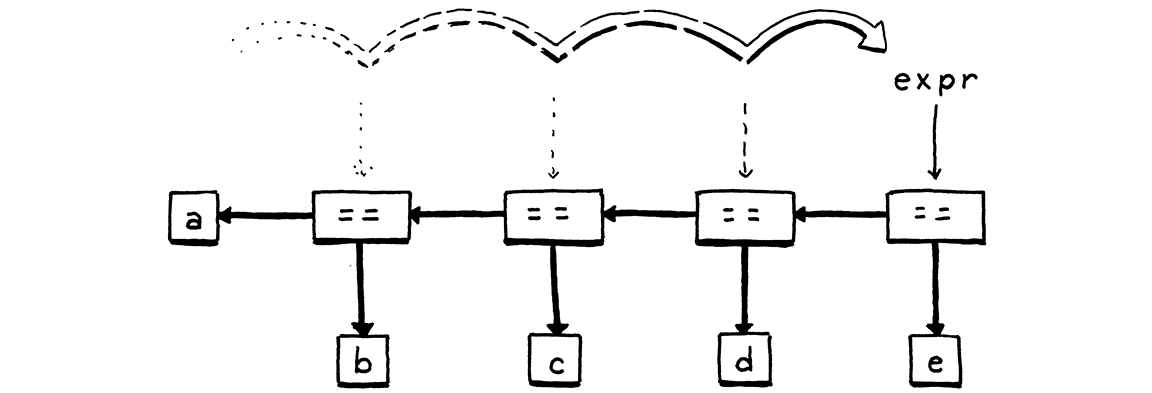
\includegraphics[width=\textwidth]{image/parsing-expressions/sequence.png}
\end{figure}

一旦解析器遇到一个不是等式操作符的标记,就会退出循环。最后,它会返回对应的表达式。请注意,如果解析器从未遇到过等式操作符,它就永远不会进入循环。在这种情况下,equality()方法有效地调用并返回comparison()。这样一来,这个方法就会匹配一个等式运算符或\textit{任何更高优先级的表达式}。

继续看下一个规则。

\begin{ebnf}
comparison & \rightarrow\quad term \quad ( \quad ( \quad \mathtt{"}>\mathtt{"} \quad\vert\quad \mathtt{"}>=\mathtt{"} \\
& \;\;\vert\quad \mathtt{"}<\mathtt{"} \quad\vert\quad \mathtt{"}<=\mathtt{"} \quad ) \quad term \quad )* \quad ;
\end{ebnf}

翻译成Java:

\begin{code}{java}{}{lox/Parser.java,在equality()方法后添加}
  private Expr comparison() {
    Expr expr = term();

    while (match(GREATER, GREATER_EQUAL, LESS, LESS_EQUAL)) {
      Token operator = previous();
      Expr right = term();
      expr = new Expr.Binary(expr, operator, right);
    }

    return expr;
  }
\end{code}

语法规则与equality几乎完全相同,相应的代码也是如此。唯一的区别是匹配的操作符的标记类型,而且现在获取操作数时调用的方法是term()而不是comparison()。其余两个二元操作符规则遵循相同的模式。

按照优先级顺序,先做加减法:

\begin{code}{java}{}{lox/Parser.java,在comparison()方法后添加}
  private Expr term() {
    Expr expr = factor();

    while (match(MINUS, PLUS)) {
      Token operator = previous();
      Expr right = factor();
      expr = new Expr.Binary(expr, operator, right);
    }

    return expr;
  }
\end{code}

最后,是乘除法:

\begin{code}{java}{}{lox/Parser.java,在term()方法后面添加}
  private Expr factor() {
    Expr expr = unary();

    while (match(SLASH, STAR)) {
      Token operator = previous();
      Expr right = unary();
      expr = new Expr.Binary(expr, operator, right);
    }

    return expr;
  }
\end{code}

这就是所有的二进制运算符,已经按照正确的优先级和结合性进行了解析。接下来,按照优先级层级,我们要处理一元运算符了。

\begin{ebnf}
unary & \rightarrow\quad ( \quad \mathtt{"}!\mathtt{"} \quad\vert\quad \mathtt{"}-\mathtt{"} \quad ) \quad unary \\
      & \;\;\vert\quad primary ;
\end{ebnf}

该规则对应的代码有些不同。

\begin{code}{java}{}{lox/Parser.java,在factor()方法后添加}
  private Expr unary() {
    if (match(BANG, MINUS)) {
      Token operator = previous();
      Expr right = unary();
      return new Expr.Unary(operator, right);
    }

    return primary();
  }
\end{code}

同样的,我们先检查当前的标记以确认要如何进行解析。如果是!或-,我们一定有一个一元表达式。在这种情况下,我们获取标记,然后递归调用unary()来解析操作数。将所有这些都包装到一元表达式语法树中,我们就完成了。

否则,我们就达到了最高级别的优先级,即基本表达式。

\begin{ebnf}
  primary & \rightarrow\quad NUMBER \quad\vert\quad STRING \quad\vert\quad \mathtt{"}true\mathtt{"} \\
  & \;\;\vert\quad \mathtt{"}false\mathtt{"} \quad\vert\quad \mathtt{"}nil\mathtt{"} \\
  & \;\;\vert\quad \mathtt{"}(\mathtt{"} expression \mathtt{"})\mathtt{"} ;
\end{ebnf}

该规则中大部分都是终止符,可以直接进行解析。

\begin{code}{java}{}{lox/Parser.java,在unary()方法后添加}
  private Expr primary() {
    if (match(FALSE)) return new Expr.Literal(false);
    if (match(TRUE)) return new Expr.Literal(true);
    if (match(NIL)) return new Expr.Literal(null);

    if (match(NUMBER, STRING)) {
      return new Expr.Literal(previous().literal);
    }

    if (match(LEFT_PAREN)) {
      Expr expr = expression();
      consume(RIGHT_PAREN, "Expect ')' after expression.");
      return new Expr.Grouping(expr);
    }
  }
\end{code}

有趣的一点是处理括号的分支。当我们匹配了一个开头(并解析了里面的表达式后,我们必须找到一个)标记。如果没有找到,那就是一个错误。

\section{语法错误}

解析器实际上有两项工作:

\begin{enumerate}
  \item 给定一个有效的标记序列,生成相应的语法树。
  \item 给定一个\textit{无效}的标记序列,检测错误并告知用户。
\end{enumerate}

不要低估第二项工作的重要性!在现代的IDE和编辑器中,为了语法高亮显示和支持自动补齐等功能,当用户还在编辑代码时,解析器就会不断地重新解析代码。这也意味着解析器\textit{总是}会遇到不完整的、半错误状态的代码。

当用户没有意识到语法错误时,解析器要帮助引导他们回到正确的道路上。它报告错误的方式是你的语言的用户界面中很大的一部分。良好的语法错误处理是很难的。根据定义,代码并不是处于良好定义的状态,所以没有可靠的方法能够知道用户\textit{想要}写什么。解析器无法读懂你的思想。

当解析器遇到语法错误时,有几个硬性要求。解析器必须能够:

\begin{itemize}
  \item \textbf{检测并报告错误。}如果它没有检测到错误,并将由此产生的畸形语法树传递给解释器,就会出现各种可怕的情况。
  \item \textbf{避免崩溃或挂起。}语法错误是生活中不可避免的事实,面对语法错误,语言工具必须非常健壮。段错误或陷入无限循环是不允许的。虽然源代码可能不是有效的\textit{代码},但它仍然是\textit{解析器的有效输入},因为用户使用解析器来了解什么是允许的语法。
\end{itemize}

如果你想参与到解析器的游戏中来,这些就是桌面的筹码,但你真的想提高赌注,除了这些。一个像样的解析器还应该:

\begin{itemize}
  \item \textbf{要快}。计算机的速度比最初发明解析器技术时快了几千倍。那种需要优化解析器,以便它能在喝咖啡的时候处理完整个源文件的日子已经一去不复返了。但是程序员的期望值也上升得同样快,甚至更快。他们希望他们的编辑器能在每次击键后的几毫秒内回复文件。
  \item \textbf{尽可能多地报告出不同的错误}。在第一个错误后中止是很容易实现的,但是如果每次当用户修复文件中的一个错误时,又出现了另一个新的错误,这对用户来说是很烦人的。他们希望一次看到所有的错误。
  \item \textbf{最小化\textit{级联}错误}。一旦发现一个错误,解析器就不再能知道发生了什么。它会试图让自己回到正轨并继续工作,但如果它感到混乱,它可能会报告大量的幽灵错误,而这些错误并不表明代码中存在其它问题。当第一个错误被修正后,这些幽灵错误就消失了,因为它们只反映了解析器自身的混乱。级联错误很烦人,因为它们会让用户害怕,让用户认为自己的代码比实际情况更糟糕。
\end{itemize}

最后两点是相互矛盾的。我们希望尽可能多地报告单独的错误,但我们不想报告那些只是由早期错误的副作用导致的错误。

解析器对一个错误做出反应,并继续去寻找后面的错误的方式叫做\textbf{错误恢复}。这在60年代是一个热门的研究课题。那时,你需要把一叠穿孔卡片交给秘书,第二天再来看看编译器是否成功。在迭代循环如此缓慢的情况下,你真的会想在一次传递中找到代码中的每个错误。

如今,解析器在您甚至还没有完成输入之前就完成解析了,这不再是一个问题。简单,快速的错误恢复就可以了。

\subsection{恐慌模式错误恢复}

在过去设计的所有恢复技术中,最能经受住时间考验的一种叫做\textbf{恐慌模式}(有点令人震惊)。一旦解析器检测到一个错误,它就会进入恐慌模式。它知道至少有一个token是没有意义的,因为它目前的状态是在一些语法生成式的堆栈中间。

在程序继续进行解析之前,它需要将自己的状态和即将到来的标记序列对齐,使下一个标记能够匹配正则解析的规则。这个过程称为\textbf{同步}。

为此,我们在语法中选择一些规则来标记同步点。解析器会跳出所有嵌套的生成式直到回退至该规则中,来修复其解析状态。然后,它会丢弃标记,直到遇到一个可以匹配该规则的标记,以此来同步标记流。

这些被丢弃的标记中隐藏的其它真正的语法错误都不会被报告,但是这也意味着由初始错误引起的其它级联错误也不会被\textit{错误地}报告出来,这是个不错的权衡。

语法中传统的要同步的地方是语句之间。我们还没有这些,所以我们不会在这一章中真正地同步,但我们会在以后把这些机制准备好。

\subsection{进入恐慌模式}

在我们讨论错误恢复之前,我们正在编写解析括号表达式的代码。在解析表达式之后,会调用consume()方法查找收尾的)。这里,终于可以实现那个方法了:

\begin{code}{java}{}{lox/Parser.java,在match()方法后添加}
  private Token consume(TokenType type, String message) {
    if (check(type)) return advance();

    throw error(peek(), message);
  }
\end{code}

它和match()方法类似,检查下一个标记是否是预期的类型。如果是,它就会消费该标记,一切都很顺利。如果是其它的标记,那么我们就遇到了错误。我们通过调用下面的方法来报告错误:

\begin{code}{java}{}{lox/Parser.java,在previous()方法后添加}
  private ParseError error(Token token, String message) {
    Lox.error(token, message);
    return new ParseError();
  }
\end{code}

首先,通过调用下面的方法向用户展示错误信息:

\begin{code}{java}{}{lox/Lox.java,在report()方法后添加}
  static void error(Token token, String message) {
    if (token.type == TokenType.EOF) {
      report(token.line, " at end", message);
    } else {
      report(token.line, " at '" + token.lexeme + "'", message);
    }
  }
\end{code}

该方法会报告给定标记处的错误。它显示了标记的位置和标记本身。这在以后会派上用场,因为我们在整个解释器中使用标记来跟踪代码中的位置。

在我们报告错误后,用户知道了他们的错误,但接下来解析器要做什么呢?回到error()方法中,我们创建并返回了一个ParseError,是下面这个新类的实例:

\begin{code}{java}{1}{lox/Parser.java,在Parser中嵌入内部类:}
class Parser {  
  private static class ParseError extends RuntimeException {}
  private final List<Token> tokens;
\end{code}

这是一个简单的哨兵类,我们用它来帮助解析器摆脱错误。error()方法是\textit{返回}错误而不是\textit{抛出}错误,因为我们希望解析器内的调用方法决定是否要跳脱出该错误。有些解析错误发生在解析器不可能进入异常状态的地方,这时我们就不需要同步。在这些地方,我们只需要报告错误,然后继续解析。

例如,Lox限制了你可以传递给一个函数的参数数量。如果你传递的参数太多,解析器需要报告这个错误,但它可以而且应该继续解析额外的参数,而不是惊慌失措,进入恐慌模式。

但是,在我们的例子中,语法错误非常严重,以至于我们要进入恐慌模式并进行同步。丢弃标记非常简单,但是我们如何同步解析器自己的状态呢?

\subsection{同步递归下降解析器}

在递归下降中,解析器的状态(即它正在识别哪个规则)不是显式存储在字段中的。相反,我们使用Java自身的调用栈来跟踪解析器正在做什么。每一条正在被解析的规则都是栈上的一个调用帧。为了重置状态,我们需要清除这些调用帧。

在Java中,最自然的实现方式是异常。当我们想要同步时,我们抛出ParseError对象。在我们正同步的语法规则的方法上层,我们将捕获它。因为我们在语句边界上同步,所以我们可以在那里捕获异常。捕获异常后,解析器就处于正确的状态。剩下的就是同步标记了。

我们想要丢弃标记,直至达到下一条语句的开头。这个边界很容易发现——这也是我们选其作为边界的原因。在\textit{分号}之后,我们可能就结束了一条语句。大多数语句都通过一个关键字开头——for、if、return、var等等。当下一个标记是其中之一时,我们可能就要开始一条新语句了。

下面的方法封装了这个逻辑:

\begin{code}{java}{}{lox/Parser.java,在error()方法后添加}
  private void synchronize() {
    advance();

    while (!isAtEnd()) {
      if (previous().type == SEMICOLON) return;

      switch (peek().type) {
        case CLASS:
        case FUN:
        case VAR:
        case FOR:
        case IF:
        case WHILE:
        case PRINT:
        case RETURN:
          return;
      }

      advance();
    }
  }
\end{code}

该方法会不断丢弃标记,直到它发现一个语句的边界。在捕获一个ParseError后,我们会调用该方法,然后我们就有望回到同步状态。当它工作顺利时,我们就已经丢弃了无论如何都可能会引起级联错误的语法标记,现在我们可以从下一条语句开始解析文件的其余部分。

唉,我们还没有看到这个方法的实际应用,因为我们目前还没有语句。我们会在后面几章中开始引入语句。现在,如果出现错误,我们就会进入恐慌模式,一直跳出到最顶层,并停止解析。由于我们只能解析一个表达式,所以这并不是什么大损失。

\section{调整解析器}

我们现在基本上已经完成了对表达式的解析。我们还需要在另一个地方添加一些错误处理。当解析器在每个语法规则的解析方法中下降时,它最终会进入primary()。如果该方法中的case都不匹配,就意味着我们正面对一个不是表达式开头的语法标记。我们也需要处理这个错误。

\begin{code}{java}{6}{lox/Parser.java,在primary()方法中添加}
    if (match(LEFT_PAREN)) {
      Expr expr = expression();
      consume(RIGHT_PAREN, "Expect ')' after expression.");
      return new Expr.Grouping(expr);
    }
    throw error(peek(), "Expect expression.");
  }
\end{code}

这样,解析器中剩下的工作就是定义一个初始方法来启动它。这个方法自然应该叫做parse()。

\begin{code}{java}{}{lox/Parser.java,在Parser()方法后添加}
  Expr parse() {
    try {
      return expression();
    } catch (ParseError error) {
      return null;
    }
  }
\end{code}

稍后在向语言中添加语句时,我们将重新审视这个方法。目前,它只解析一个表达式并返回它。我们还有一些临时代码用于退出恐慌模式。语法错误恢复是解析器的工作,所以我们不希望ParseError异常逃逸到解释器的其它部分。

当确实出现语法错误时,该方法会返回null。这没关系。解析器承诺不会因为无效语法而崩溃或挂起,但它不承诺在发现错误时返回一个\textit{可用的语法树}。一旦解析器报告错误,就会对hadError赋值,然后跳过后续阶段。

最后,我们可以将全新的解析器挂到Lox主类并进行试验。我们仍然还没有解释器,所以现在,我们将表达式解析为一个语法树,然后使用上一章中的AstPrinter类来显示它。

删除打印已扫描标记的旧代码,将其替换为:

\begin{code}{java}{2-8}{lox/Lox.java,在run()方法中,替换其中5行}
    List<Token> tokens = scanner.scanTokens();
    Parser parser = new Parser(tokens);
    Expr expression = parser.parse();

    // Stop if there was a syntax error.
    if (hadError) return;

    System.out.println(new AstPrinter().print(expression));
  }
\end{code}

祝贺你,你已经跨过了门槛!这就是手写解析器的全部内容。我们将在后面的章节中扩展赋值、语句和其它特性对应的语法,但这些都不会比我们本章处理的二元操作符更复杂。

启动解释器并输入一些表达式。查看它是如何正确处理优先级和结合性的?这对于不到200行代码来说已经很不错了。

\section{挑战}

\begin{enumerate}
  \item 在C语言中,块是一种语句形式,它允许你把一系列的语句打包作为一个语句来使用。逗号运算符是表达式的类似语法。可以在需要单个表达式的地方给出以逗号分隔的表达式序列(函数调用的参数列表除外)。在运行时,逗号操作符计算左操作数并丢弃结果。然后计算并返回右操作数。添加对逗号表达式的支持。赋予它们与c语言中相同的优先级和结合性。编写语法,然后实现必要的解析代码。
  \item 同样,添加对C风格的条件操作符或 "三元 "操作符?:的支持。在?和:之间采用什么优先级顺序?整个操作符是左关联还是右关联?
  \item 添加错误生成式处理没有左操作数的二元操作符。换句话说,检测出现在表达式开头的二元操作符。将其作为错误报告给用户,同时也要解析并丢弃具有相应优先级的右操作数。
\end{enumerate}

\section{设计笔记:逻辑和历史}

假设我们决定在Lox中添加位元\&和|运算符。我们应该将它们放在优先级层次结构的哪个位置? C(以及大多数跟随C语言步伐的语言)将它们放在==之下。目前普遍认为这是一个错误,因为这意味着检测标志位等常用操作都需要加括号。

\begin{code}{java}{}{}
if (flags & FLAG_MASK == SOME_FLAG) { ... } // Wrong.
if ((flags & FLAG_MASK) == SOME_FLAG) { ... } // Right.
\end{code}

我们是否应该在Lox中修正这个问题,为位运算符赋予比C中更高的优先级?我们可以采取两种策略。

几乎可以肯定你不会想把==表达式的计算结果当作位运算的操作数。将位运算操作绑定更紧密,用户就不需要像以前那样经常使用括号。所以如果我们这样做,并且用户认为优先级的选择是合乎逻辑的,是为了尽量减少小括号,他们很可能会正确地推断出来。

这种内部一致性使语言更容易学习,因为用户需要纠正的边界情况和异常变少了。这很好,因为用户在使用我们的语言之前,需要先理解所有的语法和语义。一个更简单、更合理的语言是\textit{有意义的}。

但是,对于许多用户来说,有一个更快的捷径,可以将我们语言的思想融入他们的湿件中——\textit{使用他们已经知道的概念}。许多我们语言的新用户都使用过其它一门或多门语言。如果我们的语言使用了与那些语言相同的一些语法或语义,那么用户需要学习(和\textit{忘掉})的东西就会少很多。

这对词法语法特别有帮助。您现在可能不太记得了,但是回想一下您学习第一门编程语言时,代码看起来似乎很陌生且难以理解。 只有通过艰苦的努力,您才学会阅读和接受它。 如果你为你的新语言设计了一种新颖的语法,你就会迫使用户重新开始这个过程。

利用用户已经知道的知识,是你可以用来简化语言采用的最强大的工具之一。这一点的价值怎么估计都不过分。但它也给你带来了一个棘手的问题:如果用户都知道的东西\textit{有点糟糕}时,会发生什么?C语言的位运算操作符优先是一个没有意义的错误。但这是一个数以百万计的人已经习惯并学会忍受的熟悉错误。

你是否忠于语言的内在逻辑而忽略历史?你是从一张白纸和基本原则开始的吗?还是把你的语言编织到丰富的编程历史中去,从用户已经知道的东西开始,使您的用户受益?

这里没有完美的答案,只有权衡取舍。你和我显然都倾向于喜欢新奇的语言,所以我们的自然倾向是烧掉历史书,开始我们自己的故事。

在实践中,充分利用用户已经知道的知识往往更好。让他们来使用你的语言需要一个大的跨越。两个语言间的鸿沟越小,人们就越愿意跨越它。但你不能总是拘泥于历史,否则你的语言就不会有什么新颖的、令人信服的东西让用户们有理由跳过去。

\chapter{表达式求值}

\epigraph{你是我的创造者,但我是你的主人,听话!}{玛丽·雪莱}

如果你想为这一章适当地设定气氛,试着想象一场雷雨,那种在故事高潮时喜欢拉开百叶窗的漩涡式暴风雨。也许再加上几道闪电。在这一章中,我们的解释器将开始呼吸,睁开眼睛,并执行一些代码。

\begin{figure}[htbp]
  \centering
  
\includegraphics[width=\textwidth]{image/evaluating-expressions/lightning.png}
\end{figure}

对于语言实现来说,有各种方式可以使计算机执行用户的源代码命令。它们可以将其编译为机器代码,将其翻译为另一种高级语言,或者将其还原为某种字节码格式,以便在虚拟机中执行。不过对于我们的第一个解释器,我们要选择最简单、最短的一条路,也就是执行语法树本身。

现在,我们的解释器只支持表达式。因此,为了“执行”代码,我们要计算一个表达式时并生成一个值。对于我们可以解析的每一种表达式语法——字面量,操作符等——我们都需要一个相应的代码块,该代码块知道如何计算该语法树并产生结果。这也就引出了两个问题:

\begin{enumerate}
  \item 我们要生成什么类型的值?
  \item 我们如何组织这些代码块?
\end{enumerate}

让我们来逐个击破。

\section{值描述}

在Lox中,值由字面量创建,由表达式计算,并存储在变量中。用户将其视作Lox对象,但它们是用编写解释器的底层语言实现的。这意味着要在Lox的动态类型和Java的静态类型之间架起桥梁。Lox中的变量可以存储任何(Lox)类型的值,甚至可以在不同时间存储不同类型的值。我们可以用什么Java类型来表示?

给定一个具有该静态类型的Java变量,我们还必须能够在运行时确定它持有哪种类型的值。当解释器执行+运算符时,它需要知道它是在将两个数字相加还是在拼接两个字符串。有没有一种Java类型可以容纳数字、字符串、布尔值等等?有没有一种类型可以告诉我们它的运行时类型是什么?有的! 就是老牌的java.lang.Object。

在解释器中需要存储Lox值的地方,我们可以使用Object作为类型。Java已经将其基本类型的所有子类对象装箱了,因此我们可以将它们用作Lox的内置类型:

\begin{center}
  \begin{tabular}{ |c|c| } 
   \hline
   Lox的类型 & Java表示 \\
   \hline
   任意Lox值 & Object \\ 
   nil & null \\
   Boolean & Boolean \\
   number & Double \\
   string & String \\
   \hline
  \end{tabular}
\end{center}

给定一个静态类型为Object的值,我们可以使用Java内置的instanceof操作符来确定运行时的值是数字、字符串或其它什么。换句话说,JVM自己的对象表示方便地为我们提供了实现Lox内置类型所需的一切。当稍后添加Lox的函数、类和实例等概念时,我们还必须做更多的工作,但Object和基本类型的包装类足以满足我们现在的需要。

\section{表达式求值}

接下来,我们需要大量的代码实现我们可解析的每种表达式对应的求值逻辑。我们可以把这些代码放在语法树的类中,比如添加一个interpret()方法。然后,我们可以告诉每一个语法树节点“解释你自己”,这就是四人组的解释器模式。这是一个整洁的模式,但正如我前面提到的,如果我们将各种逻辑都塞进语法树类中,就会变得很混乱。

相反,我们将重用我们的访问者模式。在前面的章节中,我们创建了一个AstPrinter类。它接受一个语法树,并递归地遍历它,构建一个最终返回的字符串。这几乎就是一个真正的解释器所做的事情,只不过解释器不是连接字符串,而是计算值。

我们先创建一个新类。

\begin{code}{java}{}{lox/Interpreter.java,创建新文件:}
package com.craftinginterpreters.lox;

class Interpreter implements Expr.Visitor<Object> {
}
\end{code}

这个类声明它是一个访问者。访问方法的返回类型将是Object,即我们在Java代码中用来引用Lox值的根类。为了实现Visitor接口,我们需要为解析器生成的四个表达式树类中分别定义访问方法。我们从最简单的开始…

\subsection{字面量求值}

一个表达式树的叶子节点(构成其它表达式的语法原子单位)是字面量。字面符号几乎已经是值了,但两者的区别很重要。字面量是产生一个值的语法单元。字面量总是出现在用户的源代码中的某个地方。而很多值是通过计算产生的,并不存在于代码中的任何地方,这些都不是字面量。字面量来自于解析器领域,而值是一个解释器的概念,是运行时世界的一部分。

因此,就像我们在解析器中将字面量\textit{标记}转换为字面量\textit{语法树节点}一样,现在我们将字面量树节点转换为运行时值。这其实很简单。

\begin{code}{java}{}{lox/Interpreter.java,在Interpreter类中添加}
  @Override
  public Object visitLiteralExpr(Expr.Literal expr) {
    return expr.value;
  }
\end{code}

我们早在扫描过程中就即时生成了运行时的值,并把它放进了语法标记中。解析器获取该值并将其插入字面量语法树节点中,所以要对字面量求值,我们只需把它存的值取出来。

\subsection{括号求值}

下一个要求值的节点是分组——在表达式中显式使用括号时产生的语法树节点。

\begin{code}{java}{}{lox/Interpreter.java,在Interpreter类中添加}
  @Override
  public Object visitGroupingExpr(Expr.Grouping expr) {
    return evaluate(expr.expression);
  }
\end{code}

一个分组节点中包含一个引用指向对应于括号内的表达式的内部节点。要想计算括号表达式,我们只需要递归地对子表达式求值并返回结果即可。

我们依赖于下面这个辅助方法,它只是将表达式发送回解释器的访问者实现中:

\begin{code}{java}{}{lox/Interpreter.java,在Interpreter类中添加}
  private Object evaluate(Expr expr) {
    return expr.accept(this);
\end{code}

\subsection{一元表达式求值}

像分组表达式一样,一元表达式也有一个必须先求值的子表达式。不同的是,一元表达式自身在完成求值之后还会做一些工作。

\begin{code}{java}{}{lox/Interpreter.java,在visitLiteralExpr()方法后添加}
  @Override
  public Object visitUnaryExpr(Expr.Unary expr) {
    Object right = evaluate(expr.right);

    switch (expr.operator.type) {
      case MINUS:
        return -(double)right;
    }

    // Unreachable.
    return null;
  }
\end{code}

首先,我们计算操作数表达式,然后我们将一元操作符作用于子表达式的结果。我们有两种不同的一元表达式,由操作符标记的类型来区分。

这里展示的是-,它会对子表达式的结构取负。子表达式结果必须是数字。因为我们在Java中无法\textit{静态地}知道这一点,所以我们在执行操作之前先对其进行强制转换。这个类型转换是在运行时对-求值时发生的。这就是将语言动态类型化的核心所在。

你可以看到求值过程是如何递归遍历语法树的。在对一元操作符本身进行计算之前,我们必须先对其操作数子表达式求值。这表明,解释器正在进行\textbf{后序遍历}——每个节点在自己求值之前必须先对子节点求值。

另一个一元操作符是逻辑非。

\begin{code}{java}{2-3}{lox/Interpreter.java,在visitUnaryExpr()方法中添加}
    switch (expr.operator.type) { 
      case BANG:
        return !isTruthy(right);
      case MINUS:
\end{code}

实现很简单,但是这里的“真实”指的是什么呢?我们需要简单地讨论一下西方哲学中的一个伟大问题:什么是真理?

\subsection{真与假}

好吧,我们不会真正深入这个普世的问题,但是至少在Lox的世界中,我们需要确定当您在逻辑运算(如!或其他任何需要布尔值的地方)中使用非true或false以外的东西时会发生什么? 

我们\textit{可以}说这是一个错误,因为我们没有使用隐式转换,但是大多数动态类型语言并不那么严格。相反,他们把所有类型的值分成两组,其中一组他们定义为“真”,其余为“假”。这种划分有些武断,在一些语言中会变得很奇怪。

Lox遵循Ruby的简单规则:false和nil是假的,其他都是真的。我们是这样实现的:

\begin{code}{java}{}{lox/Interpreter.java,在visitUnaryExpr()方法后添加}
  private boolean isTruthy(Object object) {
    if (object == null) return false;
    if (object instanceof Boolean) return (boolean)object;
    return true;
  }
\end{code}

\subsection{二元操作符求值}

来到最后的表达式树类——二元操作符,其中包含很多运算符,我们先从数学运算开始。

\begin{code}{java}{}{lox/Interpreter.java,在evaluate()方法后添加}
  @Override
  public Object visitBinaryExpr(Expr.Binary expr) {
    Object left = evaluate(expr.left);
    Object right = evaluate(expr.right); 

    switch (expr.operator.type) {
      case MINUS:
        return (double)left - (double)right;
      case SLASH:
        return (double)left / (double)right;
      case STAR:
        return (double)left * (double)right;
    }

    // Unreachable.
    return null;
  }
\end{code}

我想你能理解这里的实现。与一元取负运算符的主要区别是,我们有两个操作数要计算。

我漏掉了一个算术运算符,因为它有点特殊。

\begin{code}{java}{4-13}{lox/Interpreter.java,在visitBinaryExpr()方法中添加}
    switch (expr.operator.type) {
      case MINUS:
        return (double)left - (double)right;
      case PLUS:
        if (left instanceof Double && right instanceof Double) {
          return (double)left + (double)right;
        } 

        if (left instanceof String && right instanceof String) {
          return (String)left + (String)right;
        }

        break;
      case SLASH:
\end{code}

+操作符也可以用来拼接两个字符串。为此,我们不能只是假设操作数是某种类型并将其强制转换,而是要动态地检查操作数类型并选择适当的操作。这就是为什么我们需要对象表示能支持instanceof。

接下来是比较操作符。

\begin{code}{java}{2-9}{lox/Interpreter.java,在visitBinaryExpr()方法中添加}
    switch (expr.operator.type) {
      case GREATER:
        return (double)left > (double)right;
      case GREATER_EQUAL:
        return (double)left >= (double)right;
      case LESS:
        return (double)left < (double)right;
      case LESS_EQUAL:
        return (double)left <= (double)right;
      case MINUS:
\end{code}

它们基本上与算术运算符相同。唯一的区别是,算术运算符产生的值的类型与操作数(数字或字符串)相同,而比较运算符总是产生一个布尔值。

最后一对是等式运算符。

\begin{code}{java}{}{lox/Interpreter.java,在visitBinaryExpr()方法中添加}
      case BANG_EQUAL: return !isEqual(left, right);
      case EQUAL_EQUAL: return isEqual(left, right);
\end{code}

与需要数字的比较运算符不同,等式运算符支持任何类型的操作数,甚至是混合类型。你不能问Lox 3是否\textit{小于}"three",但你可以问它3是否等于"three"。

与真假判断一样,相等判断也被提取到了单独的方法中。

\begin{code}{java}{}{lox/Interpreter.java,在isTruthy()方法后添加}
  private boolean isEqual(Object a, Object b) {
    if (a == null && b == null) return true;
    if (a == null) return false;

    return a.equals(b);
  }
\end{code}

这是我们使用Java表示Lox对象的细节一角。我们需要正确地实现Lox的相等概念,这可能与Java中不同。

幸运的是,这两者很相似。Lox不会在等式中做隐式转换,Java也不会。我们必须对nil/null做特殊处理,这样就不会在对null调用equals()方法时抛出NullPointerException。其它情况下,都是没问题的。Java中的.equals()方法对Boolean、Double和 String的处理都符合Lox的要求。

就这样了! 这就是我们要正确解释一个有效的Lox表达式所需要的全部代码。但是\textit{无效的}表达式呢?尤其是,当一个子表达式的计算结果类型与待执行的操作不符时会发生什么?

\section{运行时错误}

每当子表达式产生一个对象,而运算符要求它是一个数字或字符串时,我都会轻率地插入强制类型转换。这些类型转换可能会失败。如果我们想做出一个可用的语言,即使用户的代码是错误的,我们也有责任优雅地处理这个错误。

现在是时候讨论\textbf{运行时错误}了。在前面的章节中,我花了很多笔墨讨论错误处理,但这些都是语法或静态错误。这些都是在代码执行之前进行检测和报告的。运行时错误是语言语义要求我们在程序运行时检测和报告的故障(因此得名)。

现在,如果操作数对于正在执行的操作来说是错误的类型,那么Java转换将失败,JVM将抛出一个ClassCastException。这将跳脱出整个调用堆栈并退出应用程序,然后向用户抛出Java堆栈跟踪信息。这可能不是我们想要的。Lox是用Java实现的这一事实应该是一个对用户隐藏的细节。相反,我们希望他们理解此时发生的是Lox运行时错误,并给他们一个与我们的语言和他们的程序相关的错误信息。

不过,Java的行为确实有一个优点。当错误发生时,它会正确地停止执行代码。比方说,用户输入了一些表达式,比如:

\begin{code}{java}{}{}
2 * (3 / -"muffin")
\end{code}

你无法对"muffin"取负,所以我们需要在内部的-表达式中报告一个运行时错误。这又意味着我们无法计算/表达式,因为它的右操作数无意义,对于*表达式也是如此。因此,当某个表达式深处出现运行时错误时,我们需要一直跳出到最外层。

我们可以打印一个运行时错误,然后中止进程并完全退出应用程序。这有一点戏剧性,有点像编程语言解释器中的 "mic drop"。

尽管这种处理方式很诱人,我们或许应该做一些不那么灾难性的事情。虽然运行时错误需要停止对表达式的计算,但它不应该杀死解释器。如果用户正在运行REPL,并且在一行代码中出现了错误,他们应该仍然能够保持会话,并在之后继续输入更多的代码。

\subsection{检测运行时错误}

我们的树遍历型解释器通过递归方法调用计算嵌套的表达式,而且我们需要能够跳脱出所有的调用层。在Java中抛出异常是实现这一点的好方法。但是,我们不使用Java自己的转换失败错误,而是定义一个Lox专用的错误,这样我们就可以按照我们想要的方式处理它。

在进行强制转换之前,我们先自己检查对象的类型。因此,对于一元操作符-,我们需要添加代码:

\begin{code}{java}{2}{lox/Interpreter.java,在visitUnaryExpr()方法中添加}
      case MINUS:
        checkNumberOperand(expr.operator, right);
        return -(double)right;
\end{code}

检查操作数的代码如下:

\begin{code}{java}{}{lox/Interpreter.java,在visitUnaryExpr()方法后添加}
  private void checkNumberOperand(Token operator, Object operand) {
    if (operand instanceof Double) return;
    throw new RuntimeError(operator, "Operand must be a number.");
  }
\end{code}

当检查失败时,代码会抛出一个以下的错误:

\begin{code}{java}{}{lox/RuntimeError.java,新建源代码文件:}
package com.craftinginterpreters.lox;

class RuntimeError extends RuntimeException {
  final Token token;

  RuntimeError(Token token, String message) {
    super(message);
    this.token = token;
  }
}
\end{code}

与Java转换异常不同,我们的类会跟踪语法标记,可以指明用户代码中抛出运行时错误的位置。与静态错误一样,这有助于用户知道去哪里修复代码。

我们需要对二元运算符进行类似的检查。既然我答应了要展示实现解释器所需的每一行代码,那么我就把它们逐一介绍一遍。

大于:

\begin{code}{java}{2}{lox/Interpreter.java,在visitBinaryExpr()方法中添加}
      case GREATER:
        checkNumberOperands(expr.operator, left, right);
        return (double)left > (double)right;
\end{code}

大于等于:

\begin{code}{java}{2}{lox/Interpreter.java,在visitBinaryExpr()方法中添加}
      case GREATER_EQUAL:
        checkNumberOperands(expr.operator, left, right);
        return (double)left >= (double)right;
\end{code}

小于:

\begin{code}{java}{2}{lox/Interpreter.java,在visitBinaryExpr()方法中添加}
      case LESS:
        checkNumberOperands(expr.operator, left, right);
        return (double)left < (double)right;
\end{code}

小于等于:

\begin{code}{java}{2}{lox/Interpreter.java,在visitBinaryExpr()方法中添加}
      case LESS_EQUAL:
        checkNumberOperands(expr.operator, left, right);
        return (double)left <= (double)right;
\end{code}

减法:

\begin{code}{java}{2}{lox/Interpreter.java,在visitBinaryExpr()方法中添加}
      case MINUS:
        checkNumberOperands(expr.operator, left, right);
        return (double)left - (double)right;
\end{code}

除法:

\begin{code}{java}{2}{lox/Interpreter.java,在visitBinaryExpr()方法中添加}
      case SLASH:
        checkNumberOperands(expr.operator, left, right);
        return (double)left / (double)right;
\end{code}

乘法:

\begin{code}{java}{2}{lox/Interpreter.java,在visitBinaryExpr()方法中添加}
      case STAR:
        checkNumberOperands(expr.operator, left, right);
        return (double)left * (double)right;
\end{code}

所有这些都依赖于下面这个验证器,它实际上与一元验证器相同:

\begin{code}{java}{}{lox/Interpreter.java,在checkNumberOperand()方法后添加}
  private void checkNumberOperands(Token operator, Object left, Object right) {
    if (left instanceof Double && right instanceof Double) return;
    
    throw new RuntimeError(operator, "Operands must be numbers.");
  }
\end{code}

剩下的最后一个运算符,也是最奇怪的一个,就是加法。由于+已经对数字和字符串进行重载,其中已经有检查类型的代码。我们需要做的就是在这两种情况都不匹配时失败。 

\begin{code}{java}{3-4}{lox/Interpreter.java,在visitBinaryExpr()方法中替换1行:}
          return (String)left + (String)right;
        }
        throw new RuntimeError(expr.operator,
            "Operands must be two numbers or two strings.");
      case SLASH:
\end{code}

这样我们就可以在计算器的内部检测运行时错误。错误已经被抛出了。下一步就是编写能捕获这些错误的代码。为此,我们需要将Interpreter类连接到驱动它的Lox主类中。

\section{连接解释器}

visit方法是Interpreter类的核心部分,真正的工作是在这里进行的。我们需要给它们包上一层皮,以便与程序的其他部分对接。解释器的公共API只是一种方法。

\begin{code}{java}{}{lox/Interpreter.java,在Interpreter类中添加}
  void interpret(Expr expression) { 
    try {
      Object value = evaluate(expression);
      System.out.println(stringify(value));
    } catch (RuntimeError error) {
      Lox.runtimeError(error);
    }
  }
\end{code}

该方法会接收一个表达式对应的语法树,并对其进行计算。如果成功了,evaluate()方法会返回一个对象作为结果值。interpret()方法将结果转为字符串并展示给用户。要将Lox值转为字符串,我们要依赖下面的方法:

\begin{code}{java}{}{lox/Interpreter.java,在isEqual()方法后添加}
  private String stringify(Object object) {
    if (object == null) return "nil";

    if (object instanceof Double) {
      String text = object.toString();
      if (text.endsWith(".0")) {
        text = text.substring(0, text.length() - 2);
      }
      return text;
    }

    return object.toString();
  }
\end{code}

这是一段像isTruthy()一样的代码,它连接了Lox对象的用户视图和它们在Java中的内部表示。

这很简单。由于Lox的设计旨在使Java使用者熟悉,因此Boolean之类的东西在两种语言中看起来是一样的。只有两种边界情况是nil(我们用Java的null表示)和数字。

Lox即使对整数值也使用双精度数字。在这种情况下,打印时应该不带小数点。 由于Java同时具有浮点型和整型,它希望您知道正在使用的是哪一种类型。它通过在整数值的双数上添加一个明确的.0来告知用户。我们不关心这个,所以我们把它去掉。

\subsection{报告运行时错误}

如果在计算表达式时出现了运行时错误,interpret()方法会将其捕获。这样我们可以向用户报告这个错误,然后优雅地继续执行。我们现有的所有错误报告代码都在Lox类中,所以我们也把这个方法放在其中:

\begin{code}{java}{}{lox/Lox.java,在error()方法后添加}
  static void runtimeError(RuntimeError error) {
    System.err.println(error.getMessage() +
        "\n[line " + error.token.line + "]");
    hadRuntimeError = true;
  }
\end{code}

我们使用与RuntimeError关联的标记来告诉用户错误发生时正在执行哪一行代码。更好的做法是给用户一个完整的调用堆栈,来显示他们是如何执行该代码的。但我们目前还没有函数调用,所以我想我们不必担心这个问题。

展示错误之后,runtimeError()会设置以下字段:

\begin{code}{java}{2}{lox/Lox.java,在Lox类中添加}
  static boolean hadError = false;
  static boolean hadRuntimeError = false;
  public static void main(String[] args) throws IOException {
\end{code}

这个字段担任着很小但很重要的角色。

\begin{code}{java}{5}{lox/Lox.java,在runFile()方法中添加}
    run(new String(bytes, Charset.defaultCharset()));

    // Indicate an error in the exit code.
    if (hadError) System.exit(65);
    if (hadRuntimeError) System.exit(70);
  }
\end{code}

如果用户从文件中运行Lox脚本,并且发生了运行时错误,我们在进程退出时设置一个退出码,以便让调用进程知道。不是每个人都在乎shell的规矩,但我们在乎。

\subsection{运行解释器}

现在我们有了解释器,Lox类可以开始使用它了。

\begin{code}{java}{2}{lox/Lox.java,在Lox类中添加}
public class Lox {
  private static final Interpreter interpreter = new Interpreter();
  static boolean hadError = false;
\end{code}

我们把这个字段设置为静态的,这样在一个REPL会话中连续调用run()时就会重复使用同一个解释器。目前这一点没有什么区别,但以后当解释器需要存储全局变量时就会有区别。这些全局变量应该在整个REPL会话中持续存在。

最后,我们删除上一章中用于打印语法树的那行临时代码,并将其替换为:

\begin{code}{java}{3}{lox/Lox.java,在run()方法中替换1行:}
    // Stop if there was a syntax error.
    if (hadError) return;
    interpreter.interpret(expression);
  }
\end{code}

我们现在有一个完整的语言管道:扫描、解析和执行。恭喜你,你现在有了你自己的算术计算器。

如您所见,这个解释器是非常简陋的。但是我们今天建立的解释器类和访问者模式构成了一个骨架,后面的章节中将填充入有趣的内容(变量,函数等)。现在,解释器的功能并不多,但它是活的!

\begin{figure}[htbp]
  \centering
  
\includegraphics[width=\textwidth]{image/evaluating-expressions/skeleton.png}
\end{figure}

\section{挑战}

\begin{enumerate}
  \item 允许对数字之外的类型进行比较可能是个有用的特性。操作符可能对字符串有合理的解释。即使是混合类型之间的比较,如3<"pancake",也可以方便地支持异构类型的有序集合。否则可能导致错误和混乱。你是否会扩展Lox以支持对其他类型的比较?如果是,您允许哪些类型间的比较,以及如何定义它们的顺序?证明你的选择并与其他语言进行比较。
  \item 许多语言对+的定义是,如果其中一个操作数是字符串,另一个操作数就会被转换成字符串,然后将两个结果拼接起来。例如,"scone"+4的结果应该是scone4。扩展visitBinaryExpr()中的代码以支持该特性。
  \item 如果你用一个数除以0会发生什么?你认为应该发生什么?证明你的选择。你知道的其他语言是如何处理除零的,为什么他们会做出这样的选择?
\end{enumerate}

更改visitBinaryExpr()中的实现代码,以检测并报告运行时错误。

\section{设计笔记:静态类型和动态类型}

有些语言,如Java,是静态类型的,这意味着在任何代码运行之前,会在编译时检测和报告类型错误。其他语言,如Lox,是动态类型的,将类型错误的检查推迟到运行时尝试执行具体操作之前。我们倾向于认为这是一个非黑即白的选择,但实际上它们之间是连续统一的。

事实证明,大多数静态类型的语言也会在运行时进行一些类型检查。类型系统会静态地检查多数类型规则,但在生成的代码中插入了运行时检查以支持其它操作。

例如,在Java中,静态类型系统会假定强制转换表达式总是能安全地成功执行。在转换某个值之后,可以将其静态地视为目标类型,而不会出现任何编译错误。但向下转换显然会失败。静态检查器之所以能够在不违反语言的合理性保证的情况下假定转换总是成功的,唯一原因是,强制转换操作会在运行时进行类型检查,并在失败时抛出异常。

一个更微妙的例子是Java和C\#中的协变数组。数组的静态子类型规则允许不健全的操作。考虑以下代码:

\begin{code}{java}{}{}
Object[] stuff = new Integer[1];
stuff[0] = "not an int!";
\end{code}

这段代码在编译时没有任何错误。第一行代码将整数数组向上转换并存储到一个对象数组类型的变量中。第二行代码将字符串存储在其中一个单元格里。对象数组类型静态地允许该操作——字符串也是对象——但是stuff在运行时引用的整数数组中不应该包含字符串!为了避免这种灾难,当你在数组中存储一个值时,JVM会进行运行时检查,以确保该值是允许的类型。如果不是,则抛出ArrayStoreException。

Java可以通过禁止对第一行进行强制转换来避免在运行时检查这一点。它可以使数组保持不变,这样整型数组就不是对象数组。这在静态类型角度是合理的,但它禁止了只从数组中读取数据的常见安全的代码模式。如果你从来不向数组写入内容,那么协变是安全的。在支持泛型之前,这些模式对于Java 1.0的可用性尤为重要。

James Gosling和其他Java设计师牺牲了一点静态安全和性能(这些数组存储检查需要花费时间)来换取一些灵活性。

几乎所有的现代静态类型语言都在某些方面做出了权衡。即使Haskell也允许您运行非穷举性匹配的代码。如果您自己正在设计一种静态类型语言,请记住,有时你可以通过将一些类型检查推迟到运行时来给用户更多的灵活性,而不会牺牲静态安全的太多好处。

另一方面,用户选择静态类型语言的一个关键原因是,这种语言让他们相信:在他们的程序运行时,某些类型的错误永远不会发生。将过多的类型检查推迟到运行时,就会破坏用户的这种信心。

\chapter{表达式和状态}

\epigraph{终我一生,我们的内心都在渴求一种我无法名状的东西。}{布雷顿}

到目前为止,我们提供解释器的感觉不太像是在使用一种真正的语言进行编程,更像是在计算器上按按钮。对我来说,“编程”意味着用较小的部分构建出一个系统。我们目前还不支持这样做,因为我们还无法将一个名称绑定到某个数据或函数。我们不能在无法引用小片段的情况下编写软件。

为了支持绑定,我们的解释器需要保存内部状态。如果你在程序开始处定义了一个变量,并在结束处使用它,那么解释器必须在这期间保持该变量的值。所以在这一章中,我们会给解释器一个大脑,它不仅可以运算,而且可以\textit{记忆}。

\begin{figure}[htbp]
  \centering
  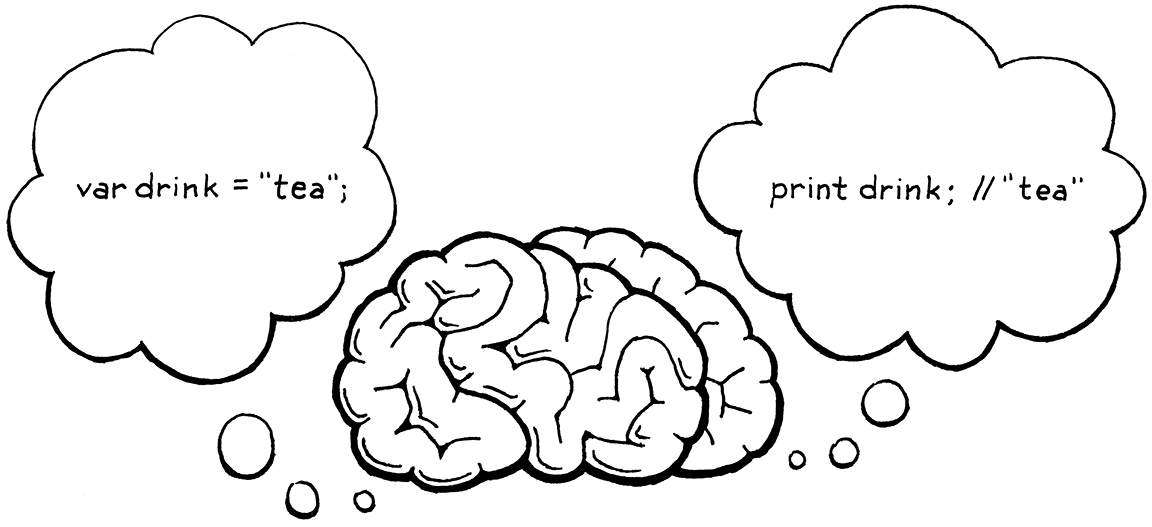
\includegraphics[width=\textwidth]{image/statements-and-state/brain.png}
\end{figure}

状态和语句是相辅相成的。因为根据定义,语句不会计算出一个具体值,而是需要做一些事情来发挥作用。这些事情被称为\textbf{副作用(side effect)}。它可能意味着产生用户可见的输出,或者修改解释器中的一些状态,而这些状态后续可以被检测到。第二个特性使得语句非常适合于定义变量或其他命名实体。

在这一章中,我们会实现所有这些。我们会定义可以产生输出和创建状态的语句,然后会添加表达式来访问和赋值给这些变量,最后,我们会引入代码块和局部作用域。这一章要讲的内容太多了,但是我们会一点一点地把它们嚼碎。

\section{语句}

我们首先扩展Lox的语法以支持语句。 语句与表达式并没有很大的不同,我们从两种最简单的类型开始:

\begin{enumerate}
  \item \textbf{表达式语句}可以让您将表达式放在需要语句的位置。它们的存在是为了计算有副作用的表达式。您可能没有注意到它们,但其实你在C、Java和其他语言中一直在使用表达式语句。如果你看到一个函数或方法调用后面跟着一个;,您看到的其实就是一个表达式语句。
  \item \textbf{print语句}会计算一个表达式,并将结果展示给用户。我承认把print直接放进语言中,而不是把它变成一个库函数,这很奇怪。这样做是基于本书的编排策略的让步,即我们会以章节为单位逐步构建这个解释器,并希望能够在完成解释器的所有功能之前能够使用它。如果让print成为一个标准库函数,我们必须等到拥有了定义和调用函数的所有机制之后,才能看到它发挥作用。
\end{enumerate}

新的词法意味着新的语法规则。在本章中,我们终于获得了解析整个Lox脚本的能力。由于Lox是一种命令式的、动态类型的语言,所以脚本的“顶层”也只是一组语句。新的规则如下:

\begin{ebnf}
program        & \rightarrow\quad statement* \quad EOF \quad ; \\
\\
statement      & \rightarrow\quad \quad exprStmt \\
               & \;\;\vert\quad printStmt \quad ; \\
\\
exprStmt       & \rightarrow\quad expression \mathtt{"};\mathtt{"} \quad ; \\
printStmt      & \rightarrow\quad \mathtt{"}print\mathtt{"} expression \mathtt{"};\mathtt{"} \quad ;
\end{ebnf}

现在第一条规则是program,这也是语法的起点,代表一个完整的Lox脚本或REPL输入项。程序是一个语句列表,后面跟着特殊的“文件结束”(EOF)标记。强制性的结束标记可以确保解析器能够消费所有输入内容,而不会默默地忽略脚本结尾处错误的、未消耗的标记。

目前,statement只有两种情况,分别对应于我们描述的两类语句。我们将在本章后面和接下来的章节中补充更多内容。接下来就是将这个语法转化为我们可以存储在内存中的东西——语法树。。

\subsection{Statement语法树}

语法中没有地方既允许使用表达式,也允许使用语句。操作符(如+)的操作数总是表达式,而不是语句。while循环的主体总是一个语句。

因为这两种语法是不相干的,所以我们不需要提供一个它们都继承的基类。将表达式和语句拆分为单独的类结构,可使Java编译器帮助我们发现一些愚蠢的错误,例如将语句传递给需要表达式的Java方法。

这意味着要为语句创建一个新的基类。正如我们的前辈那样,我们将使用“Stmt”这个隐秘的名字。我很有远见,在设计我们的AST元编程脚本时就已经预见到了这一点。这就是为什么我们把“Expr”作为参数传给了defineAst()。现在我们添加另一个方法调用来定义Stmt和它的子类。

\begin{code}{java}{}{tool/GenerateAst.java,在main()方法中新增:}
      "Unary    : Token operator, Expr right"
    ));
    
    defineAst(outputDir, "Stmt", Arrays.asList(
      "Expression : Expr expression",
      "Print      : Expr expression"
    ));
  }
\end{code}

新节点对应的生成代码可以参考附录: 附录2:Expression statement,Print statement。

运行AST生成器脚本,查看生成的Stmt.java文件,其中包含表达式和print语句所需的语法树类。不要忘记将该文件添加到IDE项目或makefile或其他文件中。

\subsection{解析语句}

解析器的parse()方法会解析并返回一个表达式,这是一个临时方案,是为了让上一章的代码能启动并运行起来。现在,我们的语法已经有了正确的起始规则,即program,我们可以正式编写parse()方法了。

\begin{code}{java}{}{lox/Parser.java,parse()方法,替换7行:}
  List<Stmt> parse() {
    List<Stmt> statements = new ArrayList<>();
    while (!isAtEnd()) {
      statements.add(statement());
    }

    return statements; 
  }
\end{code}

该方法会尽可能多地解析一系列语句,直到命中输入内容的结尾为止。这是一种非常直接的将program规则转换为递归下降风格的方式。由于我们现在使用ArrayList,所以我们还必须向Java的冗长之神做一个小小的祈祷。

\begin{code}{java}{2}{lox/Parser.java,新增代码:}
package com.craftinginterpreters.lox;
import java.util.ArrayList;
import java.util.List;
\end{code}

一个程序就是一系列的语句,而我们可以通过下面的方法解析每一条语句:

\begin{code}{java}{}{lox/Parser.java,在expression()方法后添加}
  private Stmt statement() {
    if (match(PRINT)) return printStatement();

    return expressionStatement();
  }
\end{code}

这是一个简单的框架,但是稍后我们将会填充更多的语句类型。我们通过查看当前标记来确定匹配哪条语句规则。print标记意味着它显然是一个print语句。

如果下一个标记看起来不像任何已知类型的语句,我们就认为它一定是一个表达式语句。这是解析语句时典型的最终失败分支,因为我们很难通过第一个标记主动识别出一个表达式。

每种语句类型都有自己的方法。首先是print:

\begin{code}{java}{}{lox/Parser.java,在statement()方法后添加}
  private Stmt printStatement() {
    Expr value = expression();
    consume(SEMICOLON, "Expect ';' after value.");
    return new Stmt.Print(value);
  }
\end{code}

因为我们已经匹配并消费了print标记本身,所以这里不需要重复消费。我们先解析随后的表达式,消费表示语句终止的分号,并生成语法树。

如果我们没有匹配到print语句,那一定是一条下面的语句:

\begin{code}{java}{}{lox/Parser.java,在printStatement()方法后添加}
  private Stmt expressionStatement() {
    Expr expr = expression();
    consume(SEMICOLON, "Expect ';' after expression.");
    return new Stmt.Expression(expr);
  }
\end{code}

与前面的方法类似,我们解析一个后面带分号的表达式。我们将Expr封装在一个正确类型的Stmt中,并返回它。

\subsection{执行语句}

我们在前面几章一步一步地慢慢完成了解释器的前端工作。我们的解析器现在可以产生语句语法树,所以下一步,也是最后一步,就是对其进行解释。和表达式一样,我们使用的是Visitor模式,但是我们需要实现一个新的访问者接口Stmt.Visitor,因为语句有自己的基类。

我们将其添加到Interpreter实现的接口列表中。

\begin{code}{java}{1-2}{lox/Interpreter.java,替换1行:}
class Interpreter implements Expr.Visitor<Object>,
                             Stmt.Visitor<Void> {
  void interpret(Expr expression) { 
\end{code}

与表达式不同,语句不会产生值,因此visit方法的返回类型是Void,而不是Object。我们有两种语句类型,每种类型都需要一个visit方法。最简单的是表达式语句:

\begin{code}{java}{}{lox/Interpreter.java,在evaluate()方法后添加}
  @Override
  public Void visitExpressionStmt(Stmt.Expression stmt) {
    evaluate(stmt.expression);
    return null;
  }
\end{code}

我们使用现有的evaluate()方法计算内部表达式,并丢弃其结果值。然后我们返回null,因为Java要求为特殊的大写Void返回类型返回该值。很奇怪,但你能有什么办法呢?

print语句的visit方法没有太大的不同。

\begin{code}{java}{}{lox/Interpreter.java,在visitExpressionStmt()方法后添加}
  @Override
  public Void visitPrintStmt(Stmt.Print stmt) {
    Object value = evaluate(stmt.expression);
    System.out.println(stringify(value));
    return null;
  }
\end{code}

在丢弃表达式的值之前,我们使用上一章引入的stringify()方法将其转换为字符串,然后将其输出到stdout。

我们的解释器现在可以处理语句了,但是我们还需要做一些工作将语句输入到解释器中。首先,修改Interpreter类中原有的interpret() 方法,让其能够接受一组语句——即一段程序。

\begin{code}{java}{}{lox/Interpreter.java,修改interpret()方法,替换8行:}
  void interpret(List<Stmt> statements) {
    try {
      for (Stmt statement : statements) {
        execute(statement);
      }
    } catch (RuntimeError error) {
      Lox.runtimeError(error);
    }
  }
\end{code}

这段代码替换了原先处理单个表达式的旧代码。新代码依赖于下面的小辅助方法。

\begin{code}{java}{}{lox/Interpreter.java,在evaluate()方法后添加}
  private void execute(Stmt stmt) {
    stmt.accept(this);
  }
\end{code}

这类似于处理表达式的evaluate()方法,这是这里处理语句。因为我们要使用列表,所以我们需要在Java中引入一下。

\begin{code}{java}{2}{lox/Interpreter.java}
package com.craftinginterpreters.lox;
import java.util.List;
class Interpreter implements Expr.Visitor<Object>,
\end{code}

Lox主类中仍然是只解析单个表达式并将其传给解释器。我们将其修正如下:

\begin{code}{java}{2}{lox/Lox.java,在run()方法中替换1行:}
    Parser parser = new Parser(tokens);
    List<Stmt> statements = parser.parse();
    // Stop if there was a syntax error.
\end{code}

然后将对解释器的调用替换如下:

\begin{code}{java}{2}{lox/Lox.java,在run()方法中替换1行:}
    if (hadError) return;
    interpreter.interpret(statements);
  }
\end{code}

基本就是对新语法进行遍历。好的,启动解释器并测试一下。现在有必要在文本文件中草拟一个小的Lox程序来作为脚本运行。 就像是:

\begin{code}{js}{}{}
print "one";
print true;
print 2 + 1;
\end{code}

它看起来就像一个真实的程序! 请注意,REPL现在也要求你输入完整的语句,而不是简单的表达式。所以不要忘记后面的分号。

\section{全局变量}

现在我们已经有了语句,可以开始出了状态了。在深入探讨语法作用域的复杂性之前,我们先从最简单的变量(全局变量)开始。我们需要两个新的结构。

\begin{enumerate}
  \item \textbf{变量声明}语句用于创建一个新变量。
   
   \begin{code}{js}{}{}
   var beverage = "espresso";
   \end{code}
   
   该语句将创建一个新的绑定,将一个名称(这里是beverage)和一个值(这里是字符串"espresso")关联起来。
   
  \item 一旦声明完成,\textbf{变量表达式}就可以访问该绑定。当标识符“beverage”被用作一个表达式时,程序会查找与该名称绑定的值并返回。
   
   \begin{code}{js}{}{}
   print beverage; // "espresso".
   \end{code}
\end{enumerate}

稍后,我们会添加赋值和块作用域,但是这些已经足够继续后面的学习了。

\subsection{变量语法}

与前面一样,我们将从语法开始,从前到后依次完成实现。变量声明是一种语句,但它们不同于其他语句,我们把statement语法一分为二来处理该情况。这是因为语法要限制某个位置上哪些类型的语句是被允许的。

控制流语句中的子句——比如,if或while语句体中的then和else分支——都是一个语句。但是这个语句不应该是一个声明名称的语句。下面的代码是OK的:

\begin{code}{java}{}{}
if (monday) print "Ugh, already?";
\end{code}

但是下面的代码不行:

\begin{code}{java}{}{}
if (monday) var beverage = "espresso";
\end{code}

我们也\textit{可以}允许后者,但是会令人困惑。beverage变量的作用域是什么?if语句结束之后它是否还继续存在?如果存在的话,在其它条件下它的值是什么?这个变量是否在其它情形下也一直存在?

这样的代码有点奇怪,所以C、Java及类似语言中都不允许这种写法。语句就好像有两个“优先级”。有些允许语句的地方——比如在代码块内或程序顶层——可以允许任何类型的语句,包括变量声明。而其他地方只允许那些不声明名称的、优先级更高的语句。

为了适应这种区别,我们为声明名称的语句类型添加了另一条规则:

\begin{ebnf}
program        \rightarrow\quad declaration* EOF ; \\
\\
declaration    \rightarrow\quad varDecl \\
               \;\;\vert \quad statement \quad ; \\
\\
statement      \rightarrow\quad exprStmt \\
               \;\;\vert \quad printStmt ;
\end{ebnf}

声明语句属于新的declaration规则。目前,这里只有变量,但是后面还会包含函数和类。任何允许声明的地方都允许一个非声明式的语句,所以declaration规则会下降到statement。显然,你可以在脚本的顶层声明一些内容,所以program规则需要路由到新规则。

声明一个变量的规则如下:

\begin{ebnf}
varDecl \rightarrow \quad \mathtt{"}var\mathtt{"} \quad IDENTIFIER \quad ( \quad \mathtt{"}=\mathtt{"} \quad expression \quad )? \quad \mathtt{"};\mathtt{"} \quad ;
\end{ebnf}

像大多数语句一样,它以一个前置关键字开头,这里是var。然后是一个标识符标记,作为声明变量的名称,后面是一个可选的初始化式表达式。最后,以一个分号作为结尾。

为了访问变量,我们还需要定义一个新类型的基本表达式:

\begin{ebnf}
primary &\rightarrow\quad \mathtt{"}true\mathtt{"} \quad\vert\quad \mathtt{"}false\mathtt{"} \quad\vert\quad \mathtt{"}nil\mathtt{"} \\
&\;\;\vert\quad NUMBER \quad\vert\quad STRING \\
&\;\;\vert\quad \mathtt{"}(\mathtt{"} expression \mathtt{"})\mathtt{"} \\
&\;\;\vert\quad IDENTIFIER \quad ;
\end{ebnf}

IDENTIFIER子语句会匹配单个标识符标记,该标记会被理解为正在访问的变量的名称。

这些新的语法规则需要其相应的语法树。在AST生成器中,我们为变量声明添加一个新的语句树。

\begin{code}{java}{3}{tool/GenerateAst.java,在main()方法中添加1行,前1行需要加,:}
      "Expression : Expr expression",
      "Print      : Expr expression",
      "Var        : Token name, Expr initializer"
    ));
\end{code}

这里存储了名称标记,以便我们知道该语句声明了什么,此外还有初始化表达式(如果没有,字段就是null)。

然后我们添加一个表达式节点用于访问变量。

\begin{code}{js}{3}{tool/GenerateAst.java,在main()方法中添加1行,前1行需要加“,”}
      "Literal  : Object value",
      "Unary    : Token operator, Expr right",
      "Variable : Token name"
    ));
\end{code}

这只是对变量名称标记的简单包装,就是这样。像往常一样,别忘了运行AST生成器脚本,这样你就能得到更新的“Expr.java”和“Stmt.java”文件。

\subsection{解析变量}

在解析变量语句之前,我们需要修改一些代码,为语法中的新规则declaration腾出一些空间。现在,程序的最顶层是声明语句的列表,所以解析器方法的入口需要更改:

\begin{code}{java}{4}{lox/Parser.java,在parse()方法中替换1行:}
    List<Stmt> parse() {
    List<Stmt> statements = new ArrayList<>();
    while (!isAtEnd()) {  
      statements.add(declaration());
    }

    return statements; 
  }
\end{code}

这里会调用下面的新方法:

\begin{code}{java}{}{lox/Parser.java,在expression()方法后添加}
  private Stmt declaration() {
    try {
      if (match(VAR)) return varDeclaration();

      return statement();
    } catch (ParseError error) {
      synchronize();
      return null;
    }
  }
\end{code}

你还记得前面的章节中,我们建立了一个进行错误恢复的框架吗?现在我们终于可以用起来了。

当我们解析块或脚本中的一系列语句时,declaration()方法会被重复调用。因此当解析器进入恐慌模式时,它就是进行同步的正确位置。该方法的整个主体都封装在一个try块中,以捕获解析器开始错误恢复时抛出的异常。这样可以让解析器跳转到解析下一个语句或声明的开头。

真正的解析工作发生在try块中。首先,它通过查找前面的var关键字判断是否是变量声明语句。如果不是的话,就会进入已有的statement()方法中,解析print和语句表达式。

还记得statement()会在没有其它语句匹配时会尝试解析一个表达式语句吗?而expression()如果无法在当前语法标记处解析表达式,则会抛出一个语法错误?这一系列调用链可以保证在解析无效的声明或语句时会报告错误。

当解析器匹配到一个var标记时,它会跳转到:

\begin{code}{java}{}{lox/Parser.java,在printStatement()方法后添加}
  private Stmt varDeclaration() {
    Token name = consume(IDENTIFIER, "Expect variable name.");

    Expr initializer = null;
    if (match(EQUAL)) {
      initializer = expression();
    }

    consume(SEMICOLON, "Expect ';' after variable declaration.");
    return new Stmt.Var(name, initializer);
  }
\end{code}

与之前一样,递归下降代码会遵循语法规则。解析器已经匹配了var标记,所以接下来要消费一个标识符标记作为变量的名称。

然后,如果找到=标记,解析器就知道后面有一个初始化表达式,并对其进行解析。否则,它会将初始器保持为null。最后,会消费语句末尾所需的分号。然后将所有这些都封装到一个Stmt.Var语法树节点中。

解析变量表达式甚至更简单。在primary()中,我们需要查找一个标识符标记。

\begin{code}{java}{3-5}{lox/Parser.java,在primary()方法中添加}
      return new Expr.Literal(previous().literal);
    }
    if (match(IDENTIFIER)) {
      return new Expr.Variable(previous());
    }
    if (match(LEFT_PAREN)) {
\end{code}

这为我们提供了声明和使用变量的可用前端,剩下的就是将其接入解释器中。在此之前,我们需要讨论变量在内存中的位置。

\section{环境}

变量与值之间的绑定关系需要保存在某个地方。自从Lisp发明圆括号以来,这种数据结构就被称为\textbf{环境}。

\begin{figure}[htbp]
  \centering
  
\includegraphics[width=\textwidth]{image/statements-and-state/environment.png}
\end{figure}

你可以把它想象成一个映射,其中键是变量名称,值就是变量的值。实际上,这也就是我们在Java中采用的实现方式。我们可以直接在解释器中加入该映射及其管理代码,但是因为它形成了一个很好的概念,我们可以将其提取到单独的类中。

\begin{code}{java}{}{打开新文件,添加以下代码:}
package com.craftinginterpreters.lox;

import java.util.HashMap;
import java.util.Map;

class Environment {
  private final Map<String, Object> values = new HashMap<>();
}
\end{code}

其中使用一个Java Map来保存绑定关系。这里使用原生字符串作为键,而不是使用标记。一个标记表示源文本中特定位置的一个代码单元,但是在查找变量时,具有相同名称的标识符标记都应该指向相同的变量(暂时忽略作用域)。使用原生字符串可以保证所有这些标记都会指向相同的映射键。

我们需要支持两个操作。首先,是变量定义操作,可以将一个新的名称与一个值进行绑定。

\begin{code}{java}{}{lox/Environment.java,在Environment类中添加}
  void define(String name, Object value) {
    values.put(name, value);
  }
\end{code}

不算困难,但是我们这里也做出了一个有趣的语义抉择。当我们向映射中添加键时,没有检查该键是否已存在。这意味着下面的代码是有效的:

\begin{code}{js}{}{}
var a = "before";
print a; // "before".
var a = "after";
print a; // "after".
\end{code}

变量语句不仅可以定义一个新变量,也可以用于重新定义一个已有的变量。我们可以选择将其作为一个错误来处理。用户可能不打算重新定义已有的变量(如果他们想这样做,可能会使用赋值,而不是var),将重定义作为错误可以帮助用户发现这个问题。

然而,这样做与REPL的交互很差。在与REPL的交互中,最好是让用户不必在脑子记录已经定义了哪些变量。我们可以在REPL中允许重定义,在脚本中不允许。但是这样一来,用户就不得不学习两套规则,而且一种形式的代码复制粘贴到另一种形式后可能无法运行。

所以,为了保证两种模式的统一,我们选择允许重定义——至少对于全局变量如此。一旦一个变量存在,我们就需要可以查找该变量的方法。

\begin{code}{java}{3-10}{lox/Environment.java,在Environment类中添加}
class Environment {
  private final Map<String, Object> values = new HashMap<>();
  Object get(Token name) {
    if (values.containsKey(name.lexeme)) {
      return values.get(name.lexeme);
    }

    throw new RuntimeError(name,
        "Undefined variable '" + name.lexeme + "'.");
  }
  void define(String name, Object value) {
\end{code}

这在语义上更有趣一些。如果找到了这个变量,只需要返回与之绑定的值。但如果没有找到呢?我们又需要做一个选择:

\begin{itemize}
  \item 抛出语法错误
  \item 抛出运行时错误
  \item 允许该操作并返回默认值(如nil)
\end{itemize}

Lox是很宽松的,但最后一个选项对我来说有点过于宽松了。把它作为语法错误(一个编译时的错误)似乎是一个明智的选择。使用未定义的变量确实是一个错误,用户越早发现这个错误就越好。

问题在于,\textit{使用}一个变量并不等同于\textit{引用}它。如果代码块封装在函数中,则可以在代码块中引用变量,而不必立即对其求值。如果我们把引用未声明的变量当作一个静态错误,那么定义递归函数就变得更加困难了。

通过在检查函数体之前先声明函数名称,我们可以支持单一递归——调用自身的函数。但是,这无法处理互相调用的递归程序。考虑以下代码:

\begin{code}{js}{}{}
fun isOdd(n) {
  if (n == 0) return false;
  return isEven(n - 1);
}

fun isEven(n) {
  if (n == 0) return true;
  return isOdd(n - 1);
}
\end{code}

当我们查看isOdd()方法时,isEven()方法被调用的时候还没有被声明。如果我们交换着两个函数的顺序,那么在查看isEven()方法体时会发现isOdd()方法未被定义。

因为将其当作\textit{静态}错误会使递归声明过于困难,因此我们把这个错误推迟到运行时。在一个变量被定义之前引用它是可以的,只要你不对引用进行\textit{求值}。这样可以让前面的奇偶数代码正常工作。但是执行以下代码时,你会得到一个运行时错误:

\begin{code}{js}{}{}
print a;
var a = "too late!";
\end{code}

与表达式计算代码中的类型错误一样,我们通过抛出一个异常来报告运行时错误。异常中包含变量的标记,以便我们告诉用户代码的什么位置出现了错误。

\subsection{解释全局变量}

Interpreter类会获取Environment类的一个实例。

\begin{code}{java}{3}{lox/Interpreter.java,在Interpreter类中添加}
class Interpreter implements Expr.Visitor<Object>,
                             Stmt.Visitor<Void> {  
  private Environment environment = new Environment();
  void interpret(List<Stmt> statements) {
\end{code}

我们直接将它作为一个字段存储在解释器中,这样,只要解释器仍在运行,变量就会留在内存中。

我们有两个新的语法树,所以这就是两个新的访问方法。第一个是关于声明语句的。

\begin{code}{java}{}{lox/Interpreter.java,在visitPrintStmt()方法后添加}
  @Override
  public Void visitVarStmt(Stmt.Var stmt) {
    Object value = null;
    if (stmt.initializer != null) {
      value = evaluate(stmt.initializer);
    }

    environment.define(stmt.name.lexeme, value);
    return null;
  }
\end{code}

如果该变量有初始化式,我们就对其求值。如果没有,我们就需要做一个选择。我们可以通过在解析器中\textit{要求}初始化式令其成为一个语法错误。但是,大多数语言都不会这么做,所以在Lox中这样做感觉有点苛刻。

我们可以使其成为运行时错误。我们允许您定义一个未初始化的变量,但如果您在对其赋值之前访问它,就会发生运行时错误。这不是一个坏主意,但是大多数动态类型的语言都不会这样做。相反,我们使用最简单的方式。或者说,如果变量没有被显式初始化,Lox会将变量设置为nil。

\begin{code}{js}{}{}
var a;
print a; // "nil".
\end{code}

因此,如果没有初始化式,我们将值设为null,这也是Lox中的nil值的Java表示形式。然后,我们告诉环境上下文将变量与该值进行绑定。

接下来,我们要对变量表达式求值。

\begin{code}{java}{}{lox/Interpreter.java,在visitUnaryExpr()方法后添加}
  @Override
  public Object visitVariableExpr(Expr.Variable expr) {
    return environment.get(expr.name);
  }
\end{code}

这里只是简单地将操作转发到环境上下文中,环境做了一些繁重的工作保证变量已被定义。这样,我们就可以支持基本的变量操作了。尝试以下代码:

\begin{code}{js}{}{}
var a = 1;
var b = 2;
print a + b;
\end{code}

我们还不能复用代码,但是我们可以构建能够复用数据的程序。

\section{赋值}

你可以创建一种语言,其中有变量,但是不支持对该变量重新赋值(或更改)。Haskell就是一个例子。SML只支持可变引用和数组——变量不能被重新赋值。Rust则通过要求mut标识符开启赋值,从而引导用户远离可更改变量。

更改变量是一种副作用,顾名思义,一些语言专家认为副作用是肮脏或不优雅的。代码应该是纯粹的数学,它会产生值——纯净的、不变的值——就像上帝造物一样。而不是一些肮脏的自动机器,将数据块转换成各种形式,一次执行一条命令。

Lox没有这么严苛。Lox是一个命令式语言,可变性是与生俱来的,添加对赋值操作的支持并不需要太多工作。全局变量已经支持了重定义,所以该机制的大部分功能已经存在。主要的是,我们缺少显式的赋值符号。

\subsection{赋值语法}

这个小小的=语法比看起来要更复杂。像大多数C派生语言一样,赋值是一个表达式,而不是一个语句。和C语言中一样,它是优先级最低的表达式形式。这意味着该规则在语法中处于 expression 和equality(下一个优先级的表达式)之间。

\begin{ebnf}
expression & \rightarrow\quad assignment \quad ; \\
assignment & \rightarrow\quad IDENTIFIER \quad \mathtt{"}=\mathtt{"} \quad assignment \\
& \;\;\vert\quad equality \quad ;
\end{ebnf}

这就是说,一个assignment(赋值式)要么是一个标识符,后跟一个=和一个对应值的表达式;要么是一个等式(也就是任何其它)表达式。稍后,当我们在对象中添加属性设置式时,赋值将会变得更加复杂,比如:

\begin{code}{java}{}{}
instance.field = "value";
\end{code}

最简单的部分就是添加新的语法树节点。

\begin{code}{java}{2}{tool/GenerateAst.java,在main()方法中添加}
    defineAst(outputDir, "Expr", Arrays.asList(
      "Assign   : Token name, Expr value",
      "Binary   : Expr left, Token operator, Expr right",
\end{code}

其中包含被赋值变量的标记,一个计算新值的表达式。运行AstGenerator得到新的Expr.Assign类之后,替换掉解析器中现有的expression()方法的方法体,以匹配最新的规则。

\begin{code}{java}{2}{lox/Parser.java,在expression()方法中替换1行:}
  private Expr expression() {
    return assignment();
  }
\end{code}

这里开始变得棘手。单个标记前瞻递归下降解析器直到解析完左侧标记并且遇到=标记\textit{之后},才能判断出来正在解析的是赋值语句。你可能会想,为什么需要这样做?毕竟,我们也是完成左操作数的解析之后才知道正在解析的是+表达式。

区别在于,赋值表达式的左侧不是可以求值的表达式,而是一种伪表达式,计算出的是一个你可以赋值的“东西”。考虑以下代码:

\begin{code}{js}{}{}
var a = "before";
a = "value";
\end{code}

在第二行中,我们不会对a进行求值(如果求值会返回“before”)。我们要弄清楚a指向的是什么变量,这样我们就知道该在哪里保存右侧表达式的值。这两个概念的经典术语是\textbf{左值}和\textbf{右值}。到目前为止,我们看到的所有产生值的表达式都是右值。左值“计算”会得到一个存储位置,你可以向其赋值。

我们希望语法树能够反映出左值不会像常规表达式那样计算。这也是为什么Expr.Assign节点的左侧是一个Token,而不是Expr。问题在于,解析器直到遇到等号“=”才知道正在解析一个左值。在一个复杂的左值中,可能在出现很多标记之后才能识别到。

\begin{code}{java}{}{}
makeList().head.next = node;
\end{code}

我们只会前瞻一个标记,那我们该怎么办呢?我们使用一个小技巧,看起来像下面这样:

\begin{code}{java}{}{lox/Parser.java,在expressionStatement()方法后添加}
  private Expr assignment() {
    Expr expr = equality();

    if (match(EQUAL)) {
      Token equals = previous();
      Expr value = assignment();

      if (expr instanceof Expr.Variable) {
        Token name = ((Expr.Variable)expr).name;
        return new Expr.Assign(name, value);
      }

      error(equals, "Invalid assignment target."); 
    }

    return expr;
  }
\end{code}

解析赋值表达式的大部分代码看起来与解析其它二元运算符(如+)的代码类似。我们解析左边的内容,它可以是任何优先级更高的表达式。如果我们发现一个=,就解析右侧内容,并把它们封装到一个复杂表达式树节点中。

与二元运算符的一个细微差别在于,我们不会循环构建相同操作符的序列。因为赋值操作是右关联的,所以我们递归调用assignment()来解析右侧的值。

诀窍在于,在创建赋值表达式节点之前,我们先查看左边的表达式,弄清楚它是什么类型的赋值目标。然后我们将右值表达式节点转换为左值的表示形式。

这种转换是有效的,因为事实证明,每个有效的赋值目标正好也是符合普通表达式的有效语法。考虑一个复杂的属性赋值操作,如下:

\begin{code}{java}{}{}
newPoint(x + 2, 0).y = 3;
\end{code}

该赋值表达式的左侧也是一个有效的表达式。

\begin{code}{java}{}{}
newPoint(x + 2, 0).y;
\end{code}

第一个例子设置该字段,第二个例子获取该字段。

这意味着,我们可以像解析表达式一样解析左侧内容,然后生成一个语法树,将其转换为赋值目标。如果左边的表达式不是一个有效的赋值目标,就会出现一个语法错误。这样可以确保在遇到类似下面的代码时会报告错误:

\begin{code}{java}{}{}
a + b = c;
\end{code}

现在,唯一有效的赋值目标就是一个简单的变量表达式,但是我们后面会添加属性字段。这个技巧的最终结果是一个赋值表达式树节点,该节点知道要向什么赋值,并且有一个表达式子树用于计算要使用的值。所有这些都只用了一个前瞻标记,并且没有回溯。

\subsection{赋值的语义}

我们有了一个新的语法树节点,所以我们的解释器也需要一个新的访问方法。

\begin{code}{java}{}{lox/Interpreter.java,在visitVarStmt()方法后添加}
  @Override
  public Object visitAssignExpr(Expr.Assign expr) {
    Object value = evaluate(expr.value);
    environment.assign(expr.name, value);
    return value;
  }
\end{code}

很明显,这与变量声明很类似。首先,对右侧表达式运算以获取值,然后将其保存到命名变量中。这里不使用Environment中的define(),而是调用下面的新方法:

\begin{code}{java}{}{lox/Environment.java,在get()方法后添加}
  void assign(Token name, Object value) {
    if (values.containsKey(name.lexeme)) {
      values.put(name.lexeme, value);
      return;
    }

    throw new RuntimeError(name,
        "Undefined variable '" + name.lexeme + "'.");
  }
\end{code}

赋值与定义的主要区别在于,赋值操作不允许创建新变量。就我们的实现而言,这意味着如果环境的变量映射中不存在变量的键,那就是一个运行时错误。

visit()方法做的最后一件事就是返回要赋给变量的值。这是因为赋值是一个表达式,可以嵌套在其他表达式里面,就像这样:

\begin{code}{js}{}{}
var a = 1;
print a = 2; // "2".
\end{code}

我们的解释器现在可以创建、读取和修改变量。这和早期的BASIC一样复杂。全局变量很简单,但是在编写一个大型程序时,任何两块代码都可能不小心修改对方的状态,这就不好玩了。我们需要\textit{局部}变量,这意味着是时候讨论\textit{作用域}了。

\section{作用域}

\textbf{作用域}定义了名称映射到特定实体的一个区域。多个作用域允许同一个名称在不同的上下文中指向不同的内容。在我家,“Bob”通常指的是我自己,但是在你的身边,你可能人数另外一个Bob。相同的名字,基于你的所知所见指向了不同的人。

\textbf{词法作用域}(或者比较少见的\textbf{静态作用域})是一种特殊的作用域定义方式,程序本身的文本显示了作用域的开始和结束位置。Lox,和大多数现代语言一样,变量在词法作用域内有效。当你看到使用了某些变量的表达式时,你通过静态地阅读代码就可以确定其指向的变量声明。

举例来说:

\begin{code}{js}{}{}
{
  var a = "first";
  print a; // "first".
}

{
  var a = "second";
  print a; // "second".
}
\end{code}

这里,我们在两个块中都定义了一个变量a。我们可以从代码中看出,在第一个print语句中使用的a指的是第一个a,第二个语句指向的是第二个变量。

\begin{figure}[htbp]
  \centering
  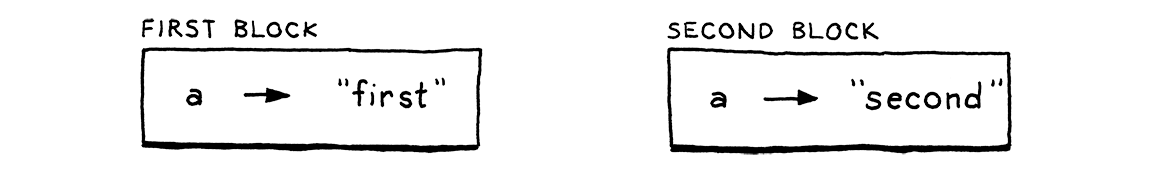
\includegraphics[width=\textwidth]{image/statements-and-state/blocks.png}
\end{figure}

这与\textbf{动态作用域}形成了对比,在动态作用域中,直到执行代码时才知道名称指向的是什么。Lox没有动态作用域\textit{变量},但是对象上的方法和字段是动态作用域的。

\begin{code}{java}{}{}
class Saxophone {
  play() {
    print "Careless Whisper";
  }
}

class GolfClub {
  play() {
    print "Fore!";
  }
}

fun playIt(thing) {
  thing.play();
}
\end{code}

当playIt()调用thing.play()时,我们不知道我们将要听到的是“Careless Whisper”还是“Fore!”。这取决于你向函数传递的是Saxophone还是GolfClub,而我们在运行时才知道这一点。

作用域和环境是近亲,前者是理论概念,而后者是实现它的机制。当我们的解释器处理代码时,影响作用域的语法树节点会改变环境上下文。在像Lox这样的类C语言语法中,作用域是由花括号的块控制的。(这就是为什么我们称它为\textbf{块范围})。

\begin{code}{js}{}{}
{
  var a = "in block";
}
print a; // Error! No more "a".
\end{code}

块的开始引入了一个新的局部作用域,当执行通过结束的\}时,这个作用域就结束了。块内声明的任何变量都会消失。

\subsection{嵌套和遮蔽}

实现块作用域的第一步可能是这样的:

\begin{enumerate}
  \item 当访问块内的每个语句时,跟踪所有声明的变量。
  \item 执行完最后一条语句后,告诉环境将这些变量全部删除。
\end{enumerate}

这对前面的例子是可行的。但是请记住,局部作用域的一个目的是封装——程序中一个块内的代码,不应该干扰其他代码块。看看下面的例子:

\begin{code}{js}{}{}
// How loud?
var volume = 11;

// Silence.
volume = 0;

// Calculate size of 3x4x5 cuboid.
{
  var volume = 3 * 4 * 5;
  print volume;
}
\end{code}

请看这个代码块,在这里我们声明了一个局部变量volume来计算长方体的体积。该代码块退出后,解释器将删除\textit{全局}volume变量。这是不对的。当我们退出代码块时,我们应该删除在块内声明的所有变量,但是如果在代码块外声明了相同名称的变量,那就是一个不同的变量。它不应该被删除。

当局部变量与外围作用域中的变量具有相同的名称时,内部变量会遮蔽外部变量。代码块内部不能再看到外部变量——它被遮蔽在内部变量的阴影中——但它仍然是存在的。

当进入一个新的块作用域时,我们需要保留在外部作用域中定义的变量,这样当我们退出内部代码块时这些外部变量仍然存在。为此,我们为每个代码块定义一个新的环境,该环境只包含该作用域中定义的变量。当我们退出代码块时,我们将丢弃其环境并恢复前一个环境。

我们还需要处理没有被遮蔽的外围变量。

\begin{code}{js}{}{}
var global = "outside";
{
  var local = "inside";
  print global + local;
}
\end{code}

这段代码中,global在外部全局环境中,local则在块环境中定义。在执行print语句时,这两个变量都在作用域内。为了找到它们,解释器不仅要搜索当前最内层的环境,还必须搜索所以外围的环境。

我们通过将环境链接在一起来实现这一点。每个环境都有一个对直接外围作用域的环境的引用。当我们查找一个变量时,我们从最内层开始遍历环境链直到找到该变量。从内部作用域开始,就是我们使局部变量遮蔽外部变量的方式。

\begin{figure}[htbp]
  \centering
  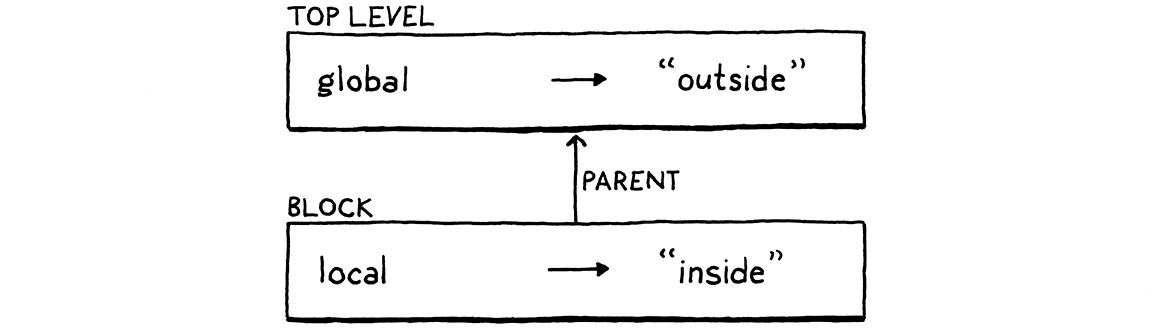
\includegraphics[width=\textwidth]{image/statements-and-state/chaining.png}
\end{figure}

在我们添加块语法之前,我们要强化Environment类对这种嵌套的支持。首先,我们在每个环境中添加一个对其外围环境的引用。

\begin{code}{java}{2}{lox/Environment.java,在Environment类中添加}
class Environment {
  final Environment enclosing;
  private final Map<String, Object> values = new HashMap<>();
\end{code}

这个字段需要初始化,所以我们添加两个构造函数。

\begin{code}{java}{}{lox/Environment.java,在Environment类中添加}
  Environment() {
    enclosing = null;
  }

  Environment(Environment enclosing) {
    this.enclosing = enclosing;
  }
\end{code}

无参构造函数用于全局作用域环境,它是环境链的结束点。另一个构造函数用来创建一个嵌套在给定外部作用域内的新的局部作用域。

我们不必修改define()方法——因为新变量总是在当前最内层的作用域中声明。但是变量的查找和赋值是结合已有的变量一起处理的,需要遍历环境链以找到它们。首先是查找操作:

\begin{code}{java}{3}{lox/Environment.java,在get()方法中添加}
      return values.get(name.lexeme);
    }
    if (enclosing != null) return enclosing.get(name);
    throw new RuntimeError(name,
        "Undefined variable '" + name.lexeme + "'.");
\end{code}

如果当前环境中没有找到变量,就在外围环境中尝试。然后递归地重复该操作,最终会遍历完整个链路。如果我们到达了一个没有外围环境的环境,并且仍然没有找到这个变量,那我们就放弃,并且像之前一样报告一个错误。

赋值也是如此。

\begin{code}{java}{4-7}{lox/Environment.java,在assign()方法中添加}
      values.put(name.lexeme, value);
      return;
    }
    if (enclosing != null) {
      enclosing.assign(name, value);
      return;
    }
    throw new RuntimeError(name,
\end{code}

同样,如果变量不在此环境中,它会递归地检查外围环境。

\subsection{块语法和语义}

现在环境已经嵌套了,我们就准备向语言中添加块了。请看以下语法:

\begin{ebnf}
statement &\rightarrow\quad exprStmt \\
& \;\;\vert\quad printStmt \\
& \;\;\vert\quad block \quad ; \\
\\
block &\rightarrow\quad \mathtt{"}{\mathtt{"} \quad declaration* \quad \mathtt{"}}\mathtt{"} \quad ;
\end{ebnf}

块是由花括号包围的一系列语句或声明(可能是空的)。块本身就是一条语句,可以出现在任何允许语句的地方。语法树节点如下所示。

\begin{code}{java}{2}{tool/GenerateAst.java,在main()方法中添加}
    defineAst(outputDir, "Stmt", Arrays.asList(
      "Block      : List<Stmt> statements",
      "Expression : Expr expression",
\end{code}

它包含块中语句的列表。解析很简单。与其他语句一样,我们通过块的前缀标记(在本例中是{)来检测块的开始。在statement()方法中,我们添加代码:

\begin{code}{java}{2}{lox/Parser.java,在statement()方法中添加}
    if (match(PRINT)) return printStatement();
    if (match(LEFT_BRACE)) return new Stmt.Block(block());
    return expressionStatement();
\end{code}

真正的工作都在这里进行:

\begin{code}{java}{}{lox/Parser.java,在expressionStatement()方法后添加}
  private List<Stmt> block() {
    List<Stmt> statements = new ArrayList<>();

    while (!check(RIGHT_BRACE) && !isAtEnd()) {
      statements.add(declaration());
    }

    consume(RIGHT_BRACE, "Expect '}' after block.");
    return statements;
  }
\end{code}

我们先创建一个空列表,然后解析语句并将其放入列表中,直至遇到块的结尾(由\}符号标识)。注意,该循环还有一个明确的isAtEnd()检查。我们必须小心避免无限循环,即使在解析无效代码时也是如此。如果用户忘记了结尾的\},解析器需要保证不能被阻塞。

语法到此为止。对于语义,我们要在Interpreter中添加另一个访问方法。

\begin{code}{java}{}{lox/Interpreter.java,在execute()方法后添加}
  @Override
  public Void visitBlockStmt(Stmt.Block stmt) {
    executeBlock(stmt.statements, new Environment(environment));
    return null;
  }
\end{code}

要执行一个块,我们先为该块作用域创建一个新的环境,然后将其传入下面这个方法:

\begin{code}{java}{}{lox/Interpreter.java,在execute()方法后添加}
  void executeBlock(List<Stmt> statements,
                    Environment environment) {
    Environment previous = this.environment;
    try {
      this.environment = environment;

      for (Stmt statement : statements) {
        execute(statement);
      }
    } finally {
      this.environment = previous;
    }
  }
\end{code}

这个新方法会在给定的环境上下文中执行一系列语句。在此之前,解释器中的environment字段总是指向相同的环境——全局环境。现在,这个字段会指向\textit{当前}环境,也就是与要执行的代码的最内层作用域相对应的环境。

为了在给定作用域内执行代码,该方法会先更新解释器的environment字段,执行所有的语句,然后恢复之前的环境。基于Java中一贯的优良传统,它使用finally子句来恢复先前的环境。这样一来,即使抛出了异常,环境也会被恢复。

出乎意料的是,这就是我们为了完全支持局部变量、嵌套和遮蔽所需要做的全部事情。试运行下面的代码:

\begin{code}{js}{}{}
var a = "global a";
var b = "global b";
var c = "global c";
{
  var a = "outer a";
  var b = "outer b";
  {
    var a = "inner a";
    print a;
    print b;
    print c;
  }
  print a;
  print b;
  print c;
}
print a;
print b;
print c;
\end{code}

我们的小解释器现在可以记住东西了,我们举例全功能编程语言又近了一步。

\section{挑战}

\begin{enumerate}
  \item REPL不再支持输入一个表达式并自动打印其结果值。这是个累赘。在REPL中增加支持,让用户既可以输入语句又可以输入表达式。如果他们输入一个语句,就执行它。如果他们输入一个表达式,则对表达式求值并显示结果值。
  \item 也许你希望Lox对变量的初始化更明确一些。与其隐式地将变量初始化为nil,不如将访问一个未被初始化或赋值的变量作为一个运行时错误,如:

\begin{code}{js}{}{}
// No initializers.
var a;
var b;

a = "assigned";
print a; // OK, was assigned first.

print b; // Error!
\end{code}

  \item 下面的代码会怎么执行?

\begin{code}{js}{}{}
var a = 1;
{
  var a = a + 2;
  print a;
}
\end{code}

你期望它怎么执行?它是按照你的想法执行的吗?你所熟悉的其他语言中的类似代码怎么执行?你认为用户会期望它怎么执行?
\end{enumerate}

\section{设计笔记:隐式变量声明}

Lox使用不同的语法来声明新变量和为已有变量赋值。有些语言将其简化为只有赋值语法。对一个不存在的变量进行赋值时会自动生成该变量。这被称为\textbf{隐式变量声明},存在于Python、Ruby和CoffeeScript以及其他语言中。JavaScript有一个显式的语法来声明变量,但是也可以在赋值时创建新变量。Visual Basic有一个选项可以启用或禁用隐式变量。

当同样的语法既可以对变量赋值,也可以创建变量时,语言实现就必须决定在不清楚用户的预期行为时该怎么办。特别是,每种语言必须选择隐式变量声明与变量遮蔽的交互方式,以及隐式变量应该属于哪个作用域。

\begin{itemize}
  \item 在Python中,赋值总是会在当前函数的作用域内创建一个变量,即使在函数外部声明了同名变量。
  \item Ruby通过对局部变量和全局变量使用不同的命名规则,避免了一些歧义。但是,Ruby中的块(更像闭包,而不是C中的“块”)具有自己的作用域,因此仍然存在问题。在Ruby中,如果已经存在一个同名的变量,则赋值会赋给当前块之外的现有变量。否则,就会在当前块的作用域中创建一个新变量。
  \item CoffeeScript在许多方面都效仿Ruby,这一点也类似。它明确禁止变量遮蔽,要求赋值时总是优先赋给外部作用域中现有的变量(一直到最外层的全局作用域)。如果变量不存在的话,它会在当前函数作用域中创建新变量。
  \item 在JavaScript中,赋值会修改任意外部作用域中的一个现有变量(如果能找到该变量的话)。如果变量不存在,它就隐式地在全局作用域内创建一个新的变量。
\end{itemize}

隐式声明的主要优点是简单。语法较少,无需学习“声明”概念。用户可以直接开始赋值,然后语言就能解决其它问题。

像C这样较早的静态类型语言受益于显式声明,是因为它们给用户提供了一个地方,让他们告诉编译器每个变量的类型以及为它分配多少存储空间。在动态类型、垃圾收集的语言中,这其实是没有必要的,所以你可以通过隐式声明来实现。这感觉更“脚本化”,更像是“你懂我的意思吧”。

但这是就个好主意吗?隐式声明还存在一些问题。

\begin{itemize}
  \item 用户可能打算为现有变量赋值,但是出现拼写错误。解释器不知道这一点,所以它悄悄地创建了一些新变量,而用户想要赋值的变量仍然是原来的值。这在JavaScript中尤其令人讨厌,因为一个拼写错误会创建一个全局变量,这反过来又可能会干扰其它代码。
  \item JS、Ruby和CoffeeScript通过判断是否存在同名变量——包括外部作用域——来确定赋值是创建新变量还是赋值给现有变量。这意味着在外围作用域中添加一个新变量可能会改变现有代码的含义,原先的局部变量可能会默默地变成对新的外部变量的赋值。
  \item 在Python中,你可能想要赋值给当前函数之外的某个变量,而不是在当前函数中创建一个新变量,但是你做不到。
\end{itemize}

随着时间的推移,我所知道的具有隐式变量声明的语言最后都增加了更多的功能和复杂性来处理这些问题。

\begin{itemize}
  \item 现在,普遍认为JavaScript中全局变量的隐式声明是一个错误。“strict mode”禁用了它,并将其成为一个编译错误。
  \item Python添加了一个global语句,让用户可以在函数内部显式地赋值给一个全局变量。后来,随着函数式编程和嵌套函数越来越流行,他们添加了一个类似的nonlocal语句来赋值给外围函数中的变量。
  \item Ruby扩展了它的块语法,允许在块中显式地声明某些变量,即使外部作用域中存在同名的变量。
\end{itemize}

考虑到这些,我认为简单性的论点已经失去了意义。有一种观点认为隐式声明是正确的默认选项,但我个人认为这种说法不太有说服力。

我的观点是,隐式声明在过去的几年里是有意义的,当时大多数脚本语言都是非常命令式的,代码是相当简单直观的。随着程序员对深度嵌套、函数式编程和闭包越来越熟悉,访问外部作用域中的变量变得越来越普遍。这使得用户更有可能遇到棘手的情况,即不清楚他们的赋值是要创建一个新变量还是重用外围的已有变量。

所以我更喜欢显式声明变量,这就是为什么Lox要这样做的原因。

\chapter{控制流}

\epigraph{逻辑和威士忌一样,如果摄入太多,就是失去其有益的效果。}{爱德华}

与上一章艰苦的马拉松相比,这一章就是在雏菊草地上的轻松嬉戏。虽然工作很简单,但回报却惊人的大。

现在,我们的解释器只不过是一个计算器而已。一个Lox程序在结束之前只能做固定的工作量。要想让它的运行时间延长一倍,你就必须让源代码的长度增加一倍。我们即将解决这个问题。在本章中,我们的解释器向编程语言大联盟迈出了一大步:图灵完备性。

\section{图灵机(简介)}

在上世纪初,数学家们陷入了一系列令人困惑的悖论之中,导致他们对自己工作所依赖的基础的稳定性产生怀疑。为了解决这一危机,他们又回到了原点。他们希望从少量的公理、逻辑和集合理论开始,在一个不透水的地基上重建数学。

他们想要严格地回答这样的问题:“所有真实的陈述都可以被证明吗?”,“我们可以计算我们能定义的所有函数吗?”,甚至是更一般性的问题,“当我们声称一个函数是'可计算的'时,代表什么意思?”

他们认为前两个问题的答案应该是“是”,剩下的就是去证明它。但事实证明这两个问题的答案都是“否”。而且令人惊讶的是,这两个问题是深深地交织在一起的。这是数学的一个迷人的角落,它触及了关于大脑能够做什么和宇宙如何运作的基本问题。我在这里说不清楚。

我想指出的是,在证明前两个问题的答案是“否”的过程中,艾伦·图灵和阿隆佐·邱奇为最后一个问题设计了一个精确的答案,即定义了什么样的函数是可计算的。他们各自设计了一个具有最小机械集的微型系统,该系统仍然强大到足以计算一个超大类函数中的任何一个。

这些现在被认为是“可计算函数”。图灵的系统被称为\textbf{图灵机},邱奇的系统是\textbf{lambda演算}。这两种方法仍然被广泛用作计算模型的基础,事实上,许多现代函数式编程语言的核心都是lambda演算。

\begin{figure}[htbp]
  \centering
  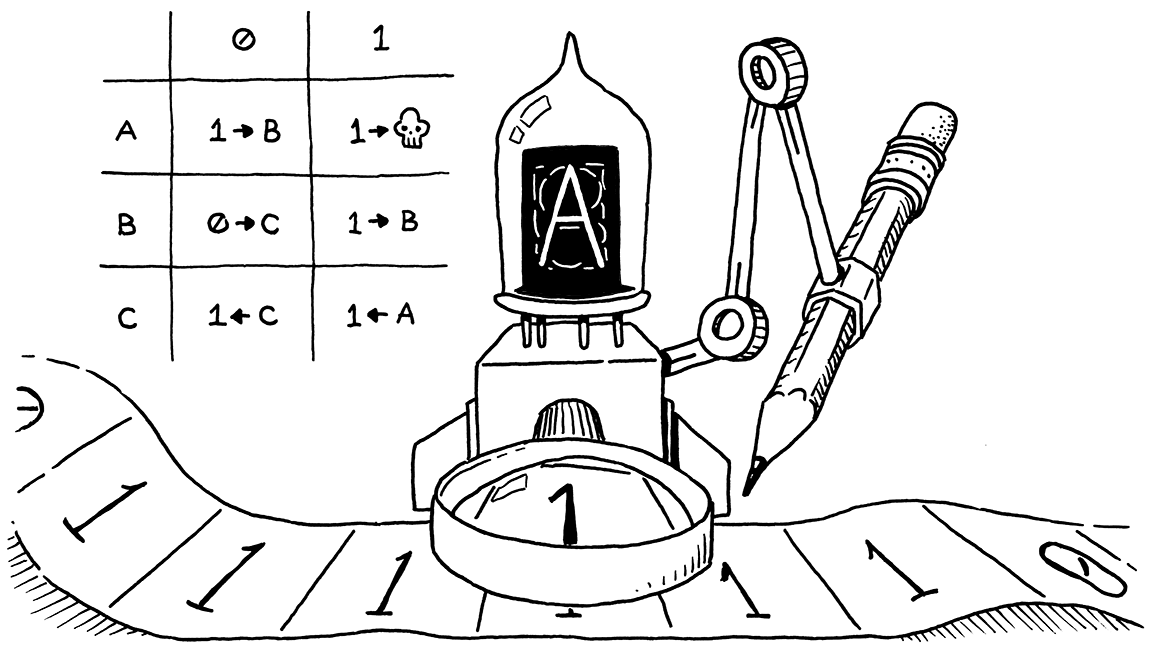
\includegraphics[width=\textwidth]{image/control-flow/turing-machine.png}
\end{figure}

图灵机的知名度更高——目前还没有关于阿隆佐·邱奇的好莱坞电影,但这两种形式在能力上是等价的。事实上,任何具有最低表达能力的编程语言都足以计算任何可计算函数。

你可以用自己的语言为图灵机编写一个模拟器来证明这一点。由于图灵证明了他的机器可以计算任何可计算函数,推而广之,这意味着你的语言也可以。你所需要做的就是把函数翻译成图灵机,然后在你的模拟器上运行它。

如果你的语言有足够的表达能力来做到这一点,它就被认为是\textbf{图灵完备}的。图灵机非常简单,所以它不需要太多的能力。您基本上只需要算术、一点控制流以及分配和使用(理论上)任意数量内存的能力。我们已经具备了第一个条件。在本章结束时,我们将具备第二个条件。

\section{条件执行}

说完了历史,现在让我们把语言优化一下。我们大致可以把控制流分为两类:

\begin{itemize}
  \item \textbf{条件}或\textbf{分支控制流}是用来不执行某些代码的。意思是,你可以把它看作是跳过了代码的一个区域。
  \item \textbf{循环控制流}是用于多次执行一块代码的。它会\textit{向回}跳转,从而能再次执行某些代码。用户通常不需要无限循环,所以一般也会有一些条件逻辑用于判断何时停止循环。
\end{itemize}

分支更简单一些,所以我们先从分支开始实现。C衍生语言中包含两个主要的条件执行功能,即if语句和“条件”运算符(?:)。if语句使你可以按条件执行语句,而条件运算符使你可以按条件执行表达式。

为了简单起见,Lox没有条件运算符,所以让我们直接开始if语句吧。我们的语句语法需要一个新的生成式。

\begin{ebnf}
statement &\rightarrow\quad exprStmt \\
&\;\;\vert\quad ifStmt \\
&\;\;\vert\quad printStmt \\
&\;\;\vert\quad block ; \\
\\
ifStmt &\rightarrow\quad \mathtt{"}if\mathtt{"} \quad \mathtt{"}(\mathtt{"} \quad expression \quad \mathtt{"})\mathtt{"} \quad statement \\
& \quad\quad ( \quad \mathtt{"}else\mathtt{"} \quad statement \quad )? \quad ;
\end{ebnf}

if语句有一个表达式作为条件,然后是一个在条件为真时要执行的语句。另外,它还可以有一个else关键字和条件为假时要执行的语句。语法树节点中对语法的这三部分都有对应的字段。

\begin{code}{java}{2-3}{tool/GenerateAst.java,在main()方法中添加}
      "Expression : Expr expression",
      "If         : Expr condition, Stmt thenBranch," +
                  " Stmt elseBranch",
      "Print      : Expr expression",
\end{code}

与其它语句类似,解析器通过开头的if关键字来识别if语句。

\begin{code}{java}{2}{lox/Parser.java,在statement()方法中添加}
  private Stmt statement() {
    if (match(IF)) return ifStatement();
    if (match(PRINT)) return printStatement();
\end{code}

如果发现了if关键字,就调用下面的新方法解析其余部分:

\begin{code}{java}{}{lox/Parser.java,在statement()方法后添加}
  private Stmt ifStatement() {
    consume(LEFT_PAREN, "Expect '(' after 'if'.");
    Expr condition = expression();
    consume(RIGHT_PAREN, "Expect ')' after if condition."); 

    Stmt thenBranch = statement();
    Stmt elseBranch = null;
    if (match(ELSE)) {
      elseBranch = statement();
    }

    return new Stmt.If(condition, thenBranch, elseBranch);
  }
\end{code}

跟之前一样,解析代码严格遵循语法。它通过查找前面的else关键字来检测else子句。如果没有,语法树中的elseBranch字段为null。

实际上,这个看似无伤大雅的可选项在我们的语法中造成了歧义。考虑以下代码:

\begin{code}{js}{}{}
if (first) if (second) whenTrue(); else whenFalse();
\end{code}

谜题是这样的:这里的else子句属于哪个if语句?这不仅仅是一个关于如何标注语法的理论问题。它实际上会影响代码的执行方式:

\begin{itemize}
  \item 如果我们将else语句关联到第一个if语句,那么当first为假时,无论second的值是多少,都将调用whenFalse()。
  \item 如果我们将else语句关联到第二个if语句,那么只有当first为假并且second也为假时,才会调用whenFalse()。
\end{itemize}

由于else子句是可选的,而且没有明确的分隔符来标记if语句的结尾,所以当你以这种方式嵌套if时,语法是不明确的。这种典型的语法陷阱被称为悬空的else问题。

\begin{figure}[htbp]
  \centering
  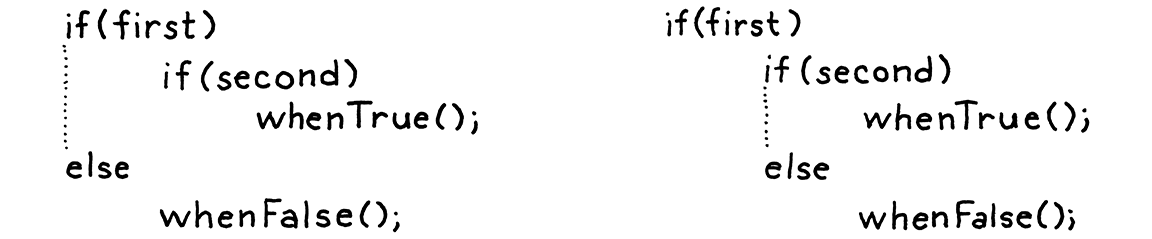
\includegraphics[width=\textwidth]{image/control-flow/dangling-else.png}
\end{figure}

也可以定义一个上下文无关的语法来直接避免歧义,但是需要将大部分语句规则拆分成对,一个是允许带有else的if语句,另一个不允许。这很烦人。

相反,大多数语言和解析器都以一种特殊的方式避免了这个问题。不管他们用什么方法来解决这个问题,他们总是选择同样的解释——else与前面最近的if绑定在一起。

我们的解析器已经很方便地做到了这一点。因为ifStatement()在返回之前会继续寻找一个else子句,连续嵌套的最内层调用在返回外部的if语句之前,会先为自己声明else语句。

语法就绪了,我们可以开始解释了。

\begin{code}{java}{}{lox/Interpreter.java,在visitExpressionStmt()后添加}
  @Override
  public Void visitIfStmt(Stmt.If stmt) {
    if (isTruthy(evaluate(stmt.condition))) {
      execute(stmt.thenBranch);
    } else if (stmt.elseBranch != null) {
      execute(stmt.elseBranch);
    }
    return null;
  }
\end{code}

解释器实现就是对相同的Java代码的简单包装。它首先对条件表达式进行求值。如果为真,则执行then分支。否则,如果有存在else分支,就执行该分支。

如果你把这段代码与解释器中我们已实现的处理其它语法的代码进行比较,会发现控制流中特殊的地方就在于Java的if语句。其它大多数语法树总是会对子树求值,但是这里,我们可能会不执行then语句或else语句。如果其中任何一个语句有副作用,那么选择不执行某条语句就是用户可见的。

\section{逻辑操作符}

由于我们没有条件运算符,你可能认为我们已经完成分支开发了,但其实还没有。虽然没有三元运算符,但是还有两个其它操作符在技术上是控制流结构——逻辑运算符and和or。

它们与其它二进制运算符不同,是因为它们会短路。如果在计算左操作数之后,我们已经确切知道逻辑表达式的结果,那么就不再计算右操作数。例如:

\begin{code}{js}{}{}
false and sideEffect();
\end{code}

对于一个and表达式来说,两个操作数都必须是真,才能得到结果为真。我们只要看到左侧的false操作数,就知道结果不会是真,也就不需要对sideEffect()求值,会直接跳过它。

这就是为什么我们没有在实现其它二元运算符的时候一起实现逻辑运算符。现在我们已经准备好了。这两个新的运算符在优先级表中的位置很低,类似于C语言中的||和\&\&,它们都有各自的优先级,or低于and。我们把这两个运算符插入assignment 和 equality之间。

\begin{ebnf}
expression &\rightarrow\quad assignment \quad ; \\
assignment &\rightarrow\quad IDENTIFIER \quad \mathtt{"}=\mathtt{"} \quad assignment \\
          &\;\;\vert\quad logic\_or \quad ; \\
logic\_or  &\rightarrow\quad logic\_and \quad ( \quad \mathtt{"}or\mathtt{"} \quad logic\_and \quad )* \quad ; \\
logic\_and &\rightarrow\quad equality \quad ( \quad \mathtt{"}and\mathtt{"} \quad equality \quad )* \quad ;
\end{ebnf}

assignment现在不是落到equality,而是继续进入logic\_or。两个新规则,logic\_or 和logic\_and,与其它二元运算符类似。然后logic\_and会调用equality计算其操作数,然后我们就链入了表达式规则的其它部分。

对于这两个新表达式,我们可以重用Expr.Binary类,因为他们具有相同的字段。但是这样的话,visitBinaryExpr()方法中必须检查运算符是否是逻辑运算符,并且要使用不同的代码处理短路逻辑。我认为更整洁的方法是为这些运算符定义一个新类,这样它们就有了自己的visit方法。

\begin{code}{java}{2}{tool/GenerateAst.java,在main()方法中添加}
      "Literal  : Object value",
      "Logical  : Expr left, Token operator, Expr right",
      "Unary    : Token operator, Expr right",
\end{code}

为了将新的表达式加入到解析器中,我们首先将赋值操作的解析代码改为调用or()方法。

\begin{code}{java}{2}{lox/Parser.java,在assignment()方法中替换1行:}
  private Expr assignment() {
    Expr expr = or();
    if (match(EQUAL)) {
\end{code}

解析一系列or语句的代码与其它二元运算符相似。

\begin{code}{java}{}{lox/Parser.java,在assignment()方法后添加}
  private Expr or() {
    Expr expr = and();

    while (match(OR)) {
      Token operator = previous();
      Expr right = and();
      expr = new Expr.Logical(expr, operator, right);
    }

    return expr;
  }
\end{code}

它的操作数是位于下一优先级的新的and表达式。

\begin{code}{java}{}{lox/Parser.java,在or()方法后添加}
  private Expr and() {
    Expr expr = equality();

    while (match(AND)) {
      Token operator = previous();
      Expr right = equality();
      expr = new Expr.Logical(expr, operator, right);
    }

    return expr;
  }
\end{code}

这里会调用equality()计算操作数,这样一来,表达式解析器又重新绑定到了一起。我们已经准备好进行解释了。

\begin{code}{java}{}{lox/Interpreter.java,在visitLiteralExpr()方法后添加}
  @Override
  public Object visitLogicalExpr(Expr.Logical expr) {
    Object left = evaluate(expr.left);

    if (expr.operator.type == TokenType.OR) {
      if (isTruthy(left)) return left;
    } else {
      if (!isTruthy(left)) return left;
    }

    return evaluate(expr.right);
  }
\end{code}

如果你把这个方法与前面章节的visitBinaryExpr()方法相比较,就可以看出其中的区别。这里,我们先计算左操作数。然后我们查看结果值,判断是否可以短路。当且仅当不能短路时,我们才计算右侧的操作数。

另一个有趣的部分是决定返回什么实际值。由于Lox是动态类型的,我们允许任何类型的操作数,并使用真实性来确定每个操作数代表什么。我们对结果采用类似的推理。逻辑运算符并不承诺会真正返回true或false,而只是保证它将返回一个具有适当真实性的值。

幸运的是,我们手边就有具有适当真实性的值——即操作数本身的结果,所以我们可以直接使用它们。如:

\begin{code}{js}{}{}
print "hi" or 2; // "hi".
print nil or "yes"; // "yes".
\end{code}

在第一行,“hi”是真的,所以or短路并返回它。在第二行,nil是假的,因此它计算并返回第二个操作数“yes”。

这样就完成了Lox中的所有分支原语,我们准备实现循环吧。

\section{While循环}

Lox有两种类型的循环控制流语句,分别是while和for。while循环更简单一点,我们先从它开始.

\begin{ebnf}
statement &\rightarrow\quad exprStmt \\
&\;\;\vert\quad ifStmt \\
&\;\;\vert\quad printStmt \\
&\;\;\vert\quad whileStmt \\
&\;\;\vert\quad block \quad ; \\
\\
whileStmt &\rightarrow\quad \mathtt{"}while\mathtt{"} \quad \mathtt{"}(\mathtt{"} \quad expression \quad \mathtt{"})\mathtt{"} \quad statement \quad ;
\end{ebnf}

我们在statement规则中添加一个子句,指向while对应的新规则whileStmt。该规则接收一个while关键字,后跟一个带括号的条件表达式,然后是循环体对应的语句。新语法规则需要定义新的语法树节点。

\begin{code}{java}{3}{tool/GenerateAst.java,在main()方法中新增,前1行后添加“,”}
      "Print      : Expr expression",
      "Var        : Token name, Expr initializer",
      "While      : Expr condition, Stmt body"
    ));
\end{code}

该节点中保存了条件式和循环体。这里就可以看出来为什么表达式和语句最好要有单独的基类。字段声明清楚地表明了,条件是一个表达式,循环主体是一个语句。

在解析器中,我们遵循与if语句相同的处理步骤。首先,在statement()添加一个case分支检查并匹配开头的关键字。

\begin{code}{java}{2}{lox/Parser.java,在statement()方法中添加}
    if (match(PRINT)) return printStatement();
    if (match(WHILE)) return whileStatement();
    if (match(LEFT_BRACE)) return new Stmt.Block(block());
\end{code}

实际的工作委托给下面的方法:

\begin{code}{java}{}{lox/Parser.java,在varDeclaration()方法后添加}
  private Stmt whileStatement() {
    consume(LEFT_PAREN, "Expect '(' after 'while'.");
    Expr condition = expression();
    consume(RIGHT_PAREN, "Expect ')' after condition.");
    Stmt body = statement();

    return new Stmt.While(condition, body);
  }
\end{code}

语法非常简单,这里将其直接翻译为Java。说到直接翻译成Java,下面是我们执行新语法的方式:

\begin{code}{java}{}{lox/Interpreter.java,在visitVarStmt()方法后添加}
  @Override
  public Void visitWhileStmt(Stmt.While stmt) {
    while (isTruthy(evaluate(stmt.condition))) {
      execute(stmt.body);
    }
    return null;
  }
\end{code}

和if的访问方法一样,这里的访问方法使用了相应的Java特性。这个方法并不复杂,但它使Lox变得更加强大。我们终于可以编写一个运行时间不受源代码长度严格限制的程序了。

\section{For循环}

我们已经到了最后一个控制流结构,即老式的C语言风格for循环。我可能不需要提醒你,但还是要说它看起来是这样的: 

\begin{code}{js}{}{}
for (var i = 0; i < 10; i = i + 1) print i;
\end{code}

在语法中,是这样的:

\begin{ebnf}
statement &\rightarrow\quad exprStmt \\
&\;\;\vert\quad forStmt \\
&\;\;\vert\quad ifStmt \\
&\;\;\vert\quad printStmt \\
&\;\;\vert\quad whileStmt \\
&\;\;\vert\quad block \quad ; \\
\\
forStmt &\rightarrow\quad \mathtt{"}for\mathtt{"} \quad \mathtt{"}(\mathtt{"} \quad ( \quad varDecl \quad\vert\quad exprStmt \quad\vert\quad \mathtt{"};\mathtt{"} \quad ) \\
& \quad\quad expression? \quad \mathtt{"};\mathtt{"} \\
& \quad\quad expression? \mathtt{"})\mathtt{"} \quad statement \quad ;
\end{ebnf}

在括号内,有三个由分号分隔的子语句:

\begin{enumerate}
  \item 第一个子句是\textit{初始化式}。它只会在任何其它操作之前执行一次。它通常是一个表达式,但是为了便利,我们也允许一个变量声明。在这种情况下,变量的作用域就是for循环的其它部分——其余两个子式和循环体。
  \item 接下来是\textit{条件表达式}。与while循环一样,这个表达式控制了何时退出循环。它会在每次循环开始之前执行一次(包括第一次)。如果结果是真,就执行循环体;否则,就结束循环。
  \item 最后一个子句是\textit{增量式}。它是一个任意的表达式,会在每次循环结束的时候做一些工作。因为表达式的结果会被丢弃,所以它必须有副作用才能有用。在实践中,它通常会对变量进行递增。
\end{enumerate}

这些子语句都可以忽略。在右括号之后是一个语句作为循环体,通常是一个代码块。

\subsection{语法脱糖}

这里包含了很多配件,但是请注意,它所做的任何事情中,没有一件是无法用已有的语句实现的。如果for循环不支持初始化子句,你可以在for语句之前加一条初始化表达式。如果没有增量子语句,你可以直接把增量表达式放在循环体的最后。

换句话说,Lox不\textit{需要}for循环,它们只是让一些常见的代码模式更容易编写。这类功能被称为\textbf{语法糖}。例如,前面的for循环可以改写成这样:

\begin{code}{js}{}{}
{
  var i = 0;
  while (i < 10) {
    print i;
    i = i + 1;
  }
}
\end{code}

虽然这个脚本不太容易看懂,但这个脚本与之前那个语义完全相同。像Lox中的for循环这样的语法糖特性可以使语言编写起来更加愉快和高效。但是,特别是在复杂的语言实现中,每一个需要后端支持和优化的语言特性都是代价昂贵的。

我们可以通过\textbf{脱糖}来吃这个蛋糕。这个有趣的词描述了这样一个过程:前端接收使用了语法糖的代码,并将其转换成后端知道如何执行的更原始的形式。

我们将把for循环脱糖为while循环和其它解释器可处理的其它语句。在我们的简单解释器中,脱糖真的不能为我们节省很多工作,但它确实给了我一个契机来向你介绍这一技术。因此,与之前的语句不同,我们不会为for循环添加一个新的语法树节点。相反,我们会直接进行解析。首先,先引入一个我们要用到的依赖:

\begin{code}{java}{2}{lox/Parser.java,添加代码:}
import java.util.ArrayList;
import java.util.Arrays;
import java.util.List;
\end{code}

像每个语句一样,我们通过匹配for关键字来解析循环。

\begin{code}{java}{2}{lox/Parser.java,在statement()方法中新增:}
  private Stmt statement() {
    if (match(FOR)) return forStatement();
    if (match(IF)) return ifStatement();
\end{code}

接下来是有趣的部分,脱糖也是在这里发生的,所以我们会一点点构建这个方法,首先从子句之前的左括号开始。

\begin{code}{java}{}{lox/Parser.java,在statement()方法后添加}
  private Stmt forStatement() {
    consume(LEFT_PAREN, "Expect '(' after 'for'.");

    // More here...
  }
\end{code}

接下来的第一个子句是初始化式。

\begin{code}{java}{2-9}{lox/Parser.java,在forStatement()方法中替换1行:}
    consume(LEFT_PAREN, "Expect '(' after 'for'.");
    Stmt initializer;
    if (match(SEMICOLON)) {
      initializer = null;
    } else if (match(VAR)) {
      initializer = varDeclaration();
    } else {
      initializer = expressionStatement();
    }
  }
\end{code}

如果(后面的标记是分号,name初始化式就被省略了。否则,我们就检查var关键字,看它是否是一个变量声明。如果这两者都不符合,那么它一定是一个表达式。我们对其进行解析,并将其封装在一个表达式语句中,这样初始化器就必定属于Stmt类型。

接下来是条件表达式。

\begin{code}{java}{3-7}{lox/Parser.java,在forStatement()方法中添加代码:}
      initializer = expressionStatement();
    }
    Expr condition = null;
    if (!check(SEMICOLON)) {
      condition = expression();
    }
    consume(SEMICOLON, "Expect ';' after loop condition.");
  }
\end{code}

同样,我们查找分号检查子句是否被忽略。最后一个子句是增量语句。

\begin{code}{java}{2-6}{lox/Parser.java,在forStatement()方法中添加}
    consume(SEMICOLON, "Expect ';' after loop condition.");
    Expr increment = null;
    if (!check(RIGHT_PAREN)) {
      increment = expression();
    }
    consume(RIGHT_PAREN, "Expect ')' after for clauses.");
  }
\end{code}

它类似于条件式子句,只是这个子句是由右括号终止的。剩下的就是循环主体了。

\begin{code}{java}{2-4}{lox/Parser.java,在forStatement()方法中添加代码:}
    consume(RIGHT_PAREN, "Expect ')' after for clauses.");
    Stmt body = statement();

    return body;
  }
\end{code}

我们已经解析了for循环的所有部分,得到的AST节点也存储在一些Java本地变量中。这里也是脱糖开始的地方。我们利用这些变量来合成表示for循环语义的语法树节点,就像前面展示的手工脱糖的例子一样。

如果我们向后向前处理,代码会更简单一些,所以我们从增量子句开始。

\begin{code}{java}{2-7}{lox/Parser.java,在forStatement()方法中新增:}
    Stmt body = statement();
    if (increment != null) {
      body = new Stmt.Block(
          Arrays.asList(
              body,
              new Stmt.Expression(increment)));
    }
    return body;
\end{code}

如果存在增量子句的话,会在循环的每个迭代中在循环体结束之后执行。我们用一个代码块来代替循环体,这个代码块中包含原始的循环体,后面跟一个执行增量子语句的表达式语句。

\begin{code}{java}{2-3}{lox/Parser.java,在forStatement()方法中新增代码:}
    }
    if (condition == null) condition = new Expr.Literal(true);
    body = new Stmt.While(condition, body);
    return body;
\end{code}

接下来,我们获取条件式和循环体,并通过基本的while语句构建对应的循环。如果条件式被省略了,我们就使用true来创建一个无限循环。

\begin{code}{java}{2-4}{lox/Parser.java,在forStatement()方法中新增:}
    body = new Stmt.While(condition, body);
    if (initializer != null) {
      body = new Stmt.Block(Arrays.asList(initializer, body));
    }
    return body;
\end{code}

最后,如果有初始化式,它会在整个循环之前运行一次。我们的做法是,再次用代码块来替换整个语句,该代码块中首先运行一个初始化式,然后执行循环。

就是这样。我们的解释器现在已经支持了C语言风格的for循环,而且我们根本不需要修改解释器类。因为我们通过脱糖将其转换为了解释器已经知道如何访问的节点,所以无需做其它的工作。

最后,Lox已强大到足以娱乐我们,至少几分钟。下面是一个打印斐波那契数列前21个元素的小程序:

\begin{code}{js}{}{}
var a = 0;
var temp;

for (var b = 1; a < 10000; b = temp + b) {
  print a;
  temp = a;
  a = b;
}
\end{code}

\section{挑战}

\begin{enumerate}
  \item 在接下来的几章中,当Lox支持一级函数和动态调度时,从技术上讲,我们就不需要在语言中内置分支语句。说明如何用这些特性来实现条件执行。说出一种在控制流中使用这种技术的语言。
  \item 同样地,只要我们的解释器支持一个重要的优化,循环也可以用这些工具来实现。它是什么?为什么它是必要的?请说出一种使用这种技术进行迭代的语言。
  \item 与Lox不同,大多数其他C风格语言也支持循环内部的break和continue语句。添加对break语句的支持。
\end{enumerate}

语法是一个break关键字,后面跟一个分号。如果break语句出现在任何封闭的循环之后,那就应该是一个语法错误。在运行时,break语句会跳转到最内层的封闭循环的末尾,并从那里开始继续执行。注意,break语句可以嵌套在其它需要退出的代码块和if语句中。

\section{设计笔记:一些语法糖}

当你设计自己的语言时,你可以选择在语法中注入多少语法糖。你是要做一种不加糖、每个语法操作都对应单一的语法单元的健康食品?还是每一点行为都可以用10种不同方式实现的堕落的甜点?把这两种情况看作是两端的话,成功的语言分布在这个连续体的每个中间点。

极端尖刻的一侧是那些语法极少的语言,如Lisp、Forth和SmallTalk。Lisp的拥趸广泛声称他们的语言 "没有语法",而Smalltalk的人则自豪地表示,你可以把整个语法放在一张索引卡上。这个部落的理念是,语言不需要句法糖。相反,它所提供的最小的语法和语义足够强大,足以让库中的代码像语言本身的一部分一样具有表现力。

接近这些的是像C、Lua和Go这样的语言。他们的目标是简单和清晰,而不是极简主义。有些语言,如Go,故意避开了语法糖和前一类语言的语法扩展性。他们希望语法不受语义的影响,所以他们专注于保持语法和库的简单性。代码应该是明显的,而不是漂亮的。

介于之间的是Java、C\#和Python等语言。最终,你会看到Ruby、C++、Perl和D-语言,它们在语法中塞入了太多的句法规则,以至于键盘上的标点符号都快用完了。

在某种程度上,频谱上的位置与年龄相关。在后续的版本中增加一些语法糖是比较容易的。新的语法很容易让人喜欢,而且与修改语义相比,它更不可能破坏现有的程序。一旦加进去,你就再也不能把它去掉了,所以随着时间的推移,语言会变得越来越甜。从头开始创建一门新语言的主要好处之一是,它给了你一个机会去刮掉那些累积的糖霜并重新开始。

语法糖在PL知识分子中名声不佳。那群人对极简主义有一种真正的迷恋。这是有一定道理的。设计不良的、不必要的语法增加了认知负荷,却没有增加相匹配的表达能力。因为一直会有向语言中添加新特性的压力,所以需要自律并专注于简单,以避免臃肿。一旦你添加了一些语法,你就会被它困住,所以明智的做法是要精简。

同时,大多数成功的语言都有相当复杂的语法,至少在它们被广泛使用的时候是这样。程序员在他们所选择的语言上花费了大量的时间,一些随处可见的细节确实可以提高他们工作时的舒适度和效率。

找到正确的平衡——为你的语言选择适当的甜度——取决于你自己的品味。

\chapter{函数}

\epigraph{这也是人类思维的运作方式——将旧的想法复合成为新结构,成为新的想法,而这些想法本身又可以被用于复合,循环往复,无休无止,越来越远离每一种语言赖以生存的基本的土壤。}{侯世达}

这一章标志着很多艰苦工作的一个高潮。在前面的章节中,各自添加了一些有用的功能,但是每一章也都提供了一个拼图的碎片。我们整理这些碎片——表达式、语句、变量、控制流和词法作用域,再加上其它功能,并把他们组合起来,以支持真正的用户定义函数和函数调用。

\section{函数调用}

你肯定熟悉C语言风格的函数调用语法,但其语法可能比你意识到的更微妙。调用通常是指向命名的函数,例如:

\begin{code}{js}{}{}
average(1, 2);
\end{code}

但是被调用函数的名称实际上并不是调用语法的一部分。被调用者(\textbf{callee})可以是计算结果为一个函数的任何表达式。(好吧,它必须是一个非常高优先级的表达式,但是圆括号可以解决这个问题。)例如:

\begin{code}{js}{}{}
getCallback()();
\end{code}

这里有两个函数调用。第一对括号将getCallback作为其被调用者。但是第二对括号将整个getCallback()表达式作为其被调用者。表达式后面的小括号表示函数调用,你可以把调用看作是一种以(开头的后缀运算符。

这个“运算符”比其它运算符(包括一元运算符)有更高的优先级。所以我们通过让unary规则跳转到新的call规则,将其添加到语法中。

\begin{ebnf}
unary &\rightarrow\quad ( \quad \mathtt{"}!\mathtt{"} \quad\vert\quad \mathtt{"}-\mathtt{"} \quad ) \quad unary \quad\vert\quad call \quad ; \\
call  &\rightarrow\quad primary \quad ( \quad \mathtt{"}(\mathtt{"} \quad arguments? \quad \mathtt{"})\mathtt{"} \quad )* \quad ;
\end{ebnf}

该规则匹配一个基本表达式,后面跟着0个或多个函数调用。如果没有括号,则解析一个简单的基本表达式。否则,每一对圆括号都表示一个函数调用,圆括号内有一个可选的参数列表。参数列表语法是:

\begin{ebnf}
arguments \rightarrow\quad expression \quad ( \quad \mathtt{"},\mathtt{"} \quad expression \quad )* \quad ;
\end{ebnf}

这个规则要求至少有一个参数表达式,后面可以跟0个或多个其它表达式,每两个表达式之间用“,”分隔。为了处理无参调用,call规则本身认为整个arguments生成式是可选的。

我承认,对于极其常见的“零或多个逗号分隔的事物”模式来说,这在语法上似乎比你想象的更难处理。有一些复杂的元语法可以更好地处理这个问题,但在我们的BNF和我见过的许多语言规范中,它就是如此的麻烦。

在我们的语法树生成器中,我们添加一个新节点。

\begin{code}{java}{2}{tool/GenerateAst.java,在main()方法中添加代码:}
      "Binary   : Expr left, Token operator, Expr right",
      "Call     : Expr callee, Token paren, List<Expr> arguments",
      "Grouping : Expr expression",
\end{code}

它存储了被调用者表达式和参数表达式列表,同时也保存了右括号标记。当我们报告由函数调用引起的运行时错误时,会使用该标记的位置。

打开解析器,原来unary()直接跳转到primary()方法,将其修改为调用call()。

\begin{code}{java}{3}{lox/Parser.java,在unary()方法中替换1行:}
      return new Expr.Unary(operator, right);
    }
    return call();
  }
\end{code}

该方法定义为:

\begin{code}{java}{}{lox/Parser.java,在unary()方法后添加}
  private Expr call() {
    Expr expr = primary();

    while (true) { 
      if (match(LEFT_PAREN)) {
        expr = finishCall(expr);
      } else {
        break;
      }
    }

    return expr;
  }
\end{code}

这里的代码与语法规则并非完全一致。为了保持代码简洁,我调整了一些东西——这是我们手写解析器的优点之一。但它与我们解析中缀运算符的方式类似。首先,我们解析一个基本表达式,即调用的左操作数。然后,每次看到(,我们就调用finishCall()解析调用表达式,并使用之前解析出的表达式作为被调用者。返回的表达式成为新的expr,我们循环检查其结果是否被调用。

解析参数列表的代码在下面的工具方法中:

\begin{code}{java}{}{lox/Parser.java,在unary()方法后添加}
  private Expr finishCall(Expr callee) {
    List<Expr> arguments = new ArrayList<>();
    if (!check(RIGHT_PAREN)) {
      do {
        arguments.add(expression());
      } while (match(COMMA));
    }

    Token paren = consume(RIGHT_PAREN,
                          "Expect ')' after arguments.");

    return new Expr.Call(callee, paren, arguments);
  }
\end{code}

这或多或少是arguments语法规则翻译成代码的结果,除了我们这里还处理了无参情况。我们首先判断下一个标记是否)来检查这种情况。如果是,我们就不会尝试解析任何参数。

如果不是,我们就解析一个表达式,然后寻找逗号(表明后面还有一个参数)。只要我们在表达式后面发现逗号,就会继续解析表达式。当我们找不到逗号时,说明参数列表已经结束,我们继续消费预期的右括号。最终,我们将被调用者和这些参数封装成一个函数调用的AST节点。

\subsection{最大参数数量}

现在,我们解析参数的循环是没有边界的。如果你想调用一个函数并向其传递一百万个参数,解析器不会有任何问题。我们要对此进行限制吗?

其它语言采用了不同的策略。C语言标准要求在符合标准的实现中,一个函数至少要支持127个参数,但是没有指定任何上限。Java规范规定一个方法可以接受不超过255个参数。

Lox的Java解释器实际上并不需要限制,但是设置一个最大的参数数量限制可以简化第三部分中的字节码解释器。即使是在这样奇怪的地方里,我们也希望两个解释器能够相互兼容,所以我们为jlox添加同样的限制。

\begin{code}{java}{2-4}{lox/Parser.java,在finishCall()方法中添加}
      do {
        if (arguments.size() >= 255) {
          error(peek(), "Can't have more than 255 arguments.");
        }
        arguments.add(expression());
\end{code}

请注意,如果发现参数过多,这里的代码会\textit{报告}一个错误,但是不会\textit{抛出}该错误。抛出错误是进入恐慌模式的方法,如果解析器处于混乱状态,不知道自己在语法中处于什么位置,那这就是我们想要的。但是在这里,解析器仍然处于完全有效的状态,只是发现了太多的参数。所以它会报告这个错误,并继续执行解析。

\section{解释函数调用}

我们还没有任何可以调用的函数,所以先实现函数调用似乎有点奇怪,但是这个问题我们后面再考虑。首先,我们的解释器需要引入一个新依赖。

\begin{code}{java}{}{lox/Interpreter.java}
import java.util.ArrayList;
import java.util.List;
\end{code}

跟之前一样,解释工作从新的调用表达式节点对应的新的visit方法开始。

\begin{code}{java}{}{lox/Interpreter.java,在visitBinaryExpr()方法后添加}
  @Override
  public Object visitCallExpr(Expr.Call expr) {
    Object callee = evaluate(expr.callee);

    List<Object> arguments = new ArrayList<>();
    for (Expr argument : expr.arguments) { 
      arguments.add(evaluate(argument));
    }

    LoxCallable function = (LoxCallable)callee;
    return function.call(this, arguments);
  }
\end{code}

首先,对被调用者的表达式求值。通常情况下,这个表达式只是一个标识符,可以通过它的名字来查找函数。但它可以是任何东西。然后,我们依次对每个参数表达式求值,并将结果值存储在一个列表中。

一旦我们准备好被调用者和参数,剩下的就是执行函数调用。我们将被调用者转换为LoxCallable,然后对其调用call()方法来实现。任何可以像函数一样被调用的Lox对象的Java表示都要实现这个接口。这自然包括用户定义的函数,但也包括类对象,因为类会被“调用”来创建新的实例。稍后我们还将把它用于另一个目的。

这个新接口中没有太多内容。

\begin{code}{java}{}{lox/LoxCallable.java,创建新文件:}
package com.craftinginterpreters.lox;

import java.util.List;

interface LoxCallable {
  Object call(Interpreter interpreter, List<Object> arguments);
}
\end{code}

我们会传入解释器,以防实现call()方法的类会需要它。我们也会提供已求值的参数值列表。接口实现者的任务就是返回调用表达式产生的值。

\subsection{调用类型错误}

在我们实现LoxCallable之前,我们需要使访问者方法更加健壮一些。现在的访问者方法忽略了很多的错误模式,但我们不能假装没看见。首先,如果被调用的函数根本不是可以调用的呢?如果你像下面这样写代码:

\begin{code}{js}{}{}
"totally not a function"();
\end{code}

在Lox中,字符串是不能被调用的。因为Lox字符串的运行时表示是Java的字符串类型,所以在我们将字符串类型强制转换为LoxCallable接口类型时,JVM将会抛出一个ClassCastException异常。我们不希望解释器输出一些恶心的Java调用栈信息然后死掉。所以,我们首先需要自己来检查一下类型。

\begin{code}{java}{3-6}{lox/Interpreter.java,在visitCallExpr()中添加}
    }

    if (!(callee instanceof LoxCallable)) {
      throw new RuntimeError(expr.paren,
          "Can only call functions and classes.");
    }

    LoxCallable function = (LoxCallable)callee;
\end{code}

\subsection{检查元数}

另一个问题与函数的\textbf{元数}有关。元数是一个花哨的术语,指一个函数或操作所期望的参数数量。一元运算符的元数是1,二元运算符是2,等等。对于函数来说,元数由函数声明的参数数量决定。

\begin{code}{java}{}{}
fun add(a, b, c) {
  print a + b + c;
}
\end{code}

这个函数定义了三个形参,a、b和c,所以它的元数是3,而且它期望有3个参数。那么如果你用下面的方式调用该函数会怎样:

\begin{code}{java}{}{}
add(1, 2, 3, 4); // Too many.
add(1, 2);       // Too few.
\end{code}

不同的语言对这个问题采用了不同的方法。当然,大多数静态类型的语言在编译时都会检查这个问题,如果实参与函数元数不匹配,则拒绝编译代码。JavaScript会丢弃你传递的所有多余参数。如果你没有传入的参数数量不足,它就会用神奇的与null类似但并不相同的值undefined来填补缺少的参数。Python更严格。如果参数列表太短或太长,它会引发一个运行时错误。

我认为后者是一种更好的方法。传递错误的参数数量几乎总是一个错误,这也是我在实践中确实犯的一个错误。有鉴于此,语言实现能越早引起用户的注意就越好。所以对于Lox,我们将采取Python的方法。在执行可调用方法之前,我们检查参数列表的长度是否与可调用方法的元数相符。

\begin{code}{java}{2-6}{lox/Interpreter.java,在visitCallExpr()方法中添加代码:}
    LoxCallable function = (LoxCallable)callee;
    if (arguments.size() != function.arity()) {
      throw new RuntimeError(expr.paren, "Expected " +
          function.arity() + " arguments but got " +
          arguments.size() + ".");
    }
    return function.call(this, arguments);
\end{code}

这就需要在LoxCallable接口中增加一个新方法来查询函数的元数。

\begin{code}{java}{2}{lox/LoxCallable.java,在LoxCallable接口中新增:}
interface LoxCallable {
  int arity();
  Object call(Interpreter interpreter, List<Object> arguments);
\end{code}

我们可以在call()方法的具体实现中做元数检查。但是,由于我们会有多个实现LoxCallable的类,这将导致冗余的验证分散在多个类中。把它提升到访问方法中,这样我们可以在一个地方完成该功能。

\section{原生函数(本地函数)}

理论上我们可以调用函数了,但是我们还没有可供调用的函数。在我们实现用户自定义函数之前,现在正好可以介绍语言实现中一个重要但经常被忽视的方面——\textbf{原生函数(本地函数)}。这些函数是解释器向用户代码公开的,但它们是用宿主语言(在我们的例子中是Java)实现的,而不是正在实现的语言(Lox)。

有时这些函数也被称为\textbf{原语}、\textbf{外部函数}或\textbf{外来函数}。由于这些函数可以在用户程序运行的时候被调用,因此它们构成了语言运行时的一部分。许多编程语言书籍都掩盖了这些内容,因为它们在概念上并不有趣。它们主要是一些比较繁重的工作。

但是说到让你的语言真正擅长做有用的事情,语言提供的本地函数是关键。本地函数提供了对基础服务的访问,所有的程序都是根据这些服务来定义的。如果你不提供访问文件系统的本地函数,那么用户在写一个读取和显示文件的程序时就会有很大的困难。

许多语言还允许用户提供自己的本地函数。这样的机制称为\textbf{外来函数接口(FFI)}、\textbf{本机扩展}、\textbf{本机接口}或类似的东西。这些机制很好,因为它们使语言实现者无需提供对底层平台所支持的每一项功能的访问。我们不会为jlox定义一个 FFI,但我们会添加一个本地函数,让你知道它是什么样子。

\subsection{报时}

当我们进入第三部分,开始着手开发更有效的Lox实现时,我们就会非常关心性能。性能需要测量,这也就意味着需要\textbf{基准测试}。这些代码就是用于测量解释器执行某些代码时所花费的时间。

我们可以测量启动解释器、运行基准测试代码并退出所消耗的时间,但是这其中包括很多时间开销——JVM启动时间,操作系统欺诈等等。当然,这些东西确实很重要,但如果您只是试图验证对解释器某个部分的优化,你肯定不希望这些多余的时间开销掩盖你的结果。

一个更好的解决方案是让基准脚本本身度量代码中两个点之间的时间间隔。要做到这一点,Lox程序需要能够报时。现在没有办法做到这一点——如果不访问计算机上的底层时钟,就无法从头实现一个可用的时钟。

所以我们要添加clock(),这是一个本地函数,用于返回自某个固定时间点以来所经过的秒数。两次连续调用之间的差值可用告诉你两次调用之间经过了多少时间。这个函数被定义在全局作用域内,以确保解释器能够访问这个函数。

\begin{code}{java}{3-4}{lox/Interpreter.java,在Interpreter类中,替换1行:}
class Interpreter implements Expr.Visitor<Object>,
                             Stmt.Visitor<Void> {
  final Environment globals = new Environment();
  private Environment environment = globals;
  void interpret(List<Stmt> statements) {
\end{code}

解释器中的environment字段会随着进入和退出局部作用域而改变,它会跟随当前环境。新加的globals字段则固定指向最外层的全局作用域。

当我们实例化一个解释器时,我们将全局作用域中添加本地函数。

\begin{code}{java}{2-16}{lox/Interpreter.java,在Interpreter类中新增:}
  private Environment environment = globals;
  Interpreter() {
    globals.define("clock", new LoxCallable() {
      @Override
      public int arity() { return 0; }

      @Override
      public Object call(Interpreter interpreter,
                         List<Object> arguments) {
        return (double)System.currentTimeMillis() / 1000.0;
      }

      @Override
      public String toString() { return "<native fn>"; }
    });
  }
  void interpret(List<Stmt> statements) {
\end{code}

这里有一个名为clock的变量,它的值是一个实现LoxCallable接口的Java匿名类。这里的clock()函数不接受参数,所以其元数为0。call()方法的实现是直接调用Java函数并将结果转换为以秒为单位的double值。

如果我们想要添加其它本地函数——读取用户输入,处理文件等等——我们可以依次为它们提供实现LoxCallable接口的匿名类。但是在本书中,这个函数足以满足需要。

让我们从函数定义的事务中解脱出来,由用户来接管吧。

\section{函数声明}

我们终于可以在添加变量时就引入的declaration规则中添加产生式了。就像变量一样,函数声明也会绑定一个新的名称。这意味中它们只能出现在允许声明的地方。

\begin{ebnf}
declaration &\rightarrow\quad funDecl \\
&\;\;\vert\quad varDecl \\
&\;\;\vert\quad statement \quad ;
\end{ebnf}

更新后的declaration引用了下面的新规则:

\begin{ebnf}
funDecl  &\rightarrow\quad \mathtt{"}fun\mathtt{"} \quad function \quad ; \\
function &\rightarrow\quad IDENTIFIER \mathtt{"}(\mathtt{"} \quad parameters? \quad \mathtt{"})\mathtt{"} \quad block \quad ;
\end{ebnf}

主要的funDecl规则使用了一个单独的辅助规则function。函数\textit{声明语句}是fun关键字后跟实际的函数体内容。等到我们实现类的时候,将会复用function规则来声明方法。这些方法与函数声明类似,但是前面没有fun。

函数本身是一个名称,后跟带括号的参数列表和函数体。函数体是一个带花括号的块,可以使用与块语句相同的语法。参数列表则使用以下规则:

\begin{ebnf}
parameters \rightarrow\quad IDENTIFIER \quad ( \quad \mathtt{"},\mathtt{"} \quad IDENTIFIER \quad )* \quad ;
\end{ebnf}

这就类似于前面的arguments规则,区别在于参数是一个标识符,而不是一个表达式。这对于解析器来说是很多要处理的新语法,但是生成的AST节点没这么复杂。

\begin{code}{java}{2-3}{tool/GenerateAst.java,在main()方法中添加}
      "Expression : Expr expression",
      "Function   : Token name, List<Token> params," +
                  " List<Stmt> body",
      "If         : Expr condition, Stmt thenBranch," +
\end{code}

函数节点有一个名称、一个参数列表(参数的名称),然后是函数主体。我们将函数主体存储为包含在花括号中的语句列表。

在解析器中,我们把新的声明添加进去。

\begin{code}{java}{2}{lox/Parser.java,在declaration()方法中添加}
    try {
      if (match(FUN)) return function("function");
      if (match(VAR)) return varDeclaration();
\end{code}

像其它语句一样,函数是通过前面的关键字来识别的。当我们遇到fun时,我们就调用function。这步操作对应于function语法规则,因为我们已经匹配并消费了fun关键字。我们会一步步构建这个方法,首先从下面的代码开始:

\begin{code}{java}{}{lox/Parser.java,在expressionStatement()方法后添加}
  private Stmt.Function function(String kind) {
    Token name = consume(IDENTIFIER, "Expect " + kind + " name.");
  }
\end{code}

现在,它只是消费了标识符标记作为函数名称。你可能会对这里的kind参数感到疑惑。就像我们复用语法规则一样,稍后我们也会复用function()方法来解析类中的方法。到时候,我们会在kind参数中传入method,这样错误信息就会针对被解析的声明类型来展示。

接下来,我们要解析参数列表和包裹着它们的一对小括号。

\begin{code}{java}{2-14}{lox/Parser.java,在function()方法中添加}
    Token name = consume(IDENTIFIER, "Expect " + kind + " name.");
    consume(LEFT_PAREN, "Expect '(' after " + kind + " name.");
    List<Token> parameters = new ArrayList<>();
    if (!check(RIGHT_PAREN)) {
      do {
        if (parameters.size() >= 255) {
          error(peek(), "Can't have more than 255 parameters.");
        }

        parameters.add(
            consume(IDENTIFIER, "Expect parameter name."));
      } while (match(COMMA));
    }
    consume(RIGHT_PAREN, "Expect ')' after parameters.");
  }
\end{code}

这就像在函数调用中处理参数的代码一样,只是没有拆分到一个辅助方法中。外部的if语句用于处理零参数的情况,内部的while会循环解析参数,只要能找到分隔参数的逗号。其结果是包含每个参数名称的标记列表。

就像我们处理函数调用的参数一样,我们在解析时验证是否超过了一个函数所允许的最大参数数。

最后,我们解析函数主体,并将其封装为一个函数节点。

\begin{code}{java}{2-4}{lox/Parser.java,在function()方法中添加}
    consume(RIGHT_PAREN, "Expect ')' after parameters.");
    consume(LEFT_BRACE, "Expect '{' before " + kind + " body.");
    List<Stmt> body = block();
    return new Stmt.Function(name, parameters, body);
  }
\end{code}

请注意,在调用block()方法之前,我们已经消费了函数体开头的{。这是因为block()方法假定大括号标记已经匹配了。在这里消费该标记可以让我们在找不到{的情况下报告一个更精确的错误信息,因为我们知道当前是在一个函数声明的上下文中。

\section{函数对象}

我们已经解析了一些语法,通常我们要开始准备解释了,但是我们首先需要思考一下,在Java中如何表示一个Lox函数。我们需要跟踪形参,以便在函数被调用时可以将形参与实参值进行绑定。当然,我们也要保留函数体的代码,以便我们可以执行它。

这基本上就是Stmt.Function的内容。我们可以用这个吗?差不多,但还不够。我们还需要一个实现LoxCallable的类,以便我们可以调用它。我们不希望解释器的运行时阶段渗入到前端语法类中,所以我们不希望使用Stmt.Function本身来实现它。相反,我们将它包装在一个新类中。

\begin{code}{java}{}{lox/LoxFunction.java,创建新文件:}
package com.craftinginterpreters.lox;

import java.util.List;

class LoxFunction implements LoxCallable {
  private final Stmt.Function declaration;
  LoxFunction(Stmt.Function declaration) {
    this.declaration = declaration;
  }
}
\end{code}

使用如下方式实现LoxCallable的call()方法:

\begin{code}{java}{}{lox/LoxFunction.java,在LoxFunction()方法后添加}
  @Override
  public Object call(Interpreter interpreter,
                     List<Object> arguments) {
    Environment environment = new Environment(interpreter.globals);
    for (int i = 0; i < declaration.params.size(); i++) {
      environment.define(declaration.params.get(i).lexeme,
          arguments.get(i));
    }

    interpreter.executeBlock(declaration.body, environment);
    return null;
  }
\end{code}

这几行代码是我们的解释器中最基本、最强大的部分之一。正如我们在上一章中所看到的,管理名称环境是语言实现中的核心部分。函数与此紧密相关。

参数是函数的核心,尤其是考虑到函数\textit{封装}了其参数——函数之外的代码看不到这些参数。这意味着每个函数都会维护自己的环境,其中存储着那些变量。

此外,这个环境必须是动态创建的。每次函数\textit{调用}都会获得自己的环境,否则,递归就会中断。如果在同一时刻对相同的函数有多次调用,那么每个调用都需要自身的环境,即便它们都是对相同函数的调用。

举例来说,下面是一个计数到3的复杂方法:

\begin{code}{js}{}{}
fun count(n) {
  if (n > 1) count(n - 1);
  print n;
}

count(3);
\end{code}

假设一下,如果我们在最内层的嵌套调用中即将打印1的时候暂停了解释器。打印2和3的外部调用还没有打印出它们的值,所以在内存的某个地方一定有环境仍然存储着这样的数据:n在一个上下文中被绑定到3,在另一个上下文中被绑定到2,而在最内层调用中绑定为1,比如:

\begin{figure}[htbp]
  \centering
  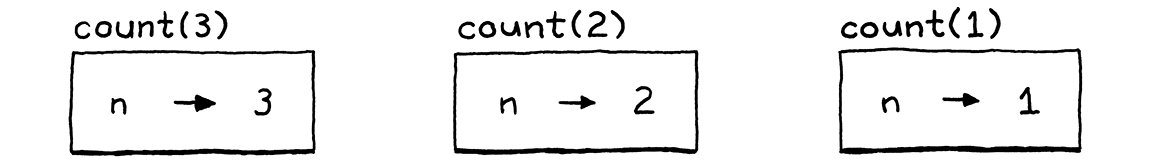
\includegraphics[width=\textwidth]{image/functions/recursion.png}
\end{figure}

这就是为什么我们在每次\textit{调用}时创建一个新的环境,而不是在函数声明时创建。我们前面看到的call()方法就是这样做的。在调用开始的时候,它创建了一个新环境。然后它以同步的方式遍历形参和实参列表。对于每一对参数,它用形参的名字创建一个新的变量,并将其与实参的值绑定。

所以,对于类似下面这样的代码:

\begin{code}{java}{}{}
fun add(a, b, c) {
  print a + b + c;
}

add(1, 2, 3);
\end{code}

在调用add()时,解释器会创建类似下面这样的内容:

\begin{figure}[htbp]
  \centering
  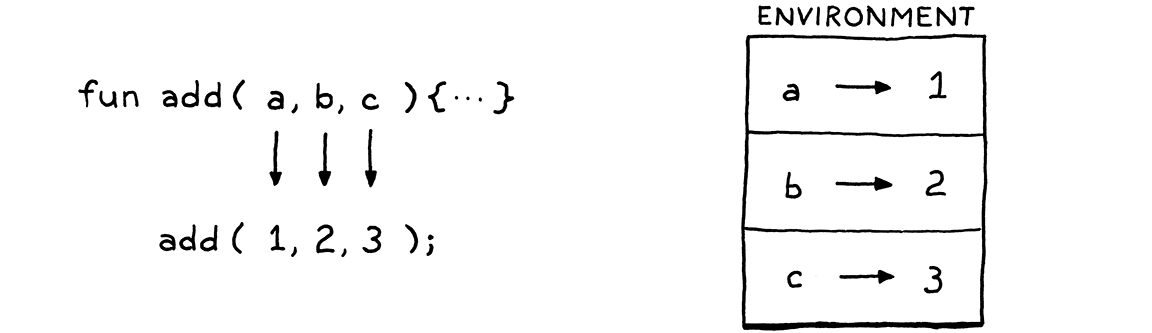
\includegraphics[width=\textwidth]{image/functions/binding.png}
\end{figure}

然后call()会告诉解释器在这个新的函数局部环境中执行函数体。在此之前,当前环境是函数被调用的位置所处的环境。现在,我们转入了为函数创建的新的参数空间中。

这就是将数据传入函数所需的全部内容。通过在执行函数主体时使用不同的环境,用同样的代码调用相同的函数可以产生不同的结果。

一旦函数的主体执行完毕,executeBlock()就会丢弃该函数的本地环境,并恢复调用该函数前的活跃环境。最后,call()方法会返回null,它向调用者返回nil。(我们会在稍后添加返回值)

从机制上讲,这段代码是非常简单的。遍历几个列表,绑定一些新变量,调用一个方法。但这就是将代码块变成有生命力的调用执行的地方。这是我在整本书中最喜欢的片段之一。如果你愿意的话,可以花点时间好好思考一下。

完成了吗?好的。注意当我们绑定参数时,我们假设参数和参数列表具有相同的长度。这是安全的,因为visitCallExpr()在调用call()之前会检查元数。它依靠报告其元数的函数来做到这一点。

\begin{code}{java}{}{lox/LoxFunction.java,在LoxFunction()方法后添加}
  @Override
  public int arity() {
    return declaration.params.size();
  }
\end{code}

这基本就是我们的函数对象表示了。既然已经到了这一步,我们也可以实现toString()。

\begin{code}{java}{}{lox/LoxFunction.java,在LoxFunction()方法后添加}
  @Override
  public String toString() {
    return "<fn " + declaration.name.lexeme + ">";
  }
\end{code}

如果用户要打印函数的值,该方法能提供一个更漂亮的输出值。

\begin{code}{js}{}{}
fun add(a, b) {
  print a + b;
}

print add; // "<fn add>".
\end{code}

\subsection{解释函数声明}

我们很快就会回头来完善LoxFunction,但是现在已足够开始进行解释了。现在,我们可以访问函数声明节点了。

\begin{code}{java}{}{lox/Interpreter.java,在visitExpressionStmt()方法后添加}
  @Override
  public Void visitFunctionStmt(Stmt.Function stmt) {
    LoxFunction function = new LoxFunction(stmt);
    environment.define(stmt.name.lexeme, function);
    return null;
  }
\end{code}

这类似于我们介绍其它文本表达式的方式。我们会接收一个函数\textit{语法}节点——函数的编译时表示形式——然后将其转换为运行时表示形式。在这里就是一个封装了语法节点的LoxFunction实例。

函数声明与其它文本节点的不同之处在于,声明还会将结果对象绑定到一个新的变量。因此,在创建LoxFunction之后,我们在当前环境中创建一个新的绑定,并在其中保存对该函数的引用。

这样,我们就可以在Lox中定义和调用我们自己的函数。试一下:

\begin{code}{js}{}{}
fun sayHi(first, last) {
  print "Hi, " + first + " " + last + "!";
}

sayHi("Dear", "Reader");
\end{code}

我不知道你怎么想的,但对我来说,这看起来像是一种虔诚的编程语言。

\section{Return语句}

我们可以通过传递参数将数据输入函数中,但是我们没有办法将结果\textit{传出来}。如果Lox是像Ruby或Scheme那样的面向表达式的语言,那么函数体就是一个表达式,其值就隐式地作为函数的结果。但是在Lox中,函数体是一个不产生值的语句列表,所有我们需要专门的语句来发出结果。换句话说,就是return语句。我相信你已经能猜出语法了。

\begin{ebnf}
statement & \rightarrow\quad exprStmt \\
& \;\;\vert\quad forStmt \\
& \;\;\vert\quad ifStmt \\
& \;\;\vert\quad printStmt \\
& \;\;\vert\quad returnStmt \\
& \;\;\vert\quad whileStmt \\
& \;\;\vert\quad block \quad ; \\
\\
returnStmt & \rightarrow\quad \mathtt{"}return\mathtt{"} \quad expression? \quad \mathtt{"};\mathtt{"} \quad ;
\end{ebnf}

我们又得到一个statement规则下的新产生式(实际上也是最后一个)。一个return语句就是一个return关键字,后跟一个可选的表达式,并以一个分号结尾。

返回值是可选的,用以支持从一个不返回有效值的函数中提前退出。在静态类型语言中,void函数不返回值,而非void函数返回值。由于Lox是动态类型的,所以没有真正的void函数。在调用一个不包含return语句的函数时,编译器没有办法阻止你获取其结果值。

\begin{code}{js}{}{}
fun procedure() {
  print "don't return anything";
}

var result = procedure();
print result; // ?
\end{code}

这意味着每个Lox函数都要返回一些内容,即使其中根本不包含return语句。我们使用nil,这就是为什么LoxFunction的call()实现在最后返回null。同样,如果你省略了return语句中的值,我们将其视为等价于:

\begin{code}{java}{}{}
return nil;
\end{code}

在AST生成器中,添加一个新节点。

\begin{code}{java}{2}{tool/GenerateAst.java,在main()方法中添加}
      "Print      : Expr expression",
      "Return     : Token keyword, Expr value",
      "Var        : Token name, Expr initializer",
\end{code}

其中保留了return关键字标记(这样我们可以使用该标记的位置来报告错误),以及返回的值(如果有的话)。我们像解析其它语句一样来解析它,首先识别起始的关键字。

\begin{code}{java}{2}{lox/Parser.java,在statement()方法中添加}
    if (match(PRINT)) return printStatement();
    if (match(RETURN)) return returnStatement();
    if (match(WHILE)) return whileStatement();
\end{code}

分支会跳转到:

\begin{code}{java}{}{lox/Parser.java,在printStatement()方法后添加}
  private Stmt returnStatement() {
    Token keyword = previous();
    Expr value = null;
    if (!check(SEMICOLON)) {
      value = expression();
    }

    consume(SEMICOLON, "Expect ';' after return value.");
    return new Stmt.Return(keyword, value);
  }
\end{code}

在捕获先前消耗的return关键字之后,我们会寻找一个值表达式。因为很多不同的标记都可以引出一个表达式,所以很难判断是否存在返回值。相反,我们检查它是否不存在。因为分号不能作为表达式的开始,如果下一个标记是分号,我们就知道一定没有返回值。

\subsection{从函数调用中返回}

解释return语句是很棘手的。你可以从函数体中的任何位置返回,甚至是深深嵌套在其它语句中的位置。当返回语句被执行时,解释器需要完全跳出当前所在的上下文,完成函数调用,就像某种顶层的控制流结构。

举例来说,假设我们正在运行下面的代码,并且我们即将执行return语句:

\begin{code}{java}{}{}
fun count(n) {
  while (n < 100) {
    if (n == 3) return n; // <--
    print n;
    n = n + 1;
  }
}

count(1);
\end{code}

Java调用栈目前看起来大致如下所示:

\begin{code}{java}{}{}
Interpreter.visitReturnStmt()
Interpreter.visitIfStmt()
Interpreter.executeBlock()
Interpreter.visitBlockStmt()
Interpreter.visitWhileStmt()
Interpreter.executeBlock()
LoxFunction.call()
Interpreter.visitCallExpr()
\end{code}

我们需要从栈顶一直回退到call()。我不知道你怎么想,但是对我来说,这听起来很像是异常。当我们执行return语句时,我们会使用一个异常来解开解释器,经过所有函数内含语句的visit方法,一直回退到开始执行函数体的代码。

新的AST节点的visit方法如下所示:

\begin{code}{java}{}{lox/Interpreter.java,在visitPrintStmt()方法后添加}
  @Override
  public Void visitReturnStmt(Stmt.Return stmt) {
    Object value = null;
    if (stmt.value != null) value = evaluate(stmt.value);

    throw new Return(value);
  }
\end{code}

如果我们有返回值,就对其求值,否则就使用nil。然后我们取这个值并将其封装在一个自定义的异常类中,并抛出该异常。

\begin{code}{java}{}{lox/Return.java,创建新文件}
package com.craftinginterpreters.lox;

class Return extends RuntimeException {
  final Object value;

  Return(Object value) {
    super(null, null, false, false);
    this.value = value;
  }
}
\end{code}

这个类使用Java运行时异常类来封装返回值。其中那个奇怪的带有null和false的父类构造器方法,禁用了一些我们不需要的JVM机制。因为我们只是使用该异常类来控制流,而不是真正的错误处理,所以我们不需要像堆栈跟踪这样的开销。

我们希望可以一直跳出到函数调用开始的地方,也就是LoxFunction中的call()方法。

\begin{code}{java}{3-7}{lox/LoxFunction.java,在call()方法中替换1行:}
         arguments.get(i));
    }
    try {
      interpreter.executeBlock(declaration.body, environment);
    } catch (Return returnValue) {
      return returnValue.value;
    }
    return null;
\end{code}

我们将对executeBlock()的调用封装在一个try-catch块中。当捕获一个返回异常时,它会取出其中的值并将其作为call()方法的返回值。如果没有捕获任何异常,意味着函数到达了函数体的末尾,而且没有遇到return语句。在这种情况下,隐式地返回nil。

我们来试一下。我们终于有能力支持这个经典的例子——递归函数计算Fibonacci数:

\begin{code}{js}{}{}
fun fib(n) {
  if (n <= 1) return n;
  return fib(n - 2) + fib(n - 1);
}

for (var i = 0; i < 20; i = i + 1) {
  print fib(i);
}
\end{code}

这个小程序练习了我们在过去几章中实现的几乎所有语言特性,包括表达式、算术运算、分支、循环、变量、函数、函数调用、参数绑定和返回。

\section{局部函数和闭包}

我们的函数功能已经相当全面了,但是还有一个漏洞需要修补。实际上,这是一个很大的问题,我们将会在下一章中花费大部分时间来修补它,但是我们可以从这里开始。

LoxFunction中的call()实现创建了一个新的环境,并在其中绑定了函数的参数。当我向你展示这段代码时,我忽略了一个重要的问题:这个环境的父类是什么?

目前,它始终是globals,即顶级的全局环境。这样,如果一个标识符不是在函数体内部定义的,解释器可以在函数外部的全局作用域中查找它。在Fibonacci的例子中,这就是解释器如何能够在函数体中实现对fib的递归调用——fib是一个全局变量。

但请记住,在Lox中,允许在可以绑定名字的*任何地方*进行函数声明。其中包括Lox脚本的顶层,但也包括块或其他函数的内部。Lox支持在另一个函数内定义或在一个块内嵌套的\textbf{局部函数}。

考虑下面这个经典的例子:

\begin{code}{js}{}{}
fun makeCounter() {
  var i = 0;
  fun count() {
    i = i + 1;
    print i;
  }

  return count;
}

var counter = makeCounter();
counter(); // "1".
counter(); // "2".
\end{code}

这个例子中,count()使用了i,它是在该函数外部的makeCounter()声明的。makeCounter()返回对count()函数的引用,然后它的函数体就执行完成了。

同时,顶层代码调用了返回的count()函数。这就执行了count()函数的主体,它会对i赋值并读取i,尽管定义i的函数已经退出。

如果你以前从未遇到过带有嵌套函数的语言,那么这可能看起来很疯狂,但用户确实希望它能工作。唉,如果你现在运行它,当count()的函数体试图查找i时,会在对counter()的调用中得到一个未定义的变量错误,这是因为当前的环境链看起来像是这样的:

\begin{figure}[htbp]
  \centering
  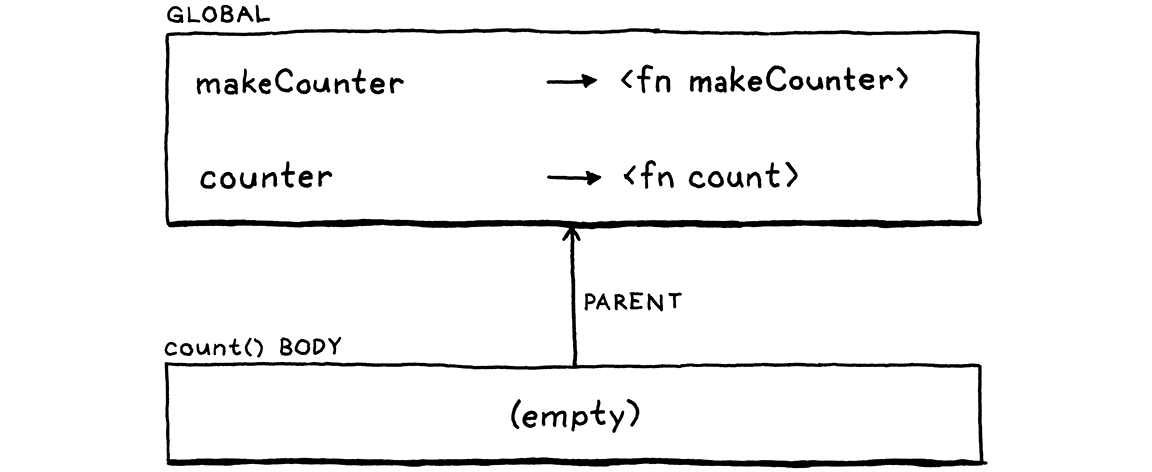
\includegraphics[width=\textwidth]{image/functions/global.png}
\end{figure}

当我们调用count()时(通过counter中保存的引用),我们会为函数体创建一个新的空环境,它的父环境就是全局环境。我们丢失了i所在的makeCounter()环境。

我们把时间往回拨一点。我们在makeCounter()的函数体中声明count()时,环境链的样子是下面这样:

\begin{figure}[htbp]
  \centering
  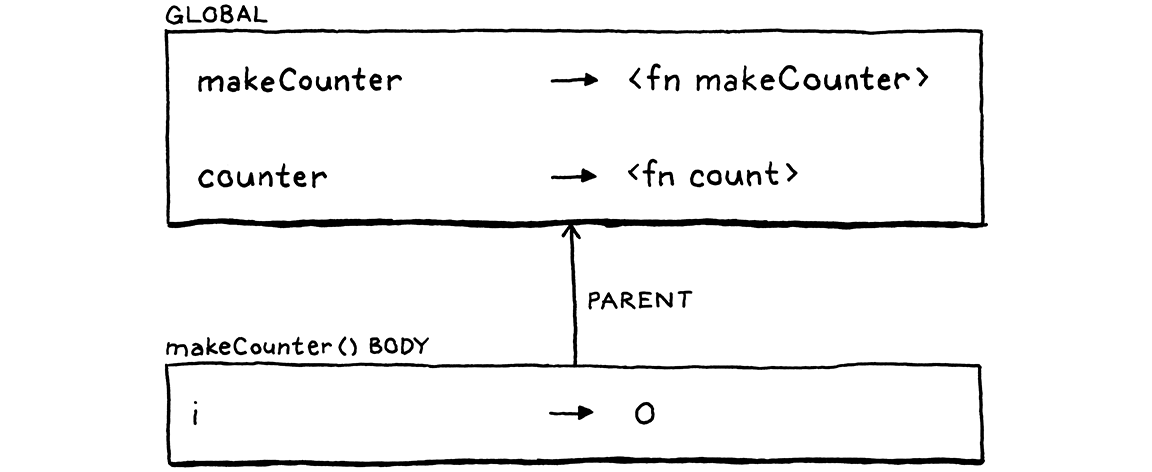
\includegraphics[width=\textwidth]{image/functions/body.png}
\end{figure}

所以,在函数声明的地方,我们可以看到i。但是当我们从makeCounter()返回并退出其主体时,解释器会丢弃这个环境。因为解释器不会保留count()外围的环境,所以要靠函数对象本身来保存它。

这种数据结构被称为\textbf{闭包},因为它“封闭”并保留着函数声明的外围变量。闭包早在Lisp时代就已经存在了,语言黑客们想出了各种方法来实现闭包。在jlox中,我们将采用最简单的方式。在LoxFunction中,我们添加一个字段来存储环境。

\begin{code}{java}{2}{lox/LoxFunction.java,在LoxFunction类中添加}
  private final Stmt.Function declaration;
  private final Environment closure;
  LoxFunction(Stmt.Function declaration) {
\end{code}

我们在构造函数中对其初始化。

\begin{code}{java}{1-2}{lox/LoxFunction.java,在LoxFunction()构造方法中替换1行:}
  LoxFunction(Stmt.Function declaration, Environment closure) {
    this.closure = closure;
    this.declaration = declaration;
\end{code}

当我们创建LoxFunction时,我们会捕获当前环境。

\begin{code}{java}{2}{lox/Interpreter.java,在visitFunctionStmt()方法中替换1行:}
    public Void visitFunctionStmt(Stmt.Function stmt) {
      LoxFunction function = new LoxFunction(stmt, environment);
      environment.define(stmt.name.lexeme, function);
\end{code}

这是函数声明时生效的环境,而不是函数被调用时的环境,这正是我们想要的。它代表了函数声明时的词法作用域。最后,当我们调用函数时,我们使用该环境作为调用的父环境,而不是直接使用globals。

\begin{code}{java}{2}{lox/LoxFunction.java,在call()方法中替换1行:}
                      List<Object> arguments) {
    Environment environment = new Environment(closure);
    for (int i = 0; i < declaration.params.size(); i++) {
\end{code}

这样就创建了一个环境链,从函数体开始,经过函数被声明的环境,然后到全局作用域。运行时环境链与源代码的文本嵌套相匹配,跟我们想要的一致。当我们调用该函数时,最终的结果是这样的:

\begin{figure}[htbp]
  \centering
  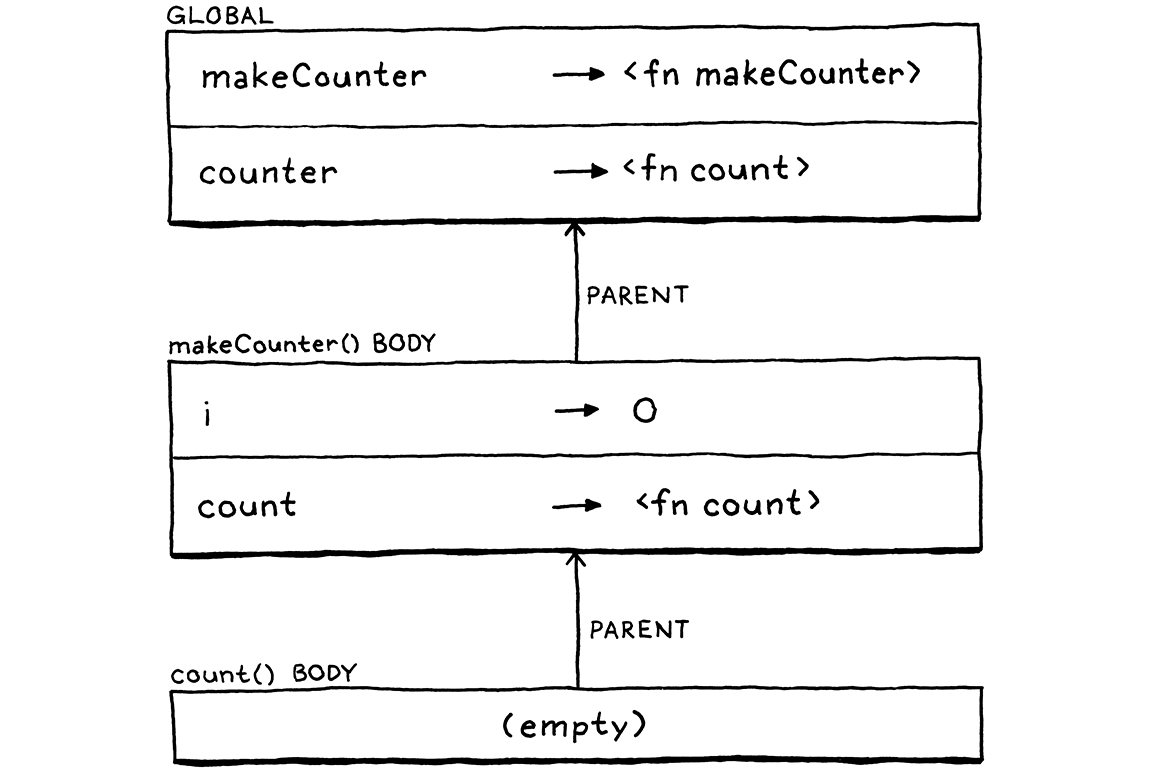
\includegraphics[width=\textwidth]{image/functions/closure.png}
\end{figure}

如你所见,现在解释器可以在需要的时候找到i,因为它在环境链中。现在尝试运行makeCounter()的例子,起作用了! 

函数让我们对代码进行抽象、重用和编排。Lox比之前的初级算术计算器要强大得多。唉,在我们匆匆忙忙支持闭包时,已经让一小部分动态作用域泄露到解释器中了。在下一章中,我们将深入探索词法作用域,堵住这个漏洞。

\section{挑战}

\begin{enumerate}
  \item 解释器会仔细检查传给函数的实参数量是否与期望的形参数量匹配。由于该检查是在运行时,针对每一次调用执行的,所以会有性能成本。Smalltalk的实现则没有这个问题。为什么呢?
  \item Lox的函数声明语法执行了两个独立的操作。它创建了一个函数,并将其与一个名称绑定。这提高了常见情况下的可用性,即你确实想把一个名字和函数联系起来。但在函数式的代码中,你经常想创建一个函数,以便立即将它传递给其他函数或返回它。在这种情况下,它不需要一个名字。

鼓励函数式风格的语言通常支持\textbf{匿名函数}或\textbf{lambdas}——一个创建函数而不用将其与名称绑定的表达式语法。在Lox中加入匿名函数的语法,已支持下面的代码:

\begin{code}{java}{}{}
fun thrice(fn) {
  for (var i = 1; i <= 3; i = i + 1) {
    fn(i);
  }
}

thrice(fun (a) {
  print a;
});
// "1".
// "2".
// "3".
\end{code}

如何处理在表达式语句中出现匿名函数表达式的棘手情况:

\begin{code}{java}{}{}
fun () {};
\end{code}

  \item 下面的代码可用吗?

\begin{code}{java}{}{}
fun scope(a) {
  var a = "local";
}
\end{code}

换句话说,一个函数的参数是跟它的局部变量在同一个作用域内,还是在一个外部作用域内?Lox 是怎么做的?你所熟悉的其他语言呢?你认为一种语言应该怎么做?
\end{enumerate}

\chapter{解析和绑定}

\epigraph{你也许偶尔会发现自己处于一种奇怪的情况。你曾以最自然的方式逐渐进入其中,但当你身处其中时,你会突然感到惊讶,并问自己这一切到底是怎么发生的。}{索尔}

哦,不! 我们的语言实现正在进水! 在我们刚添加变量和代码块时,我们把作用域控制的很好很严密。但是当我们后来添加闭包之后,我们以前防水的解释器上就出现了一个洞。大多数真正的程序都不可能从这个洞里溜走,但是作为语言实现者,我们要立下神圣的誓言,即使在语义的最深处、最潮湿的角落里也要关心正确性。

我们将用整整一章的时间来探索这个漏洞,然后小心翼翼地把它补上。在这个过程中,我们将对Lox和其他C语言传统中使用的词法范围有一个更严格的理解。我们还将有机会学习语义分析——这是一种强大的技术,用于从用户的源代码中提取语义而无需运行它。

\section{静态作用域}

快速复习一下:Lox和大多数现代语言一样,使用词法作用域。这意味着你可以通过阅读代码文本找到变量名字指向的是哪个声明。例如:

\begin{code}{java}{}{}
var a = "outer";
{
  var a = "inner";
  print a;
}
\end{code}

这里,我们知道打印的a是上一行声明的变量,而不是全局变量。运行代码并不会(也不能)影响这一点。作用域规则是语言的静态语义的一部分,这也就是为什么它们被称为静态作用域。

我还没有详细说明这些作用域规则,但是现在是时候详细说明一下了:

\textbf{变量指向的是使用变量的表达式外围环境中,前面具有相同名称的最内层作用域中的变量声明。}

其中有很多东西需要解读:

\begin{itemize}
  \item 我说的是“变量使用”而不是“变量表达式”,是为了涵盖变量表达式和赋值两种情况。类似于“使用变量的表达式”。
  \item “前面”意味着出现在\textit{程序文本}之前。

  \begin{code}{java}{}{}
  var a = "outer";
  {
    print a;
    var a = "inner";
  }
  \end{code}

  这里,打印的a是外层的,因为它在使用该变量的print语句之前。在大多数情况下,在单行代码中,文本中靠前的变量声明在时间上也先于变量使用。但并不总是如此。正如我们将看到的,函数可以推迟代码块,以使其动态执行的时间不受静态文本顺序的约束。

  \item “最内层”是因为我们的好朋友——变量遮蔽。在外围作用域中可能存在多个具有给定名称的变量。如:
  
  \begin{code}{java}{}{}
  var a = "outer";
  {
    var a = "inner";
    print a;
  }
  \end{code}
  
  我们的规则规则最内层作用域优先级最高来消除这种歧义。
\end{itemize}

由于这条规则没有提及任何运行时行为,它意味着一个变量表达式在程序的整个执行过程中总是指向同一声明。到目前为止,我们的解释器基本正确实现了这一规则。但是当我们添加了闭包后,一个错误悄悄出现了。

\begin{code}{java}{}{}
var a = "global";
{
  fun showA() {
    print a;
  }

  showA();
  var a = "block";
  showA();
}
\end{code}

在你执行这段代码之前,先思考一下它\textit{应该}输出什么。

好的...清楚了吗?如果你熟悉其它语言中的闭包,你们你可能期望会输出两次“global”。对showA()的第一次调用肯定会打印“global”,因为我们甚至还没有执行到内部变量a的声明。而根据我们的规则,一个变量表达式总数解析为同一个变量,这意味着对showA()的第二次调用也应该打印出同样的内容。

唉,它输出的是:

\begin{code}{js}{}{}
global
block
\end{code}

我要强调一下,这个代码中从未重新分配任何变量,并且只包含一个print语句。然而,不知何故,对于这个从未分配过的变量,print语句在不同的时间点上打印了两个不同的值。我们肯定在什么地方出了问题。

\subsection{作用域和可变环境}

在我们的解释器中,环境是静态作用域的动态表现。这两者大多情况下保持同步——当我们进入一个新的作用域时,我们会创建一个新的环境,当我们离开这个作用域时,我们会丢弃它。在环境中还有一个可执行的操作:在环境中绑定一个变量。这就是我们的问题所在。

让我们通过这个有问题的例子,看看每一步的环境是什么样的。首先,我们在全局作用域内声明a。

\begin{figure}[htbp]
  \centering
  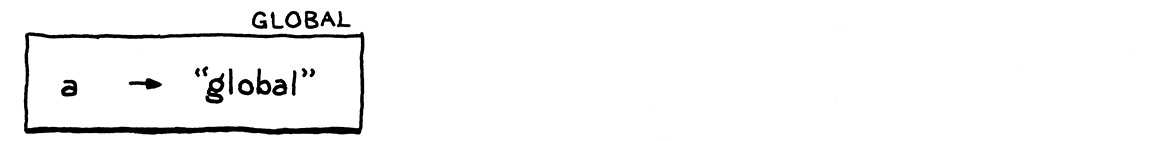
\includegraphics[width=\textwidth]{image/resolving-and-binding/environment-1.png}
\end{figure}

这为我们提供了一个环境,其中只有一个变量。然后我们进入代码块,并执行showA()的声明。

\begin{figure}[htbp]
  \centering
  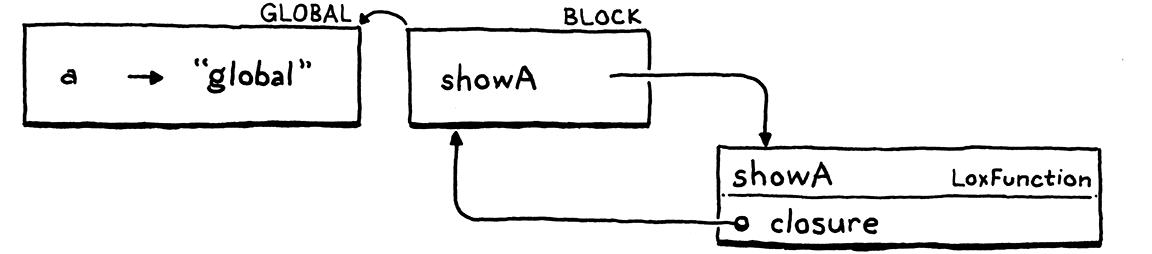
\includegraphics[width=\textwidth]{image/resolving-and-binding/environment-2.png}
\end{figure}

我们得到一个对应该代码块的新环境。在这个环境中,我们声明了一个名称showA,它绑定到为表示函数而创建的LoxFunction对象。该对象中有一个closure字段,用于捕获函数声明时的环境,因此它有一个指向该代码块环境的引用。

现在我们调用showA()。

\begin{figure}[htbp]
  \centering
  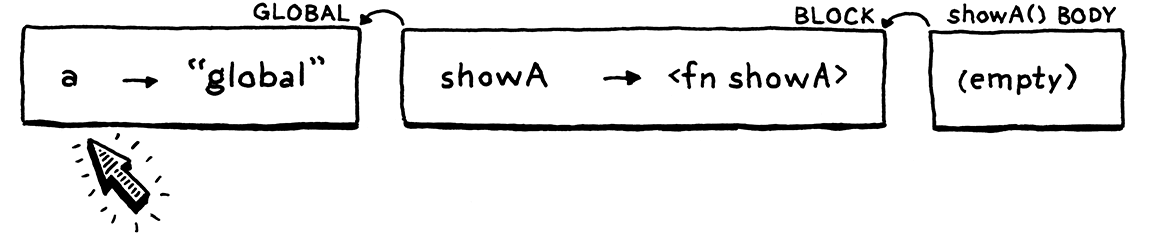
\includegraphics[width=\textwidth]{image/resolving-and-binding/environment-3.png}
\end{figure}

解释器为showA()的函数体动态地创建了一个新环境。它是空的,因为该函数没有声明任何变量。该环境的父环境是该函数的闭包——外部的代码块环境。

在showA()函数体中,输出a的值。解释器通过遍历环境链来查找这个值。它会一直到达全局环境,在其中找到变量a并打印“global”。太好了。

接下来,我们声明第二个a,这次是在代码块内。

\begin{figure}[htbp]
  \centering
  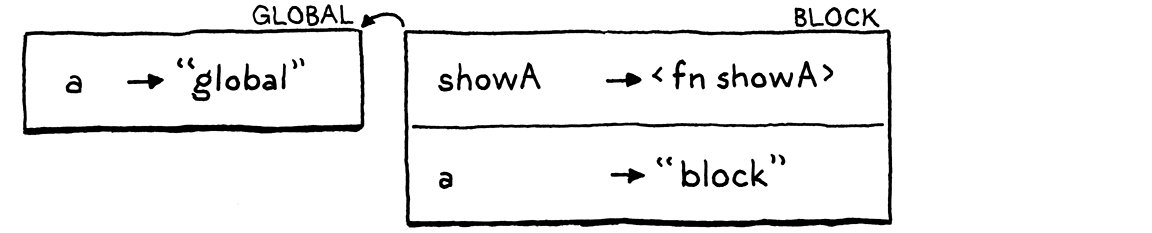
\includegraphics[width=\textwidth]{image/resolving-and-binding/environment-4.png}
\end{figure}

它和showA()在同一个代码块中——同一个作用域,所以它进入了同一个环境,也就是showA()的闭包所指向的环境。这就是有趣的地方了。我们再次调用showA()。

\begin{figure}[htbp]
  \centering
  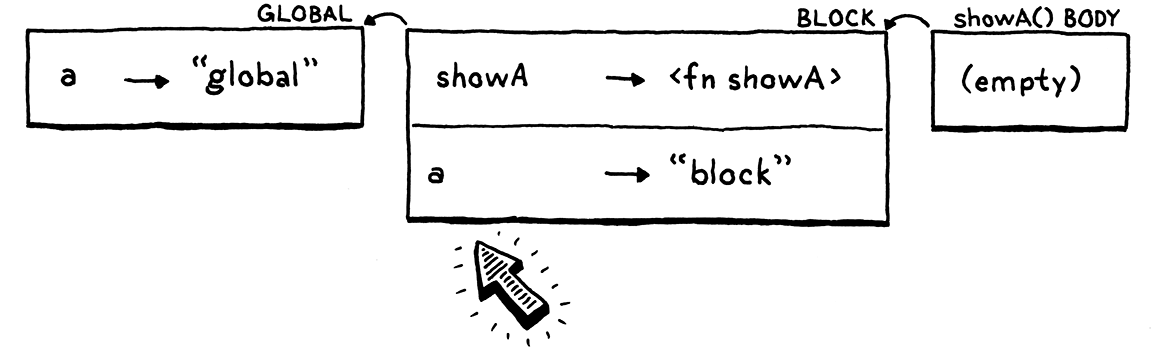
\includegraphics[width=\textwidth]{image/resolving-and-binding/environment-5.png}
\end{figure}

我们再次为showA()的函数体创建了一个新的空环境,将其连接到该闭包,并运行函数体。当解释器遍历环境链去查找a时,它会发现代码块环境中新的变量a。

我选择了一种实现环境的方式,希望它能够与您对作用域的非正式直觉相一致。我们倾向于认为一个块中的所有代码在同一个作用域中,所以我们的解释器使用了一个环境来表示它。每个环境都是一个可变的hash表。当一个新的局部变量被声明时,它会被加入该作用域的现有环境中。

就像生活中的很多直觉一样,这种直觉并不完全正确。一个代码块并不一定都是同一个作用域。考虑一下:

\begin{code}{js}{}{}
{
  var a;
  // 1.
  var b;
  // 2.
}
\end{code}

在标记的第一行,作用域中只有a。在第二行时,a和b都在其中。如果将作用域定义为一组声明,那么它们显然不是相同的作用域——它们不包含相同的声明。这就好像是var语句将代码块分割成了两个独立的作用域,变量声明前的作用域和包含新变量的作用域。

但是在我们的实现中,环境确实表现得像整个代码块是一个作用域,只是这个作用域会随时间变化。而闭包不是这样的。当函数被声明时,它会捕获一个指向当前环境的引用。函数\textit{应该}捕获一个冻结的环境快照,就像它存在于函数被声明的那一瞬间。但是事实上,在Java代码中,它引用的是一个实际可变的环境对象。当后续在该环境所对应的作用域内声明一个变量时,闭包会看到该变量,即使变量声明\textit{没有}出现在函数之前。

\subsection{持久环境}

有一种编程风格,使用所谓的\textbf{持久性数据结构}。与你在命令式编程中所熟悉的模糊的数据结构不同,持久化数据结构永远不能被直接修改。相应地,对现有结构的任何“修改”都会产生一个全新的对象,其中包含所有的原始数据和新的修改。而原有的对象则保持不变。

如果我们将这一技术应用于环境,那么每次你声明一个变量时,都会返回一个新的环境,其中包含所有先前声明的变量和一个新名称。声明一个变量会执行隐式分割,在声明变量之前与之后都有一个环境:

\begin{figure}[htbp]
  \centering
  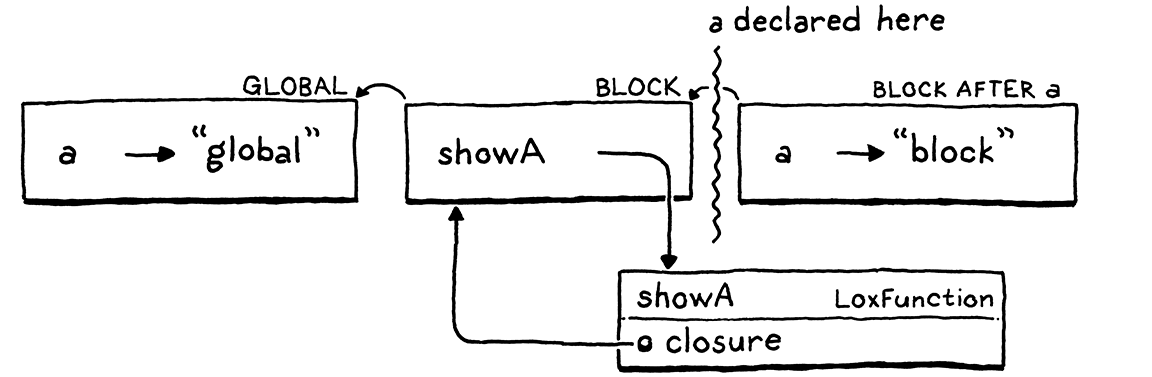
\includegraphics[width=\textwidth]{image/resolving-and-binding/split.png}
\end{figure}

当函数被声明时,闭包保留对正在运行的Environment实例的引用。由于该代码块中后续的任何声明都会生成新的Environment对象,闭包就不会看到新的变量,我们的问题也得到修复。

这是解决该问题的合法方式,也是在Scheme解释器中实现变量环境的经典方式。对于Lox,我们可以这样做,但是这意味着要回头修改一大堆现有的代码。

我不会把你拖下水的。我们将保持表示环境的方式不变。我们不会让数据变得更加静态结构化,而是将静态解析嵌入访问操作本身。

\section{语义分析}

我们的解释器每次对变量表达式求值时,都会\textbf{解析}变量——追踪它所指向的声明。如果这个变量被包在一个运行1000次的循环中,那么该变量就会被重复解析1000次。

我们知道静态作用域意味着一个变量的使用总是解析到同一个声明,而且可以通过查看文本来确定。既然如此,我们为什么每次都要动态地解析呢?这样做不仅仅导致了这个恼人的bug,而且也造成了不必要的低效。

一个更好的解决方案是一次性解析每个变量的使用。编写一段代码,检查用户的程序,找到所提到的每个变量,并找出每个变量引用的是哪个声明。这个过程是\textbf{语义分析}的一个例子。解析器只告诉程序在语法上是否正确(语法分析),而语义分析则更进一步,开始弄清楚程序的各个部分的实际含义。在这种情况下,我们的分析将解决变量绑定的问题。我们不仅要知道一个表达式是一个变量,还要知道它是哪个变量。

有很多方法可以存储变量及其声明直接的绑定关系。当我们使用Lox的C解释器时,我们将有一种更有效的方式来存储和访问局部变量。但是对于jlox来说,我想尽量减少对现有代码库的附带损害。我不希望扔掉一堆基本上都很好的代码。

相对地,我们将以最充分利用现有Environment类的方式来存储解析结果。回想一下,在有问题的例子中,a的访问是如何被解释的。

\begin{figure}[htbp]
  \centering
  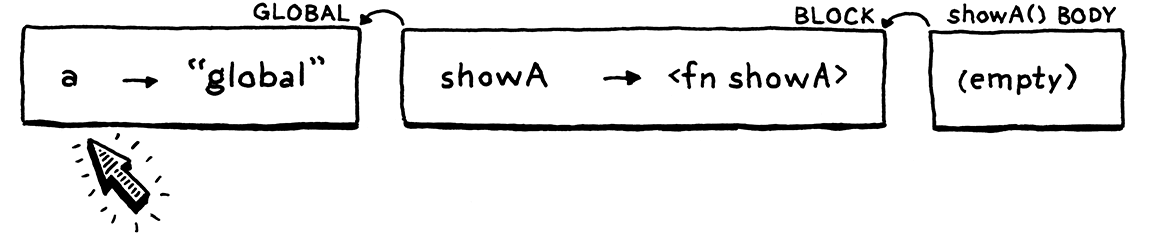
\includegraphics[width=\textwidth]{image/resolving-and-binding/environment-3.png}
\end{figure}

在第一次(正确的)求值中,我们会检查链中的环境,并找到a的全局声明。然后,当内部的a在块作用域中声明时,它会遮蔽全局的变量a。

\begin{figure}[htbp]
  \centering
  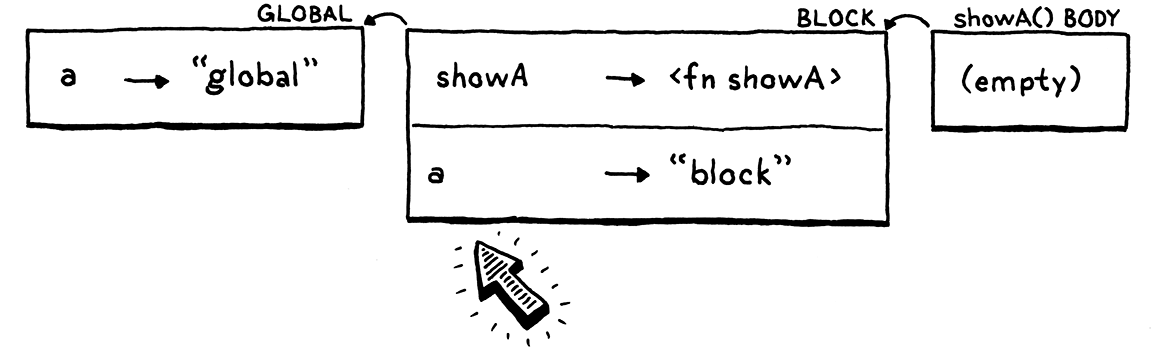
\includegraphics[width=\textwidth]{image/resolving-and-binding/environment-5.png}
\end{figure}

下一次查找会遍历环境链,在第二个环境中找到a并停止。每个环境都对应于一个声明变量的词法作用域。如果我们能够保证变量查找总是在环境链上遍历相同数量的链接,也就可以保证每次都可以在相同的作用域中找到相同的变量。

要“解析”一个变量使用,我们只需要计算声明的变量在环境链中有多少“跳”。有趣的问题是在什么时候进行这个计算——或者换句话说,在解释器的实现中,这段代码要添加到什么地方?

因为我们是根据源代码的结构来计算一个静态属性,所以答案显然是在解析器中。那是传统的选择,也是我们以后在clox中实现它的地方。在这里同样也适用,但是我想给你展示另一种技巧。我们会单独写一个解析器。

\subsection{变量解析过程}

在解析器生成语法树之后,解释器执行语法树之前,我们会对语法树再进行一次遍历,以解析其中包含的变量。在解析和执行之间的额外遍历是很常见的。如果Lox中有静态类型,我们可以插入一个类型检查器。优化也经常是在类似单独的遍历过程中实现的。基本上,任何不依赖与运行时状态的工作都可以通过这种方式完成。

我们的变量解析工作就像一个小型的解释器。它会遍历整棵树,访问每个节点,但是静态分析与动态执行还是不同的:

\begin{itemize}
  \item \textbf{没有副作用}。当静态分析处理一个print语句时,它并不会打印任何东西。对本地函数或其它与外部世界联系的操作也会被终止,并且没有任何影响。
  \item \textbf{没有控制流}。循环只会被处理一次,if语句中的两个分支都会处理,逻辑操作符也不会做短路处理。
\end{itemize}

\section{Resolver类}

与Java中的所有内容一样,我们将变量解析处理也放在一个类中。

\begin{code}{java}{}{lox/Resolver.java,创建新文件:}
package com.craftinginterpreters.lox;

import java.util.HashMap;
import java.util.List;
import java.util.Map;
import java.util.Stack;

class Resolver implements Expr.Visitor<Void>, Stmt.Visitor<Void> {
  private final Interpreter interpreter;

  Resolver(Interpreter interpreter) {
    this.interpreter = interpreter;
  }
}
\end{code}

因为解析器需要处理语法树中的每个节点,所以它实现了我们已有的访问者抽象。在解析变量时,有几个节点是比较特殊的:

\begin{itemize}
  \item 块语句为它所包含的语句引入了一个新的作用域。
  \item 函数声明为其函数体引入了一个新的作用域,并在该作用域中绑定了它的形参。
  \item 变量声明将一个新变量加入到当前作用域中。
  \item 变量定义和赋值表达式需要解析它们的变量值。
\end{itemize}

其余的节点不做任何特别的事情,但是我们仍然需要为它们实现visit方法,以遍历其子树。尽管+表达式本身没有任何变量需要解析,但是它的任一操作数都可能需要。

\subsection{解析代码块}

我们从块语法开始,因为它们创建了局部作用域——魔法出现的地方。

\begin{code}{java}{}{lox/Resolver.java,在Resolver()方法后添加}
  @Override
  public Void visitBlockStmt(Stmt.Block stmt) {
    beginScope();
    resolve(stmt.statements);
    endScope();
    return null;
  }
\end{code}

这里会开始一个新的作用域,遍历块中的语句,然后丢弃该作用域。有趣的部分都在这些辅助方法中。我们先看一个简单的。

\begin{code}{java}{}{lox/Resolver.java,在Resolver()方法后添加}
  void resolve(List<Stmt> statements) {
    for (Stmt statement : statements) {
      resolve(statement);
    }
  }
\end{code}

它会遍历语句列表,并解析其中每一条语句。它会进一步调用:

\begin{code}{java}{}{lox/Resolver.java,在visitBlockStmt()方法后添加}
  private void resolve(Stmt stmt) {
    stmt.accept(this);
  }
\end{code}

在此过程中,让我们添加一个后续解析表达式时会用到的重载方法。

\begin{code}{java}{}{lox/Resolver.java,在resolve(Stmt stmt)方法后添加}
  private void resolve(Expr expr) {
    expr.accept(this);
  }
\end{code}

这些方法与解释器中的evaluate()和execute()方法类似——它们会反过来将访问者模式应用到语法树节点。

真正有趣的部分是围绕作用域的。一个新的块作用域是这样创建的:

\begin{code}{java}{}{lox/Resolver.java,在resolve()方法后添加}
  private void beginScope() {
    scopes.push(new HashMap<String, Boolean>());
  }
\end{code}

词法作用域在解释器和解析器中都有使用。它们的行为像一个栈。解释器是使用链表(Environment对象组成的链)来实现栈的,在解析器中,我们使用一个真正的Java Stack。

\begin{code}{java}{2}{lox/Resolver.java,在Resolver类中添加}
  private final Interpreter interpreter;
  private final Stack<Map<String, Boolean>> scopes = new Stack<>();
  Resolver(Interpreter interpreter) {
\end{code}

这个字段会记录当前作用域内的栈。栈中的每个元素是代表一个块作用域的Map。与Environment中一样,键是变量名。值是布尔值,原因我很快会解释。

作用域栈只用于局部块作用域。解析器不会跟踪在全局作用域的顶层声明的变量,因为它们在Lox中是更动态的。当解析一个变量时,如果我们在本地作用域栈中找不到它,我们就认为它一定是全局的。

由于作用域被存储在一个显式的栈中,退出作用域很简单。

\begin{code}{java}{}{lox/Resolver.java,在beginScope()方法后添加}
  private void endScope() {
    scopes.pop();
  }
\end{code}

现在我们可以在一个栈中压入和弹出一个空作用域,接下来我们往里面放些内容。

\subsection{解析变量声明}

解析一个变量声明,会在当前最内层的作用域map中添加一个新的条目。这看起来很简单,但是我们需要做一些小动作。

\begin{code}{java}{}{lox/Resolver.java,在visitBlockStmt()方法后添加}
  @Override
  public Void visitVarStmt(Stmt.Var stmt) {
    declare(stmt.name);
    if (stmt.initializer != null) {
      resolve(stmt.initializer);
    }
    define(stmt.name);
    return null;
  }
\end{code}

我们将绑定分为两个步骤,先声明,然后定义,以便处理类似下面这样的边界情况:

\begin{code}{js}{}{}
var a = "outer";
{
  var a = a;
}
\end{code}

当局部变量的初始化式指向一个与当前声明变量名称相同的变量时,会发生什么?我们有几个选择:

\begin{enumerate}
  \item \textbf{运行初始化式,然后将新的变量放入作用域中}。在这个例子中,新的局部变量a会使用“outer”(全局变量a的值)初始化。换句话说,前面的声明脱糖后如下:

   \begin{code}{js}{}{}
   var temp = a; // Run the initializer.
   var a;        // Declare the variable.
   a = temp;     // Initialize it.
   \end{code}

  \item \textbf{将新的变量放入作用域中,然后运行初始化式。}这意味着你可以在变量被初始化之前观察到它,所以我们需要计算出它的值。可能是nil。这意味着新的局部变量a将被重新初始化为它自己的隐式初始化值nil。现在,脱糖后的结果如下:

   \begin{code}{js}{}{}
   var a; // Define the variable.
   a = a; // Run the initializer.
   \end{code}

  \item \textbf{在初始化式中引用一个变量是错误的。}如果初始化式使用了要初始化的变量,则解释器在编译时或运行时都会失败。
\end{enumerate}

前两个选项中是否有用户真正\textit{想要}的?变量遮蔽很少见,而且通常是一个错误,所以根据被遮蔽的变量值来初始化一个遮蔽的变量,似乎不太可能是有意为之。

第二个选项就更没用了。新变量的值总是nil。通过名称来引用没有任何意义。你可以使用一个隐式的nil来代替。

由于前两个选项可能会掩盖用户的错误,我们将采用第三个选项。此外,我们要将其作为一个编译错误而不是运行时错误。这样一来,在代码运行之前,用户就会收到该问题的警报。

要做到这一点,当我们访问表达式时,我们需要知道当前是否在某个变量的初始化式中。我们通过将绑定拆分为两步来实现。首先是\textbf{声明}。

\begin{code}{java}{}{lox/Resolver.java,在endScope()方法后添加}
  private void declare(Token name) {
    if (scopes.isEmpty()) return;

    Map<String, Boolean> scope = scopes.peek();
    scope.put(name.lexeme, false);
  }
\end{code}

声明将变量添加到最内层的作用域,这样它就会遮蔽任何外层作用域,我们也就知道了这个变量的存在。我们通过在作用域map中将其名称绑定到false来表明该变量“尚未就绪”。作用域map中与key相关联的值代表的是我们是否已经结束了对变量初始化式的解析。

在声明完变量后,我们在变量当前存在但是不可用的作用域中解析变量的初始化表达式。一旦初始化表达式完成,变量也就绪了。我们通过\textbf{define}来实现。

\begin{code}{java}{}{lox/Resolver.java,在declare()方法后添加}
  private void define(Token name) {
    if (scopes.isEmpty()) return;
    scopes.peek().put(name.lexeme, true);
  }
\end{code}

我们在作用域map中将变量的值置为true,以标记它已完全初始化并可使用。它有了生命!

\subsection{解析变量表达式}

变量声明——以及我们即将讨论的函数声明——会向作用域map中写数据。在我们解析变量表达式时,需要读取这些map。

\begin{code}{java}{}{lox/Resolver.java,在visitVarStmt()方法后添加}
  @Override
  public Void visitVariableExpr(Expr.Variable expr) {
    if (!scopes.isEmpty() &&
        scopes.peek().get(expr.name.lexeme) == Boolean.FALSE) {
      Lox.error(expr.name,
          "Can't read local variable in its own initializer.");
    }

    resolveLocal(expr, expr.name);
    return null;
  }
\end{code}

首先,我们要检查变量是否在其自身的初始化式中被访问。这也就是作用域map中的值发挥作用的地方。如果当前作用域中存在该变量,但是它的值是false,意味着我们已经声明了它,但是还没有定义它。我们会报告一个错误出来。

在检查之后,我们实际上使用了这个辅助方法来解析变量:

\begin{code}{java}{}{lox/Resolver.java,在define()方法后添加}
  private void resolveLocal(Expr expr, Token name) {
    for (int i = scopes.size() - 1; i >= 0; i--) {
      if (scopes.get(i).containsKey(name.lexeme)) {
        interpreter.resolve(expr, scopes.size() - 1 - i);
        return;
      }
    }
  }
\end{code}

这看起来很像是Environment中对变量求值的代码。我们从最内层的作用域开始,向外扩展,在每个map中寻找一个可以匹配的名称。如果我们找到了这个变量,我们就对其解析,传入当前最内层作用域和变量所在作用域之间的作用域的数量。所以,如果变量在当前作用域中找到该变量,则传入0;如果在紧邻的外网作用域中找到,则传1。明白了吧。

如果我们遍历了所有的作用域也没有找到这个变量,我们就不解析它,并假定它是一个全局变量。稍后我们将讨论resolve()方法的实现。现在,让我们继续浏览其他语法节点。

\subsection{解析赋值表达式}

另一个引用变量的表达式就是赋值表达式。解析方法如下:

\begin{code}{java}{}{lox/Resolver.java,在visitVarStmt()方法后添加}
  @Override
  public Void visitAssignExpr(Expr.Assign expr) {
    resolve(expr.value);
    resolveLocal(expr, expr.name);
    return null;
  }
\end{code}

首先,我们解析右值的表达式,以防它还包含对其它变量的引用。然后使用现有的resolveLocal()方法解析待赋值的变量。

\subsection{解析函数声明}

最后是函数。函数既绑定名称又引入了作用域。函数本身的名称被绑定在函数声明时所在的作用域中。当我们进入函数体时,我们还需要将其参数绑定到函数内部作用域中。

\begin{code}{java}{}{lox/Resolver.java,在visitBlockStmt()方法后添加}
  @Override
  public Void visitFunctionStmt(Stmt.Function stmt) {
    declare(stmt.name);
    define(stmt.name);

    resolveFunction(stmt);
    return null;
  }
\end{code}

与visitVariableStmt()类似,我们在当前作用域中声明并定义函数的名称。与变量不同的是,我们在解析函数体之前,就急切地定义了这个名称。这样函数就可以在自己的函数体中递归地使用自身。

那么我们可以使用下面的方法来解析函数体:

\begin{code}{java}{}{lox/Resolver.java,在resolve()方法后添加}
  private void resolveFunction(Stmt.Function function) {
    beginScope();
    for (Token param : function.params) {
      declare(param);
      define(param);
    }
    resolve(function.body);
    endScope();
  }
\end{code}

这是一个单独的方法,因为我们以后添加类时,还需要使用它来解析Lox方法。它为函数体创建一个新的作用域,然后为函数的每个参数绑定变量。

一旦就绪,它就会在这个作用域中解析函数体。这与解释器处理函数声明的方式不同。在\textit{运行时},声明一个函数不会对函数体做任何处理。直到后续函数被调用时,才会触及主体。在\textit{静态}分析中,我们会立即遍历函数体。

\subsection{解析其它语法树节点}

这涵盖了语法中很多有趣的部分。我们处理了声明、读取、写入遍历,创建、销毁作用域的部分。虽然其它部分不受遍历解析的影响,我们也需要为其它语法树节点提供visit方法,以便递归到它们的子树。抱歉,这部分内容很枯燥,但请耐心听我讲。我们采用“自上而下”的方式,从语句开始。

一个表达式语句中包含一个需要遍历的表达式。

\begin{code}{java}{}{lox/Resolver.java,在visitBlockStmt()方法后添加}
  @Override
  public Void visitExpressionStmt(Stmt.Expression stmt) {
    resolve(stmt.expression);
    return null;
  }
\end{code}

if语句包含一个条件表达式,以及一个或两个分支语句。

\begin{code}{java}{}{lox/Resolver.java,在visitFunctionStmt()方法后添加}
  @Override
  public Void visitIfStmt(Stmt.If stmt) {
    resolve(stmt.condition);
    resolve(stmt.thenBranch);
    if (stmt.elseBranch != null) resolve(stmt.elseBranch);
    return null;
  }
\end{code}

在这里,我们可以看到解析与解释是不同的。当我们解析if语句时,没有控制流。我们会解析条件表达式和两个分支表达式。动态执行则只会进入\textit{正在执行}的分支,而静态分析是保守的——它会分析所有\textit{可能执行}的分支。因为任何一个分支在运行时都可能被触及,所以我们要对两者都进行解析。

与表达式语句类似,print语句也包含一个子表达式。

\begin{code}{java}{}{lox/Resolver.java,在visitIfStmt()方法后添加}
  @Override
  public Void visitPrintStmt(Stmt.Print stmt) {
    resolve(stmt.expression);
    return null;
  }
\end{code}

return语句也是相同的。

\begin{code}{java}{}{lox/Resolver.java,在visitPrintStmt()方法后添加}
  @Override
  public Void visitReturnStmt(Stmt.Return stmt) {
    if (stmt.value != null) {
      resolve(stmt.value);
    }

    return null;
  }
\end{code}

与if语句一样,对于while语句,我们会解析其条件,并解析一次循环体。

\begin{code}{java}{}{lox/Resolver.java,在visitVarStmt()方法后添加}
  @Override
  public Void visitWhileStmt(Stmt.While stmt) {
    resolve(stmt.condition);
    resolve(stmt.body);
    return null;
  }
\end{code}

这样就涵盖了所有的语句。接下来是表达式...

我们的老朋友二元表达式。我们要遍历并解析两个操作数。

\begin{code}{java}{}{lox/Resolver.java,在visitAssignExpr()方法后添加}
  @Override
  public Void visitBinaryExpr(Expr.Binary expr) {
    resolve(expr.left);
    resolve(expr.right);
    return null;
  }
\end{code}

调用也是类似的——我们遍历参数列表并解析它们。被调用的对象也是一个表达式(通常是一个变量表达式),所以它也会被解析。

\begin{code}{java}{}{lox/Resolver.java,在visitBinaryExpr()方法后添加}
  @Override
  public Void visitCallExpr(Expr.Call expr) {
    resolve(expr.callee);

    for (Expr argument : expr.arguments) {
      resolve(argument);
    }

    return null;
  }
\end{code}

括号表达式比较简单。

\begin{code}{java}{}{lox/Resolver.java,在visitCallExpr()方法后添加}
  @Override
  public Void visitGroupingExpr(Expr.Grouping expr) {
    resolve(expr.expression);
    return null;
  }
\end{code}

字面量表达式是最简单的。

\begin{code}{java}{}{lox/Resolver.java,在visitGroupingExpr()方法后添加}
  @Override
  public Void visitLiteralExpr(Expr.Literal expr) {
    return null;
  }
\end{code}

字面表达式中没有使用任何变量,也不包含任何子表达式,所以也不需要做任何事情。

因为静态分析没有控制流或短路处理,逻辑表达式与其它的二元运算符是一样的。

\begin{code}{java}{}{lox/Resolver.java,在visitLiteralExpr()方法后添加}
  @Override
  public Void visitLogicalExpr(Expr.Logical expr) {
    resolve(expr.left);
    resolve(expr.right);
    return null;
  }
\end{code}

接下来是最后一个节点,我们解析它的一个操作数。

\begin{code}{java}{}{lox/Resolver.java,在visitLogicalExpr()方法后添加}
  @Override
  public Void visitUnaryExpr(Expr.Unary expr) {
    resolve(expr.right);
    return null;
  }
\end{code}

有了这些visit方法,Java编译器应该会认为Resolver完全实现了Stmt.Visitor和Expr.Visitor。现在是时候休息一下了。

\section{解释已解析的变量}

让我们看看解析器有什么用处。每次访问一个变量时,它都会告诉解释器,在当前作用域和变量定义的作用域之间隔着多少层作用域。在运行时,这正好对应于当前环境与解释器可以找到变量值的外围环境之间的\textit{environments}数量。解析器通过调用下面的方法将这个数字传递给解释器:

\begin{code}{java}{}{lox/Interpreter.java,在execute()方法后添加}
  void resolve(Expr expr, int depth) {
    locals.put(expr, depth);
  }
\end{code}

我们要把解析信息存储在某个地方,这样在执行变量表达式和赋值表达式时就可以使用它,但是要存在哪里呢?一个明显的位置就是语法树节点本身。这是一个很好的方法,许多编译器都是在这里存储类似的分析结果的。

我们可以这样做,但是需要对我们的语法树生成器进行修改。相反,我们会采用另一种常见的方法,将其存储在一个map中,将每个语法树节点与其解析的数据关联起来。

像IDE这种的交互式工具经常会增量地对用户的部分代码进行重新分析和解析。当这些状态隐藏在语法树的枝叶中时,可能很难找到所有需要重新计算的状态。将这些数据存储在节点之外的好处之一就是,可以很容易地丢弃这部分数据——只需要清除map即可。

\begin{code}{java}{2}{lox/Interpreter.java,在Interpreter类中添加}
  private Environment environment = globals;
  private final Map<Expr, Integer> locals = new HashMap<>();
  Interpreter() {
\end{code}

你可能认为我们需要某种嵌套的树状结构,以避免在有多个表达式引用同一个变量时出现混乱,但是每个表达式节点都有其对应的Java对象,具有唯一性标识。一个简单的map就足以将它们全部区分开来。

与之前一样,使用集合需要先引入一些包名称。

\begin{code}{java}{2}{lox/Interpreter.java,添加}
import java.util.ArrayList;
import java.util.HashMap;
import java.util.List;
\end{code}

还有:

\begin{code}{java}{2}{lox/Interpreter.java,添加}
import java.util.List;
import java.util.Map;
class Interpreter implements Expr.Visitor<Object>,
\end{code}

\subsection{访问已解析的变量}

我们的解释器现在可以访问每个变量的解析位置。最后,我们可以利用这一点了,将变量表达式的visit方法替换如下:

\begin{code}{java}{2}{lox/Interpreter.java,在visitVariableExpr()方法中替换1行:}
  public Object visitVariableExpr(Expr.Variable expr) {
    return lookUpVariable(expr.name, expr);
  }
\end{code}

这里引用了:

\begin{code}{java}{}{lox/Interpreter.java,在visitVariableExpr()方法后添加}
  private Object lookUpVariable(Token name, Expr expr) {
    Integer distance = locals.get(expr);
    if (distance != null) {
      return environment.getAt(distance, name.lexeme);
    } else {
      return globals.get(name);
    }
  }
\end{code}

这里有几件事要做。首先,我们在map中查找已解析的距离值。要记住,我们只解析了本地变量。全局变量被特殊处理了,不会出现了map中(所以它的名字叫locals)。所以,如果我们没有在map中找到变量对应的距离值,它一定是全局变量。在这种情况下,我们直接在全局environment中查找。如果变量没有被定义,就会产生一个运行时错误。

如果我们\textit{确实}查到了一个距离值,那这就是个局部变量,我们可以利用静态分析的结果。我们不会调用get()方法,而是调用下面这个Environment中的新方法:

\begin{code}{java}{}{lox/Environment.java,在define()方法后添加}
  Object getAt(int distance, String name) {
    return ancestor(distance).values.get(name);
  }
\end{code}

原先的get()方法会动态遍历外围的环境链,搜索每一个环境,查看变量是否包含在其中。但是现在我们明确知道链路中的哪个环境中会包含该变量。我们使用下面的辅助方法直达这个环境:

\begin{code}{java}{}{lox/Environment.java,在define()方法后添加}
  Environment ancestor(int distance) {
    Environment environment = this;
    for (int i = 0; i < distance; i++) {
      environment = environment.enclosing; 
    }

    return environment;
  }
\end{code}

该方法在环境链中经过确定的跳数之后,返回对应的环境。一旦我们有了环境,getAt()方法就可以直接返回对应环境map中的变量值。甚至不需要检查变量是否存在——我们知道它是存在的,因为解析器之前已经确认过了。

\subsection{赋值已解析的变量}

我们也可以通过赋值来使用一个变量。赋值表达式对应的visit方法的修改也是类似的。

\begin{code}{java}{3-8}{lox/Interpreter.java,在visitAssignExpr()方法中替换1行:}
  public Object visitAssignExpr(Expr.Assign expr) {
    Object value = evaluate(expr.value);  
    Integer distance = locals.get(expr);
    if (distance != null) {
      environment.assignAt(distance, expr.name, value);
    } else {
      globals.assign(expr.name, value);
    }
    return value;
\end{code}

又一次,我们要查找变量的作用域距离。如果没有找到,我们就假定它是全局变量并采用跟之前一样的方式来处理;否则,我们使用下面的新方法:

\begin{code}{java}{}{lox/Environment.java,在getAt()方法后添加}
  void assignAt(int distance, Token name, Object value) {
    ancestor(distance).values.put(name.lexeme, value);
  }
\end{code}

正如getAt()与get()的关系,assignAt()对应于assign()。它会遍历固定数量的环境,然后在其map中塞入新的值。

解释器就只需要做这些调整。这也就是为什么我为解析数据选择了一种侵入性最小的表示方法。其余所有节点都跟之前一样,甚至连修改环境的代码也没有改动。

\subsection{运行解析器}

不过,我们确实需要\textit{运行}解析器。我们在解析器完成工作之后插入一次解析器处理。

\begin{code}{java}{3-4}{lox/Lox.java,在run()方法中添加代码:}
    // Stop if there was a syntax error.
    if (hadError) return;
    Resolver resolver = new Resolver(interpreter);
    resolver.resolve(statements);
    interpreter.interpret(statements);
\end{code}

如果前面的分析中存在任何错误,我们都不会运行解析器。如果代码有语法错误,它就不会运行,所以解析它的价值不大。如果语法是干净的,我们就告诉解析器做该做的事。解析器中有一个对解释器的引用,当它遍历变量时,会将解析数据直接放入解释器中。解释器后续运行时,它就具备了所需的一切数据。

退一步讲,如果解析器成功了,这么说就是对的。但是如果解析过程中出现错误会怎么办?

\section{解析错误}

由于我们正在进行语义分析,因此我们有机会使Lox的语义更加精确,以帮助用户在执行代码之前及早发现错误。看一下下面这个坏代码:

\begin{code}{js}{}{}
fun bad() {
  var a = "first";
  var a = "second";
}
\end{code}

我们确实允许在\textit{全局}作用域内声明多个同名的变量,但在局部作用域内这样做可能是错误的。如果用户知道变量已经存在,就应该使用赋值操作而不是var。如果他们不知道变量的存在,他们可能并不想覆盖之前的变量。

我们可以在解析的时候静态地检测到这个错误。

\begin{code}{java}{2-5}{lox/Resolver.java,在declare()方法中添加}
    Map<String, Boolean> scope = scopes.peek();
    if (scope.containsKey(name.lexeme)) {
      Lox.error(name,
          "Already variable with this name in this scope.");
    }
    scope.put(name.lexeme, false);
\end{code}

当我们在局部作用域中声明一个变量时,我们已经知道了之前在同一作用域中声明的每个变量的名字。如果我们看到有冲突,我们就报告一个错误。

\subsection{无效返回错误}

这是另一个讨人厌的小脚本:

\begin{code}{java}{}{}
return "at top level";
\end{code}

这里执行了一个return语句,但它甚至根本不在函数内部。这是一个顶层代码。我不知道用户认为会发生什么,但是我认为我们不希望Lox允许这种做法。

我们可以对解析器进行扩展来静态检测这种错误。就像我们遍历语法树时跟踪作用域一样,我们也可以跟踪当前访问的代码是否在一个函数声明内部。

\begin{code}{java}{2}{lox/Resolver.java,在Resolver类中添加代码:}
  private final Stack<Map<String, Boolean>> scopes = new Stack<>();
  private FunctionType currentFunction = FunctionType.NONE;
  Resolver(Interpreter interpreter) {
\end{code}

我们不是使用一个简单的Boolean值,而是使用下面这个有趣的枚举:

\begin{code}{java}{}{lox/Resolver.java,在Resolver()方法后添加}
  private enum FunctionType {
    NONE,
    FUNCTION
  }
\end{code}

现在看来又得蠢,但是我们稍后会添加更多案例,到时候它将更有意义。当我们解析函数声明时,将其作为参数传入。

\begin{code}{java}{2}{lox/Resolver.java,在visitFunctionStmt()方法中,替换1行}
    define(stmt.name);
    resolveFunction(stmt, FunctionType.FUNCTION);
    return null;
\end{code}

在resolveFunction()中,我们接受该参数,并在解析函数体之前将其保存在字段中。

\begin{code}{java}{1-4}{lox/Resolver.java,在resolveFunction()方法中替换1行:}
	private void resolveFunction(
      Stmt.Function function, FunctionType type) {
    FunctionType enclosingFunction = currentFunction;
    currentFunction = type;
    beginScope();
\end{code}

我们先把该字段的旧值存在一个局部变量中。记住,Lox中有局部函数,所以你可以任意深度地嵌套函数声明。我们不仅需要跟踪是否在一个函数内部,还要记录我们在\textit{多少}函数内部。

我们可以使用一个显式的FunctionType值堆栈来进行记录,但我们会借助JVM的力量。我们将前一个值保存在Java堆栈中的一个局部变量。当我们完成函数体的解析之后,我们将该字段恢复为之前的值。

\begin{code}{java}{2}{lox/Resolver.java,在resolveFunction()方法中添加代码:}
    endScope();
    currentFunction = enclosingFunction;
  }
\end{code}

既然我们能知道是否在一个函数声明中,那我们就可以在解析return语句时进行检查。

\begin{code}{java}{2-4}{lox/Resolver.java,在visitReturnStmt()方法中添加代码:}
  public Void visitReturnStmt(Stmt.Return stmt) {
    if (currentFunction == FunctionType.NONE) {
      Lox.error(stmt.keyword, "Can't return from top-level code.");
    }
    if (stmt.value != null) {
\end{code}

很简洁,对吧?

还有一件事。回到将所有部分整合到一起的主类Lox中,我们很小心,如果遇到任何解析错误就不会运行解释器。这个检查是在解析器\textit{之前}运行的,这样我们就不需要再去尝试解析语法无效的代码。

但是如果在解析变量时存在错误,也需要跳过解释器,所以我们添加\textit{另一个}检查。

\begin{code}{java}{2-3}{lox/Lox.java,在run()方法中添加代码:}
    resolver.resolve(statements);
    // Stop if there was a resolution error.
    if (hadError) return;
    interpreter.interpret(statements);
\end{code}

你可以想象在这里做很多其它分析。例如,我们在Lox中添加了break语句,而我们可能想确保它只能在循环体中使用。

我们还可以更进一步,对那些不一定是错误但可能没有用的代码提出警告。举例来说,如果在return语句后有不可触及的代码,很多IDE都会发出警告,或者是一个局部变量的值从没有被使用过。所有这些都可以很简单地添加到我们的静态分析过程中,或者作为单独的分析过程。

但是,就目前而言,我们会坚持这种有限的分析。重要的是,我们修复了一个奇怪又烦人的边界情况bug,尽管花费了这么多精力可能有些令人意外。

\section{挑战}

\begin{enumerate}
  \item 为什么先定义与函数名称绑定的变量是安全的,而其它变量必须等到初始化后才能使用?
  \item 你知道其它语言中是如何处理局部变量在初始化式中引用了相同名称变量的情况?比如:

\begin{code}{js}{}{}
var a = "outer";
{
  var a = a;
}
\end{code}

这是一个运行时错误?编译错误?还是允许这种操作?它们对待全局变量的方式有区别吗?你是否认同它们的选择?证明你的答案。

  \item 对解析器进行扩展,如果局部变量没有被使用就报告一个错误。
  \item 我们的解析器会计算出变量是在哪个环境中找到的,但是它仍然需要根据名称在对应的map中查找。一个更有效的环境表示形式是将局部变量保存在一个数组中,并通过索引来查找它们。

扩展解析器,为作用域中声明的每个局部变量关联一个唯一的索引。当解析一个变量的访问时,查找变量所在的作用域及对应的索引,并保存起来。在解释器中,使用这个索引快速的访问一个变量。
\end{enumerate}

\chapter{类}

\epigraph{如果一个人没有完全了解任何事物的本质,他就没有权利去爱或恨它。伟大的爱来自于对所爱之物的深刻了解,如果你对它知之甚少,你就只能爱一点点,或者根本不爱它。}{列奥纳多·达·芬奇}

我们已经完成了11章,你机器上的解释器几乎是一个完整的脚步语言实现了。它可以使用一些内置的数据结构,如列表和map,当然还需要一个用于文件IO、用户输入等的核心库。但作为语言本身已经足够了。我们有一个与BASIC、Tcl、Scheme(不包括宏)以及早期版本的Python和Lua相同的小程序语言。

如果现在是80年代,我们就可以到此为止。但是现在,很多流行的语言都支持“面向对象编程”。在Lox中添加该功能,可以为用户提供一套熟悉的工具来编写大型程序。即使你个人不喜欢OOP,这一章和下一章将帮助你理解别人是如何设计和构建对象系统的。

\section{面向对象和类}

面向对象编程有三大途径:类、原型和多方法。类排在第一位,是最流行的风格。随着JavaScript(其次是Lua)的兴起,原型也比以前更加广为人知。稍后我们会更多地讨论这些问题。对于Lox,我们采取的是经典的方法。

既然你已经跟我一起编写了大约1000行Java代码,我假设你不需要对面向对象进行详细介绍。OOP的主要目标就是将数据与作用于数据的代码捆绑在一起。用户通过声明一个类来实现这一点:

\begin{enumerate}
  \item 公开构造器以创建和初始化该类的新实例。
  \item 提供在实例上存储和访问\textit{字段}的方法。
  \item 定义一组由类的所有实例共享的\textit{方法},这些方法对每个实例的状态进行操作。
\end{enumerate}

这大概是最低要求。大多数面向对象的语言(一直追溯到Simula),也都是通过继承来跨类重用行为。我们会在下一章中添加该功能。即使剔除了这些,我们仍然有很多东西需要完成。这是一个很大的章节,直到我们完成上述所有内容之后,才能把所有东西整合到一起。所以请集中精力。

\section{类的声明}

跟之前一样,我们从语法开始。class语句引入了一个新名称,所以它应该在declaration语法规则中。

\begin{ebnf}
declaration &\rightarrow\quad classDecl \\
&\;\;\vert\quad funDecl \\
&\;\;\vert\quad varDecl \\
&\;\;\vert\quad statement \quad ; \\
\\
classDecl &\rightarrow\quad \mathtt{"}class\mathtt{"} \quad IDENTIFIER \quad \mathtt{"}{\mathtt{"} \quad function* \quad \mathtt{"}}\mathtt{"} \quad ;
\end{ebnf}

新的classDecl规则依赖于前面定义的function规则。复习一下:

\begin{ebnf}
function   &\rightarrow\quad IDENTIFIER \quad \mathtt{"}(\mathtt{"} \quad parameters? \quad \mathtt{"})\mathtt{"} \quad block \quad ; \\
parameters &\rightarrow\quad IDENTIFIER \quad ( \quad \mathtt{"},\mathtt{"} \quad IDENTIFIER \quad )* \quad ;
\end{ebnf}

用简单的英语来说,类声明就是class关键字,后跟类的名称,然后是一对花括号包含的主体。在这个主体中,有一个方法声明的列表。与函数声明不同的是,方法没有前导的fun关键字。每个方法就是一个名称、参数列表和方法主体。下面是一个例子:

\begin{code}{java}{}{}
class Breakfast {
  cook() {
    print "Eggs a-fryin'!";
  }

  serve(who) {
    print "Enjoy your breakfast, " + who + ".";
  }
}
\end{code}

像大多数动态类型的语言一样,字段没有在类的声明中明确列出。实例是松散的数据包,你可以使用正常的命令式代码自由地向其中添加字段。

在AST生成器中,classDecl语法规则有自己的语句节点。

\begin{code}{java}{2}{tool/GenerateAst.java,在main()方法中添加}
      "Block      : List<Stmt> statements",
      "Class      : Token name, List<Stmt.Function> methods",
      "Expression : Expr expression",
\end{code}

它存储了类的名称和其主体内的方法。方法使用现有的表示函数声明的Stmt.Function类来表示。这就为我们提供了一个方法所需的所有状态:名称、参数列表和方法体。

类可以出现在任何允许名称声明的地方,由前导的class关键字来触发。

\begin{code}{java}{2-3}{lox/Parser.java,在declaration()方法中添加}
    try {
      if (match(CLASS)) return classDeclaration();
      if (match(FUN)) return function("function");
\end{code}

进一步调用:

\begin{code}{java}{}{lox/Parser.java,在declaration()方法后添加}
  private Stmt classDeclaration() {
    Token name = consume(IDENTIFIER, "Expect class name.");
    consume(LEFT_BRACE, "Expect '{' before class body.");

    List<Stmt.Function> methods = new ArrayList<>();
    while (!check(RIGHT_BRACE) && !isAtEnd()) {
      methods.add(function("method"));
    }

    consume(RIGHT_BRACE, "Expect '}' after class body.");

    return new Stmt.Class(name, methods);
  }
\end{code}

这比其它大多数解析方法都更有内容,但它大致上遵循了语法。我们已经使用了class关键字,所以我们接下来会查找预期的类名,然后是左花括号。一旦进入主体,我们就继续解析方法声明,直到碰到右花括号。每个方法声明是通过调用function()方法来解析的,我们在介绍函数的那一章中定义了该函数。

就像我们在解析器中的所有开放式循环中的操作一样,我们也要检查是否到达文件结尾。这在正确的代码是不会发生的,因为类的结尾应该有一个右花括号,但它可以确保在用户出现语法错误而忘记正确结束类的主体时,解析器不会陷入无限循环。

我们将名称和方法列表封装到Stmt.Class节点中,这样就完成了。以前,我们会直接进入解释器中,但是现在我们需要先进入分析器中对节点进行分析。

\begin{code}{java}{}{lox/Resolver.java,在visitBlockStmt()方法后添加}
  @Override
  public Void visitClassStmt(Stmt.Class stmt) {
    declare(stmt.name);
    define(stmt.name);
    return null;
  }
\end{code}

我们还不用担心针对方法本身的分析,我们目前需要做的是使用类的名称来声明这个类。将类声明为一个局部变量并不常见,但是Lox中允许这样做,所以我们需要正确处理。

现在我们解释一下类的声明。

\begin{code}{java}{}{lox/Interpreter.java,在visitBlockStmt()方法后添加}
  @Override
  public Void visitClassStmt(Stmt.Class stmt) {
    environment.define(stmt.name.lexeme, null);
    LoxClass klass = new LoxClass(stmt.name.lexeme);
    environment.assign(stmt.name, klass);
    return null;
  }
\end{code}

这看起来类似于我们执行函数声明的方式。我们在当前环境中声明该类的名称。然后我们把类的\textit{语法节点}转换为LoxClass,即类的\textit{运行时}表示。我们回过头来,将类对象存储在我们之前声明的变量中。这个二阶段的变量绑定过程允许在类的方法中引用其自身。

我们会在整个章节中对其进行完善,但是LoxClass的初稿看起来如下:

\begin{code}{java}{}{lox/LoxClass.java,创建新文件:}
package com.craftinginterpreters.lox;

import java.util.List;
import java.util.Map;

class LoxClass {
  final String name;

  LoxClass(String name) {
    this.name = name;
  }

  @Override
  public String toString() {
    return name;
  }
}
\end{code}

字面上看,就是一个对名称的包装。我们甚至还没有保存类中的方法。不算很有用,但是它确实有一个toString()方法,所以我们可以编写一个简单的脚步,测试类对象是否真的被解析和执行。

\begin{code}{js}{}{}
class DevonshireCream {
  serveOn() {
    return "Scones";
  }
}

print DevonshireCream; // Prints "DevonshireCream".
\end{code}

\section{创建实例}

我们有了类,但是它们还不能做任何事。Lox没有可以直接在类本身调用的“静态”方法,所以如果没有实例,类是没有用的。因此,下一步就是实例化。

虽然一些语法和语义在OOP语言中是相当标准的,但创建新实例的方式并不是。Ruby,继Smalltalk之后,通过调用类对象本身的一个方法来创建实例,这是一种递归的优雅方法。有些语言,像C++和Java,有一个now关键字专门用来创建一个新的对象。Python让你像调用函数一样“调用”类本身。(JavaScript,永远都是那么奇怪,两者兼而有之)

我在Lox中采用了一种最简单的方法。我们已经有了类对象,也有了函数调用,所以我们直接使用类对象的调用表达式来创建新的实例。这就好像类是一个生产自身实例的工厂函数。这让我感觉很优雅,也不需要引入new这样的语法。因此,我们可以跳过前端直接进入运行时。

现在,如果你试着运行下面的代码:

\begin{code}{java}{}{}
class Bagel {}
Bagel();
\end{code}

你会得到一个运行时错误。visitCallExpr()方法会检查被调用的对象是否实现了LoxCallable接口,因为LoxClass没有实现所以会报错。只是目前还没有。

\begin{code}{java}{2}{lox/LoxClass.java,替换1行:}
import java.util.Map;
class LoxClass implements LoxCallable {
  final String name;
\end{code}

实现该接口需要两个方法。

\begin{code}{java}{}{lox/LoxClass.java,在toString()方法后添加}
  @Override
  public Object call(Interpreter interpreter,
                     List<Object> arguments) {
    LoxInstance instance = new LoxInstance(this);
    return instance;
  }

  @Override
  public int arity() {
    return 0;
  }
\end{code}

有趣的是call()。当你“调用”一个类时,它会为被调用的类实例化一个新的LoxInstance并返回。arity()方法是解释器用于验证你是否向callable中传入了正确数量的参数。现在,我们会说你不用传任何参数。当我们讨论用户自定义的构造函数时,我们再重新考虑这个问题。

这就引出了LoxInstance,它是Lox类实例的运行时表示。同样,我们的第一个实现从小处着手。

\begin{code}{java}{}{lox/LoxInstance.java,创建新文件:}
package com.craftinginterpreters.lox;

import java.util.HashMap;
import java.util.Map;

class LoxInstance {
  private LoxClass klass;

  LoxInstance(LoxClass klass) {
    this.klass = klass;
  }

  @Override
  public String toString() {
    return klass.name + " instance";
  }
}
\end{code}

和LoxClass一样,它也是相当简陋的,但我们才刚刚开始。如果你想测试一下,可以运行下面的脚本:

\begin{code}{js}{}{}
class Bagel {}
var bagel = Bagel();
print bagel; // Prints "Bagel instance".
\end{code}

这段程序没有做太多事,但是已经开始做\textit{一些事情}了。

\section{实例属性}

我们有了实例,所以我们应该让它们发挥作用。我们正处于一个岔路口。我们可以首先添加行为(方法),或者我们可以先从状态(属性)开始。我们将选择后者,因为我们后面将会看到,这两者以一种有趣的方式纠缠在一起,如果我们先支持属性,就会更容易理解它们。

Lox遵循了JavaScript和Python处理状态的方式。每个实例都是一个开放的命名值集合。实例类中的方法可以访问和修改属性,但外部代码也可以。属性通过.语法进行访问。

\begin{code}{java}{}{}
someObject.someProperty
\end{code}

一个后跟.和一个标识符的表达式,会从表达式计算出的对象中读取该名称对应的属性。这个点符号与函数调用表达式中的括号具有相同的优先级,所以我们要将该符号加入语法时,可以替换已有的call规则如下:

\begin{tcolorbox}
call $\rightarrow$ primary ( "(" arguments? ")" | "." IDENTIFIER )* ;
\end{tcolorbox}

在基本表达式之后,我们允许跟一系列括号调用和点属性访问的任何混合。属性访问有点拗口,所以自此以后,我们称其为“get表达式”。

\subsection{Get表达式}

语法树节点是:

\begin{code}{java}{2}{tool/GenerateAst.java,在main()方法中添加}
      "Call     : Expr callee, Token paren, List<Expr> arguments",
      "Get      : Expr object, Token name",
      "Grouping : Expr expression",
\end{code}

按照语法,在现有的call()方法中加入新的解析代码。

\begin{code}{java}{4-7}{lox/Parser.java,在call()方法中添加代码:}
    while (true) { 
      if (match(LEFT_PAREN)) {
        expr = finishCall(expr);
      } else if (match(DOT)) {
        Token name = consume(IDENTIFIER,
            "Expect property name after '.'.");
        expr = new Expr.Get(expr, name);
      } else {
        break;
      }
    }
\end{code}

外面的while循环对应于语法规则中的*。随着查找括号和点,我们会沿着标记构建一系列的call和get,就像:

\begin{figure}[htbp]
  \centering
  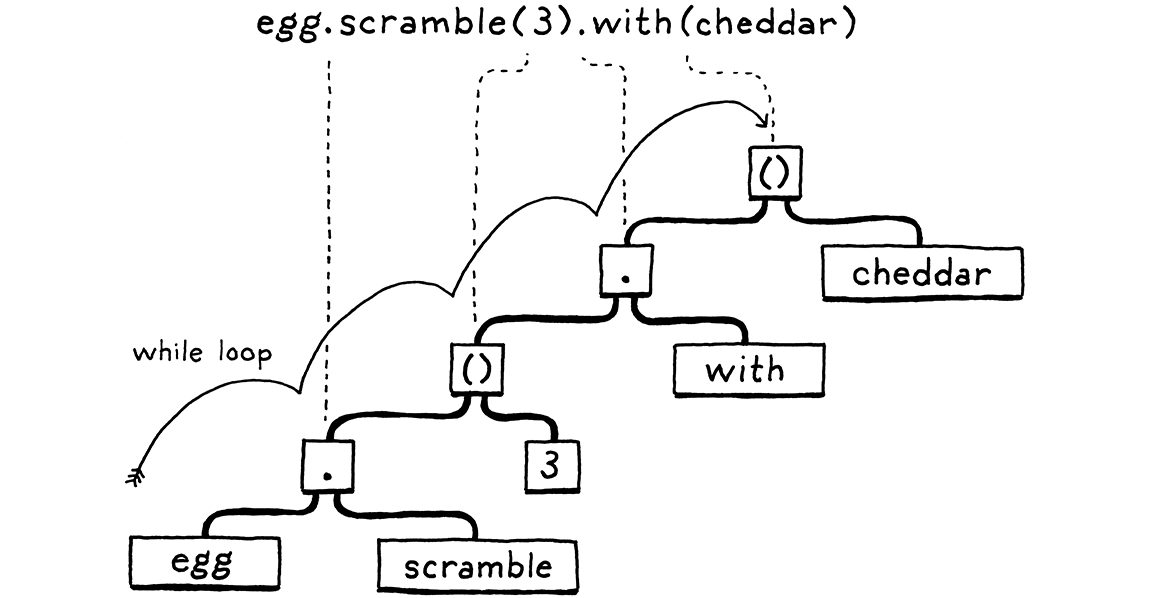
\includegraphics[width=\textwidth]{image/classes/zip.png}
\end{figure}

新的Expr.Get节点实例会被送入分析器。

\begin{code}{java}{}{lox/Resolver.java,在visitCallExpr()方法后添加}
  @Override
  public Void visitGetExpr(Expr.Get expr) {
    resolve(expr.object);
    return null;
  }
\end{code}

好吧,没什么好说的。因为属性是动态查找的,所以不会解析它们。在解析过程中,我们只递归到点符左边的表达式中。实际的属性访问发生在解释器中。

\begin{code}{java}{}{lox/Interpreter.java,在visitCallExpr()方法后添加}
  @Override
  public Object visitGetExpr(Expr.Get expr) {
    Object object = evaluate(expr.object);
    if (object instanceof LoxInstance) {
      return ((LoxInstance) object).get(expr.name);
    }

    throw new RuntimeError(expr.name,
        "Only instances have properties.");
  }
\end{code}

首先,我们对属性被访问的表达式求值。在Lox中,只有类的实例才具有属性。如果对象是其它类型(如数字),则对其执行getter是运行时错误。

如果该对象是LoxInstance,我们就要求它去查找该属性。现在必须给LoxInstance一些实际的状态了。一个map就行了。

\begin{code}{java}{2}{lox/LoxInstance.java,在LoxInstance类中添加}
  private LoxClass klass;
  private final Map<String, Object> fields = new HashMap<>();
  LoxInstance(LoxClass klass) {
\end{code}

map中的每个键是一个属性名称,对应的值就是该属性的值。查找实例中的一个属性:

\begin{code}{java}{}{lox/LoxInstance.java,在LoxInstance()方法后添加}
  Object get(Token name) {
    if (fields.containsKey(name.lexeme)) {
      return fields.get(name.lexeme);
    }

    throw new RuntimeError(name, 
        "Undefined property '" + name.lexeme + "'.");
  }
\end{code}

我们需要处理的一个有趣的边缘情况是,如果这个实例中\textit{不包含}给定名称的属性,会发生什么。我们可以悄悄返回一些假值,如nil,但是根据我对JavaScript等语言的经验,这种行为只是掩盖了错误,而没有做任何有用的事。相反,我们将它作为一个运行时错误。

因此,我们首先要做的就是看看这个实例中是否真的包含给定名称的字段。只有这样,我们才会返回其值。其它情况下,我们会引发一个错误。

注意我是如何从讨论“属性”转换到讨论“字段”的。这两者之间有一个微妙的区别。字段是直接保存在实例中的命名状态。属性是get表达式可能返回的已命名的\textit{东西}。每个字段都是一个属性,但是正如我们稍后将看到的,并非每个属性都是一个字段。

理论上,我们现在可以读取对象的属性。但是由于没有办法将任何状态真正填充到实例中,所以也没有字段可以访问。在我们测试读取之前,我们需要先支持写入。

\subsection{Set表达式}

setter和getter使用相同的语法,区别只是它们出现在赋值表达式的左侧。

\begin{code}{java}{}{}
someObject.someProperty = value;
\end{code}

在语言方面,我们扩展了赋值规则,允许在左侧使用点标识符。

\begin{ebnf}
assignment &\rightarrow\quad ( \quad call \quad \mathtt{"}.\mathtt{"} \quad )? \quad IDENTIFIER \quad \mathtt{"}=\mathtt{"} \quad assignment \\
&\;\;\vert\quad logic\_or \quad ;
\end{ebnf}

与getter不同,setter不使用链。但是,对call规则的引用允许在最后的点符号之前出现任何高优先级的表达式,包括任何数量的\textit{getters},如:

\begin{figure}[htbp]
  \centering
  
\includegraphics[width=\textwidth]{image/classes/setter.png}
\end{figure}

注意,这里只有最后一部分.meat是\textit{setter}。.omelette和.filling部分都是\textit{get}表达式。

就像我们有两个独立的AST节点用于变量访问和变量赋值一样,我们也需要一个setter节点来补充getter节点。

\begin{code}{java}{2}{tool/GenerateAst.java,在main()方法中添加}
      "Logical  : Expr left, Token operator, Expr right",
      "Set      : Expr object, Token name, Expr value",
      "Unary    : Token operator, Expr right",
\end{code}

也许你不记得了,我们在解析器中处理赋值的方法有点奇怪。在遇到=之前,我们无法轻易判断一系列标记是否一个赋值表达式的左侧部分。现在我们的赋值语法规则在左侧添加了call,它可以扩展为任意大的表达式,最后的=可能与我们需要知道是否正在解析赋值表达式的地方隔着很多标记。

相对地,我们的技巧就是把左边的表达式作为一个正常表达式来解析。然后,当我们在后面发现等号时,我们就把已经解析的表达式转换为正确的赋值语法树节点。

我们在该转换中添加另一个子句,将左边的Expr.Get表达式转化为相应的Expr.Set表达式。

\begin{code}{java}{2-4}{lox/Parser.java,在assignment()方法中添加}
        return new Expr.Assign(name, value);
      } else if (expr instanceof Expr.Get) {
        Expr.Get get = (Expr.Get)expr;
        return new Expr.Set(get.object, get.name, value);
      }
\end{code}

这就是语法解析。我们将该节点推入分析器中。

\begin{code}{java}{}{lox/Resolver.java,在visitLogicalExpr()方法后添加}
  @Override
  public Void visitSetExpr(Expr.Set expr) {
    resolve(expr.value);
    resolve(expr.object);
    return null;
  }
\end{code}

同样,像Expr.Get一样,属性本身是动态计算的,所以没有什么需要分析的。我们只需要递归到Expr.Set的两个子表达式中,即被设置属性的对象和它被设置的值。

这又会把我们引向解释器。

\begin{code}{java}{}{lox/Interpreter.java,在visitLogicalExpr()方法后添加}
  @Override
  public Object visitSetExpr(Expr.Set expr) {
    Object object = evaluate(expr.object);

    if (!(object instanceof LoxInstance)) { 
      throw new RuntimeError(expr.name,
                             "Only instances have fields.");
    }

    Object value = evaluate(expr.value);
    ((LoxInstance)object).set(expr.name, value);
    return value;
  }
\end{code}

我们先计算出被设置属性的对象,然后检查它是否是一个LoxInstance。如果不是,这就是一个运行时错误。否则,我们计算设置的值,并将其保存到该实例中。这一步依赖于LoxInstance中的一个新方法。

\begin{code}{java}{}{lox/LoxInstance.java,在get()方法后添加}
  void set(Token name, Object value) {
    fields.put(name.lexeme, value);
  }
\end{code}

这里没什么复杂的。我们把这些值之间塞入字段所在的Java map中。由于Lox允许在实例上自由创建新字段,所以不需要检查键是否已经存在。

\section{类中的方法}

你可以创建类的实例并将数据填入其中,但是类本身实际上并不能做任何事。实例只是一个map,而且所有的实例都是大同小异的。为了让它们更像是\textit{类}的实例,我们需要行为——方法。

我们的解析器已经解析了方法声明,所以我们在这部分做的不错。我们也不需要为方法\textit{调用}添加任何新的解析器支持。我们已经有了.(getter)和()(函数调用)。“方法调用”只是简单地将这些串在一起。

\begin{figure}[htbp]
  \centering
  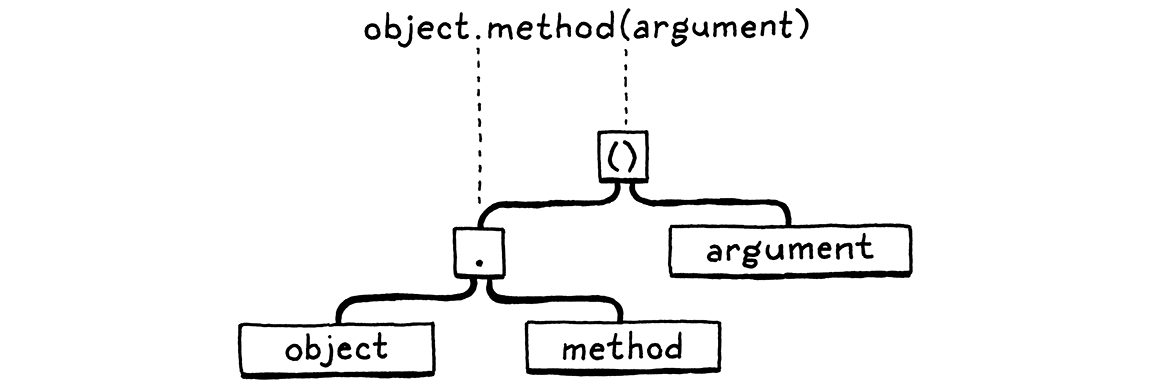
\includegraphics[width=\textwidth]{image/classes/method.png}
\end{figure}

这引出了一个有趣的问题。当这两个表达式分开时会发生什么?假设这个例子中的方法method是object的类中的一个方法,而不是实例中的一个字段,下面的代码应该做什么?

\begin{code}{java}{}{}
var m = object.method;
m(argument);
\end{code}

这个程序会“查找”该方法,并将结果(不管是什么)存储到一个变量中,稍后会调用该对象。允许这样吗?你能将方法作为实例中的一个函数来对待吗?

另一个方向呢?

\begin{code}{js}{}{}
class Box {}

fun notMethod(argument) {
  print "called function with " + argument;
}

var box = Box();
box.function = notMethod;
box.function("argument");
\end{code}

这个程序创建了一个实例,然后在它的一个字段中存储了一个函数。然后使用与方法调用相同的语法来调用该函数。这样做有用吗?

不同的语言对这些问题有不同的答案。人们可以就此写一篇论文。对于Lox来说,这两个问题的答案都是肯定的,它确实有效。我们有几个理由来证明这一点。对于第二个例子——调用存储在字段中的函数——我们想要支持它,是因为头等函数是有用的,而且将它们存储在字段中是一件很正常的事情。

第一个例子就比较晦涩了。一个场景是,用户通常希望能够在不改变程序含义的情况下,将子表达式赋值到一个局部变量中。你可以这样做:

\begin{code}{js}{}{}
breakfast(omelette.filledWith(cheese), sausage);
\end{code}

并将其变成这样:

\begin{code}{js}{}{}
var eggs = omelette.filledWith(cheese);
breakfast(eggs, sausage);
\end{code}

它做的是同样的事情。同样,由于方法调用中的.和()是两个独立的表达式,你似乎应该把查询部分提取到一个变量中,然后再调用它。我们需要仔细思考,当你查找一个方法时你得到的东西是什么,它如何作用,甚至是在一些奇怪的情况下,比如:

\begin{code}{js}{}{}
class Person {
  sayName() {
    print this.name;
  }
}

var jane = Person();
jane.name = "Jane";

var method = jane.sayName;
method(); // ?
\end{code}

如果你在某个实例上获取了一个方法的句柄,并在稍后再调用它,它是否能“记住”它是从哪个实例中提取出来的?方法内部的this是否仍然指向原始的那个对象?

下面有一个更变态的例子,可以摧毁你的大脑:

\begin{code}{js}{}{}
class Person {
  sayName() {
    print this.name;
  }
}

var jane = Person();
jane.name = "Jane";

var bill = Person();
bill.name = "Bill";

bill.sayName = jane.sayName;
bill.sayName(); // ?
\end{code}

最后一行会因为\textit{调用}方法的实体是bill而打印“Bill”,还是因为我们第一次获取方法的实例是jane而打印“Jane”。

在Lua和JavaScript中,同样的代码会打印"Bill"。这些语言并没有真正的“方法”的概念。所有东西都类似于字段中的函数,所以并不清楚jane是否更应该比bill“拥有”sayName。

不过,Lox有真正的类语法,所以我们确实知道哪些可调用的东西是方法,哪些是函数。因此,像Python、C\#和其他语言一样,当方法第一次被获取时,我们会让方法与原始实例this进行"绑定"。Python将这些绑定的方法称为\textbf{bound methods}(绑定方法)。

在实践中,这通常也是你想要的。如果你获取到了某个对象中一个方法的引用,这样你以后就可以把它作为一个回调函数使用,你想要记住它所属的实例,即使这个回调被存储在其它对象的字段中。

好吧,这里有很多语义需要装到你的脑子里。暂时先不考虑那些边缘情况了,我们以后再讲。现在,让我们先把基本的方法调用做好。我们已经解析了类主体内的方法声明,所以下一步就是对其分析。

\begin{code}{java}{2-5}{lox/Resolver.java,在visitClassStmt()方法内添加}
    define(stmt.name);
    for (Stmt.Function method : stmt.methods) {
      FunctionType declaration = FunctionType.METHOD;
      resolveFunction(method, declaration); 
    }
    return null;
\end{code}

我们遍历类主体中的方法,并调用我们已经写好的用来处理函数声明的resolveFunction()方法。唯一的区别在于,我们传入了一个新的FunctionType枚举值。

\begin{code}{java}{3}{lox/Resolver.java,在FunctionType枚举中添加代码,在上1行末尾添加“,”}
    NONE,
    FUNCTION,
    METHOD
  }
\end{code}

这一点在我们分析this表达式时很重要。现在还不用担心这个问题。有趣的部分在解释器中。

\begin{code}{java}{2-8}{lox/Interpreter.java,在visitClassStmt()方法中替换1行}
    environment.define(stmt.name.lexeme, null);
    Map<String, LoxFunction> methods = new HashMap<>();
    for (Stmt.Function method : stmt.methods) {
      LoxFunction function = new LoxFunction(method, environment);
      methods.put(method.name.lexeme, function);
    }

    LoxClass klass = new LoxClass(stmt.name.lexeme, methods);
    environment.assign(stmt.name, klass);
\end{code}

当我们解释一个类声明语句时,我们把类的语法表示(其AST节点)变成它的运行时表示。现在,我们也需要对类中包含的方法进行这样的操作。每个方法声明都会变成一个LoxFunction对象。

我们把所有这些都打包到一个map中,以方法名称作为键。这些数据存储在LoxClass中。

\begin{code}{java}{2-7}{lox/LoxClass.java,在类LoxClass中,替换4行}
  final String name;
  private final Map<String, LoxFunction> methods;

  LoxClass(String name, Map<String, LoxFunction> methods) {
    this.name = name;
    this.methods = methods;
  }
  @Override
  public String toString() {
\end{code}

实例存储状态,类存储行为。LoxInstance包含字段的map,而LoxClass包含方法的map。虽然方法是归类所有,但仍然是通过类的实例来访问。

\begin{code}{java}{5-6}{lox/LoxInstance.java,在get()方法中添加}
  Object get(Token name) {
    if (fields.containsKey(name.lexeme)) {
      return fields.get(name.lexeme);
    }
    LoxFunction method = klass.findMethod(name.lexeme);
    if (method != null) return method;
    throw new RuntimeError(name, 
        "Undefined property '" + name.lexeme + "'.");
\end{code}

在实例上查找属性时,如果我们没有找到匹配的字段,我们就在实例的类中查找是否包含该名称的方法。如果找到,我们就返回该方法。这就是“字段”和“属性”之间的区别变得有意义的地方。当访问一个属性时,你可能会得到一个字段(存储在实例上的状态值),或者你会得到一个实例类中定义的方法。

方法是通过下面的代码进行查找的:

\begin{code}{java}{}{lox/LoxClass.java,在LoxClass()方法后添加}
  LoxFunction findMethod(String name) {
    if (methods.containsKey(name)) {
      return methods.get(name);
    }

    return null;
  }
\end{code}

你大概能猜到这个方法后面会变得更有趣。但是现在,在类的方法表中进行简单的映射查询就足够了。试一下:

\begin{code}{js}{}{}
class Bacon {
  eat() {
    print "Crunch crunch crunch!";
  }
}

Bacon().eat(); // Prints "Crunch crunch crunch!".
\end{code}

\section{This}

我们可以在对象上定义行为和状态,但是它们并没有被绑定在一起。在一个方法中,我们没有办法访问“当前”对象(调用该方法的实例)的字段,也不能调用同一个对象的其它方法。

为了获得这个实例,它需要一个名称。Smalltalk、Ruby和Swift使用“self”。Simula、C++、Java等使用“this”。Python按惯例使用“self”,但从技术上讲,你可以随便叫它什么。

对于Lox来说,因为我们通常遵循Java风格,我们会使用“this”。在方法体中,this表达式计算结果为调用该方法的实例。或者,更确切地说,由于方法是分为两个步骤进行访问和调用的,因此它会引用调用方法的对象。

这使得我们的工作更加困难。请看:

\begin{code}{js}{}{}
class Egotist {
  speak() {
    print this;
  }
}

var method = Egotist().speak;
method();
\end{code}

在倒数第二行,我们从该类的一个实例中获取到了指向speak()的引用。这个操作会返回一个函数,并且该函数需要记住它来自哪个实例,这样稍后在最后一行,当函数被调用时,它仍然可用找到对应实例。

我们需要在方法被访问时获取到this,并将其附到函数上,这样当我们需要的时候它就一直存在。嗯...一种存储函数周围的额外数据的方法,嗯?听起来很像一个闭包,不是吗?

如果我们把this定义为在查找方法时返回的函数外围环境中的一个隐藏变量,那么稍后在方法主体中使用this时就可以找到它了。LoxFunction已经具备了保持外围环境的能力,所以我们已经有了需要的机制。

我们通过一个例子来看看它是如何工作的:

\begin{code}{js}{}{}
class Cake {
  taste() {
    var adjective = "delicious";
    print "The " + this.flavor + " cake is " + adjective + "!";
  }
}

var cake = Cake();
cake.flavor = "German chocolate";
cake.taste(); // Prints "The German chocolate cake is delicious!".
\end{code}

当我们第一次执行类定义时,我们为taste()创建了一个LoxFunction。它的闭包是类外围的环境,在这个例子中就是全局环境。所以我们在类的方法map中保存的LoxFunction看起来像是这样的:

\begin{figure}[htbp]
  \centering
  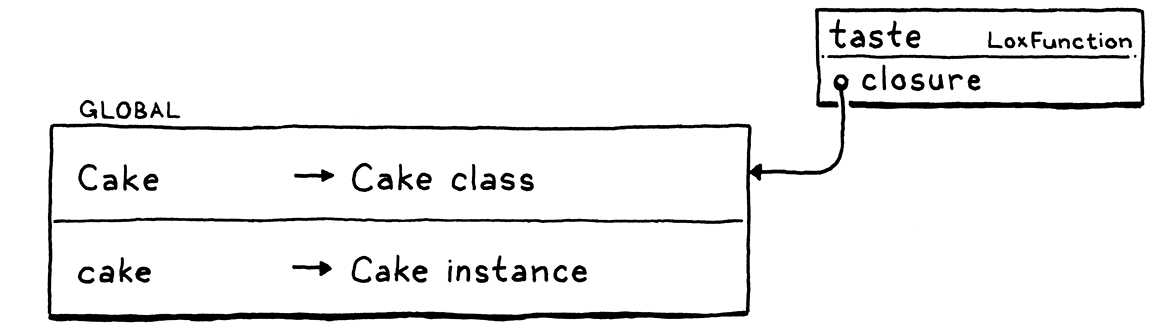
\includegraphics[width=\textwidth]{image/classes/closure.png}
\end{figure}

当我们执行cake.taste这个get表达式时,我们会创建一个新的环境,其中将this绑定到了访问该方法的对象(这里是cake)。然后我们创建一个\textit{新}的LoxFunction,它的代码与原始的代码相同,但是使用新环境作为其闭包。

\begin{figure}[htbp]
  \centering
  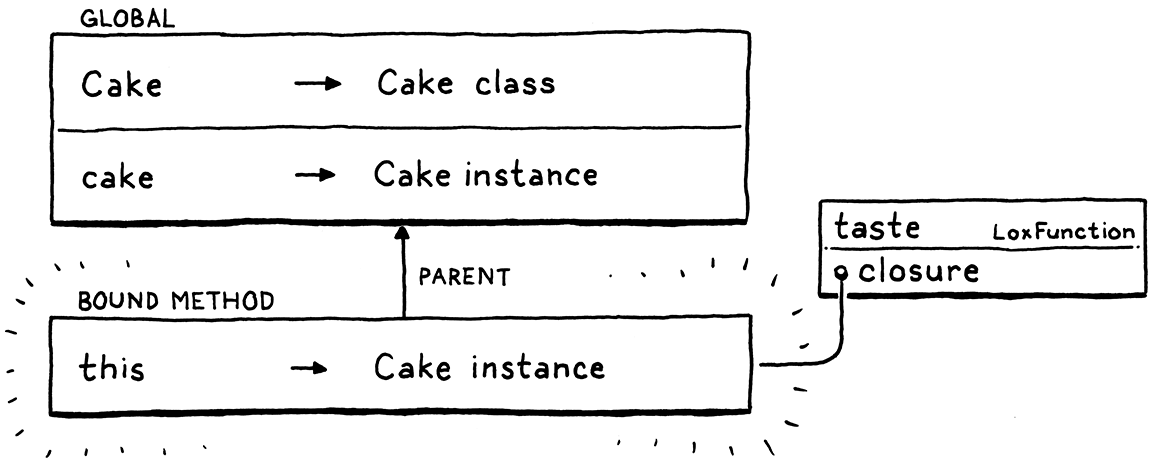
\includegraphics[width=\textwidth]{image/classes/bound-method.png}
\end{figure}

这个是在执行方法名的get表达式时返回的LoxFunction。当这个函数稍后被一个()表达式调用时,我们像往常一样为方法主体创建一个环境。

\begin{figure}[htbp]
  \centering
  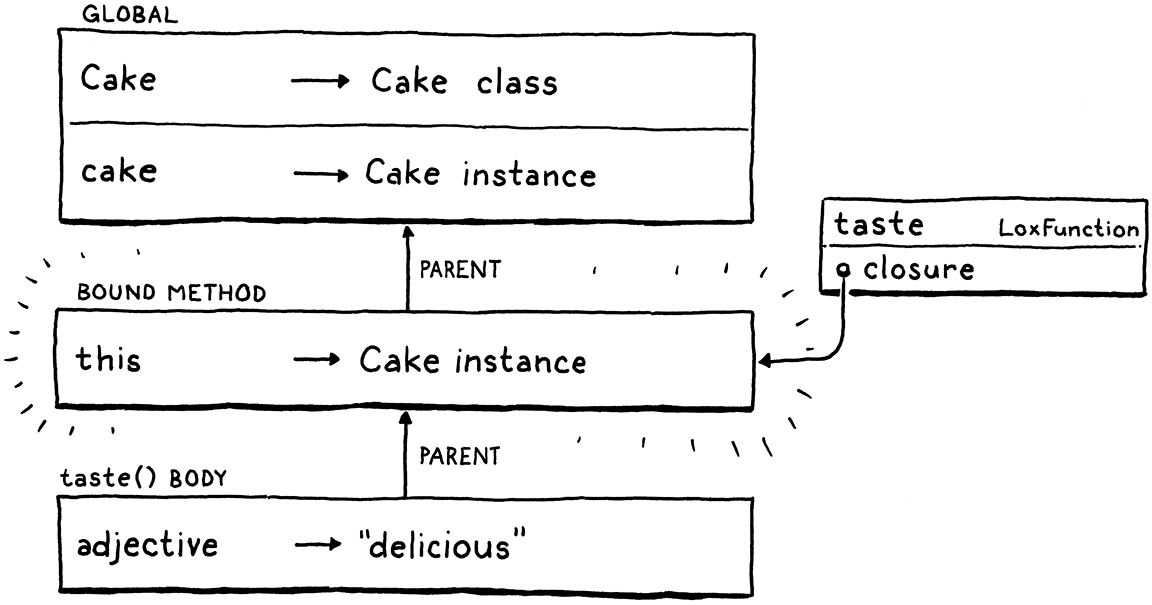
\includegraphics[width=\textwidth]{image/classes/call.png}
\end{figure}

主体环境的父环境,也就是我们先前创建并在其中将this绑定到当前对象的那个环境。因此,在函数主体内使用this都可以成功解析到那个实例。

重用环境代码来实现this时,也需要注意方法和函数交互的情况,比如:

\begin{code}{js}{}{}
class Thing {
  getCallback() {
    fun localFunction() {
      print this;
    }

    return localFunction;
  }
}

var callback = Thing().getCallback();
callback();
\end{code}

例如,在JavaScript中,在一个方法中返回一个回调函数是很常见的。这个回调函数可能希望保留对方法所关联的原对象(this值)的访问。我们现有的对闭包和环境链的支持应该可以正确地做到这一点。

让我们把它写出来。第一步是为this添加新的语法。

\begin{code}{java}{2}{tool/GenerateAst.java,在main()方法中添加}
      "Set      : Expr object, Token name, Expr value",
      "This     : Token keyword",
      "Unary    : Token operator, Expr right",
\end{code}

解析很简单,因为它是已经被词法解析器当作关键字识别出来的单个词法标记。

\begin{code}{java}{3}{lox/Parser.java,在primary()方法中添加}
      return new Expr.Literal(previous().literal);
    }
    if (match(THIS)) return new Expr.This(previous());
    if (match(IDENTIFIER)) {
\end{code}

当进入分析器后,就可以看到this是如何像变了一样作用的。

\begin{code}{java}{}{lox/Resolver.java,在visitSetExpr()方法后添加}
  @Override
  public Void visitThisExpr(Expr.This expr) {
    resolveLocal(expr, expr.keyword);
    return null;
  }
\end{code}

我们使用this作为“变量”的名称,并像其它局部变量一样对其分析。当然,现在这是行不通的,因为“this”没有在任何作用域进行声明。我们在visitClassStmt()方法中解决这个问题。

\begin{code}{java}{2-3}{lox/Resolver.java,在visitClassStmt()方法中添加}
    define(stmt.name);
    beginScope();
    scopes.peek().put("this", true);
    for (Stmt.Function method : stmt.methods) {
\end{code}

在我们开始分析方法体之前,我们推入一个新的作用域,并在其中像定义变量一样定义“this”。然后,当我们完成后,会丢弃这个外围作用域。

\begin{code}{java}{2}{lox/Resolver.java,在visitClassStmt()方法中添加}
    }
    endScope();
    return null;
\end{code}

现在,只要遇到this表达式(至少是在方法内部),它就会解析为一个“局部变量”,该变量定义在方法体块之外的隐含作用域中。

分析器对this有一个新的\textit{作用域},所以解释器需要为它创建一个对应的\textit{环境}。记住,我们必须始终保持分析器的作用域链与解释器的链式环境保持同步。在运行时,我们在找到实例上的方法后创建环境。我们把之前那行直接返回方法对应LoxFunction的代码替换如下:

\begin{code}{java}{2}{lox/LoxInstance.java,在get()方法中替换1行}
    LoxFunction method = klass.findMethod(name.lexeme);
    if (method != null) return method.bind(this);
    throw new RuntimeError(name, 
        "Undefined property '" + name.lexeme + "'.");
\end{code}

注意这里对bind()的新调用。该方法看起来是这样的:

\begin{code}{java}{}{lox/LoxFunction.java,在LoxFunction()方法后添加}
  LoxFunction bind(LoxInstance instance) {
    Environment environment = new Environment(closure);
    environment.define("this", instance);
    return new LoxFunction(declaration, environment);
  }
\end{code}

这没什么好说的。我们基于方法的原始闭包创建了一个新的环境。就像是闭包内的闭包。当方法被调用时,它将变成方法体对应环境的父环境。

我们将this声明为该环境中的一个变量,并将其绑定到给定的实例(即方法被访问时的实例)上。就是这样,现在返回的LoxFunction带着它自己的小持久化世界,其中的“this”被绑定到对象上。

剩下的任务就是解释那些this表达式。与分析器类似,与解释变量表达式是一样的。

\begin{code}{java}{}{lox/Interpreter.java,在visitSetExpr()方法后添加}
  @Override
  public Object visitThisExpr(Expr.This expr) {
    return lookUpVariable(expr.keyword, expr);
  }
\end{code}

来吧,用前面那个蛋糕的例子试一试。通过添加不到20行代码,我们的解释器就能处理方法内部的this,甚至能以各种奇怪的方式与嵌套类、方法内部的函数、方法句柄等进行交互。

\subsection{this的无效使用}

等一下,如果你尝试在方法之外使用this会怎么样?比如:

\begin{code}{java}{}{}
print this;
\end{code}

或者:

\begin{code}{js}{}{}
fun notAMethod() {
  print this;
}
\end{code}

如果你不在一个方法中,就没有可供this指向的实例。我们可以给它一些默认值如nil或者抛出一个运行时错误,但是用户显然犯了一个错误。他们越早发现并纠正这个错误,就会越高兴。

我们的分析过程是一个静态检测这个错误的好地方。它已经检测了函数之外的return语句。我们可以针对this做一些类似的事情。在我们现有的FunctionType枚举的基础上,我们定义一个新的ClassType枚举。

\begin{code}{java}{2-7}{lox/Resolver.java,在FunctionType枚举后添加}
  }
  private enum ClassType {
    NONE,
    CLASS
  }

  private ClassType currentClass = ClassType.NONE;
  void resolve(List<Stmt> statements) {
\end{code}

是的,它可以是一个布尔值。当我们谈到继承时,它会扩展第三个值,因此使用了枚举。我们还添加了一个相应的字段currentClass。它的值告诉我们,在遍历语法树时,我们目前是否在一个类声明中。它一开始是NONE,意味着我们不在类中。

当我们开始分析一个类声明时,我们会改变它。

\begin{code}{java}{2-3}{lox/Resolver.java,在visitClassStmt()方法中添加}
  public Void visitClassStmt(Stmt.Class stmt) {
    ClassType enclosingClass = currentClass;
    currentClass = ClassType.CLASS;
    declare(stmt.name);
\end{code}

与currentFunction一样,我们将字段的前一个值存储在一个局部变量中。这样我们可以在JVM中保持一个currentClass的栈。如果一个类嵌套在另一个类中,我们就不会丢失对前一个值的跟踪。

一旦这么方法完成了分析,我们通过恢复旧值来“弹出”堆栈。

\begin{code}{java}{2}{lox/Resolver.java,在visitClassStmt()方法中添加}
    endScope();
    currentClass = enclosingClass;
    return null;
\end{code}

当我们解析this表达式时,如果表达式没有出现在一个方法体内,currentClass就为我们提供了报告错误所需的数据。

\begin{code}{java}{2-6}{lox/Resolver.java,在visitThisExpr()方法中添加}
  public Void visitThisExpr(Expr.This expr) {
    if (currentClass == ClassType.NONE) {
      Lox.error(expr.keyword,
          "Can't use 'this' outside of a class.");
      return null;
    }
    resolveLocal(expr, expr.keyword);
\end{code}

这应该能帮助用户正确地使用this,并且它使我们不必在解释器运行时中处理这个误用问题。

\section{构造函数和初始化}

我们现在几乎可以用类来做任何事情,而当我们接近本章结尾时,却发现自己奇怪地专注于开头。方法和字段让我们把状态和行为封装在一起,这样一个对象就能始终保持在有效的配置状态。但我们如何确保一个全新的对象是以良好的状态开始的?

为此,我们需要构造函数。我发现它们是语言设计中最棘手的部分之一,如果你仔细观察大多数其它语言,就会发现围绕着对象构造的缺陷,设计的接缝并不完全吻合。也许在一开始就存在本质上的混乱。

“构造”一个对象实际上是一对操作:

\begin{enumerate}
  \item 运行时为一个新的实例*分配*所需的内存。在多数语言中,这个操作是在用户代码可以访问的层面之下的基础层完成的。
  \item 然后,用户提供的一大块代码被调用,以初始化未成形的对象。
\end{enumerate}

当我们听到“构造函数”时,我们往往会想到后者,但语言本身在此之前通常已经为我们做了一些基础工作。事实上,我们的Lox解释器在创建一个新的LoxInstance对象时已经涵盖了这一点。

我们现在要做的是剩下的部分——用户自定义的初始化。对于为类建立新对象的这块代码,不同的语言有不同的说法。C++、Java和C\#使用一个名字与类名相匹配的方法。Ruby 和 Python 称之为 init()。后者又好又简短,所以我们采用它。

在LoxClass的LoxCallable实现中,我们再增加几行。

\begin{code}{java}{3-6}{lox/LoxClass.java,在call()方法中添加}
                     List<Object> arguments) {
    LoxInstance instance = new LoxInstance(this);
    LoxFunction initializer = findMethod("init");
    if (initializer != null) {
      initializer.bind(instance).call(interpreter, arguments);
    }
    return instance;
\end{code}

当一个类被调用时,在LoxInstance被创建后,我们会寻找一个"init"方法。如果我们找到了,我们就会立即绑定并调用它,就像普通的方法调用一样。参数列表直接透传。

这个参数列表意味着我们也需要调整类声明其元数的方式。

\begin{code}{java}{}{}
  public int arity() {
\end{code}

\begin{code}{java}{2-4}{lox/LoxClass.java,在arity()方法中替换1行:}
  public int arity() {
    LoxFunction initializer = findMethod("init");
    if (initializer == null) return 0;
    return initializer.arity();
  }
\end{code}

如果有初始化方法,该方法的元数就决定了在调用类本身的时候需要传入多少个参数。但是,为了方便起见,我们并不要求类定义初始化方法。如果你没有初始化方法,元数仍然是0。

基本上就是这样了。因为我们在调用init()方法之前已经将其绑定,所以它可以在方法体内访问this。这样,连同传递给类的参数,你就可以按照自己的意愿设置新实例了。

\subsection{直接执行init()}

像往常一样,探索这一新的语义领域会催生出一些奇怪的事物。考虑一下:

\begin{code}{js}{}{}
class Foo {
  init() {
    print this;
  }
}

var foo = Foo();
print foo.init();
\end{code}

你能否通过直接调用对象的init()方法对其进行“重新初始化”?如果可以,它的返回值是什么?一个合理的答案应该是nil,因为这是方法主体返回的内容。

然而,我通常不喜欢为满足实现而妥协,如果我们让init()方法总是返回this(即使是被直接调用时),它会使clox中的构造函数实现更加简单。为了保持jlox与之兼容,我们在LoxFunction中添加了一些针对特殊情况的代码。

\begin{code}{java}{3}{lox/LoxFunction.java,在call()方法中添加}
      return returnValue.value;
    }
    if (isInitializer) return closure.getAt(0, "this");
    return null;
\end{code}

如果该函数是一个初始化方法,我们会覆盖实际的返回值并强行返回this。这个操作依赖于一个新的isInitializer字段。

\begin{code}{java}{2-5}{lox/LoxFunction.java,在LoxFunction类中,替换1行:}
  private final Environment closure;
  private final boolean isInitializer;

  LoxFunction(Stmt.Function declaration, Environment closure, boolean isInitializer) {
    this.isInitializer = isInitializer;
    this.closure = closure;
    this.declaration = declaration;
\end{code}

我们不能简单地检查LoxFunction的名字是否为“init”,因为用户已经定义了一个同名的\textit{函数}。在这种情况下,是没有this可供返回的。为了避免这种奇怪的边缘情况,我们将直接存储LoxFunction是否表示一个初始化方法。这意味着我们需要回头修正我们创建LoxFunctions的几个地方。

\begin{code}{java}{2}{lox/Interpreter.java,在visitFunctionStmt()方法中,替换1行:}
  public Void visitFunctionStmt(Stmt.Function stmt) {
    LoxFunction function = new LoxFunction(stmt, environment, false);
    environment.define(stmt.name.lexeme, function);
\end{code}

对于实际的函数声明,isInitializer取值总是false。对于方法来说,我们检查其名称。

\begin{code}{java}{2-3}{lox/Interpreter.java,在visitClassStmt()方法中,替换1行:}
    for (Stmt.Function method : stmt.methods) {
      LoxFunction function = new LoxFunction(method, environment,
          method.name.lexeme.equals("init"));
      methods.put(method.name.lexeme, function);
\end{code}

然后在bind()方法,在创建闭包并将this绑定到新方法时,我们将原始方法的值传递给新方法。

\begin{code}{java}{2-3}{lox/LoxFunction.java,在bind()方法中,替换1行:}
    environment.define("this", instance);
    return new LoxFunction(declaration, environment,
                           isInitializer);
  }
\end{code}

\subsection{从init()返回}

我们还没有走出困境。我们一直假设用户编写的初始化方法不会显式地返回一个值,因为大多数构造函数都不会。如果用户尝试这样做会发生什么:

\begin{code}{java}{}{}
class Foo {
  init() {
    return "something else";
  }
}
\end{code}

这肯定不会按照用户的期望执行,所以我们不妨把它作为一种静态错误。回到分析器中,我们为FunctionType添加另一种情况。

\begin{code}{java}{2}{lox/Resolver.java,在FunctionType枚举中添加}
    FUNCTION,
    INITIALIZER,
    METHOD
\end{code}

我们通过被访问方法的名称来确定我们是否在分析一个初始化方法。

\begin{code}{java}{2-4}{lox/Resolver.java,在visitClassStmt()方法中添加}
      FunctionType declaration = FunctionType.METHOD;
      if (method.name.lexeme.equals("init")) {
        declaration = FunctionType.INITIALIZER;
      }
      resolveFunction(method, declaration); 
\end{code}

当我们稍后遍历return语句时,我们会检查该字段,如果从init()方法内部返回一个值时就抛出一个错误。

\begin{code}{java}{2-5}{lox/Resolver.java,在visitReturnStmt()方法中添加}
    if (stmt.value != null) {
      if (currentFunction == FunctionType.INITIALIZER) {
        Lox.error(stmt.keyword,
            "Can't return a value from an initializer.");
      }
      resolve(stmt.value);
\end{code}

我们\textit{仍然}没有结束。我们静态地禁止了从初始化格式返回一个值,但是你仍然可用使用一个空的return。

\begin{code}{java}{}{}
class Foo {
  init() {
    return;
  }
}
\end{code}

有时候这实际上是有用的,所以我们不想完全禁止它。相对地,它应该返回this而不是nil。这在LoxFunction中很容易解决。

\begin{code}{java}{2}{lox/LoxFunction.java,在call()方法中添加}
    } catch (Return returnValue) {
      if (isInitializer) return closure.getAt(0, "this");
      return returnValue.value;
\end{code}

如果我们在一个初始化方法中执行return语句时,我们仍然返回this,而不是返回值(该值始终是nil)。

吁!这是一大堆任务,但是我们的收获是,我们的小解释器已经成长为一个完整的编程范式。类、方法、字段、this以及构造函数,我们的语言看起来已经非常成熟了。

\section{挑战}

\begin{enumerate}
  \item 我们有实例上的方法,但是没有办法定义可以直接在类对象上调用的“静态”方法。添加对它们的支持,在方法之前使用class关键字指示该方法是一个挂载在类对象上的静态方法。

   \begin{code}{java}{}{}
   class Math {
     class square(n) {
       return n * n;
     }
   }
   
   print Math.square(3); // Prints "9".
   \end{code}

  你可以用你喜欢的方式解决这问题,但是Smalltalk和Ruby使用的“metaclasses”是一种特别优雅的方法。\textit{提示:让LoxClass继承LoxInstance,然后开始实现。}

  \item 大多数现代语言都支持“getters”和“setters”——类中的成员,看起来像是字段的读写,但实际上执行的用户自定义的代码。扩展Lox以支持getter方法。这些方法在声明时没有参数列表。当访问具有该名称的属性时,会执行getter的主体。

   \begin{code}{java}{}{}
   class Circle {
     init(radius) {
       this.radius = radius;
     }
   
     area {
       return 3.141592653 * this.radius * this.radius;
     }
   }
   
   var circle = Circle(4);
   print circle.area; // Prints roughly "50.2655".
   \end{code}

  \item Python和JavaScript允许你从对象自身的方法之外的地方自由访问对象的字段。Ruby和Smalltalk封装了实例状态。只有类上的方法可以访问原始字段,并且由类来决定哪些状态被暴露。大多数静态类型的语言都提供了像private和public这样的修饰符,以便按成员维度控制类的哪些部分可以被外部访问。

  这些方式之间的权衡是什么?为什么一门语言可能会更偏爱某一种方法?
\end{enumerate}

\section{设计笔记:原型与功率}

在本章中,我们引入了两个新的运行时实体,LoxClass和LoxInstance。前者是对象的行为所在,后者则是状态所在。如果你可以在LoxInstance的单个对象中定义方法,会怎么样?这种情况下,我们根本就不需要LoxClass。LoxInstance将是一个用于定义对象行为和状态的完整包。

我们仍然需要一些方法,在没有类的情况下,可以跨多个实例重用对象行为。我们可以让一个LoxInstance直接委托给另一个LoxInstance来重用它的字段和方法,有点像继承。

用户可以将他们的程序建模为一组对象,其中一些对象相互委托以反映共性。用作委托的对象代表“典型”或“原型”对象,会被其它对象完善。结果就是会有一个更简单的运行时,只有一个内部结构LoxInstance。

这就是这种范式的名称“原型”的由来。它是由David Ungar和Randall Smith在一种叫做Self的语言中发明的。他们从Smalltalk开始,按照上面的练习,看他们能把它缩减到什么程度,从而想到了这个方法。

长期以来,原型一直是学术上的探索,它是一个引人入胜的东西,也产生了有趣的研究,但是并没有在更大的编程世界中产生影响。直到Brendan Eich把原型塞进JavaScript,然后迅速风靡世界。关于JavaScript中的原型,人们已经写了很多(许多)文字。这是否能够表明原型是出色的还是令人困惑的,或者兼而有之?这是一个开放的问题。

我不会去讨论原型对于一门语言来说是不是一个好主意。基于原型和基于类的语言我都做过,我对两者的看法很复杂。我想讨论的是\textit{简单性}在一门语言中的作用。

原型比类更简单——语言实现者要编写的代码更少,语言用户要学习和理解的概念更少。这是否意味着它让语言变得更好呢?我们这些语言书呆子有一种迷恋极简主义的倾向。就我个人而言,我认为简单性只是一部分。我们真正想给用户的是功率,我将其定义为:

\begin{code}{js}{}{}
power = breadth * ease ÷ complexity
功率 = 广度 * 易用性 ÷ 复杂性
\end{code}

这些都不是精确的数字度量。我这里用数学作比喻,而不是实际的量化。

\begin{itemize}
  \item \textbf{广度}是语言可以表达的不同事物的范围。C语言具有很大的广度——从操作系统到用户应用程序再到游戏,它被广泛使用。像AppleScript和Matlab这样的特定领域语言的广度相对较小。
  \item 易用性是指用户付出多少努力就可以用语言做想做的事。“可用性Usability”是另一个概念,它包含的内容比我想要表达的更多。“高级”语言往往比“低级”语言更容易使用。大多数语言都有一个核心,对它们来说,有些东西比其它的更容易表达。
  \item 复杂性是指语言的规模(包括其运行时、核心库、工具、生态等)有多大。人们谈论一种语言的规范有多少页,或者它有多少个关键词。这是指用户在使用系统之前,必须在先学习多少东西,才能产生效益。它是简单性的反义词。
\end{itemize}

降低复杂性确实可以提高功率,分母越小,得到的值就越大,所以我们直觉认为“简单的是好的”是对的。然而,在降低复杂性时,我们必须注意不要在这个过程中牺牲广度或易用性,否则总功率可能会下降。如果去掉字符串,Java将变成一种严格意义上的简单语言,但它可能无法很好地处理文本操作任务,也不会那么容易完成事情。

因此,关键就在于找到可以省略的意外复杂性,也就是哪些没有通过增加语言广度或语言易用性来体现其重要性的语言特性与交互。

如果用户想用对象的类别来表达他们的程序,那么在语言中加入类就能提高这类操作的便利性,希望能有足够大的提升幅度来弥补所增加的复杂性。但如果这不是用户使用您的语言的方式,那么无论如何都不要使用类。

\chapter{继承}

\epigraph{我们曾经是海里一团一团的东西,然后是鱼,然后是蜥蜴、老鼠、猴子,以及介于其间的数百种形态。这只手曾经是鳍,这只手曾经是爪子!在我人类的嘴里,有狼的尖牙,有兔子的凿齿,还有牛的磨牙!我们的血和我们曾经生活的大海一样咸!当我们受到惊吓时,我们皮肤上的毛发会竖起来,就像我们有毛时一样。我们就是历史!我们在成为我们的路上曾拥有的一切,我们仍然拥有。}{特里}

你能相信吗?我们已经到了第二部分的最后一章。我们几乎已经完成了第一个Lox解释器。上一章中是一大堆错综复杂的面向对象特性。我无法将这些内容完全解开,但是我设法拆出来一块。在这一章,我们会添加继承来完成Lox中对类的支持。

继承出现在面向对象语言中,可以追溯到第一种语言Simula。早些时候,克里斯汀·尼加德(Kristen Nygaard)和奥勒-约翰·达尔(Ole-Johan Dahl)注意到,在他们编写的模拟程序中,不同类之间存在共性。继承为他们提供了一种重用相似部分代码的方法。

\section{超类和子类}

鉴于这个概念叫“继承”,你可能希望他们会选择一个一致的比喻,把类称为“父”类和“子”类,但这太简单了。早在很久以前,C. A. R. Hoare就创造了“subclass”这个术语,指的是完善另一种类型的记录类型。Simula借用了这个术语来指代一个继承自另一个类的类。我认为直到Smalltalk出现后,才有人将这个词的拉丁前缀取反义,用超类(superclass)指代这种关系的另一方。

我们在Lox中支持继承的第一步是找到声明类时指定超类的方法。这方面有很多不同的语法。C++和C\#在子类的名字后面加一个:,然后是超类的名字。Java使用extends而不是冒号。Python则把超类放在类名后面的小括号里。Simula把超类的名字放在关键字class之前。

游戏已经到了后期,我宁愿不在词法分析器中添加新的保留字或标记。我们没有extends或:,所以我们遵循Ruby来使用小于号(<)。

\begin{code}{java}{}{}
class Doughnut {
  // General doughnut stuff...
}

class BostonCream < Doughnut {
  // Boston Cream-specific stuff...
}
\end{code}

为了在语法中实现这一点,我们在目前的classDecl规则中加一个新的可选子句。

\begin{ebnf}
classDecl &\rightarrow\quad \mathtt{"}class\mathtt{"} \quad IDENTIFIER \quad ( \quad \mathtt{"}<\mathtt{"} \quad IDENTIFIER \quad )? \\
          &\quad\quad \mathtt{"}{\mathtt{"} \quad function* \quad \mathtt{"}}\mathtt{"} \quad ;
\end{ebnf}

在类的名称后面,可以有一个<,后跟超类的名称。超类子句是可选的,因为一个类不一定要有超类。与Java等面向对象的语言不同,Lox没有所有东西都继承的一个根“Object”类,所以当你省略超类子句时,该类就没有超类,甚至连隐含的都没有。

我们想在类声明的AST节点中捕捉这个新语法。

\begin{code}{java}{2}{tool/GenerateAst.java,在main()方法中,替换1行:}
      "Block      : List<Stmt> statements",
      "Class      : Token name, Expr.Variable superclass,List<Stmt.Function> methods",
      "Expression : Expr expression",
\end{code}

你可能会惊讶,我们把超类的名字存为一个Expr.Variable,而不是一个Token。语法将一个超类子句限制为一个标识符,但是在运行时,这个标识符是当作变量访问来执行的。在解析器早期将名称封装在Expr.Variable内部,这样可以给我们提供一个对象,在分析器中可以将分析信息附加在其中。

新的解析器代码直接遵循语法。

\begin{code}{java}{2-6}{lox/Parser.java,在classDeclaration()中添加}
    Token name = consume(IDENTIFIER, "Expect class name.");
    Expr.Variable superclass = null;
    if (match(LESS)) {
      consume(IDENTIFIER, "Expect superclass name.");
      superclass = new Expr.Variable(previous());
    }
    consume(LEFT_BRACE, "Expect '{' before class body.");
\end{code}

一旦我们(可能)解析到一个超类声明,就将其保存到AST节点中。

\begin{code}{java}{2}{lox/Parser.java,在classDeclaration()方法中,替换1行:}
    consume(RIGHT_BRACE, "Expect '}' after class body.");
    return new Stmt.Class(name, superclass, methods);
  }
\end{code}

如果我们没有解析到超类子句,超类表达式将是null。我们必须确保后面的操作会对其进行检查。首先是分析器。

\begin{code}{java}{2-4}{lox/Resolver.java,在visitClassStmt()方法中添加}
    define(stmt.name);
    if (stmt.superclass != null) {
      resolve(stmt.superclass);
    }
    beginScope();
\end{code}

类声明的AST节点有一个新的子表达式,所以我们要遍历并分析它。因为类通常是在顶层声明的,超类的名称很可能是一个全局变量,所以这一步通常没有什么作用。然而,Lox运行在区块内的类声明,所以超类名称有可能指向一个局部变量。在那种情况下,我们需要保证能被它被分析。

即使是善意的程序员有时也会写出奇怪的代码,所以在这里我们需要考虑一个愚蠢的边缘情况。看看这个:

\begin{code}{ruby}{}{}
class Oops < Oops {}
\end{code}

这种代码不可能做什么有用的事情,如果我们尝试让运行时去执行它,将会打破解释器对继承链中没有循环的期望。最安全的做法是静态地检测这种情况,并将其作为一个错误报告出来。

\begin{code}{java}{2-6}{lox/Resolver.java,在visitClassStmt()方法中添加}
    define(stmt.name);
    if (stmt.superclass != null &&
        stmt.name.lexeme.equals(stmt.superclass.name.lexeme)) {
      Lox.error(stmt.superclass.name,
          "A class can't inherit from itself.");
    }
    if (stmt.superclass != null) {
\end{code}

如果代码分析没有问题,AST节点就会被传递到解释器。

\begin{code}{java}{2-9}{lox/Interpreter.java,在visitClassStmt()方法中添加}
  public Void visitClassStmt(Stmt.Class stmt) {
    Object superclass = null;
    if (stmt.superclass != null) {
      superclass = evaluate(stmt.superclass);
      if (!(superclass instanceof LoxClass)) {
        throw new RuntimeError(stmt.superclass.name,
            "Superclass must be a class.");
      }
    }
    environment.define(stmt.name.lexeme, null);
\end{code}

如果类中有超类表达式,我们就对其求值。因为我们可能会得到其它类型的对象,我们在运行时必须检查我们希望作为超类的对象是否确实是一个类。如果我们允许下面这样的代码,就会发生不好的事情:

\begin{code}{ruby}{}{}
var NotAClass = "I am totally not a class";

class Subclass < NotAClass {} // ?!
\end{code}

假设检查通过,我们继续。执行类声明语句会把类的语法表示(AST节点)转换为其运行时表示(一个LoxClass对象)。我们也需要把超类对象传入该类对象中。我们将超类传递给构造函数。

\begin{code}{java}{3-4}{lox/Interpreter.java,在visitClassStmt()方法中替换1行:}
      methods.put(method.name.lexeme, function);
    }
    LoxClass klass = new LoxClass(stmt.name.lexeme,
        (LoxClass)superclass, methods);
    environment.assign(stmt.name, klass);
\end{code}

构造函数将它存储到一个字段中。

\begin{code}{java}{1-3}{lox/LoxClass.java,LoxClass()构造函数中,替换1行:}
  LoxClass(String name, LoxClass superclass,
           Map<String, LoxFunction> methods) {
    this.superclass = superclass;
    this.name = name;
\end{code}

字段我们在这里声明:

\begin{code}{java}{2}{lox/LoxClass.java,在LoxClass类中添加}
  final String name;
  final LoxClass superclass;
  private final Map<String, LoxFunction> methods;
\end{code}

有了这个,我们就可以定义一个类作为其它类的子类。现在,拥有一个超类究竟有什么用呢?

\section{继承方法}

继承自另一个类,意味着对于超类适用的一切,对于子类或多或少也应该适用。在静态类型的语言中,这包含了很多含义。子类也必须是一个子类型,而且内存布局是可控的,这样你就可以把一个子类实例传递给一个期望超类的函数,而它仍然可以正确地访问继承的字段。

Lox是一种动态类型的语言,所以我们的要求要简单得多。基本上,这意味着如果你能在超类的实例上调用某些方法,那么当给你一个子类的实例时,你也应该能调用这个方法。换句话说,方法是从超类继承的。

这符合继承的目标之一——为用户提供一种跨类重用代码的方式。在我们的解释器中实现这一点是非常容易的。

\begin{code}{java}{3-5}{lox/LoxClass.java,在findMethod()方法中添加}
      return methods.get(name);
    }
    if (superclass != null) {
      return superclass.findMethod(name);
    }
    return null;
\end{code}

这就是它的全部内容。当我们在一个实例上查找一个方法时,如果我们在实例的类中找不到它,就沿着超类继承链递归查找。试一下这个:

\begin{code}{js}{}{}
class Doughnut {
  cook() {
    print "Fry until golden brown.";
  }
}

class BostonCream < Doughnut {}

BostonCream().cook();
\end{code}

好了,一半的继承特性只用了三行Java代码就完成了。

\section{调用超类方法}

在findMethod()方法中,我们首先在当前类中查找,然后遍历超类链。如果在子类和超类中包含相同的方法,那么子类中的方法将优先于或\textbf{覆盖}超类的方法。这有点像内部作用域中的变量对外部作用域的遮蔽。

如果子类想要完全\textit{替换}超类的某些行为,那就正好。但是,在实践中,子类通常想改进超类的行为。他们想要做一些专门针对子类的操作,但是也想要执行原来超类中的行为。

然而,由于子类已经重写了该方法,所有没有办法指向原始的方法。如果子类的方法试图通过名字来调用它,将会递归到自身的重写方法上。我们需要一种方式来表明“调用这个方法,但是要直接在我的超类上寻找,忽略我内部的重写方法”。Java中使用super实现这一点,我们在Lox中使用相同的语法。下面是一个例子:

\begin{code}{js}{}{}
class Doughnut {
  cook() {
    print "Fry until golden brown.";
  }
}

class BostonCream < Doughnut {
  cook() {
    super.cook();
    print "Pipe full of custard and coat with chocolate.";
  }
}

BostonCream().cook();
\end{code}

如果你运行该代码,应该打印出:

\begin{code}{js}{}{}
Fry until golden brown.
Pipe full of custard and coat with chocolate.
\end{code}

我们有了一个新的表达式形式。super关键字,后跟一个点和一个标识符,以使用该名称查找方法。与this调用不同,该搜索是从超类开始的。

\subsection{语法}

在this使用中,关键字有点像一个魔法变量,而表达式是一个单独的标记。但是对于super,随后的.和属性名是super表达式不可分割的一部分。你不可能只有一个单独的super标记。

\begin{code}{java}{}{}
print super; // Syntax error.
\end{code}

因此,我们在语法中的primary规则添加新子句时要包含属性访问。

\begin{ebnf}
primary \quad & \rightarrow \mathtt{"}true\mathtt{"} \quad\vert\quad \mathtt{"}false\mathtt{"} \quad\vert\quad \mathtt{"}nil\mathtt{"} \quad\vert\quad \mathtt{"}this\mathtt{"}
              & \vert \quad NUMBER \quad\vert\quad STRING \quad\vert\quad IDENTIFIER \quad\vert\quad \mathtt{"}(\mathtt{"} \quad expression \mathtt{"})\mathtt{"}
              & \vert \quad \mathtt{"}super\mathtt{"} \quad \mathtt{"}.\mathtt{"} \quad IDENTIFIER \quad ;
\end{ebnf}

通常情况下,super表达式用于方法调用,但是,与普通方法一样,参数列表并不是表达式的一部分。相反,super调用是一个super属性访问,然后跟一个函数调用。与其它方法调用一样,你可以获得超类方法的句柄,然后单独运行它。

\begin{code}{js}{}{}
var method = super.cook;
method();
\end{code}

因此,super表达式本身只包含super关键字和要查找的方法名称。对应的语法树节点为:

\begin{code}{java}{2}{tool/GenerateAst.java,在main()方法中添加}
      "Set      : Expr object, Token name, Expr value",
      "Super    : Token keyword, Token method",
      "This     : Token keyword",
\end{code}

按照语法,需要在我们现有的primary方法中添加新代码。

\begin{code}{java}{3-9}{lox/Parser.java,在primary()方法中添加}
      return new Expr.Literal(previous().literal);
    }
    if (match(SUPER)) {
      Token keyword = previous();
      consume(DOT, "Expect '.' after 'super'.");
      Token method = consume(IDENTIFIER,
          "Expect superclass method name.");
      return new Expr.Super(keyword, method);
    }
    if (match(THIS)) return new Expr.This(previous());
\end{code}

开头的super关键字告诉我们遇到了一个super表达式,之后我们消费预期中的.和方法名称。

\subsection{语义}

之前,我说过super表达式从“超类”开始查找方法,但是是哪个超类?的答案是方法被调用时的外围对象this的超类。在很多情况下,这碰巧产生了正确的行为,但实际上这是不正确的。请看:

\begin{code}{js}{}{}
class A {
  method() {
    print "A method";
  }
}

class B < A {
  method() {
    print "B method";
  }

  test() {
    super.method();
  }
}

class C < B {}

C().test();
\end{code}

将这个程序转换为Java、C\#或c++,它将输出“A method”,这也是我们希望Lox做的。当这个程序运行时,在test方法体中,this是C的一个实例,C是超类是B,但这不是查找应该开始的地方。如果是这样,我们就会命中B的method()。

相反,查找应该从包含super表达式的类的超类开始。在这个例子中,由于test()是在B中定义的,它内部的super表达式应该在B的超类A中开始查找。

\begin{figure}[htbp]
  \centering
  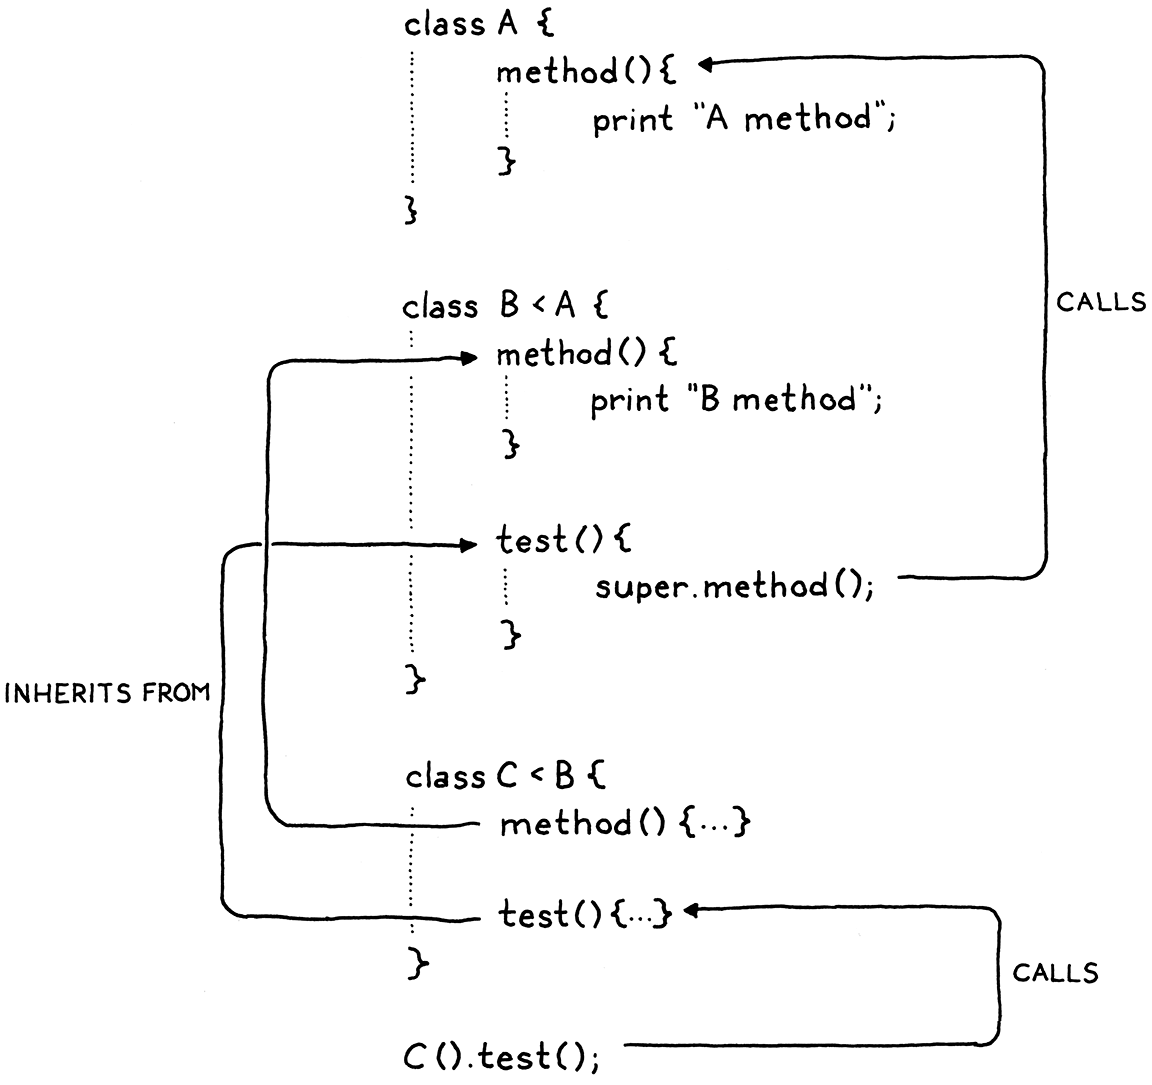
\includegraphics[width=\textwidth]{image/inheritance/classes.png}
\end{figure}

因此,为了对super表达式求值,我们需要访问围绕方法调用的类的超类。可惜的是,在解释器中执行super表达式的地方,我们并没有那么容易获得。

我们可以从LoxFunction添加一个字段,以存储指向拥有该方法的LoxClass的引用。解释器会保存执行当前执行的LoxFunction的引用,这样稍后在遇到super表达式时就可以找到它。从它开始,可以得到方法的LoxClass,然后找到它的超类。

这需要很多管道。在上一章中,我们添加对this的支持时遇到了类似的问题。在那种情况下,我们使用已有的环境和闭包机制保存了指向当前对象的引用。那我们是否可以做类似的事情来存储超类?嗯,如果答案是否定的,我就不会问这个问题了,所以...是的。

一个重要的区别是,我们在方法被访问时绑定了this。同一个方法可以在不同的实例上被调用,而且每个实例都需要有自己的this。对于super表达式,超类是\textit{类声明本身}的一个固定属性。每次对某个super表达式求值时,超类都是同一个。

这意味着我们可以在执行类定义时,为超类创建一个环境。在定义方法之前,我们创建一个新环境,将类的超类与名称super绑定。

\begin{figure}[htbp]
  \centering
  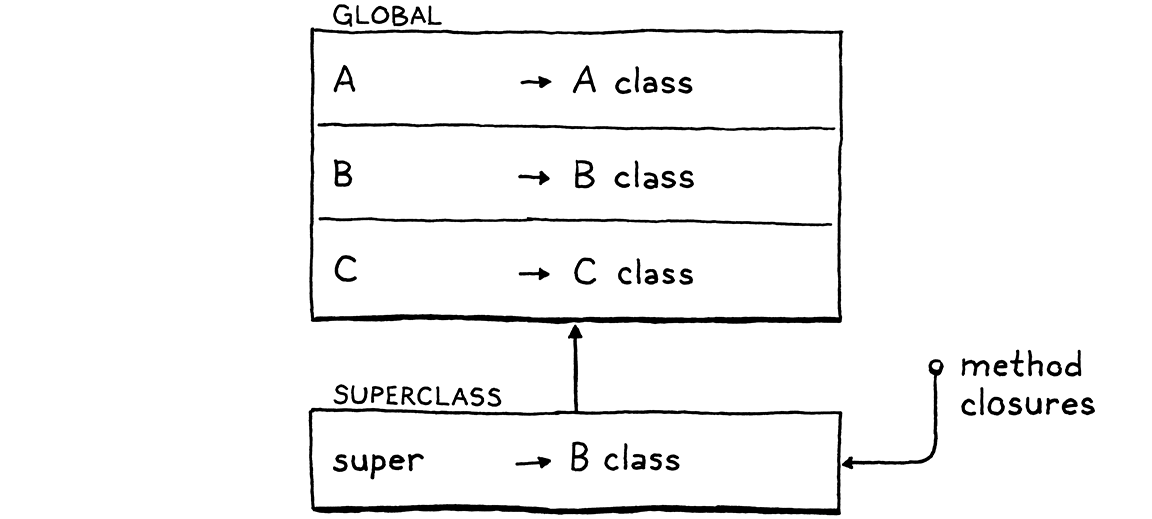
\includegraphics[width=\textwidth]{image/inheritance/superclass.png}
\end{figure}

当我们为每个方法创建LoxFunction运行时表示时,也就是这个方法闭包中获取的环境。之后,放方法被调用时会绑定this,超类环境会成为方法环境的父环境,就像这样:

\begin{figure}[htbp]
  \centering
  \includegraphics[width=\textwidth]{image/inheritance/environments.png}
\end{figure}

这是一个复杂的机制,但是我们会一步一步完成它。在我们可以在运行时创建环境之前,我们需要在分析器中处理对应的作用域。

\begin{code}{java}{3-6}{lox/Resolver.java,在visitClassStmt()方法中添加}
      resolve(stmt.superclass);
    }
    if (stmt.superclass != null) {
      beginScope();
      scopes.peek().put("super", true);
    }
    beginScope();
\end{code}

如果该类声明有超类,那么我们就在其所有方法的外围创建一个新的作用域。在这个作用域中,我们会定义名称super。一旦我们完成了对该类中方法的分析,就丢弃这个作用域。

\begin{code}{java}{2}{lox/Resolver.java,在visitClassStmt()方法中添加}
    endScope();
    if (stmt.superclass != null) endScope();
    currentClass = enclosingClass;
\end{code}

这是一个小优化,但是我们只在类真的有超类时才会创建超类环境。在没有超类的情况下,创建超类环境是没有意义的,因为无论如何里面都不会存储超类。

在作用域链中定义super后,我们就能够分析super表达式了。

\begin{code}{java}{}{lox/Resolver.java,在visitSetExpr()方法后添加}
  @Override
  public Void visitSuperExpr(Expr.Super expr) {
    resolveLocal(expr, expr.keyword);
    return null;
  }
\end{code}

我们把super标记当作一个变量进行分析。分析结果保存了解释器要在环境链上找到超类所在的环境需要的跳数。

这段代码在解释器中也有对应。当我们执行子类定义时,创建一个新环境。

\begin{code}{java}{7-10}{lox/Interpreter.java,在visitClassStmt()方法中添加}
        throw new RuntimeError(stmt.superclass.name,
            "Superclass must be a class.");
      }
    }

    environment.define(stmt.name.lexeme, null);
    if (stmt.superclass != null) {
      environment = new Environment(environment);
      environment.define("super", superclass);
    }
    Map<String, LoxFunction> methods = new HashMap<>();
\end{code}

在这个环境中,我们保存指向超类的引用——即我们在运行时现在拥有的超类的实际LoxClass对象。然后我们为每个方法创建LoxFunction。这些函数将捕获当前环境(也就是我们刚刚绑定“super”的那个)作为其闭包,像我们需要的那样维系着超类。一旦这些完成,我们就弹出环境。

\begin{code}{java}{3-5}{lox/Interpreter.java,在visitClassStmt()方法中添加}
    LoxClass klass = new LoxClass(stmt.name.lexeme,
        (LoxClass)superclass, methods);
    if (superclass != null) {
      environment = environment.enclosing;
    }
    environment.assign(stmt.name, klass);
\end{code}

我们现在已经准备好解释super表达式了。这会分为很多部分,所以我们逐步构建这个方法。

\begin{code}{java}{}{lox/Interpreter.java,在visitSetExpr()方法后添加}
  @Override
  public Object visitSuperExpr(Expr.Super expr) {
    int distance = locals.get(expr);
    LoxClass superclass = (LoxClass)environment.getAt(
        distance, "super");
  }
\end{code}

首先,我们要做之前铺垫的工作。我们通过在适当环境中查找“super”来找到外围类的超类。

当我们访问方法时,还需要将this与访问该方法的对象进行绑定。在像doughnut.cook这样的表达式中,对象是我们通过对doughnut求值得到的内容。在像super.cook这样的super表达式中,当前对象隐式地与我们正使用的当前对象相同。换句话说,就是this。即使我们在超类中查找方法,\textit{实例}仍然是this。

不幸的是,在super表达式中,我们没有一个方便的节点可以让分析器将this对应的跳数保存起来。幸运的是,我们可以控制环境链的布局。绑定this的环境总是存储在保存super的环境中。

\begin{code}{java}{3-4}{lox/Interpreter.java,在visitSuperExpr()方法中添加}
    LoxClass superclass = (LoxClass)environment.getAt(
        distance, "super");
    LoxInstance object = (LoxInstance)environment.getAt(
        distance - 1, "this");
  }
\end{code}

将距离偏移1,在那个内部环境中查找“this”。我承认中国代码不是最优雅的,但是它是有效的。

现在我们准备查找并绑定方法,从超类开始。

\begin{code}{java}{3-5}{lox/Interpreter.java,在visitSuperExpr()方法中添加}
    LoxInstance object = (LoxInstance)environment.getAt(
        distance - 1, "this");
    LoxFunction method = superclass.findMethod(expr.method.lexeme);
    return method.bind(object);
  }
\end{code}

这几乎与查找get表达式方法的代码完全一样,区别在于,我们是在超类上调用findMethod() ,而不是在当前对象的类。

基本上就是这样了。当然,除了我们可能找不到方法之外。所以,我们要对其检查。

\begin{code}{java}{2-5}{lox/Interpreter.java,在visitSuperExpr()方法中添加}
    LoxFunction method = superclass.findMethod(expr.method.lexeme);
    if (method == null) {
      throw new RuntimeError(expr.method,
          "Undefined property '" + expr.method.lexeme + "'.");
    }
    return method.bind(object);
  }
\end{code}

这就对了!试着运行一下前面那个BostonCream的例子。如果你我都做对了,它的结果应该是:

\begin{code}{js}{}{}
Fry until golden brown.
Pipe full of custard and coat with chocolate.
\end{code}

\subsection{super的无效使用}

像以前的语言特性一样,当用户写出正确的代码时,我们的语言实现也会做成正确的事情,但我们还没有在解释器中对错误代码进行防御。具体来说,考虑以下代码:

\begin{code}{java}{}{}
class Eclair {
  cook() {
    super.cook();
    print "Pipe full of crème pâtissière.";
  }
}
\end{code}

这个类中有一个super表达式,但是没有超类。在运行时,计算super表达式的代码假定super已经被成功分析,并且可以在环境中找到超类。但是在这里会失败,因为没有超类,也就没有超类对应的外围环境。JVM会抛出一个异常,我们的解释器也会因此崩溃。

见鬼,还有更简单的super错误用法:

\begin{code}{java}{}{}
super.notEvenInAClass();
\end{code}

我们可以在运行时通过检查“super”是否查找成功而处理此类错误。但是我们可以只通过查看源代码静态地知道,Eclair没有超类,因此也就没有super表达式可以在其中生效。同样的,在第二个例子中,我们知道super表达式甚至不在方法体内。

尽管Lox是动态类型的,但这并不意味着我们要将一切都推迟到运行时。如果用户犯了错误,我们希望能帮助他们尽早发现,所以我们会在分析器中静态地报告这些错误。

首先,在我们用来追踪当前访问代码外围类的类型的枚举中添加一个新值。

\begin{code}{java}{3}{lox/Resolver.java,在ClassType枚举中添加代码,首先在上一行后面加“,”:}
    NONE,
    CLASS,
    SUBCLASS
  }
\end{code}

我们将用它来区分我们是否在一个由超类的类中。当我们分析一个类的声明时,如果该类是一个子类,我们就设置该值。

\begin{code}{java}{2}{lox/Resolver.java,在visitClassStmt()方法中添加}
    if (stmt.superclass != null) {
      currentClass = ClassType.SUBCLASS;
      resolve(stmt.superclass);
\end{code}

然后,当我们分析super表达式时,会检查当前是否在一个允许使用super表达式的作用域中。

\begin{code}{java}{2-8}{lox/Resolver.java,在visitSuperExpr()方法中添加}
  public Void visitSuperExpr(Expr.Super expr) {
    if (currentClass == ClassType.NONE) {
      Lox.error(expr.keyword,
          "Can't use 'super' outside of a class.");
    } else if (currentClass != ClassType.SUBCLASS) {
      Lox.error(expr.keyword,
          "Can't use 'super' in a class with no superclass.");
    }
    resolveLocal(expr, expr.keyword);
\end{code}

如果不是,那就是用户出错了。

\section{总结}

我们成功了!最后的错误处理是完成Lox语言的Java实现所需的最后一块代码。这是一项真正的成就,你应该为此感到自豪。在过去的十几章和一千多行代码中,我们已经学习并实现了:

\begin{itemize}
  \item 标记与词法
  \item 抽象语法树
  \item 递归下降分析
  \item 前缀、中缀表达式
  \item 对象的运行时表示
  \item 使用Visitor模式解释代码
  \item 词法作用域
  \item 保存变量的环境链
  \item 控制流
  \item 有参函数
  \item 闭包
  \item 静态变量分析与错误检查
  \item 类
  \item 构造函数
  \item 字段
  \item 方法
  \item 继承
\end{itemize}

所有这些都是我们从头开始做的,没有借助外部依赖和神奇工具。只有你和我,我们的文本编辑器,Java标准库中的几个集合类,以及JVM运行时。

这标志着第二部分的结束,但不是这本书的结束。休息一下,也许可以编写几个Lox程序在你的解释器中运行一下(你可能需要添加一些本地方法来支持读取用户的输入等操作)。当你重新振作之后,我们将开始下一次冒险。

\section{挑战}

\begin{enumerate}
\item Lox只支持\textit{单继承}——一个类可以有一个超类,这是唯一跨类复用方法的方式。其它语言中已经探索出了各种方法来更自由地跨类重用和共享功能:mixins, traits, multiple inheritance, virtual inheritance, extension methods, 等等。

   如果你要在Lox中添加一些类似的功能,你会选择哪种,为什么?如果你有勇气的话(这时候你应该有勇气了),那就去添加它。

\item 在Lox中,与其它大多数面向对象语言一样,当查找一个方法时,我们从类的底层开始向上查找——子类的方法优先于超类的方法。为了在覆盖方法中访问超类方法,你可以使用super。

   BEAT语言采用了相反的方法。当你调用一个方法时,它从类继承结构的顶层开始向下寻找。超类方法的优先级高于子类方法。为了访问子类的方法,超类方法可以调用inner,这有点像是super的反义词。它与继承层次结构中的下一级方法相连接。

   超类方法控制着子类何时何地可以改进其行为。如果超类方法根本没有调用inner,那么子类就无法覆盖或修改超类的行为。

   去掉Lox目前的覆盖和super行为,用BEAT的语义来替换。简而言之:
  
  \begin{itemize}
    \item 当调用类上的方法时,优先选择类继承链中最高的方法。
    \item 在方法体内部,inner调用会在继承链中包含inner的类和包含this的类之间,查找具有相同名称的最近的子类中的方法。如果没有匹配的方法,inner调用不做任何事情。
  \end{itemize}

   举例来说:

   \begin{code}{java}{}{}
   class Doughnut {
     cook() {
       print "Fry until golden brown.";
       inner();
       print "Place in a nice box.";
     }
   }
   
   class BostonCream < Doughnut {
     cook() {
       print "Pipe full of custard and coat with chocolate.";
     }
   }
   
   BostonCream().cook();
   \end{code}

   这应该输出:

   \begin{code}{js}{}{}
   Fry until golden brown.
   Pipe full of custard and coat with chocolate.
   Place in a nice box.
   \end{code}

\item 在介绍Lox的那一章,我让你想出几个你认为该语言缺少的功能。现在你知道了如何构建一个解释器,请实现其中的一个功能。
\end{enumerate}

\part{字节码虚拟机}

我们的Java解释器jlox教会了我们许多编程语言的基础知识,但我们仍然有许多东西需要学习。首先,如果你在jlox中运行任何Lox程序,你会发现它非常慢。它所使用的解释方式——直接遍历AST,对于某些实际应用来说已经足够了,但是对于通用脚本语言来说还有很多不足之处。

另外,我们隐式地依赖于JVM本身的运行时特性。我们想当然地认为像instanceof这样的语句在Java中是可以工作的。而且我们从未担心过内存管理,因为JVM的垃圾收集器为我们解决了这个问题。

当我们专注于高层次概念时,我们可以忽略这些。但现在我们已经对解释器了如指掌,是时候深入到这些底层,从头开始构建我们自己的虚拟机,只用C语言标准库就可以了……

\chapter{字节码块}

\epigraph{如果你发现你几乎把所有的时间都花在了理论上,那就开始把一些注意力转向实际的东西;这会提高你的理论水平。如果你发现你几乎把所有的时间都花在了实践上,那就开始把一些注意力转向理论上的东西;这将改善你的实践。}{高德纳}

我们已经有了一个Lox的完整实现jlox,那么为什么这本书还没有结束呢?部分原因是jlox依赖JVM为我们做很多事情。如果我们想要了解一个解释器是如何工作的,我们就需要自己构建这些零碎的东西。

jlox不够用的一个更根本的原因在于,它太慢了。树遍历解释器对于某些高级的声明式语言来说是不错的,但是对于通用的命令式语言——即使是Lox这样的“脚本”语言——这是行不通的。以下面的小脚本为例:

\begin{code}{js}{}{}
fun fib(n) {
  if (n < 2) return n;
  return fib(n - 1) + fib(n - 2); 
}

var before = clock();
print fib(40);
var after = clock();
print after - before;
\end{code}

在我们的笔记本电脑上,jlox大概需要72秒的时间来执行。一个等价的C程序在半秒内可以完成。我们的动态类型的脚本语言永远不可能像手动管理内存的静态类型语言那样快,但我们没必要满足于慢两个数量级以上的速度。

我们可以把jlox放在性能分析器中运行,并进行调优和调整热点,但这也只能到此为止了。它的执行模型(遍历AST)从根本上说就是一个错误的设计。我们无法将其微优化到我们想要的性能,就像你无法将AMC Gremlin打磨成SR-71 Blackbird一样。

我们需要重新考虑核心模型。本章将介绍这个模型——字节码,并开始我们的新解释器,clox。

\section{字节码?}

在工程领域,很少有选择是不需要权衡的。为了更好地理解我们为什么要使用字节码,让我们将它与几个备选方案进行比较。

\subsection{为什么不遍历AST?}

我们目前的解释器有几个优点:

\begin{itemize}
  \item 嗯,首先我们已经写好了,它已经完成了。它能完成的主要原因是这种风格的解释器\textit{实现起来非常简单}。代码的运行时表示直接映射到语法。从解析器到我们在运行时需要的数据结构,几乎都毫不费力。
  \item 它是可移植的。我们目前的解释器是使用Java编写的,可以在Java支持的任何平台上运行。我们可以用同样的方法在C语言中编写一个新的实现,并在世界上几乎所有平台上编译并运行我们的语言。
\end{itemize}

这些是真正的优势。但是,另一方面,它的内存使用效率不高。每一段语法都会变成一个AST节点。像1+2这样的Lox表达式会变成一连串的对象,对象之间有很多指针,就像:

\begin{figure}[htbp]
  \centering
  \includegraphics[width=\textwidth]{image/chunks-of-bytecode/ast.png}
\end{figure}

每个指针都会给对象增加32或64比特的开销。更糟糕的是,将我们的数据散布在一个松散连接的对象网络中的堆上,会对空间局部性造成影响。

现代CPU处理数据的速度远远超过它们从RAM中提取数据的速度。为了弥补这一点,芯片中有多层缓存。如果它需要的一块存储数据已经在缓存中,它就可以更快地被加载。我们谈论的是100倍以上的提速。

数据是如何进入缓存的?机器会推测性地为你把数据塞进去。它的启发式方法很简单。每当CPU从RAM中读取数据时,它就会拉取一块相邻的字节并放到缓存中。

如果我们的程序接下来请求一些在缓存行中的数据,那么我们的CPU就能像工厂里一条运转良好的传送带一样运行。我们真的很想利用这一点。为了有效的利用缓存,我们在内存中表示代码的方式应该像读取时一样紧密而有序。

现在抬头看看那棵树。这些子对象可能在任何地方。树遍历器的每一步都会引用子节点,都可能会超出缓存的范围,并迫使CPU暂停,直到从RAM中拉取到新的数据块(才会继续执行)。仅仅是这些树形节点及其所有指针字段和对象头的开销,就会把对象彼此推离,并将其推出缓存区。

我们的AST遍历器在接口调度和Visitor模式方面还有其它开销,但仅仅是局部性问题就足以证明使用更好的代码表示是合理的。

\subsection{为什么不编译成本地代码?}

如果你想真正快,就要摆脱所有的中间层,一直到最底层——机器码。听起来就很快,\textit{机器码}。

最快的语言所做的是直接把代码编译为芯片支持的本地指令集。从早期工程师真正用机器码手写程序以来,以本地代码为目标一直是最有效的选择。

如果你以前从来没有写过任何机器码,或者是它略微讨人喜欢的近亲汇编语言,那我给你做一个简单的介绍。本地代码是一系列密集的操作,直接用二进制编码。每条指令的长度都在一到几个字节之间,而且几乎是令人头疼的底层指令。“将一个值从这个地址移动到这个寄存器”“将这两个寄存器中的整数相加”,诸如此类。

通过解码和按顺序执行指令来操作CPU。没有像AST那样的树状结构,控制流是通过从代码中的一个点跳到另一个点来实现的。没有中间层,没有开销,没有不必要的跳转或指针寻址。

闪电般的速度,但这种性能是有代价的。首先,编译成本地代码并不容易。如今广泛使用的大多数芯片都有着庞大的拜占庭式架构,其中包含了几十年来积累的大量指令。它们需要复杂的寄存器分配、流水线和指令调度。

当然,你可以把可移植性抛在一边。花费几年时间掌握一些架构,但这仍然只能让你接触到一些流行的指令集。为了让你的语言能在所有的架构上运行,你需要学习所有的指令集,并为每个指令集编写一个单独的后端。

\subsection{什么是字节码?}

记住这两点。一方面,树遍历解释器简单、可移植,而且慢。另一方面,本地代码复杂且特定与平台,但是很快。字节码位于中间。它保留了树遍历型的可移植性——在本书中我们不会编写汇编代码,同时它牺牲了一些简单性来换取性能的提升,虽然没有完全的本地代码那么快。

结构上讲,字节码类似于机器码。它是一个密集的、线性的二进制指令序列。这样可以保持较低的开销,并可以与高速缓存配合得很好。然而,它是一个更简单、更高级的指令集,比任何真正的芯片都要简单。(在很多字节码格式中,每条指令只有一个字节长,因此称为“字节码”)

想象一下,你在用某种源语言编写一个本地编译器,并且你可以全权定义一个尽可能简单的目标架构。字节码就有点像这样,它是一个理想化的幻想指令集,可以让你作为编译器作者的生活更轻松。

当然,幻想架构的问题在于它并不存在。我们提供编写模拟器来解决这个问题,这个模拟器是一个用软件编写的芯片,每次会解释字节码的一条指令。如果你愿意的话,可以叫它\textit{虚拟机(VM)}。

模拟层增加了开销,这是字节码比本地代码慢的一个关键原因。但作为回报,它为我们提供了可移植性。用像C这样的语言来编写我们的虚拟机,它已经被我们所关心的所有机器所支持,这样我们就可以在任何我们喜欢的硬件上运行我们的模拟器。

这就是我们的新解释器clox要走的路。我们将追随Python、Ruby、Lua、OCaml、Erlang和其它主要语言实现的脚步。在许多方面,我们的VM设计将与之前的解释器结构并行。

\begin{figure}[htbp]
  \centering
  \includegraphics[width=\textwidth]{image/chunks-of-bytecode/phases.png}
\end{figure}

当然,我们不会严格按照顺序实现这些阶段。像我们之前的解释器一样,我们会反复地构建实现,每次只构建一种语言特性。在这一章中,我们将了解应用程序的框架,并创建用于存储和表示字节码块的数据结构。

\section{开始}

除了main()还能从哪里开始呢?启动你的文本编辑器,开始输入。

\begin{code}{c}{}{创建新文件main.c}
#include "common.h"

int main(int argc, const char* argv[]) {
  return 0;
}
\end{code}

从这颗小小的种子开始,我们将成长为整个VM。由于C提供给我们的东西太少,我们首先需要花费一些时间来培育土壤。其中一部分就在下面的header中。

\begin{code}{c}{}{创建新文件common.h}
#ifndef clox_common_h
#define clox_common_h

#include <stdbool.h>
#include <stddef.h>
#include <stdint.h>

#endif
\end{code}

在整个解释器中,我们会使用一些类型和常量,这是一个方便放置它们的地方。现在,它是古老的NULL、size\_t,C99中的布尔类型bool,以及显式声明大小的整数类型——uint8\_t和它的朋友们。

\section{指令块}

接下来,我们需要一个模块来定义我们的代码表示形式。我一直使用“chunk”指代字节码序列,所以我们把它作为该模块的正式名称。

\begin{code}{c}{}{创建新文件chunk.h}
#ifndef clox_chunk_h
#define clox_chunk_h

#include "common.h"

#endif
\end{code}

在我们的字节码格式中,每个指令都有一个字节的\textbf{操作码}(通常简称为\textbf{opcode})。这个数字控制我们要处理的指令类型——加、减、查找变量等。我们在这块定义这些:

\begin{code}{c}{2-4}{chunk.h,添加代码}
#include "common.h"
typedef enum {
  OP_RETURN,
} OpCode;
#endif
\end{code}

现在,我们从一条指令OP\_RETURN开始。当我们有一个全功能的VM时,这个指令意味着“从当前函数返回”。我承认这还不是完全有用,但是我们必须从某个地方开始下手,而这是一个特别简单的指令,原因我们会在后面讲到。

\subsection{指令动态数组}

字节码是一系列指令。最终,我们会与指令一起存储一些其它数据,所以让我们继续创建一个结构体来保存所有这些数据。

\begin{code}{c}{2-4}{chunk.h,在枚举OpCode后添加}
} OpCode;
typedef struct {
  uint8_t* code;
} Chunk;
#endif
\end{code}

目前,这只是一个字节数组的简单包装。由于我们在开始编译块之前不知道数组需要多大,所以它必须是动态的。动态数组是我最喜欢的数据结构之一。这听起来就像是在说香草是我最喜爱的冰淇淋口味,但请听我说完。动态数组提供了:

\begin{itemize}
  \item 缓存友好,密集存储
  \item 索引元素查找为常量时间复杂度
  \item 数组末尾追加元素为常量时间复杂度
\end{itemize}

这些特性正是我们在jlox中以ArrayList类的名义一直使用动态数组的原因。现在我们在C语言中,可以推出我们自己的动态数组。如果你对动态数组不熟悉,其实这个想法非常简单。除了数组本身,我们还保留了两个数字:数组中已分配的元素数量(容量,capacity)和实际使用的已分配元数数量(计数,count)。

\begin{code}{c}{2-3}{chunk.h,在结构体Chunk中添加代码}
typedef struct {
  int count;
  int capacity;
  uint8_t* code;
} Chunk;
\end{code}

当添加元素时,如果计数小于容量,那么数组中已有可用空间。我们将新元素直接存入其中,并修改计数值。

\begin{figure}[htbp]
  \centering
  \includegraphics[width=\textwidth]{image/chunks-of-bytecode/insert.png}
\end{figure}

如果没有多余的容量,那么这个过程会稍微复杂一些。

\begin{figure}[htbp]
  \centering
  \includegraphics[width=\textwidth]{image/chunks-of-bytecode/grow.png}
\end{figure}

\begin{enumerate}
  \item 分配一个容量更大的新数组。
  \item 将旧数组中的已有元素复制到新数组中。
  \item 保存新的capacity。
  \item 删除旧数组。
  \item 更新code指向新的数组。
  \item 现在有了空间,将元素存储在新数组中。
  \item 更新count。
\end{enumerate}

我们的结构体已经就绪,现在我们来实现使用它的函数。C语言没有构造函数,所以我们声明一个函数来初始化一个新的块。

\begin{code}{c}{2}{chunk.h,在结构体Chunk后添加}
} Chunk;
void initChunk(Chunk* chunk);
#endif
\end{code}

并这样实现它:

\begin{code}{c}{}{chunk.c,创建新文件}
#include <stdlib.h>

#include "chunk.h"

void initChunk(Chunk* chunk) {
  chunk->count = 0;
  chunk->capacity = 0;
  chunk->code = NULL;
}
\end{code}

动态数组一开始是完全空的。我们甚至还没有分配原始数组。要将一个字节追加到块的末尾,我们使用一个新函数。

\begin{code}{c}{2}{chunk.h,在initChunk()方法后添加}
void initChunk(Chunk* chunk);
void writeChunk(Chunk* chunk, uint8_t byte);
#endif
\end{code}

这就是有趣的地方。

\begin{code}{c}{}{chunk.c,在initChunk()方法后添加}
void writeChunk(Chunk* chunk, uint8_t byte) {
  if (chunk->capacity < chunk->count + 1) {
    int oldCapacity = chunk->capacity;
    chunk->capacity = GROW_CAPACITY(oldCapacity);
    chunk->code = GROW_ARRAY(uint8_t, chunk->code,
        oldCapacity, chunk->capacity);
  }

  chunk->code[chunk->count] = byte;
  chunk->count++;
}
\end{code}

我们需要做的第一件事是查看当前数组是否已经有容纳新字节的容量。如果没有,那么我们首先需要扩充数组以腾出空间(当我们第一个写入时,数组为NULL并且capacity为0,也会遇到这种情况)

要扩充数组,首先我们要算出新容量,然后将数组容量扩充到该大小。这两种低级别的内存操作都在一个新模块中定义。

\begin{code}{c}{2}{chunk.c,添加代码}
#include "chunk.h"
#include "memory.h"
void initChunk(Chunk* chunk) {
\end{code}

这就足够我们开始后面的事情了。

\begin{code}{c}{}{memory.h,创建新文件}
#ifndef clox_memory_h
#define clox_memory_h

#include "common.h"

#define GROW_CAPACITY(capacity) \
    ((capacity) < 8 ? 8 : (capacity) * 2)

#endif
\end{code}

这个宏会根据给定的当前容量计算出新的容量。为了获得我们想要的性能,重要的部分就是基于旧容量大小进行扩展。我们以2的系数增长,这是一个典型的取值。1.5是另外一个常见的选择。

我们还会处理当前容量为0的情况。在这种情况下,我们的容量直接跳到8,而不是从1开始。这就避免了在数组非常小的时候出现额外的内存波动,代价是在非常小的块中浪费几个字节。

一旦我们知道了所需的容量,就可以使用GROW\_ARRAY()创建或扩充数组到该大小。

\begin{code}{c}{2-6}{memory.h,添加代码}
#define GROW_CAPACITY(capacity) ((capacity) < 8 ? 8 : (capacity) * 2)
#define GROW_ARRAY(type, pointer, oldCount, newCount) \
    (type*)reallocate(pointer, sizeof(type) * (oldCount), \
        sizeof(type) * (newCount))

void* reallocate(void* pointer, size_t oldSize, size_t newSize);
#endif
\end{code}

这个宏简化了对reallocate()函数的调用,真正的工作就是在其中完成的。宏本身负责获取数组元素类型的大小,并将生成的void*转换成正确类型的指针。

这个reallocate()函数是我们将在clox中用于所有动态内存管理的唯一函数——分配内存,释放内存以及改变现有分配的大小。当我们稍后添加一个需要跟踪内存使用情况的垃圾收集器时,通过单个函数路由所有这些操作是很重要的。

传递给reallocate()函数的两个大小参数控制了要执行的操作:

\begin{center}
  \begin{tabular}{ |c|c|c| } 
   \hline
   oldSize & newSize & 操作 \\
   \hline 
   0 & 非0 & 分配新块 \\ 
   非0 & 0 & 释放已分配内存 \\
   非0 & 小于oldSize & 收缩已分配内存 \\
   非0 & 大于newSize & 增加已分配内存 \\
   \hline
  \end{tabular}
\end{center}

看起来好像有很多情况需要处理,但下面是其实现:

\begin{code}{c}{}{memory.c,创建新文件}
#include <stdlib.h>

#include "memory.h"

void* reallocate(void* pointer, size_t oldSize, size_t newSize) {
  if (newSize == 0) {
    free(pointer);
    return NULL;
  }

  void* result = realloc(pointer, newSize);
  return result;
}
\end{code}

当newSize为0时,我们通过调用free()来自己处理回收的情况。其它情况下,我们依赖于C标准库的realloc()函数。该函数可以方便地支持我们策略中的其它三个场景。当oldSize为0时,realloc()等同于调用malloc()。

有趣的情况是当oldSize和newSize都不为0时。它们会告诉realloc()要调整之前分配的块的大小。如果新的大小小于现有的内存块,它就只是更新块的大小,并返回传入的指针。如果新块大小更大,它就会尝试增长现有的内存块。

只有在该块之后的内存未被使用的情况下,才能这样做。如果没有空间支持块的增长,realloc()会分配一个所需大小的\textit{新}的内存块,复制旧的字节,释放旧内存块,然后返回一个指向新内存块的指针。记住,这正是我们的动态数组想要的行为。

因为计算机是有限的物质块,而不是计算机科学理论所认为的完美的数学抽象,如果没有足够的内存,分配就会失败,reealloc()会返回NULL。我们应该解决这个问题。

\begin{code}{c}{2}{memory.c,在reallocate()方法中添加}
  void* result = realloc(pointer, newSize);
  if (result == NULL) exit(1);
  return result;
\end{code}

如果我们的VM不能得到它所需要的内存,那就做不了什么有用的事情,但我们至少可以检测这一点,并立即中止进程,而不是返回一个NULL指针,然后让程序运行偏离轨道。

好了,我们可以创建新的块并向其中写入指令。我们完成了吗?不!要记住,我们现在是在C语言中,我们必须自己管理内存,就像在《Ye Olden Times》中那样,这意味着我们也要\textit{释放}内存。

\begin{code}{c}{2}{chunk.h,在initChunk()方法后添加}
void initChunk(Chunk* chunk);
void freeChunk(Chunk* chunk);
void writeChunk(Chunk* chunk, uint8_t byte);
\end{code}

实现为:

\begin{code}{c}{}{chunk.c,在initChunk()方法后添加}
void freeChunk(Chunk* chunk) {
  FREE_ARRAY(uint8_t, chunk->code, chunk->capacity);
  initChunk(chunk);
}
\end{code}

我们释放所有的内存,然后调用initChunk()将字段清零,使字节码块处于一个定义明确的空状态。为了释放内存,我们再添加一个宏。

\begin{code}{c}{4-5}{memory.h,添加代码}
#define GROW_ARRAY(type, pointer, oldCount, newCount) \
    (type*)reallocate(pointer, sizeof(type) * (oldCount), \
        sizeof(type) * (newCount))
#define FREE_ARRAY(type, pointer, oldCount) \
    reallocate(pointer, sizeof(type) * (oldCount), 0)
void* reallocate(void* pointer, size_t oldSize, size_t newSize);
\end{code}

与GROW\_ARRAY()类似,这是对reallocate()调用的包装。这个函数通过传入0作为新的内存块大小,来释放内存。我知道,这是一堆无聊的低级别代码。别担心,在后面的章节中,我们会大量使用这些内容。但在此之前,我们必须先打好自己的基础。

\section{反汇编字节码块}

现在我们有一个创建字节码块的小模块。让我们手动构建一个样例字节码块来测试一下。

\begin{code}{c}{2-5}{main.c,在main()方法中添加}
int main(int argc, const char* argv[]) {
  Chunk chunk;
  initChunk(&chunk);
  writeChunk(&chunk, OP_RETURN);
  freeChunk(&chunk);
  return 0;
\end{code}

不要忘了include。

\begin{code}{c}{2}{main.c,添加代码}
#include "common.h"
#include "chunk.h"
int main(int argc, const char* argv[]) {
\end{code}

试着运行一下,它起作用了吗?额...谁知道呢。我们所做的只是在内存中存入一些字节。我们没有人性化的方法来查看我们制作的字节码块中到底有什么。

为了解决这个问题,我们要创建一个\textbf{反汇编程序}。\textbf{汇编程序}是一个老式程序,它接收一个文件,该文件中包含CPU指令(如“ADD”和“MULT”)的可读助记符名称,并将它们翻译成等价的二进制机器代码。反汇编程序则相反——给定一串机器码,它会返回指令的文本列表。

我们将实现一个类似的模块。给定一个字节码块,它将打印出其中所有的指令。Lox用户不会使用它,但我们这些Lox的维护者肯定会从中受益,因为它给我们提供了一个了解解释器内部代码表示的窗口。

在main()中,我们创建字节码块后,将其传入反汇编器。

\begin{code}{c}{3}{main.c,在main()方法中添加}
  initChunk(&chunk);
  writeChunk(&chunk, OP_RETURN);
  disassembleChunk(&chunk, "test chunk");
  freeChunk(&chunk);
\end{code}

我们又创建了另一个模块。

\begin{code}{c}{2}{main.c,添加代码}
#include "chunk.h"
#include "debug.h"
int main(int argc, const char* argv[]) {
\end{code}

下面是这个头文件:

\begin{code}{c}{}{debug.h,创建新文件}
#ifndef clox_debug_h
#define clox_debug_h

#include "chunk.h"

void disassembleChunk(Chunk* chunk, const char* name);
int disassembleInstruction(Chunk* chunk, int offset);

#endif
\end{code}

在main()方法中,我们调用disassembleChunk()来反汇编整个字节码块中的所有指令。这是用另一个函数实现的,该函数只反汇编一条指令。因为我们将在后面的章节中从VM中调用它,所以将它添加到头文件中。

下面是简单的实现文件:

\begin{code}{c}{}{debug.c,创建新文件}
#include <stdio.h>

#include "debug.h"

void disassembleChunk(Chunk* chunk, const char* name) {
  printf("== %s ==\n", name);

  for (int offset = 0; offset < chunk->count;) {
    offset = disassembleInstruction(chunk, offset);
  }
}
\end{code}

要反汇编一个字节码块,我们首先打印一个小标题(这样我们就知道正在看哪个字节码块),然后通过字节码反汇编每个指令。我们遍历代码的方式有点奇怪。我们没有在循环中增加offset,而是让disassembleInstruction()为我们做这个。当我们调用该函数时,在对给定偏移量的位置反汇编指令后,会返回\textit{下一条}指令的偏移量。这是因为,我们后面也会看到,指令可以有不同的大小。

“debug”模块的核心是这个函数:

\begin{code}{c}{}{debug.c,在disassembleChunk()方法后添加}
int disassembleInstruction(Chunk* chunk, int offset) {
  printf("%04d ", offset);

  uint8_t instruction = chunk->code[offset];
  switch (instruction) {
    case OP_RETURN:
      return simpleInstruction("OP_RETURN", offset);
    default:
      printf("Unknown opcode %d\n", instruction);
      return offset + 1;
  }
}
\end{code}

首先,它会打印给定指令的字节偏移量——这能告诉我们当前指令在字节码块中的位置。当我们在字节码中实现控制流和跳转时,这将是一个有用的路标。

接下来,它从字节码中的给定偏移量处读取一个字节。这也就是我们的操作码。我们根据该值做switch操作。对于每一种指令,我们都分派给一个小的工具函数来展示它。如果给定的字节看起来根本不像一条指令——这是我们编译器的一个错误——我们也要打印出来。对于我们目前仅有的一条指令OP\_RETURN,对应的展示函数是:

\begin{code}{c}{}{debug.c,在disassembleChunk()方法后添加}
static int simpleInstruction(const char* name, int offset) {
  printf("%s\n", name);
  return offset + 1;
}
\end{code}

return指令的内容不多,所以它所做的只是打印操作码的名称,然后返回该指令后的下一个字节偏移量。其它指令会有更多的内容。

如果我们现在运行我们的新解释器,它实际上会打印出来:

\begin{code}{js}{}{}
== test chunk ==
0000 OP_RETURN
\end{code}

成功了!这有点像我们代码表示中的“Hello, world!”。我们可以创建一个字节码块,向其中写入一条指令,然后将该指令提取出来。我们对二进制字节码的编码和解码工作正常。

\section{常量}

现在我们有了一个基本的块结构,我们来让它变得更有用。我们可以在块中存储\textit{代码},但是\textit{数据}呢?解释器中使用的很多值都是在运行时作为操作的结果创建的。

\begin{code}{js}{}{}
1 + 2;
\end{code}

这里的代码中没有出现3这个值。但是,字面量1和2出现了。为了将该语句编译成字节码,我们需要某种指令,其含义是“生成一个常量”,而这些字母值需要存储在字节码块中的某个地方。在jlox中,Expr.Literal这个AST节点中保存了这些值。因为我们没有语法树,现在我们需要一个不同的解决方案。

\subsection{表示值}

在本章中我们不会运行任何代码,但是由于常量在解释器的静态和动态世界中都有涉足,这会迫使我们开始思考我们的虚拟机中应该如何表示数值。

现在,我们尽可能从最简单的开始——只支持双精度浮点数。这种表示形式显然会逐渐扩大,所以我们将建立一个新的模块,给自己留出扩展的空间。

\begin{code}{c}{}{value.h,创建新文件}
#ifndef clox_value_h
#define clox_value_h

#include "common.h"

typedef double Value;

#endif
\end{code}

这个类型定义抽象了Lox值在C语言中的具体表示方式。这样,我们就可以直接改变表示方法,而不需要回去修改现有的传递值的代码。

回到在字节码块中存储常量的问题。对于像整数这种固定大小的值,许多指令集直接将值存储在操作码之后的代码流中。这些指令被称为\textbf{即时指令},因为值的比特位紧跟在操作码之后。

对于字符串这种较大的或可变大小的常量来说,这并不适用。在本地编译器的机器码中,这些较大的常量会存储在二进制可执行文件中的一个单独的“常量数据”区域。然后,加载常量的指令会有一个地址和偏移量,指向该值在区域中存储的位置。

大多数虚拟机都会做类似的事。例如,Java虚拟机将常量池与每个编译后的类关联起来。我认为,这对于clox来说已经足够了。每个字节码块都会携带一个在程序中以字面量形式出现的值的列表。为简单起见,我们会把所有的常量都放进去,甚至包括简单的整数。

\subsection{值数组}

常量池是一个值的数组。加载常量的指令根据数组中的索引查找该数组中的值。与字节码数组一样,编译器也无法提前知道这个数组需要多大。因此,我们需要一个动态数组。由于C语言没有通用数据结构,我们将编写另一个动态数组数据结构,这次存储的是Value。

\begin{code}{c}{2-6}{value.h}
typedef double Value;
typedef struct {
  int capacity;
  int count;
  Value* values;
} ValueArray;
#endif
\end{code}

与Chunk中的字节码数组一样,这个结构体包装了一个指向数组的指针,以及其分配的容量和已使用元素的数量。我们也需要相同的三个函数来处理值数组。

\begin{code}{c}{2-4}{value.h,在结构体ValueArray后添加}
} ValueArray;
void initValueArray(ValueArray* array);
void writeValueArray(ValueArray* array, Value value);
void freeValueArray(ValueArray* array);
#endif
\end{code}

对应的实现可能会让你有似曾相识的感觉。首先,创建一个新文件:

\begin{code}{c}{}{value.c,创建一个新文件}
#include <stdio.h>

#include "memory.h"
#include "value.h"

void initValueArray(ValueArray* array) {
  array->values = NULL;
  array->capacity = 0;
  array->count = 0;
}
\end{code}

一旦我们有了初始化的数组,我们就可以开始向其中添加值。

\begin{code}{c}{}{value.c,在initValueArray()方法后添加}
void writeValueArray(ValueArray* array, Value value) {
  if (array->capacity < array->count + 1) {
    int oldCapacity = array->capacity;
    array->capacity = GROW_CAPACITY(oldCapacity);
    array->values = GROW_ARRAY(Value, array->values,
                               oldCapacity, array->capacity);
  }

  array->values[array->count] = value;
  array->count++;
}
\end{code}

我们之前写的内存管理宏确实让我们重用了代码数组中的一些逻辑,所以这并不是太糟糕。最后,释放数组所使用的所有内存:

\begin{code}{c}{}{value.c,在writeValueArray()方法后添加}
void freeValueArray(ValueArray* array) {
  FREE_ARRAY(Value, array->values, array->capacity);
  initValueArray(array);
}
\end{code}

现在我们有了可增长的值数组,我们可以向Chunk中添加一个来保存字节码块中的常量值。

\begin{code}{c}{2}{chunk.h,在结构体Chunk中添加}
  uint8_t* code;
  ValueArray constants;
} Chunk;
\end{code}

不要忘记include。

\begin{code}{c}{2}{chunk.h,添加代码}
#include "common.h"
#include "value.h"
typedef enum {
\end{code}

初始化新的字节码块时,我们也要初始化其常量值列表。

\begin{code}{c}{2}{chunk.c,在initChunk()方法中添加}
  chunk->code = NULL;
  initValueArray(&chunk->constants);
}
\end{code}

同样地,我们在释放字节码块时,也需要释放常量值。

\begin{code}{c}{2}{chunk.c,在freeChunk()方法中添加}
  FREE_ARRAY(uint8_t, chunk->code, chunk->capacity);
  freeValueArray(&chunk->constants);
  initChunk(chunk);
\end{code}

接下来,我们定义一个便捷的方法来向字节码块中添加一个新常量。我们尚未编写的编译器可以在Chunk内部直接把常量值写入常量数组——它不像C语言那样有私有字段之类的东西——但是添加一个显式函数显然会更好一些。

\begin{code}{c}{2}{chunk.h,在writeChunk()方法后添加}
void writeChunk(Chunk* chunk, uint8_t byte);
int addConstant(Chunk* chunk, Value value);
#endif
\end{code}

然后我们实现它。

\begin{code}{c}{}{chunk.c,在writeChunk()方法后添加}
int addConstant(Chunk* chunk, Value value) {
  writeValueArray(&chunk->constants, value);
  return chunk->constants.count - 1;
}
\end{code}

在添加常量之后,我们返回追加常量的索引,以便后续可以定位到相同的常量。

\subsection{常量指令}

我们可以将常量存储在字节码块中,但是我们也需要执行它们。在如下这段代码中:

\begin{code}{js}{}{}
print 1;
print 2;
\end{code}

编译后的字节码块不仅需要包含数值1和2,还需要知道何时生成它们,以便按照正确的顺序打印它们。因此,我们需要一种产生特定常数的指令。

\begin{code}{c}{2}{chunk.h,在枚举OpCode中添加}
typedef enum {
  OP_CONSTANT,
  OP_RETURN,
\end{code}

当VM执行常量指令时,它会“加载”常量以供使用。这个新指令比OP\_RETURN要更复杂一些。在上面的例子中,我们加载了两个不同的常量。一个简单的操作码不足以知道要加载哪个常量。

为了处理这样的情况,我们的字节码像大多数其它字节码一样,允许指令有\textbf{操作数}。这些操作数以二进制数据的形式存储在指令流的操作码之后,让我们对指令的操作进行参数化。

\begin{figure}[htbp]
  \centering
  \includegraphics[width=\textwidth]{image/chunks-of-bytecode/format.png}
\end{figure}

每个操作码会定义它有多少操作数以及各自的含义。例如,一个像“return”这样简单的操作可能没有操作数,而一个“加载局部变量”的指令需要一个操作数来确定要加载哪个变量。每次我们向clox添加一个新的操作码时,我们都会指定它的操作数是什么样子的——集它的\textbf{指令格式}。

在这种情况下,OP\_CONSTANT会接受一个单字节的操作数,该操作数指定从块的常量数组中加载哪个常量。由于我们还没有编译器,所以我们在测试字节码块中“手动编译”一个指令。

\begin{code}{c}{2-4}{main.c,在main()方法中添加}
  initChunk(&chunk);
  int constant = addConstant(&chunk, 1.2);
  writeChunk(&chunk, OP_CONSTANT);
  writeChunk(&chunk, constant);
  writeChunk(&chunk, OP_RETURN);
\end{code}

我们将常量值添加到字节码块的常量池中。这会返回常量在数组中的索引。然后我们写常量操作指令,从操作码开始。之后,我们写入一字节的常量索引操作数。注意,writeChunk()可以写操作码或操作数。对于该函数而言,它们都是原始字节。

如果我们现在尝试运行下面的代码,反汇编器会遇到问题,因为它不知道如何解码新指令。让我们来修复这个问题。

\begin{code}{c}{2-3}{debug.c,在disassembleInstruction()方法中添加}
  switch (instruction) {
    case OP_CONSTANT:
      return constantInstruction("OP_CONSTANT", chunk, offset);
    case OP_RETURN:
\end{code}

这条的指令格式不同,所以我们编写一个新的辅助函数来对其反汇编。

\begin{code}{c}{}{debug.c,在disassembleChunk()方法后添加}
static int constantInstruction(const char* name, Chunk* chunk,
                               int offset) {
  uint8_t constant = chunk->code[offset + 1];
  printf("%-16s %4d '", name, constant);
  printValue(chunk->constants.values[constant]);
  printf("'\n");
}
\end{code}

这里要做的事情更多一些。与OP\_RETURN一样,我们会打印出操作码的名称。然后,我们从该字节码块的后续字节中获取常量索引。我们打印出这个索引值,但是这对于我们人类读者来说并不十分有用。所以,我们也要查找实际的常量值——因为常量毕竟是在编译时就知道的——并将这个值也展示出来。

这就需要一些方法来打印clox中的一个Value。这个函数放在“value”模块中,所以我们要将其include。

\begin{code}{c}{}{debug.c,新增代码}
#include "debug.h"
#include "value.h"
void disassembleChunk(Chunk* chunk, const char* name) {
\end{code}

在这个头文件中,我们声明:

\begin{code}{c}{2}{value.h,在freeValueArray()方法后添加}
void freeValueArray(ValueArray* array);
void printValue(Value value);
#endif
\end{code}

下面是对应的实现:

\begin{code}{c}{}{value.c,在freeValueArray()方法后添加}
void printValue(Value value) {
  printf("%g", value);
}
\end{code}

很壮观,是吧?你可以想象,一旦我们在Lox中加入动态类型,并且包含了不同类型的值,这部分将会变得更加复杂。

回到constantInstruction()中,唯一剩下的部分就是返回值。

\begin{code}{c}{2}{debug.c,在constantInstruction()方法中添加}
  printf("'\n");
  return offset + 2;
}
\end{code}

记住,disassembleInstruction()也会返回一个数字,告诉调用方\textit{下一条}指令的起始位置的偏移量。OP\_RETURN只有一个字节,而OP\_CONSTANT有两个字节——一个是操作码,一个是操作数。

\section{行信息}

字节码块中几乎包含了运行时需要从用户源代码中获取的所有信息。想到我们可以把jlox中不同的AST类减少到一个字节数组和一个常量数组,这实在有一点疯狂。我们只缺少一个数据。我们需要它,尽管用户希望永远不会看到它。

当运行时错误发生时,我们会向用户显示出错的源代码的行号。在jlox中,这些数字保存在词法标记中,而我们又将词法标记存储在AST节点中。既然我们已经抛弃了语法树而采用了字节码,我们就需要为clox提供不同的解决方案。对于任何字节码指令,我们需要能够确定它是从用户源代码的哪一行编译出来的。

我们有很多聪明的方法可以对此进行编码。我采取了我能想到的绝对最简单的方法,尽管这种方法的内存效率低得令人发指。在字节码块中,我们存储一个单独的整数数组,该数组与字节码平级。数组中的每个数字都是字节码中对应字节所在的行号。当发生运行时错误时,我们根据当前指令在代码数组中的偏移量查找对应的行号。

为了实现这一点,我们向Chunk中添加另一个数组。

\begin{code}{c}{2}{chunk.h, 在结构体Chunk中添加}
  uint8_t* code;
  int* lines;
  ValueArray constants;
\end{code}

由于它与字节码数组完全平行,我们不需要单独的计数值和容量值。每次我们访问代码数组时,也会对行号数组做相应的修改,从初始化开始。

\begin{code}{c}{2}{chunk.c,在initChunk()方法中添加}
  chunk->code = NULL;
  chunk->lines = NULL;
  initValueArray(&chunk->constants);
\end{code}

回收也是类似的:

\begin{code}{c}{2}{chunk.c,在freeChunk()中添加}
  FREE_ARRAY(uint8_t, chunk->code, chunk->capacity);
  FREE_ARRAY(int, chunk->lines, chunk->capacity);
  freeValueArray(&chunk->constants);
\end{code}

当我们向块中写入一个代码字节时,我们需要知道它来自哪个源代码行,所以我们在`writeChunk()`的声明中添加一个额外的参数。

\begin{code}{c}{2}{chunk.h,在writeChunk()函数中替换一行}
void freeChunk(Chunk* chunk);
void writeChunk(Chunk* chunk, uint8_t byte, int line);
int addConstant(Chunk* chunk, Value value);
\end{code}

然后在实现中修改:

\begin{code}{c}{1}{chunk.c,在writeChunk()函数中替换一行}
void writeChunk(Chunk* chunk, uint8_t byte, int line) {
  if (chunk->capacity < chunk->count + 1) {
\end{code}

当我们分配或扩展代码数组时,我们也要对行信息进行相同的处理。

\begin{code}{c}{3-4}{chunk.c,在writeChunk()方法中添加}
    chunk->code = GROW_ARRAY(uint8_t, chunk->code,
        oldCapacity, chunk->capacity);
    chunk->lines = GROW_ARRAY(int, chunk->lines,
        oldCapacity, chunk->capacity);
  }
\end{code}

最后,我们在数组中保存行信息。

\begin{code}{c}{2}{chunk.c,在writeChunk()方法中添加}
  chunk->code[chunk->count] = byte;
  chunk->lines[chunk->count] = line;
  chunk->count++;
\end{code}

\subsection{反汇编行信息}

好吧,让我们手动编译一个小的字节码块测试一下。首先,由于我们向writeChunk()添加了一个新参数,我们需要修改一下该方法的调用,向其中添加一些行号(这里可以随意选择行号值)。

\begin{code}{c}{2-5}{main.c,在main()方法中替换4行}
  int constant = addConstant(&chunk, 1.2);
  writeChunk(&chunk, OP_CONSTANT, 123);
  writeChunk(&chunk, constant, 123);

  writeChunk(&chunk, OP_RETURN, 123);
  disassembleChunk(&chunk, "test chunk");
\end{code}

当然,一旦我们有了真正的前端,编译器会在解析时跟踪当前行,并将其传入字节码中。

现在我们有了每条指令的行信息,让我们好好利用它吧。在我们的反汇编程序中,展示每条指令是由哪一行源代码编译出来的是很有帮助的。当我们试图弄清楚某些字节码应该做什么时,这给我们提供了一种方法来映射回原始代码。在打印了指令的偏移量之后——从字节码块起点到当前指令的字节数——我们也展示它在源代码中的行号。

\begin{code}{c}{}{debug.c,在disassembleInstruction()方法中添加}
int disassembleInstruction(Chunk* chunk, int offset) {
  printf("%04d ", offset);
  // 
  if (offset > 0 &&
      chunk->lines[offset] == chunk->lines[offset - 1]) {
    printf("   | ");
  } else {
    printf("%4d ", chunk->lines[offset]);
  }
  // 
  uint8_t instruction = chunk->code[offset];
\end{code}

字节码指令往往是非常细粒度的。一行源代码往往可以编译成一个完整的指令序列。为了更直观地说明这一点,我们在与前一条指令来自同一源码行的指令前面显示一个“|”。我们的手写字节码块的输出结果如下所示:

\begin{code}{js}{}{}
== test chunk ==
0000  123 OP_CONSTANT         0 '1.2'
0002    | OP_RETURN
\end{code}

我们有一个三字节的块。前两个字节是一个常量指令,从该块的常量池中加载1.2。第一个字节是OP\_CONSTANT字节码,第二个是在常量池中的索引。第三个字节(偏移量为2)是一个单字节的返回指令。

在接下来的章节中,我们将用更多种类的指令来充实这个结构。但是基本结构已经在这里了,我们现在拥有了所需要的一切,可以在虚拟机运行时完全表示一段可执行的代码。还记得我们在jlox中定义的整个AST类族吗?在clox中,我们把它减少到了三个数组:代码字节数组,常量值数组,以及用于调试的行信息。

这种减少是我们的新解释器比jlox更快的一个关键原因。你可以把字节码看作是AST的一种紧凑的序列化,并且解释器在执行时按照需要对其反序列化的方式进行了高度优化。在下一章中,我们将会看到虚拟机是如何做到这一点的。

\section{挑战}

\begin{enumerate}
\item 我们对行信息的编码非常浪费内存。鉴于一系列指令通常对应于同一源代码行,一个自然的解决方案是对行号进行类似游程编码的操作。

   设计一个编码方式,压缩同一行上一系列指令的行信息。修改writeChunk()以写入该压缩形式,并实现一个getLine()函数,给定一条指令的索引,确定该指令所在的行。

   \textit{提示:getLine()不一定要特别高效。因为它只在出现运行时错误时才被调用,所以在它并不是影响性能的关键因素。}

\item 因为OP\_CONSTANT只使用一个字节作为操作数,所以一个块最多只能包含256个不同的常数。这已经够小了,用户在编写真正的代码时很容易会遇到这个限制。我们可以使用两个或更多字节来存储操作数,但这会使\textit{每个}常量指令占用更多的空间。大多数字节码块都不需要那么多独特的常量,所以这就浪费了空间,并牺牲了一些常规情况下的局部性来支持罕见场景。

   为了平衡这两个相互冲突的目标,许多指令集具有多个执行相同操作但操作数大小不同的指令。保留现有的使用一个字节的OP\_CONSTANT指令,并定义一个新的OP\_CONSTANT\_LONG指令。它将操作数存储为24位的数字,这应该就足够了。

   实现该函数:

   \begin{code}{c}{}{}
   void writeConstant(Chunk* chunk, Value value, int line) {
     // Implement me...
   }
   \end{code}

   它向chunk的常量数组中添加value,然后写一条合适的指令来加载常量。同时在反汇编程序中增加对OP\_CONSTANT\_LONG指令的支持。

   定义两条指令似乎是两全其美的办法。它会迫使我们做出什么牺牲呢(如果有的话)?

\item 我们的reallocate()函数依赖于C标准库进行动态内存分配和释放。malloc()和free()并不神奇。找几个它们的开源实现,并解释它们是如何工作的。它们如何跟踪哪些字节被分配,哪些被释放?分配一个内存块需要什么?释放的时候呢?它们如何实现高效?它们如何处理碎片化内存?
   
   \textit{硬核模式}:在不调用的realloc(),malloc(),和free()的前提下,实现reallocate()。你可以在解释器开始执行时调用一次malloc(),来分配一个大的内存块,你的reallocate()函数能够访问这个内存块。它可以从这个区域(你自己的私人堆内存)中分配内存块。你的工作就是定义如何做到这一点。
\end{enumerate}

\section{设计笔记:测试你的语言}

我们的书已经过半了,有一件事我们还没有谈及,那就是\textit{测试}你的语言实现。这并不是因为测试不重要。语言实现有一个好的、全面的套件是多么重要,我怎么强调都不为过。

在我写本书之前,我为Lox写了一个测试套件(你也可以在自己的Lox实现中使用它)。这些测试在我的语言实现中发现了无数的bug。

测试在所有软件中都很重要,但对于编程语言来说,测试甚至更重要,至少有以下几个原因:

\begin{itemize}
\item \textbf{用户希望他们的编程语言能够坚如磐石}。我们已经习惯了成熟的编译器、解释器,以至于“是你的代码(出错了),而不是编译器”成为软件文化中根深蒂固的一部分。如果你的语言实现中有错误,用户需要经历全部五个痛苦的阶段才能弄清楚发生了什么,而你并不想让他们经历这一切。
\item \textbf{语言的实现是一个紧密相连的软件}。有些代码库既广泛又浮浅。如果你的文本编辑器中的文件加载代码被破坏了,它不会导致屏幕上的文本渲染失败(希望如此)。语言的实现则更狭窄和深入的,特别是处理语言实际语义的解释器核心部分。这使得系统的各个部分之间奇怪的交互会造成微妙的错误。这就需要好的测试来清除这些问题。
\item \textbf{从设计上来说,语言实现的输入是组合性的}。用户可以写出无限多的程序,而你的实现需要能够正确地运行这些程序。您显然不能进行详尽地测试,但需要努力覆盖尽可能多的输入空间。
\item \textbf{语言的实现通常是复杂的、不断变化的,而且充满了优化}。这就导致了粗糙代码中有很多隐藏错误的黑暗角落。
\end{itemize}

所有这些都意味着你需要做大量的测试。但是什么测试呢?我见过的项目主要集中在端到端的“语言测试”上。每个测试都是一段用该语言编写的程序,以及它预期产生的输出或错误。然后,你还需要一个测试运行器,将这些测试程序输入到你的语言实现中,并验证它是否按照预期执行。用语言本身编写测试有一些很好的优势:

\begin{itemize}
  \item 测试不与任何特定的API或语言实现的内部结构相耦合。这样你可以重新组织或重写解释器或编译器的一部分,而不需要更新大量的测试。
  \item 你可以对该语言的多种实现使用相同的测试。
  \item 测试通常是简洁的,易于阅读和维护,因为它们只是语言写就的简单脚本。
\end{itemize}

不过,这并不全是好事:

\begin{itemize}
  \item 端到端测试可以帮助你确定是否存在错误,但不能确认错误在哪里。在语言实现中找出错误代码的位置可能更加困难,因为测试只能告诉你没有出现正确的输出。
  \item 要编写一个有效的程序来测试实现中一些不太明显的角落,可能是一件比较麻烦的事。对于高度优化的编译器来说尤其如此,你可能需要编写复杂的代码,以确保最终能够到达正确的优化路径,以测试其中可能隐藏的错误。
  \item 启动解释器、解析、编译和运行每个测试脚本的开销可能很高。对于一个大的测试套件来说,(如果你确实需要的话,请记住)这可能意味着需要花费很多时间来等待测试的完成。
\end{itemize}

我可以继续说下去,但是我不希望这变成一场说教。此外,我并不想假装自己是语言测试专家。我只是想让你在内心深处明白,测试你的语言是多么重要。我是认真的。测试你的语言。你会为此感谢我的。

\chapter{虚拟机}

\epigraph{魔术师保护他们的秘密,不是因为秘密大而重要,而是因为它们是如此渺小和微不足道。在舞台上创造的美妙效果往往是一个荒谬的秘密的结果,以至于魔术师会不好意思承认它是如何做到的。}{普里斯特}

我们花了很多时间讨论如何将程序表示为一系列字节码指令,但这感觉就像只使用填充的死动物来学习生物学。我们在理论上知道指令是什么,但我们从未在实际中看到它们,因此很难真正理解它们的作用。当我们对字节码的行为没有很好的理解时,很难编写一个输出字节码的编译器。

因此,在我们开始构建新解释器的前端之前,我们将从后端开始——执行指令的虚拟机。它为字节码注入了活力。观察指令的跳跃让我们更清楚地了解编译器如何将用户的源代码翻译成一系列的源代码。

\section{执行指令的机器}

虚拟机是我们解释器内部架构的一部分。你给它一大块代码——字面意思是一个块——它就会运行它。VM的代码和数据结构位于一个新模块中。

\begin{code}{c}{}{创建新文件vm.h}
#ifndef clox_vm_h
#define clox_vm_h

#include "chunk.h"

typedef struct {
  Chunk* chunk;
} VM;

void initVM();
void freeVM();

#endif
\end{code}

像往常一样,我们从简单开始。VM将逐渐获取它需要跟踪的一大堆状态,因此我们现在定义一个结构体来填充所有内容。目前,我们存储的只是它执行的块。

就像我们对我们创建的大多数数据结构所做的那样,我们也定义了创建和销毁VM的函数。这是实现:

\begin{code}{c}{}{创建新文件vm.c}
#include "common.h"
#include "vm.h"

VM vm; 

void initVM() {
}

void freeVM() {
}
\end{code}

好的,将这些函数称为“实现”是一个延伸。我们还没有任何有趣的状态要初始化或释放,所以函数是空的。相信我,我们会到达那里的。

这里稍微有趣一点的是vm的声明。该模块最终将拥有大量函数,将指向VM的指针传递给所有这些函数将是一件苦差事。相反,我们声明一个全局VM对象。无论如何,我们只需要一个,这样可以使书中的代码在页面上稍微轻松一些。

\begin{code}{c}{2-3}{main.c,在main()中添加}
int main(int argc, const char* argv[]) {
  initVM();

  Chunk chunk;
\end{code}

我们在解释器开始运行时,就马上初始化VM。当我们打算退出时,会释放VM。

\begin{code}{c}{2}{main.c}
#include "debug.h"
#include "vm.h"

int main(int argc, const char* argv[]) {
\end{code}

现在,当您运行clox时,它会在创建上一章中的手工编写的块之前启动VM。VM已准备就绪并正在等待,所以让我们教它做点什么。

\subsection{执行指令}

当我们命令VM解释执行一大块字节码时,VM就会开始行动。

\begin{code}{c}{2}{main.c,在main()中添加}
  disassembleChunk(&chunk, "test chunk");
  interpret(&chunk);
  freeVM();
\end{code}

这个函数是VM的主入口点。声明如下:

\begin{code}{c}{2}{vm.h,添加到freeVM()后面}
void freeVM();
InterpreterResult interpret(Chunk* chunk);

#endif
\end{code}

VM运行字节码块,然后返回一个枚举值如下:

\begin{code}{c}{3-7}{vm.h,在结构体VM后添加}
} VM;

typedef enum {
  INTERPRET_OK,
  INTERPRET_COMPILE_ERROR,
  INTERPRET_RUNTIME_ERROR
} InterpretResult;

void initVM();
void freeVM();
\end{code}

我们还没有使用这个结果,但是当我们拥有了一个可以报告静态错误的编译器以及一个可以检测运行时错误的VM时,解释器将使用枚举值来确定如何设置进程的退出码。

我们得一点一点添加有用的代码:

\begin{code}{c}{}{vm.c,在freeVM()后添加}
InterpretResult interpret(Chunk* chunk) {
  vm.chunk = chunk;
  vm.ip = vm.chunk->code;
  return run();
}
\end{code}

首先,我们需要存储VM执行的字节码块。然后我们将调用run()函数。run()函数是一个内部的辅助函数,用来真正的执行字节码指令。在这两部分之间有一行不太好理解的代码。ip字段是用来干什么的?

由于VM的工作方式是将字节码执行一遍,所以VM必须跟踪执行字节码指令的位置——也就是当前执行的指令的位置。我们不会在run()函数中声明一个局部变量来保存位置信息,因为其它函数也可能需要访问位置信息。所以,我们将位置信息作为一个字段保存在VM结构体中。

\begin{code}{c}{3}{vm.h,在结构体VM中添加}
typedef struct {
  Chunk* chunk;
  uint8_t* ip;
} VM;
\end{code}

ip字段的类型是指向字节数据类型的指针。我们使用一个真正的C语言指针来指向字节码数组中的某个位置,而不是使用数组的索引来访问数组中的元素,因为对指针进行解引用操作比使用数组索引来查找数组中的元素要快。

“IP”这个名称是很传统的,但是——不像很多计算机科学中的传统名称——有真实的含义:\textbf{指向指令的指针(instruction pointer)}。世界上几乎每一种指令集,无论是真实的还是虚拟的,都有一个寄存器或者变量的名字叫做IP。

我们将ip初始化为指向字节码块中的第一个字节的指针。由于我们还没有开始执行字节码块中的指令,所以ip指向的指令其实是:\textit{下一条将要执行的指令}。在VM运行的所有时刻:ip一直会指向下一条将要执行的指令,而非当前正在处理的指令。

真正有意思的事情发生在run()函数中:

\begin{code}{c}{}{vm.c,在freeVM()后面添加}
static InterpretResult run() {
#define READ_BYTE() (*vm.ip++)

  for (;;) {
    uint8_t instruction;
    switch (instruction = READ_BYTE()) {
      case OP_RETURN: {
        return INTERPRET_OK;
      }
    }
  }

#undef READ_BYTE
}
\end{code}

这个函数是到目前为止,clox代码中最重要的函数。当解释器执行用户编写的程序时,解释器将花费90\%的时间来运行run()函数。run()函数是VM的心跳。

尽管我们进行了戏剧化的简介,但从概念上来说其实很简单。我们有一个外层循环,不停的在执行。每次循环,我们都读取一条指令,并执行这条指令。

为了执行一条指令,我们首先需要判断将要处理的这条指令是哪种类型的指令。READ\_BYTE这个宏读取当前ip指向的指令,然后让ip指针前进\footnote{也就是让ip指向下一条指令}。所有指令的第一个字节都是操作码opcode。给定一个用来进行数值计算的操作码,我们需要获取实现指令语义的C语言代码。这个过程叫做\textbf{解码(decoding)}或者\textbf{分发(dispatching)}指令。

我们对每一条指令都执行这一过程。每一次循环都执行一条指令,所以这部分代码是整个虚拟机最性能攸关的部分。编程语言这个领域中充斥着各种聪明的技术来更有效的进行指令分发,这些技术可以追溯到计算机科学的最早期阶段。

唉,性能最好的解决方案要么需要C语言的非标准扩展,要么需要手工编写汇编代码。对于clox,我们将采用简单且容易理解的实现方式。就像我们的反汇编器一样,我们将维护一个巨大的switch语句,然后针对每一个操作码实现一个case语句。每个case语句都会实现对应操作码的执行逻辑。

到目前为止,我们仅能处理一条指令:OP\_RETURN,这条指令只能做一件事情,就是退出循环。到最后,这条指令将会用来从当前调用的Lox函数中退出。由于我们还没有实现函数功能,所以现在我们只用这条指令来完成结束执行的工作。

让我们继续前进,再来支持一条指令:

\begin{code}{c}{2-7}{vm.c,在run()中添加}
  switch (instruction = READ_BYTE()) {
    case OP_CONSTANT: {
        Value constant = READ_CONSTANT();
        printValue(constant);
        printf("\n");
        break;
      }
    case OP_RETURN: {
\end{code}

由于我们目前还没有实现足够的功能来使用常量做一些有用的事情。所以现在,我们只能将常量打印出来,来看一看VM中到底发生了哪些事情。由于我们需要调用printf(),所以需要导入一些依赖:

\begin{code}{c}{1}{vm.c,在文件的最上面添加}
#include <stdio.h>

#include "common.h"
\end{code}

我们还需要定义一个新的宏:

\begin{code}{c}{2}{vm.c,在run()中添加}
#define READ_BYTE() (*vm.ip++)
#define READ_CONSTANT() (vm.chunk->constants.values[READ_BYTE()])

  for (;;) {
\end{code}

READ\_CONSTANT()读取字节码的下一个字节,然后使用返回值作为索引,去查找字节码块中的常量表中索引对应的值。在后面的章节里,我们将会添加一些有关常量的指令,这些指令将常量作为操作数来使用。所以我们现在构建了这样一个宏定义,作为辅助。

就像之前实现的READ\_BYTE宏定义,READ\_CONSTANT宏定义只用在run()函数中。为了使宏定义的作用域更加的明显,我们在函数中定义宏,来将宏定义的作用域限制在函数内。我们在函数最开始定义了宏——因为我们很小心——然后在函数尾部解除这个宏定义。

\begin{code}{c}{2}{vm.c,在run()中}
#undef READ_BYTE
#undef READ_CONSTANT
\end{code}

\end{document}